\documentclass[twoside]{book}

% Packages required by doxygen
\usepackage{fixltx2e}
\usepackage{calc}
\usepackage{doxygen}
\usepackage[export]{adjustbox} % also loads graphicx
\usepackage{graphicx}
\usepackage[utf8]{inputenc}
\usepackage{makeidx}
\usepackage{multicol}
\usepackage{multirow}
\PassOptionsToPackage{warn}{textcomp}
\usepackage{textcomp}
\usepackage[nointegrals]{wasysym}
\usepackage[table]{xcolor}

% Font selection
\usepackage[T1]{fontenc}
\usepackage[scaled=.90]{helvet}
\usepackage{courier}
\usepackage{amssymb}
\usepackage{sectsty}
\renewcommand{\familydefault}{\sfdefault}
\allsectionsfont{%
  \fontseries{bc}\selectfont%
  \color{darkgray}%
}
\renewcommand{\DoxyLabelFont}{%
  \fontseries{bc}\selectfont%
  \color{darkgray}%
}
\newcommand{\+}{\discretionary{\mbox{\scriptsize$\hookleftarrow$}}{}{}}

% Page & text layout
\usepackage{geometry}
\geometry{%
  a4paper,%
  top=2.5cm,%
  bottom=2.5cm,%
  left=2.5cm,%
  right=2.5cm%
}
\tolerance=750
\hfuzz=15pt
\hbadness=750
\setlength{\emergencystretch}{15pt}
\setlength{\parindent}{0cm}
\setlength{\parskip}{3ex plus 2ex minus 2ex}
\makeatletter
\renewcommand{\paragraph}{%
  \@startsection{paragraph}{4}{0ex}{-1.0ex}{1.0ex}{%
    \normalfont\normalsize\bfseries\SS@parafont%
  }%
}
\renewcommand{\subparagraph}{%
  \@startsection{subparagraph}{5}{0ex}{-1.0ex}{1.0ex}{%
    \normalfont\normalsize\bfseries\SS@subparafont%
  }%
}
\makeatother

% Headers & footers
\usepackage{fancyhdr}
\pagestyle{fancyplain}
\fancyhead[LE]{\fancyplain{}{\bfseries\thepage}}
\fancyhead[CE]{\fancyplain{}{}}
\fancyhead[RE]{\fancyplain{}{\bfseries\leftmark}}
\fancyhead[LO]{\fancyplain{}{\bfseries\rightmark}}
\fancyhead[CO]{\fancyplain{}{}}
\fancyhead[RO]{\fancyplain{}{\bfseries\thepage}}
\fancyfoot[LE]{\fancyplain{}{}}
\fancyfoot[CE]{\fancyplain{}{}}
\fancyfoot[RE]{\fancyplain{}{\bfseries\scriptsize Generated by Doxygen }}
\fancyfoot[LO]{\fancyplain{}{\bfseries\scriptsize Generated by Doxygen }}
\fancyfoot[CO]{\fancyplain{}{}}
\fancyfoot[RO]{\fancyplain{}{}}
\renewcommand{\footrulewidth}{0.4pt}
\renewcommand{\chaptermark}[1]{%
  \markboth{#1}{}%
}
\renewcommand{\sectionmark}[1]{%
  \markright{\thesection\ #1}%
}

% Indices & bibliography
\usepackage{natbib}
\usepackage[titles]{tocloft}
\setcounter{tocdepth}{3}
\setcounter{secnumdepth}{5}
\makeindex

% Hyperlinks (required, but should be loaded last)
\usepackage{ifpdf}
\ifpdf
  \usepackage[pdftex,pagebackref=true]{hyperref}
\else
  \usepackage[ps2pdf,pagebackref=true]{hyperref}
\fi
\hypersetup{%
  colorlinks=true,%
  linkcolor=blue,%
  citecolor=blue,%
  unicode%
}

% Custom commands
\newcommand{\clearemptydoublepage}{%
  \newpage{\pagestyle{empty}\cleardoublepage}%
}

\usepackage{caption}
\captionsetup{labelsep=space,justification=centering,font={bf},singlelinecheck=off,skip=4pt,position=top}

%===== C O N T E N T S =====

\begin{document}

% Titlepage & ToC
\hypersetup{pageanchor=false,
             bookmarksnumbered=true,
             pdfencoding=unicode
            }
\pagenumbering{alph}
\begin{titlepage}
\vspace*{7cm}
\begin{center}%
{\Large L\+P\+D\+M\+\_\+\+Simulation }\\
\vspace*{1cm}
{\large Generated by Doxygen 1.8.13}\\
\end{center}
\end{titlepage}
\clearemptydoublepage
\pagenumbering{roman}
\tableofcontents
\clearemptydoublepage
\pagenumbering{arabic}
\hypersetup{pageanchor=true}

%--- Begin generated contents ---
\chapter{Namespace Index}
\section{Packages}
Here are the packages with brief descriptions (if available)\+:\begin{DoxyCompactList}
\item\contentsline{section}{\hyperlink{namespace_device}{Device} }{\pageref{namespace_device}}{}
\item\contentsline{section}{\hyperlink{namespace_event}{Event} }{\pageref{namespace_event}}{}
\item\contentsline{section}{\hyperlink{namespace_priority__queue}{Priority\+\_\+queue} }{\pageref{namespace_priority__queue}}{}
\item\contentsline{section}{\hyperlink{namespace_supervisor}{Supervisor} }{\pageref{namespace_supervisor}}{}
\end{DoxyCompactList}

\chapter{Hierarchical Index}
\section{Class Hierarchy}
This inheritance list is sorted roughly, but not completely, alphabetically\+:\begin{DoxyCompactList}
\item Formatter\begin{DoxyCompactList}
\item \contentsline{section}{Build.\+Simulation\+\_\+\+Operation.\+logger.\+Simulation\+Logger.\+Formatter\+With\+Header}{\pageref{class_build_1_1_simulation___operation_1_1logger_1_1_simulation_logger_1_1_formatter_with_header}}{}
\end{DoxyCompactList}
\item metaclass\begin{DoxyCompactList}
\item \contentsline{section}{Build.\+Objects.\+battery.\+Battery\+Price\+Logic}{\pageref{class_build_1_1_objects_1_1battery_1_1_battery_price_logic}}{}
\begin{DoxyCompactList}
\item \contentsline{section}{Build.\+Objects.\+battery.\+Battery\+Price\+LogicA}{\pageref{class_build_1_1_objects_1_1battery_1_1_battery_price_logic_a}}{}
\item \contentsline{section}{Build.\+Objects.\+battery.\+Battery\+Price\+LogicB}{\pageref{class_build_1_1_objects_1_1battery_1_1_battery_price_logic_b}}{}
\end{DoxyCompactList}
\item \contentsline{section}{Build.\+Objects.\+device.\+Device}{\pageref{class_build_1_1_objects_1_1device_1_1_device}}{}
\begin{DoxyCompactList}
\item \contentsline{section}{Build.\+Objects.\+eud.\+Eud}{\pageref{class_build_1_1_objects_1_1eud_1_1_eud}}{}
\begin{DoxyCompactList}
\item \contentsline{section}{Build.\+Objects.\+air\+\_\+conditioner.\+Air\+Conditioner\+Simple}{\pageref{class_build_1_1_objects_1_1air__conditioner_1_1_air_conditioner_simple}}{}
\item \contentsline{section}{Build.\+Objects.\+fixed\+\_\+consumption.\+Fixed\+Consumption}{\pageref{class_build_1_1_objects_1_1fixed__consumption_1_1_fixed_consumption}}{}
\item \contentsline{section}{Build.\+Objects.\+light.\+Light}{\pageref{class_build_1_1_objects_1_1light_1_1_light}}{}
\end{DoxyCompactList}
\item \contentsline{section}{Build.\+Objects.\+grid\+\_\+controller.\+Grid\+Controller}{\pageref{class_build_1_1_objects_1_1grid__controller_1_1_grid_controller}}{}
\item \contentsline{section}{Build.\+Objects.\+grid\+\_\+equipment.\+Grid\+Equipment}{\pageref{class_build_1_1_objects_1_1grid__equipment_1_1_grid_equipment}}{}
\item \contentsline{section}{Build.\+Objects.\+pv.\+PV}{\pageref{class_build_1_1_objects_1_1pv_1_1_p_v}}{}
\item \contentsline{section}{Build.\+Objects.\+utility\+\_\+meter.\+Utility\+Meter}{\pageref{class_build_1_1_objects_1_1utility__meter_1_1_utility_meter}}{}
\end{DoxyCompactList}
\item \contentsline{section}{Build.\+Objects.\+grid\+\_\+controller.\+Grid\+Controller\+Price\+Logic}{\pageref{class_build_1_1_objects_1_1grid__controller_1_1_grid_controller_price_logic}}{}
\begin{DoxyCompactList}
\item \contentsline{section}{Build.\+Objects.\+grid\+\_\+controller.\+G\+C\+Marginal\+Price\+Logic}{\pageref{class_build_1_1_objects_1_1grid__controller_1_1_g_c_marginal_price_logic}}{}
\item \contentsline{section}{Build.\+Objects.\+grid\+\_\+controller.\+G\+C\+Marginal\+Price\+LogicB}{\pageref{class_build_1_1_objects_1_1grid__controller_1_1_g_c_marginal_price_logic_b}}{}
\item \contentsline{section}{Build.\+Objects.\+grid\+\_\+controller.\+G\+C\+Weighted\+Average\+Price\+Logic}{\pageref{class_build_1_1_objects_1_1grid__controller_1_1_g_c_weighted_average_price_logic}}{}
\end{DoxyCompactList}
\item \contentsline{section}{Build.\+Objects.\+grid\+\_\+equipment.\+Grid\+Equipment}{\pageref{class_build_1_1_objects_1_1grid__equipment_1_1_grid_equipment}}{}
\end{DoxyCompactList}
\item object\begin{DoxyCompactList}
\item \contentsline{section}{Build.\+Objects.\+battery.\+Battery}{\pageref{class_build_1_1_objects_1_1battery_1_1_battery}}{}
\item \contentsline{section}{Build.\+Simulation\+\_\+\+Operation.\+event.\+Event}{\pageref{class_build_1_1_simulation___operation_1_1event_1_1_event}}{}
\item \contentsline{section}{Build.\+Simulation\+\_\+\+Operation.\+message.\+Message}{\pageref{class_build_1_1_simulation___operation_1_1message_1_1_message}}{}
\end{DoxyCompactList}
\item \contentsline{section}{Build.\+Simulation\+\_\+\+Operation.\+queue.\+Priority\+Queue}{\pageref{class_build_1_1_simulation___operation_1_1queue_1_1_priority_queue}}{}
\item \contentsline{section}{Build.\+Simulation\+\_\+\+Operation.\+logger.\+Simulation\+Logger}{\pageref{class_build_1_1_simulation___operation_1_1logger_1_1_simulation_logger}}{}
\item \contentsline{section}{Build.\+Simulation\+\_\+\+Operation.\+simulation.\+Simulation\+Setup}{\pageref{class_build_1_1_simulation___operation_1_1simulation_1_1_simulation_setup}}{}
\item \contentsline{section}{Build.\+Simulation\+\_\+\+Operation.\+supervisor.\+Supervisor}{\pageref{class_build_1_1_simulation___operation_1_1supervisor_1_1_supervisor}}{}
\item \contentsline{section}{Build.\+Objects.\+wire.\+Wire}{\pageref{class_build_1_1_objects_1_1wire_1_1_wire}}{}
\item A\+B\+C\+Meta\begin{DoxyCompactList}
\item \contentsline{section}{Build.\+Objects.\+battery.\+Battery\+Price\+Logic}{\pageref{class_build_1_1_objects_1_1battery_1_1_battery_price_logic}}{}
\item \contentsline{section}{Build.\+Objects.\+device.\+Device}{\pageref{class_build_1_1_objects_1_1device_1_1_device}}{}
\item \contentsline{section}{Build.\+Objects.\+grid\+\_\+controller.\+Grid\+Controller\+Price\+Logic}{\pageref{class_build_1_1_objects_1_1grid__controller_1_1_grid_controller_price_logic}}{}
\item \contentsline{section}{Build.\+Objects.\+grid\+\_\+equipment.\+Grid\+Equipment}{\pageref{class_build_1_1_objects_1_1grid__equipment_1_1_grid_equipment}}{}
\end{DoxyCompactList}
\item Enum\begin{DoxyCompactList}
\item \contentsline{section}{Build.\+Objects.\+battery.\+Battery.\+Battery\+Charging\+Preference}{\pageref{class_build_1_1_objects_1_1battery_1_1_battery_1_1_battery_charging_preference}}{}
\item \contentsline{section}{Build.\+Simulation\+\_\+\+Operation.\+message.\+Message\+Type}{\pageref{class_build_1_1_simulation___operation_1_1message_1_1_message_type}}{}
\end{DoxyCompactList}
\end{DoxyCompactList}

\chapter{Class Index}
\section{Class List}
Here are the classes, structs, unions and interfaces with brief descriptions\+:\begin{DoxyCompactList}
\item\contentsline{section}{\hyperlink{class_device_1_1_device}{Device.\+Device} }{\pageref{class_device_1_1_device}}{}
\item\contentsline{section}{\hyperlink{class_e_u_d_1_1_eud}{E\+U\+D.\+Eud} }{\pageref{class_e_u_d_1_1_eud}}{}
\item\contentsline{section}{\hyperlink{class_event_1_1_event}{Event.\+Event} }{\pageref{class_event_1_1_event}}{}
\item\contentsline{section}{\hyperlink{class_message_1_1_message}{Message.\+Message} \\*A class to represent messages passed between devices }{\pageref{class_message_1_1_message}}{}
\item\contentsline{section}{\hyperlink{class_message_1_1_message_type}{Message.\+Message\+Type} \\*Messages can be of three types\+: Register, power, and price }{\pageref{class_message_1_1_message_type}}{}
\item\contentsline{section}{\hyperlink{class_priority__queue_1_1_priority_queue}{Priority\+\_\+queue.\+Priority\+Queue} }{\pageref{class_priority__queue_1_1_priority_queue}}{}
\item\contentsline{section}{\hyperlink{class_supervisor_1_1_supervisor}{Supervisor.\+Supervisor} }{\pageref{class_supervisor_1_1_supervisor}}{}
\end{DoxyCompactList}

\chapter{Namespace Documentation}
\hypertarget{namespace_build_1_1_objects_1_1wire}{}\section{Build.\+Objects.\+wire Namespace Reference}
\label{namespace_build_1_1_objects_1_1wire}\index{Build.\+Objects.\+wire@{Build.\+Objects.\+wire}}
\subsection*{Classes}
\begin{DoxyCompactItemize}
\item 
class \hyperlink{class_build_1_1_objects_1_1wire_1_1_wire}{Wire}
\end{DoxyCompactItemize}


\subsection{Detailed Description}
\begin{DoxyVerb}A class to represent a wire layer physical connection between two devices.
Devices will maintain knowledge of all physical connections associated with that particular wire \end{DoxyVerb}
 
\hypertarget{namespace_build_1_1_simulation___operation_1_1support}{}\section{Build.\+Simulation\+\_\+\+Operation.\+support Namespace Reference}
\label{namespace_build_1_1_simulation___operation_1_1support}\index{Build.\+Simulation\+\_\+\+Operation.\+support@{Build.\+Simulation\+\_\+\+Operation.\+support}}
\subsection*{Functions}
\begin{DoxyCompactItemize}
\item 
def \hyperlink{namespace_build_1_1_simulation___operation_1_1support_acca6fabc27b4396b056093d586ca08b3}{nonzero\+\_\+power} (power\+\_\+level)
\begin{DoxyCompactList}\small\item\em All power requests, unsatisfied power responses, and fluctuations that occur in the range of less than the min nonzero power are likely caused by floating point error and will be ignored by all devices. \end{DoxyCompactList}\item 
\mbox{\Hypertarget{namespace_build_1_1_simulation___operation_1_1support_aff63e620df123c8bfaf59153da574355}\label{namespace_build_1_1_simulation___operation_1_1support_aff63e620df123c8bfaf59153da574355}} 
def \hyperlink{namespace_build_1_1_simulation___operation_1_1support_aff63e620df123c8bfaf59153da574355}{delta} (a, b)
\begin{DoxyCompactList}\small\item\em Returns the absolute value of the difference between two values. \end{DoxyCompactList}\item 
def \hyperlink{namespace_build_1_1_simulation___operation_1_1support_a93141935e1ce265eda8e45c1909ec65c}{format\+\_\+time\+\_\+from\+\_\+seconds} (seconds)
\begin{DoxyCompactList}\small\item\em Given a time in seconds, return a date in human readable format in the form of D H\+H\+:\+MM\+:SS where D = Day, HH = Hour, MM = Minute, SS = Seconds. \end{DoxyCompactList}\end{DoxyCompactItemize}
\subsection*{Variables}
\begin{DoxyCompactItemize}
\item 
\mbox{\Hypertarget{namespace_build_1_1_simulation___operation_1_1support_a6cd782d65e57b11fe1b316949e5ac467}\label{namespace_build_1_1_simulation___operation_1_1support_a6cd782d65e57b11fe1b316949e5ac467}} 
int {\bfseries S\+E\+C\+O\+N\+D\+S\+\_\+\+I\+N\+\_\+\+D\+AY} = 86400
\item 
\mbox{\Hypertarget{namespace_build_1_1_simulation___operation_1_1support_a573e35045e9ad721fa37f11d58696c52}\label{namespace_build_1_1_simulation___operation_1_1support_a573e35045e9ad721fa37f11d58696c52}} 
int {\bfseries S\+E\+C\+O\+N\+D\+S\+\_\+\+I\+N\+\_\+\+H\+O\+UR} = 3600
\item 
\mbox{\Hypertarget{namespace_build_1_1_simulation___operation_1_1support_a0ba1de62f810f791d18f328cb3f60034}\label{namespace_build_1_1_simulation___operation_1_1support_a0ba1de62f810f791d18f328cb3f60034}} 
int {\bfseries S\+E\+C\+O\+N\+D\+S\+\_\+\+I\+N\+\_\+\+M\+I\+N\+U\+TE} = 60
\item 
\mbox{\Hypertarget{namespace_build_1_1_simulation___operation_1_1support_aadd8757d7b1d9ed8e8fd85ce2fb42fd4}\label{namespace_build_1_1_simulation___operation_1_1support_aadd8757d7b1d9ed8e8fd85ce2fb42fd4}} 
float {\bfseries M\+I\+N\+\_\+\+N\+O\+N\+Z\+E\+R\+O\+\_\+\+P\+O\+W\+ER} = 0.\+01
\end{DoxyCompactItemize}


\subsection{Detailed Description}
\begin{DoxyVerb}A default 'utility' file containing extra support functions and variables to be freely used by all classes.
\end{DoxyVerb}
 

\subsection{Function Documentation}
\mbox{\Hypertarget{namespace_build_1_1_simulation___operation_1_1support_a93141935e1ce265eda8e45c1909ec65c}\label{namespace_build_1_1_simulation___operation_1_1support_a93141935e1ce265eda8e45c1909ec65c}} 
\index{Build\+::\+Simulation\+\_\+\+Operation\+::support@{Build\+::\+Simulation\+\_\+\+Operation\+::support}!format\+\_\+time\+\_\+from\+\_\+seconds@{format\+\_\+time\+\_\+from\+\_\+seconds}}
\index{format\+\_\+time\+\_\+from\+\_\+seconds@{format\+\_\+time\+\_\+from\+\_\+seconds}!Build\+::\+Simulation\+\_\+\+Operation\+::support@{Build\+::\+Simulation\+\_\+\+Operation\+::support}}
\subsubsection{\texorpdfstring{format\+\_\+time\+\_\+from\+\_\+seconds()}{format\_time\_from\_seconds()}}
{\footnotesize\ttfamily def Build.\+Simulation\+\_\+\+Operation.\+support.\+format\+\_\+time\+\_\+from\+\_\+seconds (\begin{DoxyParamCaption}\item[{}]{seconds }\end{DoxyParamCaption})}



Given a time in seconds, return a date in human readable format in the form of D H\+H\+:\+MM\+:SS where D = Day, HH = Hour, MM = Minute, SS = Seconds. 


\begin{DoxyParams}{Parameters}
{\em time\+\_\+seconds} & the time in the simulation in seconds \\
\hline
\end{DoxyParams}
\mbox{\Hypertarget{namespace_build_1_1_simulation___operation_1_1support_acca6fabc27b4396b056093d586ca08b3}\label{namespace_build_1_1_simulation___operation_1_1support_acca6fabc27b4396b056093d586ca08b3}} 
\index{Build\+::\+Simulation\+\_\+\+Operation\+::support@{Build\+::\+Simulation\+\_\+\+Operation\+::support}!nonzero\+\_\+power@{nonzero\+\_\+power}}
\index{nonzero\+\_\+power@{nonzero\+\_\+power}!Build\+::\+Simulation\+\_\+\+Operation\+::support@{Build\+::\+Simulation\+\_\+\+Operation\+::support}}
\subsubsection{\texorpdfstring{nonzero\+\_\+power()}{nonzero\_power()}}
{\footnotesize\ttfamily def Build.\+Simulation\+\_\+\+Operation.\+support.\+nonzero\+\_\+power (\begin{DoxyParamCaption}\item[{}]{power\+\_\+level }\end{DoxyParamCaption})}



All power requests, unsatisfied power responses, and fluctuations that occur in the range of less than the min nonzero power are likely caused by floating point error and will be ignored by all devices. 


\begin{DoxyParams}{Parameters}
{\em power\+\_\+level} & the power level to determine whether it is significantly large to be considered nonzero \\
\hline
\end{DoxyParams}
\begin{DoxyReturn}{Returns}
a boolean value whether this power\+\_\+level is significantly nonzero 
\end{DoxyReturn}

\chapter{Class Documentation}
\hypertarget{class_build_1_1_objects_1_1air__conditioner_1_1_air_conditioner_simple}{}\section{Build.\+Objects.\+air\+\_\+conditioner.\+Air\+Conditioner\+Simple Class Reference}
\label{class_build_1_1_objects_1_1air__conditioner_1_1_air_conditioner_simple}\index{Build.\+Objects.\+air\+\_\+conditioner.\+Air\+Conditioner\+Simple@{Build.\+Objects.\+air\+\_\+conditioner.\+Air\+Conditioner\+Simple}}
Inheritance diagram for Build.\+Objects.\+air\+\_\+conditioner.\+Air\+Conditioner\+Simple\+:\begin{figure}[H]
\begin{center}
\leavevmode
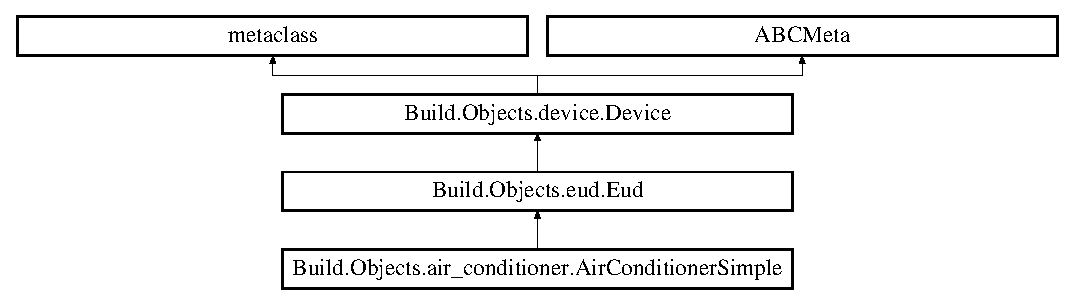
\includegraphics[height=3.648208cm]{class_build_1_1_objects_1_1air__conditioner_1_1_air_conditioner_simple}
\end{center}
\end{figure}
\subsection*{Public Member Functions}
\begin{DoxyCompactItemize}
\item 
def \hyperlink{class_build_1_1_objects_1_1air__conditioner_1_1_air_conditioner_simple_a851cc811958a860f2796cbb5af4f40da}{\+\_\+\+\_\+init\+\_\+\+\_\+} (self, device\+\_\+id, supervisor, msg\+\_\+latency=0, schedule=None, multiday=0, total\+\_\+runtime=S\+E\+C\+O\+N\+D\+S\+\_\+\+I\+N\+\_\+\+D\+AY, time=0, connected\+\_\+devices=None, compressor\+\_\+operating\+\_\+power=500.\+0, initial\+\_\+temp=25.\+0, temp\+\_\+max\+\_\+delta=0.\+5, initial\+\_\+set\+\_\+point=23.\+0, price\+\_\+to\+\_\+setpoint=None, temperature\+\_\+schedule=None, compressor\+\_\+cooling\+\_\+rate=2.\+0, heat\+\_\+exchange\+\_\+rate=0.\+1, modulation\+\_\+interval=300)
\item 
def \hyperlink{class_build_1_1_objects_1_1air__conditioner_1_1_air_conditioner_simple_a780672ba57c94495b1203d5da8715ec8}{schedule\+\_\+outdoor\+\_\+temperature\+\_\+events} (self, temperature\+\_\+schedule, total\+\_\+runtime)
\begin{DoxyCompactList}\small\item\em Schedules all of the temperature change events each day for the entire duration of the simulation. \end{DoxyCompactList}\item 
def \hyperlink{class_build_1_1_objects_1_1air__conditioner_1_1_air_conditioner_simple_ace754a3c9581817b5bbce2394da2163a}{reassess\+\_\+setpoint} (self)
\begin{DoxyCompactList}\small\item\em Given the current price of the device, determine what the current temperature setpoint should be. \end{DoxyCompactList}\item 
def \hyperlink{class_build_1_1_objects_1_1air__conditioner_1_1_air_conditioner_simple_ac637b8d11556eea36880d3947b5c00c0}{get\+\_\+setpoint\+\_\+from\+\_\+price} (self, price)
\begin{DoxyCompactList}\small\item\em Returns the setpoint value from the given price by finding the next largest price-\/setpoint value in the input setpoint dictionary. \end{DoxyCompactList}\item 
\mbox{\Hypertarget{class_build_1_1_objects_1_1air__conditioner_1_1_air_conditioner_simple_a641bfc9644a25a253f17c0e508ffa1ae}\label{class_build_1_1_objects_1_1air__conditioner_1_1_air_conditioner_simple_a641bfc9644a25a253f17c0e508ffa1ae}} 
def \hyperlink{class_build_1_1_objects_1_1air__conditioner_1_1_air_conditioner_simple_a641bfc9644a25a253f17c0e508ffa1ae}{adjust\+\_\+internal\+\_\+temperature} (self)
\begin{DoxyCompactList}\small\item\em Adjusts the internal temperature of the a/c based on the indoor/outdoor temperature difference. \end{DoxyCompactList}\item 
def \hyperlink{class_build_1_1_objects_1_1air__conditioner_1_1_air_conditioner_simple_a16c1867273e35cce644563ed0a33fcc9}{control\+\_\+compressor\+\_\+operation} (self)
\begin{DoxyCompactList}\small\item\em Given the current internal temperature of the air conditioner and the desired setpoint, determine whether the compressor should be on. \end{DoxyCompactList}\item 
def \hyperlink{class_build_1_1_objects_1_1air__conditioner_1_1_air_conditioner_simple_aa758ea8ab27c611b7e661f3eea7df4e6}{turn\+\_\+on\+\_\+compressor} (self)
\begin{DoxyCompactList}\small\item\em Turns on the compressor. \end{DoxyCompactList}\item 
def \hyperlink{class_build_1_1_objects_1_1air__conditioner_1_1_air_conditioner_simple_affced4fc3f6e8260d31c1690a8b5614d}{turn\+\_\+off\+\_\+compressor} (self)
\begin{DoxyCompactList}\small\item\em Turns off the compressor. \end{DoxyCompactList}\item 
def \hyperlink{class_build_1_1_objects_1_1air__conditioner_1_1_air_conditioner_simple_aafc4201ae9e6e9f297df07fc03f89be2}{update\+\_\+outdoor\+\_\+temperature} (self, new\+\_\+temperature)
\begin{DoxyCompactList}\small\item\em Refresh the current outdoor temperature value. \end{DoxyCompactList}\item 
def \hyperlink{class_build_1_1_objects_1_1air__conditioner_1_1_air_conditioner_simple_aa9fa855099f3b2d1db0726cc639c5026}{end\+\_\+internal\+\_\+operation} (self)
\begin{DoxyCompactList}\small\item\em Air conditioner will shut off compressor whenever device shuts off. \end{DoxyCompactList}\item 
\mbox{\Hypertarget{class_build_1_1_objects_1_1air__conditioner_1_1_air_conditioner_simple_a33d8fdca95127232bd3183d42d83c941}\label{class_build_1_1_objects_1_1air__conditioner_1_1_air_conditioner_simple_a33d8fdca95127232bd3183d42d83c941}} 
def \hyperlink{class_build_1_1_objects_1_1air__conditioner_1_1_air_conditioner_simple_a33d8fdca95127232bd3183d42d83c941}{begin\+\_\+internal\+\_\+operation} (self)
\begin{DoxyCompactList}\small\item\em Air conditioner does not have startup behavior. \end{DoxyCompactList}\item 
\mbox{\Hypertarget{class_build_1_1_objects_1_1air__conditioner_1_1_air_conditioner_simple_ae44edec63419de6b2bb9ea0bd93161e0}\label{class_build_1_1_objects_1_1air__conditioner_1_1_air_conditioner_simple_ae44edec63419de6b2bb9ea0bd93161e0}} 
def \hyperlink{class_build_1_1_objects_1_1air__conditioner_1_1_air_conditioner_simple_ae44edec63419de6b2bb9ea0bd93161e0}{update\+\_\+state} (self)
\begin{DoxyCompactList}\small\item\em Updates the state of the air conditioner by determining its internal temperature, desired setpoint, and hence desired. \end{DoxyCompactList}\item 
def \hyperlink{class_build_1_1_objects_1_1air__conditioner_1_1_air_conditioner_simple_ad127746965293e7973e69a00a701e54d}{calculate\+\_\+desired\+\_\+power\+\_\+level} (self)
\begin{DoxyCompactList}\small\item\em This air conditioner consumes what it requires to run the compressor if the compressor should be on. \end{DoxyCompactList}\item 
def \hyperlink{class_build_1_1_objects_1_1air__conditioner_1_1_air_conditioner_simple_af810a3fced1cc73099a33e4f4020a65e}{respond\+\_\+to\+\_\+power} (self, received\+\_\+power)
\begin{DoxyCompactList}\small\item\em When this Air Conditioner receives power, if it is sufficient for its needs it turns the compressor on. \end{DoxyCompactList}\item 
\mbox{\Hypertarget{class_build_1_1_objects_1_1air__conditioner_1_1_air_conditioner_simple_a13cb6a7cf5b10f62aaabd50ad902a756}\label{class_build_1_1_objects_1_1air__conditioner_1_1_air_conditioner_simple_a13cb6a7cf5b10f62aaabd50ad902a756}} 
def {\bfseries device\+\_\+specific\+\_\+calcs} (self)
\end{DoxyCompactItemize}
\subsection*{Additional Inherited Members}


\subsection{Constructor \& Destructor Documentation}
\mbox{\Hypertarget{class_build_1_1_objects_1_1air__conditioner_1_1_air_conditioner_simple_a851cc811958a860f2796cbb5af4f40da}\label{class_build_1_1_objects_1_1air__conditioner_1_1_air_conditioner_simple_a851cc811958a860f2796cbb5af4f40da}} 
\index{Build\+::\+Objects\+::air\+\_\+conditioner\+::\+Air\+Conditioner\+Simple@{Build\+::\+Objects\+::air\+\_\+conditioner\+::\+Air\+Conditioner\+Simple}!\+\_\+\+\_\+init\+\_\+\+\_\+@{\+\_\+\+\_\+init\+\_\+\+\_\+}}
\index{\+\_\+\+\_\+init\+\_\+\+\_\+@{\+\_\+\+\_\+init\+\_\+\+\_\+}!Build\+::\+Objects\+::air\+\_\+conditioner\+::\+Air\+Conditioner\+Simple@{Build\+::\+Objects\+::air\+\_\+conditioner\+::\+Air\+Conditioner\+Simple}}
\subsubsection{\texorpdfstring{\+\_\+\+\_\+init\+\_\+\+\_\+()}{\_\_init\_\_()}}
{\footnotesize\ttfamily def Build.\+Objects.\+air\+\_\+conditioner.\+Air\+Conditioner\+Simple.\+\_\+\+\_\+init\+\_\+\+\_\+ (\begin{DoxyParamCaption}\item[{}]{self,  }\item[{}]{device\+\_\+id,  }\item[{}]{supervisor,  }\item[{}]{msg\+\_\+latency = {\ttfamily 0},  }\item[{}]{schedule = {\ttfamily None},  }\item[{}]{multiday = {\ttfamily 0},  }\item[{}]{total\+\_\+runtime = {\ttfamily SECONDS\+\_\+IN\+\_\+DAY},  }\item[{}]{time = {\ttfamily 0},  }\item[{}]{connected\+\_\+devices = {\ttfamily None},  }\item[{}]{compressor\+\_\+operating\+\_\+power = {\ttfamily 500.0},  }\item[{}]{initial\+\_\+temp = {\ttfamily 25.0},  }\item[{}]{temp\+\_\+max\+\_\+delta = {\ttfamily 0.5},  }\item[{}]{initial\+\_\+set\+\_\+point = {\ttfamily 23.0},  }\item[{}]{price\+\_\+to\+\_\+setpoint = {\ttfamily None},  }\item[{}]{temperature\+\_\+schedule = {\ttfamily None},  }\item[{}]{compressor\+\_\+cooling\+\_\+rate = {\ttfamily 2.0},  }\item[{}]{heat\+\_\+exchange\+\_\+rate = {\ttfamily 0.1},  }\item[{}]{modulation\+\_\+interval = {\ttfamily 300} }\end{DoxyParamCaption})}


\begin{DoxyParams}{Parameters}
{\em compressor\+\_\+operating\+\_\+power} & how much energy the device requires to keep the compressor in operation \\
\hline
{\em compressor\+\_\+temp\+\_\+rate} & the cooling rate at the air conditioner (degrees C / hour). \\
\hline
{\em initial\+\_\+temp} & The initial internal temperature of the air conditioner \\
\hline
{\em initial\+\_\+setpoint} & initial setpoint of this device \\
\hline
{\em heat\+\_\+exchange\+\_\+rate} & the rate of change in temperature as a result of the difference between internal and external temperature \\
\hline
{\em price\+\_\+to\+\_\+setpoint} & a list of lists of price, setpoint for this device to modify setpoint based on price \\
\hline
\end{DoxyParams}


\subsection{Member Function Documentation}
\mbox{\Hypertarget{class_build_1_1_objects_1_1air__conditioner_1_1_air_conditioner_simple_ad127746965293e7973e69a00a701e54d}\label{class_build_1_1_objects_1_1air__conditioner_1_1_air_conditioner_simple_ad127746965293e7973e69a00a701e54d}} 
\index{Build\+::\+Objects\+::air\+\_\+conditioner\+::\+Air\+Conditioner\+Simple@{Build\+::\+Objects\+::air\+\_\+conditioner\+::\+Air\+Conditioner\+Simple}!calculate\+\_\+desired\+\_\+power\+\_\+level@{calculate\+\_\+desired\+\_\+power\+\_\+level}}
\index{calculate\+\_\+desired\+\_\+power\+\_\+level@{calculate\+\_\+desired\+\_\+power\+\_\+level}!Build\+::\+Objects\+::air\+\_\+conditioner\+::\+Air\+Conditioner\+Simple@{Build\+::\+Objects\+::air\+\_\+conditioner\+::\+Air\+Conditioner\+Simple}}
\subsubsection{\texorpdfstring{calculate\+\_\+desired\+\_\+power\+\_\+level()}{calculate\_desired\_power\_level()}}
{\footnotesize\ttfamily def Build.\+Objects.\+air\+\_\+conditioner.\+Air\+Conditioner\+Simple.\+calculate\+\_\+desired\+\_\+power\+\_\+level (\begin{DoxyParamCaption}\item[{}]{self }\end{DoxyParamCaption})}



This air conditioner consumes what it requires to run the compressor if the compressor should be on. 

\begin{DoxyReturn}{Returns}
the amount of power this a/c would like to consume 
\end{DoxyReturn}
\mbox{\Hypertarget{class_build_1_1_objects_1_1air__conditioner_1_1_air_conditioner_simple_a16c1867273e35cce644563ed0a33fcc9}\label{class_build_1_1_objects_1_1air__conditioner_1_1_air_conditioner_simple_a16c1867273e35cce644563ed0a33fcc9}} 
\index{Build\+::\+Objects\+::air\+\_\+conditioner\+::\+Air\+Conditioner\+Simple@{Build\+::\+Objects\+::air\+\_\+conditioner\+::\+Air\+Conditioner\+Simple}!control\+\_\+compressor\+\_\+operation@{control\+\_\+compressor\+\_\+operation}}
\index{control\+\_\+compressor\+\_\+operation@{control\+\_\+compressor\+\_\+operation}!Build\+::\+Objects\+::air\+\_\+conditioner\+::\+Air\+Conditioner\+Simple@{Build\+::\+Objects\+::air\+\_\+conditioner\+::\+Air\+Conditioner\+Simple}}
\subsubsection{\texorpdfstring{control\+\_\+compressor\+\_\+operation()}{control\_compressor\_operation()}}
{\footnotesize\ttfamily def Build.\+Objects.\+air\+\_\+conditioner.\+Air\+Conditioner\+Simple.\+control\+\_\+compressor\+\_\+operation (\begin{DoxyParamCaption}\item[{}]{self }\end{DoxyParamCaption})}



Given the current internal temperature of the air conditioner and the desired setpoint, determine whether the compressor should be on. 

If the compressor should not be on, turn it off. If it should be, record that so we can request the necessary power in order to turn it on. \mbox{\Hypertarget{class_build_1_1_objects_1_1air__conditioner_1_1_air_conditioner_simple_aa9fa855099f3b2d1db0726cc639c5026}\label{class_build_1_1_objects_1_1air__conditioner_1_1_air_conditioner_simple_aa9fa855099f3b2d1db0726cc639c5026}} 
\index{Build\+::\+Objects\+::air\+\_\+conditioner\+::\+Air\+Conditioner\+Simple@{Build\+::\+Objects\+::air\+\_\+conditioner\+::\+Air\+Conditioner\+Simple}!end\+\_\+internal\+\_\+operation@{end\+\_\+internal\+\_\+operation}}
\index{end\+\_\+internal\+\_\+operation@{end\+\_\+internal\+\_\+operation}!Build\+::\+Objects\+::air\+\_\+conditioner\+::\+Air\+Conditioner\+Simple@{Build\+::\+Objects\+::air\+\_\+conditioner\+::\+Air\+Conditioner\+Simple}}
\subsubsection{\texorpdfstring{end\+\_\+internal\+\_\+operation()}{end\_internal\_operation()}}
{\footnotesize\ttfamily def Build.\+Objects.\+air\+\_\+conditioner.\+Air\+Conditioner\+Simple.\+end\+\_\+internal\+\_\+operation (\begin{DoxyParamCaption}\item[{}]{self }\end{DoxyParamCaption})}



Air conditioner will shut off compressor whenever device shuts off. 

\mbox{\Hypertarget{class_build_1_1_objects_1_1air__conditioner_1_1_air_conditioner_simple_ac637b8d11556eea36880d3947b5c00c0}\label{class_build_1_1_objects_1_1air__conditioner_1_1_air_conditioner_simple_ac637b8d11556eea36880d3947b5c00c0}} 
\index{Build\+::\+Objects\+::air\+\_\+conditioner\+::\+Air\+Conditioner\+Simple@{Build\+::\+Objects\+::air\+\_\+conditioner\+::\+Air\+Conditioner\+Simple}!get\+\_\+setpoint\+\_\+from\+\_\+price@{get\+\_\+setpoint\+\_\+from\+\_\+price}}
\index{get\+\_\+setpoint\+\_\+from\+\_\+price@{get\+\_\+setpoint\+\_\+from\+\_\+price}!Build\+::\+Objects\+::air\+\_\+conditioner\+::\+Air\+Conditioner\+Simple@{Build\+::\+Objects\+::air\+\_\+conditioner\+::\+Air\+Conditioner\+Simple}}
\subsubsection{\texorpdfstring{get\+\_\+setpoint\+\_\+from\+\_\+price()}{get\_setpoint\_from\_price()}}
{\footnotesize\ttfamily def Build.\+Objects.\+air\+\_\+conditioner.\+Air\+Conditioner\+Simple.\+get\+\_\+setpoint\+\_\+from\+\_\+price (\begin{DoxyParamCaption}\item[{}]{self,  }\item[{}]{price }\end{DoxyParamCaption})}



Returns the setpoint value from the given price by finding the next largest price-\/setpoint value in the input setpoint dictionary. 

\mbox{\Hypertarget{class_build_1_1_objects_1_1air__conditioner_1_1_air_conditioner_simple_ace754a3c9581817b5bbce2394da2163a}\label{class_build_1_1_objects_1_1air__conditioner_1_1_air_conditioner_simple_ace754a3c9581817b5bbce2394da2163a}} 
\index{Build\+::\+Objects\+::air\+\_\+conditioner\+::\+Air\+Conditioner\+Simple@{Build\+::\+Objects\+::air\+\_\+conditioner\+::\+Air\+Conditioner\+Simple}!reassess\+\_\+setpoint@{reassess\+\_\+setpoint}}
\index{reassess\+\_\+setpoint@{reassess\+\_\+setpoint}!Build\+::\+Objects\+::air\+\_\+conditioner\+::\+Air\+Conditioner\+Simple@{Build\+::\+Objects\+::air\+\_\+conditioner\+::\+Air\+Conditioner\+Simple}}
\subsubsection{\texorpdfstring{reassess\+\_\+setpoint()}{reassess\_setpoint()}}
{\footnotesize\ttfamily def Build.\+Objects.\+air\+\_\+conditioner.\+Air\+Conditioner\+Simple.\+reassess\+\_\+setpoint (\begin{DoxyParamCaption}\item[{}]{self }\end{DoxyParamCaption})}



Given the current price of the device, determine what the current temperature setpoint should be. 

\mbox{\Hypertarget{class_build_1_1_objects_1_1air__conditioner_1_1_air_conditioner_simple_af810a3fced1cc73099a33e4f4020a65e}\label{class_build_1_1_objects_1_1air__conditioner_1_1_air_conditioner_simple_af810a3fced1cc73099a33e4f4020a65e}} 
\index{Build\+::\+Objects\+::air\+\_\+conditioner\+::\+Air\+Conditioner\+Simple@{Build\+::\+Objects\+::air\+\_\+conditioner\+::\+Air\+Conditioner\+Simple}!respond\+\_\+to\+\_\+power@{respond\+\_\+to\+\_\+power}}
\index{respond\+\_\+to\+\_\+power@{respond\+\_\+to\+\_\+power}!Build\+::\+Objects\+::air\+\_\+conditioner\+::\+Air\+Conditioner\+Simple@{Build\+::\+Objects\+::air\+\_\+conditioner\+::\+Air\+Conditioner\+Simple}}
\subsubsection{\texorpdfstring{respond\+\_\+to\+\_\+power()}{respond\_to\_power()}}
{\footnotesize\ttfamily def Build.\+Objects.\+air\+\_\+conditioner.\+Air\+Conditioner\+Simple.\+respond\+\_\+to\+\_\+power (\begin{DoxyParamCaption}\item[{}]{self,  }\item[{}]{received\+\_\+power }\end{DoxyParamCaption})}



When this Air Conditioner receives power, if it is sufficient for its needs it turns the compressor on. 

Otherwise, if the compressor can no longer operate turn it off. \mbox{\Hypertarget{class_build_1_1_objects_1_1air__conditioner_1_1_air_conditioner_simple_a780672ba57c94495b1203d5da8715ec8}\label{class_build_1_1_objects_1_1air__conditioner_1_1_air_conditioner_simple_a780672ba57c94495b1203d5da8715ec8}} 
\index{Build\+::\+Objects\+::air\+\_\+conditioner\+::\+Air\+Conditioner\+Simple@{Build\+::\+Objects\+::air\+\_\+conditioner\+::\+Air\+Conditioner\+Simple}!schedule\+\_\+outdoor\+\_\+temperature\+\_\+events@{schedule\+\_\+outdoor\+\_\+temperature\+\_\+events}}
\index{schedule\+\_\+outdoor\+\_\+temperature\+\_\+events@{schedule\+\_\+outdoor\+\_\+temperature\+\_\+events}!Build\+::\+Objects\+::air\+\_\+conditioner\+::\+Air\+Conditioner\+Simple@{Build\+::\+Objects\+::air\+\_\+conditioner\+::\+Air\+Conditioner\+Simple}}
\subsubsection{\texorpdfstring{schedule\+\_\+outdoor\+\_\+temperature\+\_\+events()}{schedule\_outdoor\_temperature\_events()}}
{\footnotesize\ttfamily def Build.\+Objects.\+air\+\_\+conditioner.\+Air\+Conditioner\+Simple.\+schedule\+\_\+outdoor\+\_\+temperature\+\_\+events (\begin{DoxyParamCaption}\item[{}]{self,  }\item[{}]{temperature\+\_\+schedule,  }\item[{}]{total\+\_\+runtime }\end{DoxyParamCaption})}



Schedules all of the temperature change events each day for the entire duration of the simulation. 


\begin{DoxyParams}{Parameters}
{\em temperature\+\_\+schedule} & a list of tuples of (time, temperature) for outdoor temperatures. \\
\hline
\end{DoxyParams}
\mbox{\Hypertarget{class_build_1_1_objects_1_1air__conditioner_1_1_air_conditioner_simple_affced4fc3f6e8260d31c1690a8b5614d}\label{class_build_1_1_objects_1_1air__conditioner_1_1_air_conditioner_simple_affced4fc3f6e8260d31c1690a8b5614d}} 
\index{Build\+::\+Objects\+::air\+\_\+conditioner\+::\+Air\+Conditioner\+Simple@{Build\+::\+Objects\+::air\+\_\+conditioner\+::\+Air\+Conditioner\+Simple}!turn\+\_\+off\+\_\+compressor@{turn\+\_\+off\+\_\+compressor}}
\index{turn\+\_\+off\+\_\+compressor@{turn\+\_\+off\+\_\+compressor}!Build\+::\+Objects\+::air\+\_\+conditioner\+::\+Air\+Conditioner\+Simple@{Build\+::\+Objects\+::air\+\_\+conditioner\+::\+Air\+Conditioner\+Simple}}
\subsubsection{\texorpdfstring{turn\+\_\+off\+\_\+compressor()}{turn\_off\_compressor()}}
{\footnotesize\ttfamily def Build.\+Objects.\+air\+\_\+conditioner.\+Air\+Conditioner\+Simple.\+turn\+\_\+off\+\_\+compressor (\begin{DoxyParamCaption}\item[{}]{self }\end{DoxyParamCaption})}



Turns off the compressor. 

\mbox{\Hypertarget{class_build_1_1_objects_1_1air__conditioner_1_1_air_conditioner_simple_aa758ea8ab27c611b7e661f3eea7df4e6}\label{class_build_1_1_objects_1_1air__conditioner_1_1_air_conditioner_simple_aa758ea8ab27c611b7e661f3eea7df4e6}} 
\index{Build\+::\+Objects\+::air\+\_\+conditioner\+::\+Air\+Conditioner\+Simple@{Build\+::\+Objects\+::air\+\_\+conditioner\+::\+Air\+Conditioner\+Simple}!turn\+\_\+on\+\_\+compressor@{turn\+\_\+on\+\_\+compressor}}
\index{turn\+\_\+on\+\_\+compressor@{turn\+\_\+on\+\_\+compressor}!Build\+::\+Objects\+::air\+\_\+conditioner\+::\+Air\+Conditioner\+Simple@{Build\+::\+Objects\+::air\+\_\+conditioner\+::\+Air\+Conditioner\+Simple}}
\subsubsection{\texorpdfstring{turn\+\_\+on\+\_\+compressor()}{turn\_on\_compressor()}}
{\footnotesize\ttfamily def Build.\+Objects.\+air\+\_\+conditioner.\+Air\+Conditioner\+Simple.\+turn\+\_\+on\+\_\+compressor (\begin{DoxyParamCaption}\item[{}]{self }\end{DoxyParamCaption})}



Turns on the compressor. 

\mbox{\Hypertarget{class_build_1_1_objects_1_1air__conditioner_1_1_air_conditioner_simple_aafc4201ae9e6e9f297df07fc03f89be2}\label{class_build_1_1_objects_1_1air__conditioner_1_1_air_conditioner_simple_aafc4201ae9e6e9f297df07fc03f89be2}} 
\index{Build\+::\+Objects\+::air\+\_\+conditioner\+::\+Air\+Conditioner\+Simple@{Build\+::\+Objects\+::air\+\_\+conditioner\+::\+Air\+Conditioner\+Simple}!update\+\_\+outdoor\+\_\+temperature@{update\+\_\+outdoor\+\_\+temperature}}
\index{update\+\_\+outdoor\+\_\+temperature@{update\+\_\+outdoor\+\_\+temperature}!Build\+::\+Objects\+::air\+\_\+conditioner\+::\+Air\+Conditioner\+Simple@{Build\+::\+Objects\+::air\+\_\+conditioner\+::\+Air\+Conditioner\+Simple}}
\subsubsection{\texorpdfstring{update\+\_\+outdoor\+\_\+temperature()}{update\_outdoor\_temperature()}}
{\footnotesize\ttfamily def Build.\+Objects.\+air\+\_\+conditioner.\+Air\+Conditioner\+Simple.\+update\+\_\+outdoor\+\_\+temperature (\begin{DoxyParamCaption}\item[{}]{self,  }\item[{}]{new\+\_\+temperature }\end{DoxyParamCaption})}



Refresh the current outdoor temperature value. 


\begin{DoxyParams}{Parameters}
{\em new\+\_\+temperature} & the new outdoor temperature value \\
\hline
\end{DoxyParams}


The documentation for this class was generated from the following file\+:\begin{DoxyCompactItemize}
\item 
Build/\+Objects/air\+\_\+conditioner.\+py\end{DoxyCompactItemize}

\hypertarget{class_build_1_1_objects_1_1battery_1_1_battery}{}\section{Build.\+Objects.\+battery.\+Battery Class Reference}
\label{class_build_1_1_objects_1_1battery_1_1_battery}\index{Build.\+Objects.\+battery.\+Battery@{Build.\+Objects.\+battery.\+Battery}}
Inheritance diagram for Build.\+Objects.\+battery.\+Battery\+:\begin{figure}[H]
\begin{center}
\leavevmode
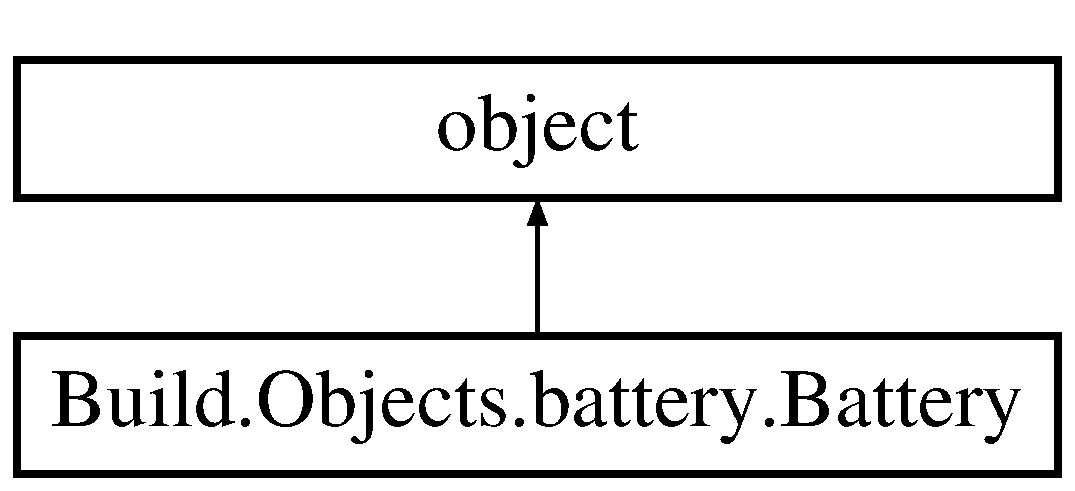
\includegraphics[height=2.000000cm]{class_build_1_1_objects_1_1battery_1_1_battery}
\end{center}
\end{figure}
\subsection*{Classes}
\begin{DoxyCompactItemize}
\item 
class \hyperlink{class_build_1_1_objects_1_1battery_1_1_battery_1_1_battery_charging_preference}{Battery\+Charging\+Preference}
\begin{DoxyCompactList}\small\item\em \hyperlink{class_build_1_1_objects_1_1battery_1_1_battery}{Battery} charging preference is based on the batteries current state of charge (soc). \end{DoxyCompactList}\end{DoxyCompactItemize}
\subsection*{Public Member Functions}
\begin{DoxyCompactItemize}
\item 
def \hyperlink{class_build_1_1_objects_1_1battery_1_1_battery_a4f033824699b9a467a337561a41f024a}{\+\_\+\+\_\+init\+\_\+\+\_\+} (self, battery\+\_\+id, price\+\_\+logic, capacity, max\+\_\+charge\+\_\+rate, max\+\_\+discharge\+\_\+rate, preferred\+\_\+charge\+\_\+rate=None, preferred\+\_\+discharge\+\_\+rate=None, starting\+\_\+soc=1.\+0, update\+\_\+frequency=300)
\begin{DoxyCompactList}\small\item\em Initializes the battery to be contained within a grid controller. \end{DoxyCompactList}\item 
\mbox{\Hypertarget{class_build_1_1_objects_1_1battery_1_1_battery_ac493263e624c98ce6688973e35cd745b}\label{class_build_1_1_objects_1_1battery_1_1_battery_ac493263e624c98ce6688973e35cd745b}} 
def \hyperlink{class_build_1_1_objects_1_1battery_1_1_battery_ac493263e624c98ce6688973e35cd745b}{get\+\_\+load} (self)
\begin{DoxyCompactList}\small\item\em Returns the current load on the battery. \end{DoxyCompactList}\item 
\mbox{\Hypertarget{class_build_1_1_objects_1_1battery_1_1_battery_a111980cd30f418ba49e64ca9b89313d4}\label{class_build_1_1_objects_1_1battery_1_1_battery_a111980cd30f418ba49e64ca9b89313d4}} 
def \hyperlink{class_build_1_1_objects_1_1battery_1_1_battery_a111980cd30f418ba49e64ca9b89313d4}{get\+\_\+current\+\_\+soc} (self)
\begin{DoxyCompactList}\small\item\em Returns the batteries current state of charge. \end{DoxyCompactList}\item 
\mbox{\Hypertarget{class_build_1_1_objects_1_1battery_1_1_battery_a7f98f0d9fb7608837c17618b799c7e55}\label{class_build_1_1_objects_1_1battery_1_1_battery_a7f98f0d9fb7608837c17618b799c7e55}} 
def \hyperlink{class_build_1_1_objects_1_1battery_1_1_battery_a7f98f0d9fb7608837c17618b799c7e55}{get\+\_\+charging\+\_\+preference} (self)
\begin{DoxyCompactList}\small\item\em Returns the value of the current batteries charging preference (1 if discharge, 0 if neutral, -\/1 if discharge) \end{DoxyCompactList}\item 
\mbox{\Hypertarget{class_build_1_1_objects_1_1battery_1_1_battery_ace39c87e0ab087c9f7d07c8a5f645fc4}\label{class_build_1_1_objects_1_1battery_1_1_battery_ace39c87e0ab087c9f7d07c8a5f645fc4}} 
def \hyperlink{class_build_1_1_objects_1_1battery_1_1_battery_ace39c87e0ab087c9f7d07c8a5f645fc4}{get\+\_\+max\+\_\+charge\+\_\+rate} (self)
\begin{DoxyCompactList}\small\item\em Getter for max charge rate. \end{DoxyCompactList}\item 
\mbox{\Hypertarget{class_build_1_1_objects_1_1battery_1_1_battery_a506889af4ebe7834352be77633a4a6f0}\label{class_build_1_1_objects_1_1battery_1_1_battery_a506889af4ebe7834352be77633a4a6f0}} 
def \hyperlink{class_build_1_1_objects_1_1battery_1_1_battery_a506889af4ebe7834352be77633a4a6f0}{get\+\_\+max\+\_\+discharge\+\_\+rate} (self)
\begin{DoxyCompactList}\small\item\em Getter for max discharge rate. \end{DoxyCompactList}\item 
\mbox{\Hypertarget{class_build_1_1_objects_1_1battery_1_1_battery_a36c84b4ac8194d64a0a319b626514e0f}\label{class_build_1_1_objects_1_1battery_1_1_battery_a36c84b4ac8194d64a0a319b626514e0f}} 
def {\bfseries get\+\_\+update\+\_\+frequency} (self)
\item 
def \hyperlink{class_build_1_1_objects_1_1battery_1_1_battery_a8f464a9edbd9a2efbe609477d004ccb1}{get\+\_\+optimal\+\_\+charge\+\_\+rate} (self)
\begin{DoxyCompactList}\small\item\em Based on the current state of charge determine what the optimal charge rate for the battery is. \end{DoxyCompactList}\item 
def \hyperlink{class_build_1_1_objects_1_1battery_1_1_battery_a246c9aa9c3d54e71519b0a20a8ea350b}{add\+\_\+load} (self, extra\+\_\+load)
\begin{DoxyCompactList}\small\item\em Tries to add a new load to the battery, never exceeding the battery\textquotesingle{}s maximum discharge or charge rate. \end{DoxyCompactList}\item 
\mbox{\Hypertarget{class_build_1_1_objects_1_1battery_1_1_battery_a1820a5bff8f3d5d46f8d32ff73e1006c}\label{class_build_1_1_objects_1_1battery_1_1_battery_a1820a5bff8f3d5d46f8d32ff73e1006c}} 
def \hyperlink{class_build_1_1_objects_1_1battery_1_1_battery_a1820a5bff8f3d5d46f8d32ff73e1006c}{clear\+\_\+load} (self)
\begin{DoxyCompactList}\small\item\em Resets the battery load to zero. \end{DoxyCompactList}\item 
def \hyperlink{class_build_1_1_objects_1_1battery_1_1_battery_a246d8921279b7cb78a0f6b33f2309085}{update\+\_\+state} (self, time, price, average\+\_\+price, price\+\_\+history)
\begin{DoxyCompactList}\small\item\em Updates the state of charge and power levels of the battery reflecting current time. \end{DoxyCompactList}\item 
def \hyperlink{class_build_1_1_objects_1_1battery_1_1_battery_a2c343f81c849a4b8d6de5de9f19ebc98}{recalc\+\_\+charge\+\_\+preference} (self)
\item 
def \hyperlink{class_build_1_1_objects_1_1battery_1_1_battery_aa4838ab445d5c20f9c27752ffc911c6e}{build\+\_\+battery\+\_\+log\+\_\+notation} (self, message=\char`\"{}\char`\"{}, value=None)
\begin{DoxyCompactList}\small\item\em Builds a logging message for this battery, always including information about its state of charge and battery preference. \end{DoxyCompactList}\end{DoxyCompactItemize}
\subsection*{Public Attributes}
\begin{DoxyCompactItemize}
\item 
\mbox{\Hypertarget{class_build_1_1_objects_1_1battery_1_1_battery_afa91328477ff0492e6676ad1f0f02cb3}\label{class_build_1_1_objects_1_1battery_1_1_battery_afa91328477ff0492e6676ad1f0f02cb3}} 
{\bfseries sum\+\_\+charge\+\_\+wh}
\item 
\mbox{\Hypertarget{class_build_1_1_objects_1_1battery_1_1_battery_a29e1aeb292abeb444b5fb2ca05749c96}\label{class_build_1_1_objects_1_1battery_1_1_battery_a29e1aeb292abeb444b5fb2ca05749c96}} 
{\bfseries sum\+\_\+discharge\+\_\+wh}
\end{DoxyCompactItemize}


\subsection{Constructor \& Destructor Documentation}
\mbox{\Hypertarget{class_build_1_1_objects_1_1battery_1_1_battery_a4f033824699b9a467a337561a41f024a}\label{class_build_1_1_objects_1_1battery_1_1_battery_a4f033824699b9a467a337561a41f024a}} 
\index{Build\+::\+Objects\+::battery\+::\+Battery@{Build\+::\+Objects\+::battery\+::\+Battery}!\+\_\+\+\_\+init\+\_\+\+\_\+@{\+\_\+\+\_\+init\+\_\+\+\_\+}}
\index{\+\_\+\+\_\+init\+\_\+\+\_\+@{\+\_\+\+\_\+init\+\_\+\+\_\+}!Build\+::\+Objects\+::battery\+::\+Battery@{Build\+::\+Objects\+::battery\+::\+Battery}}
\subsubsection{\texorpdfstring{\+\_\+\+\_\+init\+\_\+\+\_\+()}{\_\_init\_\_()}}
{\footnotesize\ttfamily def Build.\+Objects.\+battery.\+Battery.\+\_\+\+\_\+init\+\_\+\+\_\+ (\begin{DoxyParamCaption}\item[{}]{self,  }\item[{}]{battery\+\_\+id,  }\item[{}]{price\+\_\+logic,  }\item[{}]{capacity,  }\item[{}]{max\+\_\+charge\+\_\+rate,  }\item[{}]{max\+\_\+discharge\+\_\+rate,  }\item[{}]{preferred\+\_\+charge\+\_\+rate = {\ttfamily None},  }\item[{}]{preferred\+\_\+discharge\+\_\+rate = {\ttfamily None},  }\item[{}]{starting\+\_\+soc = {\ttfamily 1.0},  }\item[{}]{update\+\_\+frequency = {\ttfamily 300} }\end{DoxyParamCaption})}



Initializes the battery to be contained within a grid controller. 


\begin{DoxyParams}{Parameters}
{\em capacity} & the maximum charge capacity of the battery. Must be a double. \\
\hline
{\em preferred} & charge rate the preferred rate of charge for this battery. Defaults to max charge rate \\
\hline
{\em preferred} & discharge rate the preferred discharge rate for this battery. Defaults to max discharge rate \\
\hline
{\em starting\+\_\+soc} & the state of charge on initialization. Default 50\% \\
\hline
{\em update\+\_\+frequency} & how frequently to update the state of this battery. Defaults to every 5 minutes (300s) \\
\hline
\end{DoxyParams}


\subsection{Member Function Documentation}
\mbox{\Hypertarget{class_build_1_1_objects_1_1battery_1_1_battery_a246c9aa9c3d54e71519b0a20a8ea350b}\label{class_build_1_1_objects_1_1battery_1_1_battery_a246c9aa9c3d54e71519b0a20a8ea350b}} 
\index{Build\+::\+Objects\+::battery\+::\+Battery@{Build\+::\+Objects\+::battery\+::\+Battery}!add\+\_\+load@{add\+\_\+load}}
\index{add\+\_\+load@{add\+\_\+load}!Build\+::\+Objects\+::battery\+::\+Battery@{Build\+::\+Objects\+::battery\+::\+Battery}}
\subsubsection{\texorpdfstring{add\+\_\+load()}{add\_load()}}
{\footnotesize\ttfamily def Build.\+Objects.\+battery.\+Battery.\+add\+\_\+load (\begin{DoxyParamCaption}\item[{}]{self,  }\item[{}]{extra\+\_\+load }\end{DoxyParamCaption})}



Tries to add a new load to the battery, never exceeding the battery\textquotesingle{}s maximum discharge or charge rate. 

Call update state first to ensure valid state of charge and to update charging calculations before modification. 
\begin{DoxyParams}{Parameters}
{\em extra\+\_\+load} & the load to add from battery\textquotesingle{}s perspective (positive charge, negative discharge) \\
\hline
{\em return} & whatever value was added to the battery\textquotesingle{}s load (may not be full val. \\
\hline
\end{DoxyParams}
\mbox{\Hypertarget{class_build_1_1_objects_1_1battery_1_1_battery_aa4838ab445d5c20f9c27752ffc911c6e}\label{class_build_1_1_objects_1_1battery_1_1_battery_aa4838ab445d5c20f9c27752ffc911c6e}} 
\index{Build\+::\+Objects\+::battery\+::\+Battery@{Build\+::\+Objects\+::battery\+::\+Battery}!build\+\_\+battery\+\_\+log\+\_\+notation@{build\+\_\+battery\+\_\+log\+\_\+notation}}
\index{build\+\_\+battery\+\_\+log\+\_\+notation@{build\+\_\+battery\+\_\+log\+\_\+notation}!Build\+::\+Objects\+::battery\+::\+Battery@{Build\+::\+Objects\+::battery\+::\+Battery}}
\subsubsection{\texorpdfstring{build\+\_\+battery\+\_\+log\+\_\+notation()}{build\_battery\_log\_notation()}}
{\footnotesize\ttfamily def Build.\+Objects.\+battery.\+Battery.\+build\+\_\+battery\+\_\+log\+\_\+notation (\begin{DoxyParamCaption}\item[{}]{self,  }\item[{}]{message = {\ttfamily \char`\"{}\char`\"{}},  }\item[{}]{value = {\ttfamily None} }\end{DoxyParamCaption})}



Builds a logging message for this battery, always including information about its state of charge and battery preference. 


\begin{DoxyParams}{Parameters}
{\em message} & the message to add to logger \\
\hline
{\em value} & the value add to the logger \\
\hline
\end{DoxyParams}
\begin{DoxyReturn}{Returns}
a formatted string to include in the logger 
\end{DoxyReturn}
\mbox{\Hypertarget{class_build_1_1_objects_1_1battery_1_1_battery_a8f464a9edbd9a2efbe609477d004ccb1}\label{class_build_1_1_objects_1_1battery_1_1_battery_a8f464a9edbd9a2efbe609477d004ccb1}} 
\index{Build\+::\+Objects\+::battery\+::\+Battery@{Build\+::\+Objects\+::battery\+::\+Battery}!get\+\_\+optimal\+\_\+charge\+\_\+rate@{get\+\_\+optimal\+\_\+charge\+\_\+rate}}
\index{get\+\_\+optimal\+\_\+charge\+\_\+rate@{get\+\_\+optimal\+\_\+charge\+\_\+rate}!Build\+::\+Objects\+::battery\+::\+Battery@{Build\+::\+Objects\+::battery\+::\+Battery}}
\subsubsection{\texorpdfstring{get\+\_\+optimal\+\_\+charge\+\_\+rate()}{get\_optimal\_charge\_rate()}}
{\footnotesize\ttfamily def Build.\+Objects.\+battery.\+Battery.\+get\+\_\+optimal\+\_\+charge\+\_\+rate (\begin{DoxyParamCaption}\item[{}]{self }\end{DoxyParamCaption})}



Based on the current state of charge determine what the optimal charge rate for the battery is. 

\mbox{\Hypertarget{class_build_1_1_objects_1_1battery_1_1_battery_a2c343f81c849a4b8d6de5de9f19ebc98}\label{class_build_1_1_objects_1_1battery_1_1_battery_a2c343f81c849a4b8d6de5de9f19ebc98}} 
\index{Build\+::\+Objects\+::battery\+::\+Battery@{Build\+::\+Objects\+::battery\+::\+Battery}!recalc\+\_\+charge\+\_\+preference@{recalc\+\_\+charge\+\_\+preference}}
\index{recalc\+\_\+charge\+\_\+preference@{recalc\+\_\+charge\+\_\+preference}!Build\+::\+Objects\+::battery\+::\+Battery@{Build\+::\+Objects\+::battery\+::\+Battery}}
\subsubsection{\texorpdfstring{recalc\+\_\+charge\+\_\+preference()}{recalc\_charge\_preference()}}
{\footnotesize\ttfamily def Build.\+Objects.\+battery.\+Battery.\+recalc\+\_\+charge\+\_\+preference (\begin{DoxyParamCaption}\item[{}]{self }\end{DoxyParamCaption})}


\begin{DoxyParams}{Parameters}
{\em price\+\_\+stat} & the representative statistic to use to calculate it? \\
\hline
\end{DoxyParams}
\mbox{\Hypertarget{class_build_1_1_objects_1_1battery_1_1_battery_a246d8921279b7cb78a0f6b33f2309085}\label{class_build_1_1_objects_1_1battery_1_1_battery_a246d8921279b7cb78a0f6b33f2309085}} 
\index{Build\+::\+Objects\+::battery\+::\+Battery@{Build\+::\+Objects\+::battery\+::\+Battery}!update\+\_\+state@{update\+\_\+state}}
\index{update\+\_\+state@{update\+\_\+state}!Build\+::\+Objects\+::battery\+::\+Battery@{Build\+::\+Objects\+::battery\+::\+Battery}}
\subsubsection{\texorpdfstring{update\+\_\+state()}{update\_state()}}
{\footnotesize\ttfamily def Build.\+Objects.\+battery.\+Battery.\+update\+\_\+state (\begin{DoxyParamCaption}\item[{}]{self,  }\item[{}]{time,  }\item[{}]{price,  }\item[{}]{average\+\_\+price,  }\item[{}]{price\+\_\+history }\end{DoxyParamCaption})}



Updates the state of charge and power levels of the battery reflecting current time. 


\begin{DoxyParams}{Parameters}
{\em the} & time to update the battery\textquotesingle{}s local time to \\
\hline
{\em price} & the local price of the associated grid controller \\
\hline
{\em average} & price information on the average price of the grid controller \\
\hline
{\em hourly} & prices information on the hourly prices of the grid controller \\
\hline
\end{DoxyParams}


The documentation for this class was generated from the following file\+:\begin{DoxyCompactItemize}
\item 
Build/\+Objects/battery.\+py\end{DoxyCompactItemize}

\hypertarget{class_build_1_1_objects_1_1battery_1_1_battery_1_1_battery_charging_preference}{}\section{Build.\+Objects.\+battery.\+Battery.\+Battery\+Charging\+Preference Class Reference}
\label{class_build_1_1_objects_1_1battery_1_1_battery_1_1_battery_charging_preference}\index{Build.\+Objects.\+battery.\+Battery.\+Battery\+Charging\+Preference@{Build.\+Objects.\+battery.\+Battery.\+Battery\+Charging\+Preference}}


\hyperlink{class_build_1_1_objects_1_1battery_1_1_battery}{Battery} charging preference is based on the batteries current state of charge (soc).  


Inheritance diagram for Build.\+Objects.\+battery.\+Battery.\+Battery\+Charging\+Preference\+:\begin{figure}[H]
\begin{center}
\leavevmode
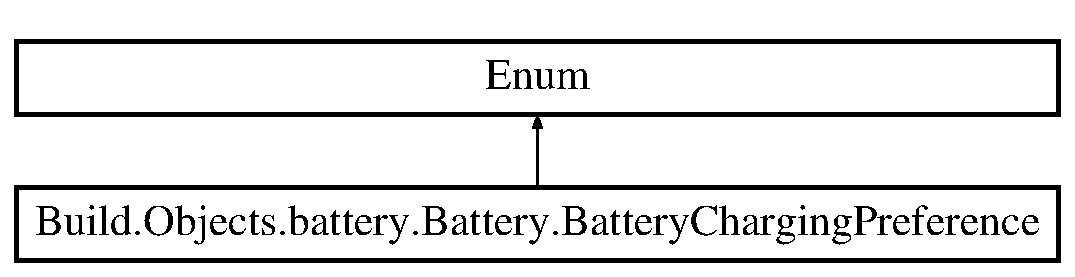
\includegraphics[height=2.000000cm]{class_build_1_1_objects_1_1battery_1_1_battery_1_1_battery_charging_preference}
\end{center}
\end{figure}
\subsection*{Static Public Attributes}
\begin{DoxyCompactItemize}
\item 
\mbox{\Hypertarget{class_build_1_1_objects_1_1battery_1_1_battery_1_1_battery_charging_preference_aaa23babf2d6aff6adbcc3b7baf0d2440}\label{class_build_1_1_objects_1_1battery_1_1_battery_1_1_battery_charging_preference_aaa23babf2d6aff6adbcc3b7baf0d2440}} 
int {\bfseries D\+I\+S\+C\+H\+A\+R\+GE} = -\/1
\item 
\mbox{\Hypertarget{class_build_1_1_objects_1_1battery_1_1_battery_1_1_battery_charging_preference_a5f96446b511011dbdf8ecb18b90326d6}\label{class_build_1_1_objects_1_1battery_1_1_battery_1_1_battery_charging_preference_a5f96446b511011dbdf8ecb18b90326d6}} 
int {\bfseries N\+E\+U\+T\+R\+AL} = 0
\item 
\mbox{\Hypertarget{class_build_1_1_objects_1_1battery_1_1_battery_1_1_battery_charging_preference_a7b7f064478fffacefa906b9955426ecd}\label{class_build_1_1_objects_1_1battery_1_1_battery_1_1_battery_charging_preference_a7b7f064478fffacefa906b9955426ecd}} 
int {\bfseries C\+H\+A\+R\+GE} = 1
\end{DoxyCompactItemize}


\subsection{Detailed Description}
\hyperlink{class_build_1_1_objects_1_1battery_1_1_battery}{Battery} charging preference is based on the batteries current state of charge (soc). 

Discharge indicates it would like to provide power, neutral no preference, charge to receive power. 

The documentation for this class was generated from the following file\+:\begin{DoxyCompactItemize}
\item 
Build/\+Objects/battery.\+py\end{DoxyCompactItemize}

\hypertarget{class_build_1_1_objects_1_1battery_1_1_battery_price_logic}{}\section{Build.\+Objects.\+battery.\+Battery\+Price\+Logic Class Reference}
\label{class_build_1_1_objects_1_1battery_1_1_battery_price_logic}\index{Build.\+Objects.\+battery.\+Battery\+Price\+Logic@{Build.\+Objects.\+battery.\+Battery\+Price\+Logic}}
Inheritance diagram for Build.\+Objects.\+battery.\+Battery\+Price\+Logic\+:\begin{figure}[H]
\begin{center}
\leavevmode
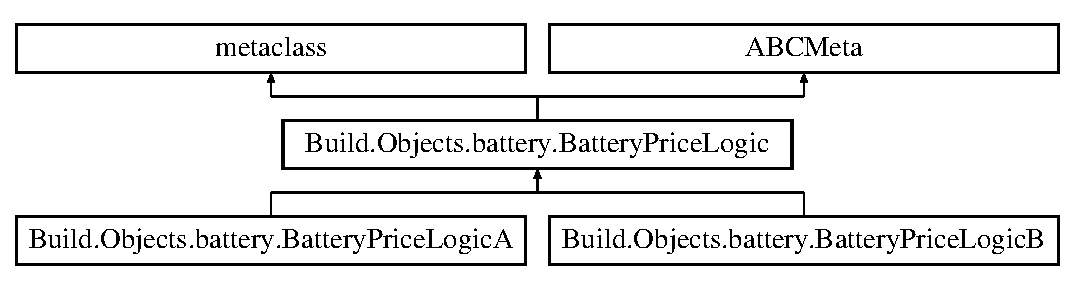
\includegraphics[height=3.000000cm]{class_build_1_1_objects_1_1battery_1_1_battery_price_logic}
\end{center}
\end{figure}
\subsection*{Public Member Functions}
\begin{DoxyCompactItemize}
\item 
def \hyperlink{class_build_1_1_objects_1_1battery_1_1_battery_price_logic_a1a8b8b9981e6bd1cc42d65968cb07c33}{calc\+\_\+charge\+\_\+preference} (self, current\+\_\+soc, current\+\_\+price, price\+\_\+history, average\+\_\+price)
\begin{DoxyCompactList}\small\item\em Determines the charge preference for this battery based on input parameters of current charge, current price, a measure of the price history of the battery for the last 24 hours and/or a total average price. \end{DoxyCompactList}\end{DoxyCompactItemize}


\subsection{Member Function Documentation}
\mbox{\Hypertarget{class_build_1_1_objects_1_1battery_1_1_battery_price_logic_a1a8b8b9981e6bd1cc42d65968cb07c33}\label{class_build_1_1_objects_1_1battery_1_1_battery_price_logic_a1a8b8b9981e6bd1cc42d65968cb07c33}} 
\index{Build\+::\+Objects\+::battery\+::\+Battery\+Price\+Logic@{Build\+::\+Objects\+::battery\+::\+Battery\+Price\+Logic}!calc\+\_\+charge\+\_\+preference@{calc\+\_\+charge\+\_\+preference}}
\index{calc\+\_\+charge\+\_\+preference@{calc\+\_\+charge\+\_\+preference}!Build\+::\+Objects\+::battery\+::\+Battery\+Price\+Logic@{Build\+::\+Objects\+::battery\+::\+Battery\+Price\+Logic}}
\subsubsection{\texorpdfstring{calc\+\_\+charge\+\_\+preference()}{calc\_charge\_preference()}}
{\footnotesize\ttfamily def Build.\+Objects.\+battery.\+Battery\+Price\+Logic.\+calc\+\_\+charge\+\_\+preference (\begin{DoxyParamCaption}\item[{}]{self,  }\item[{}]{current\+\_\+soc,  }\item[{}]{current\+\_\+price,  }\item[{}]{price\+\_\+history,  }\item[{}]{average\+\_\+price }\end{DoxyParamCaption})}



Determines the charge preference for this battery based on input parameters of current charge, current price, a measure of the price history of the battery for the last 24 hours and/or a total average price. 



The documentation for this class was generated from the following file\+:\begin{DoxyCompactItemize}
\item 
Build/\+Objects/battery.\+py\end{DoxyCompactItemize}

\hypertarget{class_build_1_1_objects_1_1battery_1_1_battery_price_logic_a}{}\section{Build.\+Objects.\+battery.\+Battery\+Price\+LogicA Class Reference}
\label{class_build_1_1_objects_1_1battery_1_1_battery_price_logic_a}\index{Build.\+Objects.\+battery.\+Battery\+Price\+LogicA@{Build.\+Objects.\+battery.\+Battery\+Price\+LogicA}}


\hyperlink{class_build_1_1_objects_1_1battery_1_1_battery}{Battery} price logic class which utilizes the average past 24 hourly prices to determine the optimal \char`\"{}threshold price\char`\"{} which influences when a battery prefers to discharge or charge given its current local price.  


Inheritance diagram for Build.\+Objects.\+battery.\+Battery\+Price\+LogicA\+:\begin{figure}[H]
\begin{center}
\leavevmode
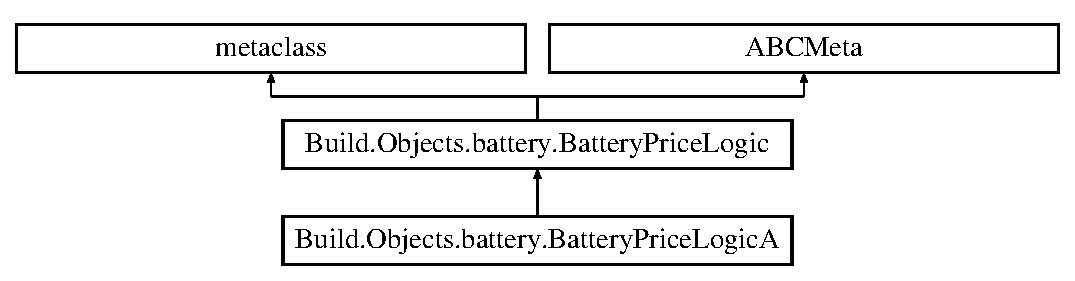
\includegraphics[height=3.000000cm]{class_build_1_1_objects_1_1battery_1_1_battery_price_logic_a}
\end{center}
\end{figure}
\subsection*{Public Member Functions}
\begin{DoxyCompactItemize}
\item 
\mbox{\Hypertarget{class_build_1_1_objects_1_1battery_1_1_battery_price_logic_a_a0134a6435cd19197d759260aef5b7f37}\label{class_build_1_1_objects_1_1battery_1_1_battery_price_logic_a_a0134a6435cd19197d759260aef5b7f37}} 
def {\bfseries \+\_\+\+\_\+init\+\_\+\+\_\+} (self, starting\+\_\+price=0.\+1)
\item 
\mbox{\Hypertarget{class_build_1_1_objects_1_1battery_1_1_battery_price_logic_a_af0520a01ff896c884f8fbdd241c560ab}\label{class_build_1_1_objects_1_1battery_1_1_battery_price_logic_a_af0520a01ff896c884f8fbdd241c560ab}} 
def \hyperlink{class_build_1_1_objects_1_1battery_1_1_battery_price_logic_a_af0520a01ff896c884f8fbdd241c560ab}{calc\+\_\+average\+\_\+price} (self, price\+\_\+history)
\begin{DoxyCompactList}\small\item\em Calculates the average price across the. \end{DoxyCompactList}\item 
def \hyperlink{class_build_1_1_objects_1_1battery_1_1_battery_price_logic_a_a2253d32097370a29c9110248042dbc86}{adjust\+\_\+price\+\_\+thresholds} (self, current\+\_\+soc, price\+\_\+history)
\begin{DoxyCompactList}\small\item\em Method to calculate the price thresholds which help determine the battery\textquotesingle{}s charging preference. \end{DoxyCompactList}\item 
def \hyperlink{class_build_1_1_objects_1_1battery_1_1_battery_price_logic_a_a958d6290df78fa626a89c2ee74c5764b}{calc\+\_\+charge\+\_\+preference} (self, current\+\_\+soc, current\+\_\+price, price\+\_\+history, average\+\_\+price=None)
\begin{DoxyCompactList}\small\item\em Calculates the battery\textquotesingle{}s charging preference based on current price in relation to the calculated price thresholds and absolute charge levels. \end{DoxyCompactList}\end{DoxyCompactItemize}


\subsection{Detailed Description}
\hyperlink{class_build_1_1_objects_1_1battery_1_1_battery}{Battery} price logic class which utilizes the average past 24 hourly prices to determine the optimal \char`\"{}threshold price\char`\"{} which influences when a battery prefers to discharge or charge given its current local price. 



\subsection{Member Function Documentation}
\mbox{\Hypertarget{class_build_1_1_objects_1_1battery_1_1_battery_price_logic_a_a2253d32097370a29c9110248042dbc86}\label{class_build_1_1_objects_1_1battery_1_1_battery_price_logic_a_a2253d32097370a29c9110248042dbc86}} 
\index{Build\+::\+Objects\+::battery\+::\+Battery\+Price\+LogicA@{Build\+::\+Objects\+::battery\+::\+Battery\+Price\+LogicA}!adjust\+\_\+price\+\_\+thresholds@{adjust\+\_\+price\+\_\+thresholds}}
\index{adjust\+\_\+price\+\_\+thresholds@{adjust\+\_\+price\+\_\+thresholds}!Build\+::\+Objects\+::battery\+::\+Battery\+Price\+LogicA@{Build\+::\+Objects\+::battery\+::\+Battery\+Price\+LogicA}}
\subsubsection{\texorpdfstring{adjust\+\_\+price\+\_\+thresholds()}{adjust\_price\_thresholds()}}
{\footnotesize\ttfamily def Build.\+Objects.\+battery.\+Battery\+Price\+Logic\+A.\+adjust\+\_\+price\+\_\+thresholds (\begin{DoxyParamCaption}\item[{}]{self,  }\item[{}]{current\+\_\+soc,  }\item[{}]{price\+\_\+history }\end{DoxyParamCaption})}



Method to calculate the price thresholds which help determine the battery\textquotesingle{}s charging preference. 

Interprets the past 24 hours average price and sets thresholds relative to the minimum, average, and maximum prices. \mbox{\Hypertarget{class_build_1_1_objects_1_1battery_1_1_battery_price_logic_a_a958d6290df78fa626a89c2ee74c5764b}\label{class_build_1_1_objects_1_1battery_1_1_battery_price_logic_a_a958d6290df78fa626a89c2ee74c5764b}} 
\index{Build\+::\+Objects\+::battery\+::\+Battery\+Price\+LogicA@{Build\+::\+Objects\+::battery\+::\+Battery\+Price\+LogicA}!calc\+\_\+charge\+\_\+preference@{calc\+\_\+charge\+\_\+preference}}
\index{calc\+\_\+charge\+\_\+preference@{calc\+\_\+charge\+\_\+preference}!Build\+::\+Objects\+::battery\+::\+Battery\+Price\+LogicA@{Build\+::\+Objects\+::battery\+::\+Battery\+Price\+LogicA}}
\subsubsection{\texorpdfstring{calc\+\_\+charge\+\_\+preference()}{calc\_charge\_preference()}}
{\footnotesize\ttfamily def Build.\+Objects.\+battery.\+Battery\+Price\+Logic\+A.\+calc\+\_\+charge\+\_\+preference (\begin{DoxyParamCaption}\item[{}]{self,  }\item[{}]{current\+\_\+soc,  }\item[{}]{current\+\_\+price,  }\item[{}]{price\+\_\+history,  }\item[{}]{average\+\_\+price = {\ttfamily None} }\end{DoxyParamCaption})}



Calculates the battery\textquotesingle{}s charging preference based on current price in relation to the calculated price thresholds and absolute charge levels. 



The documentation for this class was generated from the following file\+:\begin{DoxyCompactItemize}
\item 
Build/\+Objects/battery.\+py\end{DoxyCompactItemize}

\hypertarget{class_build_1_1_objects_1_1battery_1_1_battery_price_logic_b}{}\section{Build.\+Objects.\+battery.\+Battery\+Price\+LogicB Class Reference}
\label{class_build_1_1_objects_1_1battery_1_1_battery_price_logic_b}\index{Build.\+Objects.\+battery.\+Battery\+Price\+LogicB@{Build.\+Objects.\+battery.\+Battery\+Price\+LogicB}}


\hyperlink{class_build_1_1_objects_1_1battery_1_1_battery}{Battery} price logic class which uses the battery\textquotesingle{}s average price over its entire runtime to determine the desired upper and lower charging thresholds.  


Inheritance diagram for Build.\+Objects.\+battery.\+Battery\+Price\+LogicB\+:\begin{figure}[H]
\begin{center}
\leavevmode
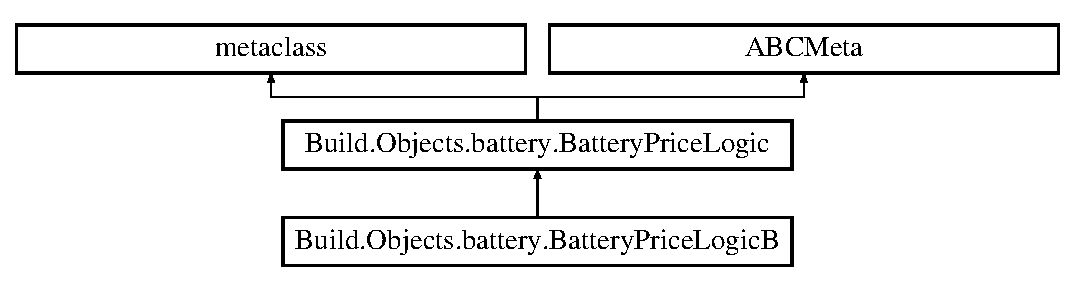
\includegraphics[height=3.000000cm]{class_build_1_1_objects_1_1battery_1_1_battery_price_logic_b}
\end{center}
\end{figure}
\subsection*{Public Member Functions}
\begin{DoxyCompactItemize}
\item 
\mbox{\Hypertarget{class_build_1_1_objects_1_1battery_1_1_battery_price_logic_b_af3b7c19792092798fbbb822cdfa1291d}\label{class_build_1_1_objects_1_1battery_1_1_battery_price_logic_b_af3b7c19792092798fbbb822cdfa1291d}} 
def {\bfseries \+\_\+\+\_\+init\+\_\+\+\_\+} (self, starting\+\_\+price=0.\+1)
\item 
\mbox{\Hypertarget{class_build_1_1_objects_1_1battery_1_1_battery_price_logic_b_a071e4c7da71f4a5aabd385d4a3bb1bb8}\label{class_build_1_1_objects_1_1battery_1_1_battery_price_logic_b_a071e4c7da71f4a5aabd385d4a3bb1bb8}} 
def \hyperlink{class_build_1_1_objects_1_1battery_1_1_battery_price_logic_b_a071e4c7da71f4a5aabd385d4a3bb1bb8}{adjust\+\_\+price\+\_\+thresholds} (self, avg\+\_\+price)
\begin{DoxyCompactList}\small\item\em Sets the thresholds which help determine the battery charging preference, based on direct comparison to the moving average price. \end{DoxyCompactList}\item 
def \hyperlink{class_build_1_1_objects_1_1battery_1_1_battery_price_logic_b_a3b4c1f397cc4ac0d2ae39a7ccc9bccbe}{calc\+\_\+charge\+\_\+preference} (self, current\+\_\+soc, current\+\_\+price, average\+\_\+price, price\+\_\+history=None)
\begin{DoxyCompactList}\small\item\em Calculates the battery\textquotesingle{}s charging preference based on current price in relation to the calculated price thresholds and absolute charge levels. \end{DoxyCompactList}\end{DoxyCompactItemize}


\subsection{Detailed Description}
\hyperlink{class_build_1_1_objects_1_1battery_1_1_battery}{Battery} price logic class which uses the battery\textquotesingle{}s average price over its entire runtime to determine the desired upper and lower charging thresholds. 

\subsection{Member Function Documentation}
\mbox{\Hypertarget{class_build_1_1_objects_1_1battery_1_1_battery_price_logic_b_a3b4c1f397cc4ac0d2ae39a7ccc9bccbe}\label{class_build_1_1_objects_1_1battery_1_1_battery_price_logic_b_a3b4c1f397cc4ac0d2ae39a7ccc9bccbe}} 
\index{Build\+::\+Objects\+::battery\+::\+Battery\+Price\+LogicB@{Build\+::\+Objects\+::battery\+::\+Battery\+Price\+LogicB}!calc\+\_\+charge\+\_\+preference@{calc\+\_\+charge\+\_\+preference}}
\index{calc\+\_\+charge\+\_\+preference@{calc\+\_\+charge\+\_\+preference}!Build\+::\+Objects\+::battery\+::\+Battery\+Price\+LogicB@{Build\+::\+Objects\+::battery\+::\+Battery\+Price\+LogicB}}
\subsubsection{\texorpdfstring{calc\+\_\+charge\+\_\+preference()}{calc\_charge\_preference()}}
{\footnotesize\ttfamily def Build.\+Objects.\+battery.\+Battery\+Price\+Logic\+B.\+calc\+\_\+charge\+\_\+preference (\begin{DoxyParamCaption}\item[{}]{self,  }\item[{}]{current\+\_\+soc,  }\item[{}]{current\+\_\+price,  }\item[{}]{average\+\_\+price,  }\item[{}]{price\+\_\+history = {\ttfamily None} }\end{DoxyParamCaption})}



Calculates the battery\textquotesingle{}s charging preference based on current price in relation to the calculated price thresholds and absolute charge levels. 


\begin{DoxyParams}{Parameters}
{\em price\+\_\+history} & a measure of average price for this battery \\
\hline
\end{DoxyParams}


The documentation for this class was generated from the following file\+:\begin{DoxyCompactItemize}
\item 
Build/\+Objects/battery.\+py\end{DoxyCompactItemize}

\hypertarget{class_build_1_1_objects_1_1device_1_1_device}{}\section{Build.\+Objects.\+device.\+Device Class Reference}
\label{class_build_1_1_objects_1_1device_1_1_device}\index{Build.\+Objects.\+device.\+Device@{Build.\+Objects.\+device.\+Device}}
Inheritance diagram for Build.\+Objects.\+device.\+Device\+:\begin{figure}[H]
\begin{center}
\leavevmode
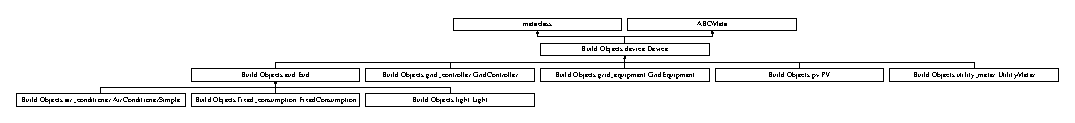
\includegraphics[height=1.204301cm]{class_build_1_1_objects_1_1device_1_1_device}
\end{center}
\end{figure}
\subsection*{Public Member Functions}
\begin{DoxyCompactItemize}
\item 
def \hyperlink{class_build_1_1_objects_1_1device_1_1_device_a6e8b7318d7bce8142f9c482c1852e744}{\+\_\+\+\_\+init\+\_\+\+\_\+} (self, device\+\_\+id, device\+\_\+type, supervisor, time=0, msg\+\_\+latency=0, schedule=None, multiday=0, total\+\_\+runtime=S\+E\+C\+O\+N\+D\+S\+\_\+\+I\+N\+\_\+\+D\+AY, connected\+\_\+devices=None)
\begin{DoxyCompactList}\small\item\em Initialize a device. \end{DoxyCompactList}\item 
def \hyperlink{class_build_1_1_objects_1_1device_1_1_device_a9cf14b880ef9cf103ba68554d3653593}{get\+\_\+id} (self)
\begin{DoxyCompactList}\small\item\em Getter for the \hyperlink{class_build_1_1_objects_1_1device_1_1_device}{Device}\textquotesingle{}s ID We maintain ID as a protected field to avoid external modifications during messaging. \end{DoxyCompactList}\item 
\mbox{\Hypertarget{class_build_1_1_objects_1_1device_1_1_device_a0e0df5ad1dc3572210290c9c613777d4}\label{class_build_1_1_objects_1_1device_1_1_device_a0e0df5ad1dc3572210290c9c613777d4}} 
def \hyperlink{class_build_1_1_objects_1_1device_1_1_device_a0e0df5ad1dc3572210290c9c613777d4}{get\+\_\+type} (self)
\begin{DoxyCompactList}\small\item\em Getter for the \hyperlink{class_build_1_1_objects_1_1device_1_1_device}{Device}\textquotesingle{}s type. \end{DoxyCompactList}\item 
def \hyperlink{class_build_1_1_objects_1_1device_1_1_device_a12de2674ec41c3cfb31689fde187f6e0}{update\+\_\+time} (self, new\+\_\+time)
\begin{DoxyCompactList}\small\item\em Updates the local time of the device. \end{DoxyCompactList}\item 
def \hyperlink{class_build_1_1_objects_1_1device_1_1_device_a1cfab902786e2a6caf3a4b22341e9641}{set\+\_\+power\+\_\+in} (self, power\+\_\+in)
\begin{DoxyCompactList}\small\item\em Sets the power level into the device. \end{DoxyCompactList}\item 
def \hyperlink{class_build_1_1_objects_1_1device_1_1_device_a75d4f47040d95f6e5adb6238cf9e2463}{set\+\_\+power\+\_\+out} (self, power\+\_\+out)
\begin{DoxyCompactList}\small\item\em Sets the power level out of the device. \end{DoxyCompactList}\item 
def \hyperlink{class_build_1_1_objects_1_1device_1_1_device_a576ceef658b74d05291b3dbc2b1ba1da}{recalc\+\_\+sum\+\_\+power} (self, prev\+\_\+power, new\+\_\+power)
\begin{DoxyCompactList}\small\item\em After a device has changed the quantity of power it is sending/receiving, modify the power in and power out. \end{DoxyCompactList}\item 
def \hyperlink{class_build_1_1_objects_1_1device_1_1_device_acbaf978b589fe80b8d4da2f25b266b32}{sum\+\_\+power\+\_\+out} (self)
\begin{DoxyCompactList}\small\item\em Keeps a running total of the energy output by the device Call this method whenever power\+\_\+out level changes. \end{DoxyCompactList}\item 
def \hyperlink{class_build_1_1_objects_1_1device_1_1_device_a6a7287bc43dacb4ab23d04dbd8c01d2f}{sum\+\_\+power\+\_\+in} (self)
\begin{DoxyCompactList}\small\item\em Keeps a running total of the energy consumed by the device Call this method whenever power\+\_\+in level changes. \end{DoxyCompactList}\item 
def \hyperlink{class_build_1_1_objects_1_1device_1_1_device_a8e39400d2e8cf584f912ee9fcccddd2b}{add\+\_\+event} (self, event, time\+\_\+stamp)
\begin{DoxyCompactList}\small\item\em Adds an event to the device\textquotesingle{}s event queue and reports that event to the supervisor Will replace any existing event with the new value. \end{DoxyCompactList}\item 
def \hyperlink{class_build_1_1_objects_1_1device_1_1_device_a49c8b4c3d1c3ca5cc2a070bf6761af8a}{process\+\_\+events} (self)
\begin{DoxyCompactList}\small\item\em Process all events in the device\textquotesingle{}s queue with a given time\+\_\+stamp. \end{DoxyCompactList}\item 
\mbox{\Hypertarget{class_build_1_1_objects_1_1device_1_1_device_ad06156227c33b40f30bcfbc7ae7508b1}\label{class_build_1_1_objects_1_1device_1_1_device_ad06156227c33b40f30bcfbc7ae7508b1}} 
def {\bfseries has\+\_\+upcoming\+\_\+event} (self)
\item 
def \hyperlink{class_build_1_1_objects_1_1device_1_1_device_a5e3fa6ca689529fcf25650e94dcedc62}{report\+\_\+next\+\_\+event\+\_\+time} (self)
\begin{DoxyCompactList}\small\item\em Report the time of the next earliest event in the device\textquotesingle{}s event queue Assumes the event queue is not empty. \end{DoxyCompactList}\item 
def \hyperlink{class_build_1_1_objects_1_1device_1_1_device_a015f4cfeb779c8c6338c65bab7e314ec}{receive\+\_\+message} (self, message)
\begin{DoxyCompactList}\small\item\em Receiving a message is modelled as putting an event with the message a certain delay after the function call. \end{DoxyCompactList}\item 
def \hyperlink{class_build_1_1_objects_1_1device_1_1_device_a65e13b5bb4b33acdd37a084167829056}{read\+\_\+message} (self, message)
\begin{DoxyCompactList}\small\item\em Reads a message and responds based on its message type. \end{DoxyCompactList}\item 
\mbox{\Hypertarget{class_build_1_1_objects_1_1device_1_1_device_afdb3d3a5fc6220f50c025cd0cfed306d}\label{class_build_1_1_objects_1_1device_1_1_device_afdb3d3a5fc6220f50c025cd0cfed306d}} 
def \hyperlink{class_build_1_1_objects_1_1device_1_1_device_afdb3d3a5fc6220f50c025cd0cfed306d}{connect\+\_\+device} (self, wire\+\_\+type, device)
\begin{DoxyCompactList}\small\item\em Connects one device to another. \end{DoxyCompactList}\item 
\mbox{\Hypertarget{class_build_1_1_objects_1_1device_1_1_device_ae349c3bea0d657c805dda47748572dc0}\label{class_build_1_1_objects_1_1device_1_1_device_ae349c3bea0d657c805dda47748572dc0}} 
def {\bfseries disconnect\+\_\+device} (self, device)
\item 
def \hyperlink{class_build_1_1_objects_1_1device_1_1_device_a8ff05d4817a653460ef0873554e3ac87}{register\+\_\+device} (self, device, device\+\_\+id, value)
\begin{DoxyCompactList}\small\item\em Registers or unregisters a given device from the device\textquotesingle{}s connected device list. \end{DoxyCompactList}\item 
def \hyperlink{class_build_1_1_objects_1_1device_1_1_device_ac665d015021b9efa42b734d0cc637304}{process\+\_\+register\+\_\+message} (self, sender\+\_\+id, value)
\begin{DoxyCompactList}\small\item\em Method to be called when the device receives a register message, indicating a device is seeking to register or unregister. \end{DoxyCompactList}\item 
def \hyperlink{class_build_1_1_objects_1_1device_1_1_device_a0acf2d71b9378f7f59e99c1b06c3c23a}{send\+\_\+register\+\_\+message} (self, target\+\_\+id, value)
\begin{DoxyCompactList}\small\item\em Method to be called when the device wants to register or unregister with another device. \end{DoxyCompactList}\item 
def \hyperlink{class_build_1_1_objects_1_1device_1_1_device_a3c71e4e2948f82a8444b2bcb3e6be504}{engage} (self, device\+\_\+list)
\begin{DoxyCompactList}\small\item\em Method to be called when device is entering the grid, and is seeking to register with other devices. \end{DoxyCompactList}\item 
def \hyperlink{class_build_1_1_objects_1_1device_1_1_device_af90a8b21aab7e60dc6ca1dcd7fe00b6f}{process\+\_\+power\+\_\+message} (self, sender\+\_\+id, new\+\_\+power)
\begin{DoxyCompactList}\small\item\em Method to be called when the device receives a power message, indicating power flows have changed between two devices (either receiving or providing). \end{DoxyCompactList}\item 
def \hyperlink{class_build_1_1_objects_1_1device_1_1_device_ab4a83ea60755c15f89dcbff7a10f55cc}{process\+\_\+price\+\_\+message} (self, sender\+\_\+id, new\+\_\+price, extra\+\_\+info)
\begin{DoxyCompactList}\small\item\em Method to be called when device receives a price message. \end{DoxyCompactList}\item 
def \hyperlink{class_build_1_1_objects_1_1device_1_1_device_a83c4bc3f6628bc2ba3343b96c5a441f8}{process\+\_\+request\+\_\+message} (self, sender\+\_\+id, request\+\_\+amt)
\begin{DoxyCompactList}\small\item\em Method to be called when device receives a request message, indicating a device is requesting to either provide or receive the requested quantity of power. \end{DoxyCompactList}\item 
def \hyperlink{class_build_1_1_objects_1_1device_1_1_device_af80aeef7fa18bef428cb622fc9d23d2c}{process\+\_\+allocate\+\_\+message} (self, sender\+\_\+id, allocate\+\_\+amt)
\begin{DoxyCompactList}\small\item\em Method to be called once device has allocated to provide a given quantity of power to another device, or to receive a given quantity of power. \end{DoxyCompactList}\item 
def \hyperlink{class_build_1_1_objects_1_1device_1_1_device_a06ffd25b07e6361e4ecb1e3432cff477}{setup\+\_\+schedule} (self, scheduled\+\_\+events, runtime=S\+E\+C\+O\+N\+D\+S\+\_\+\+I\+N\+\_\+\+D\+AY, multiday=0)
\item 
def \hyperlink{class_build_1_1_objects_1_1device_1_1_device_a94094fa08f506cd2f02e0d4a9611153d}{build\+\_\+log\+\_\+notation} (self, message=\char`\"{}\char`\"{}, tag=\char`\"{}\char`\"{}, value=None)
\begin{DoxyCompactList}\small\item\em Builds a logging message from a message, tag, and value, which also includes time and device\+\_\+id. \end{DoxyCompactList}\item 
def \hyperlink{class_build_1_1_objects_1_1device_1_1_device_aff92b20a263ce0f7a715789305ca0d30}{write\+\_\+calcs} (self)
\begin{DoxyCompactList}\small\item\em Writes the calculations of total energy in and out of this device in wH to the log file then writes any other calculations specific to the device-\/type. \end{DoxyCompactList}\item 
\mbox{\Hypertarget{class_build_1_1_objects_1_1device_1_1_device_a1027097a4c8bedb6abf9d52f41e194f9}\label{class_build_1_1_objects_1_1device_1_1_device_a1027097a4c8bedb6abf9d52f41e194f9}} 
def \hyperlink{class_build_1_1_objects_1_1device_1_1_device_a1027097a4c8bedb6abf9d52f41e194f9}{device\+\_\+specific\+\_\+calcs} (self)
\begin{DoxyCompactList}\small\item\em All device specific power consumption/runtime statistics are added here. \end{DoxyCompactList}\item 
def \hyperlink{class_build_1_1_objects_1_1device_1_1_device_a0eb251de12fe74493c71a50713b5ac3a}{finish} (self, end\+\_\+time)
\begin{DoxyCompactList}\small\item\em Method to be called at end of simulation resetting power levels and calculating end\+\_\+time the time to update the local time to. \end{DoxyCompactList}\end{DoxyCompactItemize}


\subsection{Constructor \& Destructor Documentation}
\mbox{\Hypertarget{class_build_1_1_objects_1_1device_1_1_device_a6e8b7318d7bce8142f9c482c1852e744}\label{class_build_1_1_objects_1_1device_1_1_device_a6e8b7318d7bce8142f9c482c1852e744}} 
\index{Build\+::\+Objects\+::device\+::\+Device@{Build\+::\+Objects\+::device\+::\+Device}!\+\_\+\+\_\+init\+\_\+\+\_\+@{\+\_\+\+\_\+init\+\_\+\+\_\+}}
\index{\+\_\+\+\_\+init\+\_\+\+\_\+@{\+\_\+\+\_\+init\+\_\+\+\_\+}!Build\+::\+Objects\+::device\+::\+Device@{Build\+::\+Objects\+::device\+::\+Device}}
\subsubsection{\texorpdfstring{\+\_\+\+\_\+init\+\_\+\+\_\+()}{\_\_init\_\_()}}
{\footnotesize\ttfamily def Build.\+Objects.\+device.\+Device.\+\_\+\+\_\+init\+\_\+\+\_\+ (\begin{DoxyParamCaption}\item[{}]{self,  }\item[{}]{device\+\_\+id,  }\item[{}]{device\+\_\+type,  }\item[{}]{supervisor,  }\item[{}]{time = {\ttfamily 0},  }\item[{}]{msg\+\_\+latency = {\ttfamily 0},  }\item[{}]{schedule = {\ttfamily None},  }\item[{}]{multiday = {\ttfamily 0},  }\item[{}]{total\+\_\+runtime = {\ttfamily SECONDS\+\_\+IN\+\_\+DAY},  }\item[{}]{connected\+\_\+devices = {\ttfamily None} }\end{DoxyParamCaption})}



Initialize a device. 


\begin{DoxyParams}{Parameters}
{\em device\+\_\+id} & unique device ID. Must begin with type of device (see documentation). \\
\hline
{\em device\+\_\+type} & the type of this device (the most specific class descriptor) \\
\hline
{\em uuid} & the device\textquotesingle{}s emergency shutdown priority \\
\hline
{\em time} & device\textquotesingle{}s local time, in seconds. This will be updated by the supervisor. \\
\hline
{\em msg\+\_\+latency} & the delay time before this device processes a received message. \\
\hline
{\em connected\+\_\+devices} & a list of the names of connected devices for this device. \\
\hline
\end{DoxyParams}


\subsection{Member Function Documentation}
\mbox{\Hypertarget{class_build_1_1_objects_1_1device_1_1_device_a8e39400d2e8cf584f912ee9fcccddd2b}\label{class_build_1_1_objects_1_1device_1_1_device_a8e39400d2e8cf584f912ee9fcccddd2b}} 
\index{Build\+::\+Objects\+::device\+::\+Device@{Build\+::\+Objects\+::device\+::\+Device}!add\+\_\+event@{add\+\_\+event}}
\index{add\+\_\+event@{add\+\_\+event}!Build\+::\+Objects\+::device\+::\+Device@{Build\+::\+Objects\+::device\+::\+Device}}
\subsubsection{\texorpdfstring{add\+\_\+event()}{add\_event()}}
{\footnotesize\ttfamily def Build.\+Objects.\+device.\+Device.\+add\+\_\+event (\begin{DoxyParamCaption}\item[{}]{self,  }\item[{}]{event,  }\item[{}]{time\+\_\+stamp }\end{DoxyParamCaption})}



Adds an event to the device\textquotesingle{}s event queue and reports that event to the supervisor Will replace any existing event with the new value. 

Hence, only one event type at a time 
\begin{DoxyParams}{Parameters}
{\em event} & the event to add to the event queue \\
\hline
{\em time\+\_\+stamp} & the time to associate with the event in the queue \\
\hline
\end{DoxyParams}
\mbox{\Hypertarget{class_build_1_1_objects_1_1device_1_1_device_a94094fa08f506cd2f02e0d4a9611153d}\label{class_build_1_1_objects_1_1device_1_1_device_a94094fa08f506cd2f02e0d4a9611153d}} 
\index{Build\+::\+Objects\+::device\+::\+Device@{Build\+::\+Objects\+::device\+::\+Device}!build\+\_\+log\+\_\+notation@{build\+\_\+log\+\_\+notation}}
\index{build\+\_\+log\+\_\+notation@{build\+\_\+log\+\_\+notation}!Build\+::\+Objects\+::device\+::\+Device@{Build\+::\+Objects\+::device\+::\+Device}}
\subsubsection{\texorpdfstring{build\+\_\+log\+\_\+notation()}{build\_log\_notation()}}
{\footnotesize\ttfamily def Build.\+Objects.\+device.\+Device.\+build\+\_\+log\+\_\+notation (\begin{DoxyParamCaption}\item[{}]{self,  }\item[{}]{message = {\ttfamily \char`\"{}\char`\"{}},  }\item[{}]{tag = {\ttfamily \char`\"{}\char`\"{}},  }\item[{}]{value = {\ttfamily None} }\end{DoxyParamCaption})}



Builds a logging message from a message, tag, and value, which also includes time and device\+\_\+id. 


\begin{DoxyParams}{Parameters}
{\em message} & the message to add to logger \\
\hline
{\em tag} & the tag to associate with this message to add to the logger \\
\hline
{\em value} & the value for this message to add to the logger \\
\hline
\end{DoxyParams}
\mbox{\Hypertarget{class_build_1_1_objects_1_1device_1_1_device_a3c71e4e2948f82a8444b2bcb3e6be504}\label{class_build_1_1_objects_1_1device_1_1_device_a3c71e4e2948f82a8444b2bcb3e6be504}} 
\index{Build\+::\+Objects\+::device\+::\+Device@{Build\+::\+Objects\+::device\+::\+Device}!engage@{engage}}
\index{engage@{engage}!Build\+::\+Objects\+::device\+::\+Device@{Build\+::\+Objects\+::device\+::\+Device}}
\subsubsection{\texorpdfstring{engage()}{engage()}}
{\footnotesize\ttfamily def Build.\+Objects.\+device.\+Device.\+engage (\begin{DoxyParamCaption}\item[{}]{self,  }\item[{}]{device\+\_\+list }\end{DoxyParamCaption})}



Method to be called when device is entering the grid, and is seeking to register with other devices. 


\begin{DoxyParams}{Parameters}
{\em device\+\_\+list} & the connected list of devices to add to its connected device list and to inform it has registered. Must be devices themselves (not ID\textquotesingle{}s). \\
\hline
\end{DoxyParams}
\mbox{\Hypertarget{class_build_1_1_objects_1_1device_1_1_device_a0eb251de12fe74493c71a50713b5ac3a}\label{class_build_1_1_objects_1_1device_1_1_device_a0eb251de12fe74493c71a50713b5ac3a}} 
\index{Build\+::\+Objects\+::device\+::\+Device@{Build\+::\+Objects\+::device\+::\+Device}!finish@{finish}}
\index{finish@{finish}!Build\+::\+Objects\+::device\+::\+Device@{Build\+::\+Objects\+::device\+::\+Device}}
\subsubsection{\texorpdfstring{finish()}{finish()}}
{\footnotesize\ttfamily def Build.\+Objects.\+device.\+Device.\+finish (\begin{DoxyParamCaption}\item[{}]{self,  }\item[{}]{end\+\_\+time }\end{DoxyParamCaption})}



Method to be called at end of simulation resetting power levels and calculating end\+\_\+time the time to update the local time to. 

\begin{DoxyVerb}"Gets called at the end of the simulation\end{DoxyVerb}
 \mbox{\Hypertarget{class_build_1_1_objects_1_1device_1_1_device_a9cf14b880ef9cf103ba68554d3653593}\label{class_build_1_1_objects_1_1device_1_1_device_a9cf14b880ef9cf103ba68554d3653593}} 
\index{Build\+::\+Objects\+::device\+::\+Device@{Build\+::\+Objects\+::device\+::\+Device}!get\+\_\+id@{get\+\_\+id}}
\index{get\+\_\+id@{get\+\_\+id}!Build\+::\+Objects\+::device\+::\+Device@{Build\+::\+Objects\+::device\+::\+Device}}
\subsubsection{\texorpdfstring{get\+\_\+id()}{get\_id()}}
{\footnotesize\ttfamily def Build.\+Objects.\+device.\+Device.\+get\+\_\+id (\begin{DoxyParamCaption}\item[{}]{self }\end{DoxyParamCaption})}



Getter for the \hyperlink{class_build_1_1_objects_1_1device_1_1_device}{Device}\textquotesingle{}s ID We maintain ID as a protected field to avoid external modifications during messaging. 

\begin{DoxyReturn}{Returns}
the device\textquotesingle{}s ID 
\end{DoxyReturn}
\mbox{\Hypertarget{class_build_1_1_objects_1_1device_1_1_device_af80aeef7fa18bef428cb622fc9d23d2c}\label{class_build_1_1_objects_1_1device_1_1_device_af80aeef7fa18bef428cb622fc9d23d2c}} 
\index{Build\+::\+Objects\+::device\+::\+Device@{Build\+::\+Objects\+::device\+::\+Device}!process\+\_\+allocate\+\_\+message@{process\+\_\+allocate\+\_\+message}}
\index{process\+\_\+allocate\+\_\+message@{process\+\_\+allocate\+\_\+message}!Build\+::\+Objects\+::device\+::\+Device@{Build\+::\+Objects\+::device\+::\+Device}}
\subsubsection{\texorpdfstring{process\+\_\+allocate\+\_\+message()}{process\_allocate\_message()}}
{\footnotesize\ttfamily def Build.\+Objects.\+device.\+Device.\+process\+\_\+allocate\+\_\+message (\begin{DoxyParamCaption}\item[{}]{self,  }\item[{}]{sender\+\_\+id,  }\item[{}]{allocate\+\_\+amt }\end{DoxyParamCaption})}



Method to be called once device has allocated to provide a given quantity of power to another device, or to receive a given quantity of power. 

Allocation should only ever occur after request messages have been passed and processed.


\begin{DoxyParams}{Parameters}
{\em allocated\+\_\+amt} & the amount this device has been allocated to receive (must be positive). \\
\hline
\end{DoxyParams}
\mbox{\Hypertarget{class_build_1_1_objects_1_1device_1_1_device_a49c8b4c3d1c3ca5cc2a070bf6761af8a}\label{class_build_1_1_objects_1_1device_1_1_device_a49c8b4c3d1c3ca5cc2a070bf6761af8a}} 
\index{Build\+::\+Objects\+::device\+::\+Device@{Build\+::\+Objects\+::device\+::\+Device}!process\+\_\+events@{process\+\_\+events}}
\index{process\+\_\+events@{process\+\_\+events}!Build\+::\+Objects\+::device\+::\+Device@{Build\+::\+Objects\+::device\+::\+Device}}
\subsubsection{\texorpdfstring{process\+\_\+events()}{process\_events()}}
{\footnotesize\ttfamily def Build.\+Objects.\+device.\+Device.\+process\+\_\+events (\begin{DoxyParamCaption}\item[{}]{self }\end{DoxyParamCaption})}



Process all events in the device\textquotesingle{}s queue with a given time\+\_\+stamp. 

This function should be called after advance\+\_\+time has been called by the supervisor. \mbox{\Hypertarget{class_build_1_1_objects_1_1device_1_1_device_af90a8b21aab7e60dc6ca1dcd7fe00b6f}\label{class_build_1_1_objects_1_1device_1_1_device_af90a8b21aab7e60dc6ca1dcd7fe00b6f}} 
\index{Build\+::\+Objects\+::device\+::\+Device@{Build\+::\+Objects\+::device\+::\+Device}!process\+\_\+power\+\_\+message@{process\+\_\+power\+\_\+message}}
\index{process\+\_\+power\+\_\+message@{process\+\_\+power\+\_\+message}!Build\+::\+Objects\+::device\+::\+Device@{Build\+::\+Objects\+::device\+::\+Device}}
\subsubsection{\texorpdfstring{process\+\_\+power\+\_\+message()}{process\_power\_message()}}
{\footnotesize\ttfamily def Build.\+Objects.\+device.\+Device.\+process\+\_\+power\+\_\+message (\begin{DoxyParamCaption}\item[{}]{self,  }\item[{}]{sender\+\_\+id,  }\item[{}]{new\+\_\+power }\end{DoxyParamCaption})}



Method to be called when the device receives a power message, indicating power flows have changed between two devices (either receiving or providing). 


\begin{DoxyParams}{Parameters}
{\em sender} & the sender of the message providing or receiving the new power \\
\hline
{\em new\+\_\+power} & the value of power flow from sender\textquotesingle{}s perspective positive if sender is receiving, negative if sender is providing. \\
\hline
\end{DoxyParams}
\mbox{\Hypertarget{class_build_1_1_objects_1_1device_1_1_device_ab4a83ea60755c15f89dcbff7a10f55cc}\label{class_build_1_1_objects_1_1device_1_1_device_ab4a83ea60755c15f89dcbff7a10f55cc}} 
\index{Build\+::\+Objects\+::device\+::\+Device@{Build\+::\+Objects\+::device\+::\+Device}!process\+\_\+price\+\_\+message@{process\+\_\+price\+\_\+message}}
\index{process\+\_\+price\+\_\+message@{process\+\_\+price\+\_\+message}!Build\+::\+Objects\+::device\+::\+Device@{Build\+::\+Objects\+::device\+::\+Device}}
\subsubsection{\texorpdfstring{process\+\_\+price\+\_\+message()}{process\_price\_message()}}
{\footnotesize\ttfamily def Build.\+Objects.\+device.\+Device.\+process\+\_\+price\+\_\+message (\begin{DoxyParamCaption}\item[{}]{self,  }\item[{}]{sender\+\_\+id,  }\item[{}]{new\+\_\+price,  }\item[{}]{extra\+\_\+info }\end{DoxyParamCaption})}



Method to be called when device receives a price message. 


\begin{DoxyParams}{Parameters}
{\em sender\+\_\+id} & the sender of the message informing of the new price \\
\hline
{\em new\+\_\+price} & the new price value \\
\hline
{\em extra\+\_\+info} & additional information contained in this price message. From the utility meter, this is its buy prices, from other devices this can be price forecast information. \\
\hline
\end{DoxyParams}
\mbox{\Hypertarget{class_build_1_1_objects_1_1device_1_1_device_ac665d015021b9efa42b734d0cc637304}\label{class_build_1_1_objects_1_1device_1_1_device_ac665d015021b9efa42b734d0cc637304}} 
\index{Build\+::\+Objects\+::device\+::\+Device@{Build\+::\+Objects\+::device\+::\+Device}!process\+\_\+register\+\_\+message@{process\+\_\+register\+\_\+message}}
\index{process\+\_\+register\+\_\+message@{process\+\_\+register\+\_\+message}!Build\+::\+Objects\+::device\+::\+Device@{Build\+::\+Objects\+::device\+::\+Device}}
\subsubsection{\texorpdfstring{process\+\_\+register\+\_\+message()}{process\_register\_message()}}
{\footnotesize\ttfamily def Build.\+Objects.\+device.\+Device.\+process\+\_\+register\+\_\+message (\begin{DoxyParamCaption}\item[{}]{self,  }\item[{}]{sender\+\_\+id,  }\item[{}]{value }\end{DoxyParamCaption})}



Method to be called when the device receives a register message, indicating a device is seeking to register or unregister. 


\begin{DoxyParams}{Parameters}
{\em sender} & the sender of the message informing of registering. \\
\hline
{\em value} & positive if sender is registering negative if unregistering \\
\hline
\end{DoxyParams}
\mbox{\Hypertarget{class_build_1_1_objects_1_1device_1_1_device_a83c4bc3f6628bc2ba3343b96c5a441f8}\label{class_build_1_1_objects_1_1device_1_1_device_a83c4bc3f6628bc2ba3343b96c5a441f8}} 
\index{Build\+::\+Objects\+::device\+::\+Device@{Build\+::\+Objects\+::device\+::\+Device}!process\+\_\+request\+\_\+message@{process\+\_\+request\+\_\+message}}
\index{process\+\_\+request\+\_\+message@{process\+\_\+request\+\_\+message}!Build\+::\+Objects\+::device\+::\+Device@{Build\+::\+Objects\+::device\+::\+Device}}
\subsubsection{\texorpdfstring{process\+\_\+request\+\_\+message()}{process\_request\_message()}}
{\footnotesize\ttfamily def Build.\+Objects.\+device.\+Device.\+process\+\_\+request\+\_\+message (\begin{DoxyParamCaption}\item[{}]{self,  }\item[{}]{sender\+\_\+id,  }\item[{}]{request\+\_\+amt }\end{DoxyParamCaption})}



Method to be called when device receives a request message, indicating a device is requesting to either provide or receive the requested quantity of power. 


\begin{DoxyParams}{Parameters}
{\em request\+\_\+amt} & the amount the sending device is requesting to receive (must be positive) \\
\hline
\end{DoxyParams}
\mbox{\Hypertarget{class_build_1_1_objects_1_1device_1_1_device_a65e13b5bb4b33acdd37a084167829056}\label{class_build_1_1_objects_1_1device_1_1_device_a65e13b5bb4b33acdd37a084167829056}} 
\index{Build\+::\+Objects\+::device\+::\+Device@{Build\+::\+Objects\+::device\+::\+Device}!read\+\_\+message@{read\+\_\+message}}
\index{read\+\_\+message@{read\+\_\+message}!Build\+::\+Objects\+::device\+::\+Device@{Build\+::\+Objects\+::device\+::\+Device}}
\subsubsection{\texorpdfstring{read\+\_\+message()}{read\_message()}}
{\footnotesize\ttfamily def Build.\+Objects.\+device.\+Device.\+read\+\_\+message (\begin{DoxyParamCaption}\item[{}]{self,  }\item[{}]{message }\end{DoxyParamCaption})}



Reads a message and responds based on its message type. 


\begin{DoxyParams}{Parameters}
{\em message} & a message to be read (must be a message object) \\
\hline
\end{DoxyParams}
\mbox{\Hypertarget{class_build_1_1_objects_1_1device_1_1_device_a576ceef658b74d05291b3dbc2b1ba1da}\label{class_build_1_1_objects_1_1device_1_1_device_a576ceef658b74d05291b3dbc2b1ba1da}} 
\index{Build\+::\+Objects\+::device\+::\+Device@{Build\+::\+Objects\+::device\+::\+Device}!recalc\+\_\+sum\+\_\+power@{recalc\+\_\+sum\+\_\+power}}
\index{recalc\+\_\+sum\+\_\+power@{recalc\+\_\+sum\+\_\+power}!Build\+::\+Objects\+::device\+::\+Device@{Build\+::\+Objects\+::device\+::\+Device}}
\subsubsection{\texorpdfstring{recalc\+\_\+sum\+\_\+power()}{recalc\_sum\_power()}}
{\footnotesize\ttfamily def Build.\+Objects.\+device.\+Device.\+recalc\+\_\+sum\+\_\+power (\begin{DoxyParamCaption}\item[{}]{self,  }\item[{}]{prev\+\_\+power,  }\item[{}]{new\+\_\+power }\end{DoxyParamCaption})}



After a device has changed the quantity of power it is sending/receiving, modify the power in and power out. 

Call whenever a load has been changed on this device. 
\begin{DoxyParams}{Parameters}
{\em prev\+\_\+power} & the previous power flow from this device\textquotesingle{}s perspective (in positive, out negative) \\
\hline
{\em new\+\_\+power} & the new power flow from this device\textquotesingle{}s perspective (in positive, out negative) \\
\hline
\end{DoxyParams}
\mbox{\Hypertarget{class_build_1_1_objects_1_1device_1_1_device_a015f4cfeb779c8c6338c65bab7e314ec}\label{class_build_1_1_objects_1_1device_1_1_device_a015f4cfeb779c8c6338c65bab7e314ec}} 
\index{Build\+::\+Objects\+::device\+::\+Device@{Build\+::\+Objects\+::device\+::\+Device}!receive\+\_\+message@{receive\+\_\+message}}
\index{receive\+\_\+message@{receive\+\_\+message}!Build\+::\+Objects\+::device\+::\+Device@{Build\+::\+Objects\+::device\+::\+Device}}
\subsubsection{\texorpdfstring{receive\+\_\+message()}{receive\_message()}}
{\footnotesize\ttfamily def Build.\+Objects.\+device.\+Device.\+receive\+\_\+message (\begin{DoxyParamCaption}\item[{}]{self,  }\item[{}]{message }\end{DoxyParamCaption})}



Receiving a message is modelled as putting an event with the message a certain delay after the function call. 


\begin{DoxyParams}{Parameters}
{\em message} & the message to receive. \\
\hline
\end{DoxyParams}
\mbox{\Hypertarget{class_build_1_1_objects_1_1device_1_1_device_a8ff05d4817a653460ef0873554e3ac87}\label{class_build_1_1_objects_1_1device_1_1_device_a8ff05d4817a653460ef0873554e3ac87}} 
\index{Build\+::\+Objects\+::device\+::\+Device@{Build\+::\+Objects\+::device\+::\+Device}!register\+\_\+device@{register\+\_\+device}}
\index{register\+\_\+device@{register\+\_\+device}!Build\+::\+Objects\+::device\+::\+Device@{Build\+::\+Objects\+::device\+::\+Device}}
\subsubsection{\texorpdfstring{register\+\_\+device()}{register\_device()}}
{\footnotesize\ttfamily def Build.\+Objects.\+device.\+Device.\+register\+\_\+device (\begin{DoxyParamCaption}\item[{}]{self,  }\item[{}]{device,  }\item[{}]{device\+\_\+id,  }\item[{}]{value }\end{DoxyParamCaption})}



Registers or unregisters a given device from the device\textquotesingle{}s connected device list. 


\begin{DoxyParams}{Parameters}
{\em device} & the device to register or unregister from connected devices \\
\hline
{\em that} & device\textquotesingle{}s id \\
\hline
{\em value} & positive to register, 0 or negative to unregister \\
\hline
\end{DoxyParams}
\mbox{\Hypertarget{class_build_1_1_objects_1_1device_1_1_device_a5e3fa6ca689529fcf25650e94dcedc62}\label{class_build_1_1_objects_1_1device_1_1_device_a5e3fa6ca689529fcf25650e94dcedc62}} 
\index{Build\+::\+Objects\+::device\+::\+Device@{Build\+::\+Objects\+::device\+::\+Device}!report\+\_\+next\+\_\+event\+\_\+time@{report\+\_\+next\+\_\+event\+\_\+time}}
\index{report\+\_\+next\+\_\+event\+\_\+time@{report\+\_\+next\+\_\+event\+\_\+time}!Build\+::\+Objects\+::device\+::\+Device@{Build\+::\+Objects\+::device\+::\+Device}}
\subsubsection{\texorpdfstring{report\+\_\+next\+\_\+event\+\_\+time()}{report\_next\_event\_time()}}
{\footnotesize\ttfamily def Build.\+Objects.\+device.\+Device.\+report\+\_\+next\+\_\+event\+\_\+time (\begin{DoxyParamCaption}\item[{}]{self }\end{DoxyParamCaption})}



Report the time of the next earliest event in the device\textquotesingle{}s event queue Assumes the event queue is not empty. 

Call has\+\_\+upcoming\+\_\+event first. \begin{DoxyReturn}{Returns}
a tuple of device\textquotesingle{}s ID and the time of its next event 
\end{DoxyReturn}
\mbox{\Hypertarget{class_build_1_1_objects_1_1device_1_1_device_a0acf2d71b9378f7f59e99c1b06c3c23a}\label{class_build_1_1_objects_1_1device_1_1_device_a0acf2d71b9378f7f59e99c1b06c3c23a}} 
\index{Build\+::\+Objects\+::device\+::\+Device@{Build\+::\+Objects\+::device\+::\+Device}!send\+\_\+register\+\_\+message@{send\+\_\+register\+\_\+message}}
\index{send\+\_\+register\+\_\+message@{send\+\_\+register\+\_\+message}!Build\+::\+Objects\+::device\+::\+Device@{Build\+::\+Objects\+::device\+::\+Device}}
\subsubsection{\texorpdfstring{send\+\_\+register\+\_\+message()}{send\_register\_message()}}
{\footnotesize\ttfamily def Build.\+Objects.\+device.\+Device.\+send\+\_\+register\+\_\+message (\begin{DoxyParamCaption}\item[{}]{self,  }\item[{}]{target\+\_\+id,  }\item[{}]{value }\end{DoxyParamCaption})}



Method to be called when the device wants to register or unregister with another device. 


\begin{DoxyParams}{Parameters}
{\em target\+\_\+id} & the device to receive the register message \\
\hline
{\em value} & positive if registering negative if unregistering \\
\hline
\end{DoxyParams}
\mbox{\Hypertarget{class_build_1_1_objects_1_1device_1_1_device_a1cfab902786e2a6caf3a4b22341e9641}\label{class_build_1_1_objects_1_1device_1_1_device_a1cfab902786e2a6caf3a4b22341e9641}} 
\index{Build\+::\+Objects\+::device\+::\+Device@{Build\+::\+Objects\+::device\+::\+Device}!set\+\_\+power\+\_\+in@{set\+\_\+power\+\_\+in}}
\index{set\+\_\+power\+\_\+in@{set\+\_\+power\+\_\+in}!Build\+::\+Objects\+::device\+::\+Device@{Build\+::\+Objects\+::device\+::\+Device}}
\subsubsection{\texorpdfstring{set\+\_\+power\+\_\+in()}{set\_power\_in()}}
{\footnotesize\ttfamily def Build.\+Objects.\+device.\+Device.\+set\+\_\+power\+\_\+in (\begin{DoxyParamCaption}\item[{}]{self,  }\item[{}]{power\+\_\+in }\end{DoxyParamCaption})}



Sets the power level into the device. 

Call this method when setting absolute power levels e.\+g. turning the device off


\begin{DoxyParams}{Parameters}
{\em power\+\_\+in} & the new amount of power in to device (non-\/negative). \\
\hline
\end{DoxyParams}
\mbox{\Hypertarget{class_build_1_1_objects_1_1device_1_1_device_a75d4f47040d95f6e5adb6238cf9e2463}\label{class_build_1_1_objects_1_1device_1_1_device_a75d4f47040d95f6e5adb6238cf9e2463}} 
\index{Build\+::\+Objects\+::device\+::\+Device@{Build\+::\+Objects\+::device\+::\+Device}!set\+\_\+power\+\_\+out@{set\+\_\+power\+\_\+out}}
\index{set\+\_\+power\+\_\+out@{set\+\_\+power\+\_\+out}!Build\+::\+Objects\+::device\+::\+Device@{Build\+::\+Objects\+::device\+::\+Device}}
\subsubsection{\texorpdfstring{set\+\_\+power\+\_\+out()}{set\_power\_out()}}
{\footnotesize\ttfamily def Build.\+Objects.\+device.\+Device.\+set\+\_\+power\+\_\+out (\begin{DoxyParamCaption}\item[{}]{self,  }\item[{}]{power\+\_\+out }\end{DoxyParamCaption})}



Sets the power level out of the device. 

Call this method when setting absolute power levels e.\+g. turning the device off


\begin{DoxyParams}{Parameters}
{\em power\+\_\+in} & the new amount of power in to device (non-\/negative). \\
\hline
\end{DoxyParams}
\mbox{\Hypertarget{class_build_1_1_objects_1_1device_1_1_device_a06ffd25b07e6361e4ecb1e3432cff477}\label{class_build_1_1_objects_1_1device_1_1_device_a06ffd25b07e6361e4ecb1e3432cff477}} 
\index{Build\+::\+Objects\+::device\+::\+Device@{Build\+::\+Objects\+::device\+::\+Device}!setup\+\_\+schedule@{setup\+\_\+schedule}}
\index{setup\+\_\+schedule@{setup\+\_\+schedule}!Build\+::\+Objects\+::device\+::\+Device@{Build\+::\+Objects\+::device\+::\+Device}}
\subsubsection{\texorpdfstring{setup\+\_\+schedule()}{setup\_schedule()}}
{\footnotesize\ttfamily def Build.\+Objects.\+device.\+Device.\+setup\+\_\+schedule (\begin{DoxyParamCaption}\item[{}]{self,  }\item[{}]{scheduled\+\_\+events,  }\item[{}]{runtime = {\ttfamily SECONDS\+\_\+IN\+\_\+DAY},  }\item[{}]{multiday = {\ttfamily 0} }\end{DoxyParamCaption})}


\begin{DoxyParams}{Parameters}
{\em a} & list of scheduled events to add to the device\textquotesingle{}s queue, in the format of list of list of time(seconds), operation\+\_\+name \\
\hline
\end{DoxyParams}
\mbox{\Hypertarget{class_build_1_1_objects_1_1device_1_1_device_a6a7287bc43dacb4ab23d04dbd8c01d2f}\label{class_build_1_1_objects_1_1device_1_1_device_a6a7287bc43dacb4ab23d04dbd8c01d2f}} 
\index{Build\+::\+Objects\+::device\+::\+Device@{Build\+::\+Objects\+::device\+::\+Device}!sum\+\_\+power\+\_\+in@{sum\+\_\+power\+\_\+in}}
\index{sum\+\_\+power\+\_\+in@{sum\+\_\+power\+\_\+in}!Build\+::\+Objects\+::device\+::\+Device@{Build\+::\+Objects\+::device\+::\+Device}}
\subsubsection{\texorpdfstring{sum\+\_\+power\+\_\+in()}{sum\_power\_in()}}
{\footnotesize\ttfamily def Build.\+Objects.\+device.\+Device.\+sum\+\_\+power\+\_\+in (\begin{DoxyParamCaption}\item[{}]{self }\end{DoxyParamCaption})}



Keeps a running total of the energy consumed by the device Call this method whenever power\+\_\+in level changes. 

\mbox{\Hypertarget{class_build_1_1_objects_1_1device_1_1_device_acbaf978b589fe80b8d4da2f25b266b32}\label{class_build_1_1_objects_1_1device_1_1_device_acbaf978b589fe80b8d4da2f25b266b32}} 
\index{Build\+::\+Objects\+::device\+::\+Device@{Build\+::\+Objects\+::device\+::\+Device}!sum\+\_\+power\+\_\+out@{sum\+\_\+power\+\_\+out}}
\index{sum\+\_\+power\+\_\+out@{sum\+\_\+power\+\_\+out}!Build\+::\+Objects\+::device\+::\+Device@{Build\+::\+Objects\+::device\+::\+Device}}
\subsubsection{\texorpdfstring{sum\+\_\+power\+\_\+out()}{sum\_power\_out()}}
{\footnotesize\ttfamily def Build.\+Objects.\+device.\+Device.\+sum\+\_\+power\+\_\+out (\begin{DoxyParamCaption}\item[{}]{self }\end{DoxyParamCaption})}



Keeps a running total of the energy output by the device Call this method whenever power\+\_\+out level changes. 

\mbox{\Hypertarget{class_build_1_1_objects_1_1device_1_1_device_a12de2674ec41c3cfb31689fde187f6e0}\label{class_build_1_1_objects_1_1device_1_1_device_a12de2674ec41c3cfb31689fde187f6e0}} 
\index{Build\+::\+Objects\+::device\+::\+Device@{Build\+::\+Objects\+::device\+::\+Device}!update\+\_\+time@{update\+\_\+time}}
\index{update\+\_\+time@{update\+\_\+time}!Build\+::\+Objects\+::device\+::\+Device@{Build\+::\+Objects\+::device\+::\+Device}}
\subsubsection{\texorpdfstring{update\+\_\+time()}{update\_time()}}
{\footnotesize\ttfamily def Build.\+Objects.\+device.\+Device.\+update\+\_\+time (\begin{DoxyParamCaption}\item[{}]{self,  }\item[{}]{new\+\_\+time }\end{DoxyParamCaption})}



Updates the local time of the device. 

This method is only called by the Supervisor once it is about to process a next initial event. 
\begin{DoxyParams}{Parameters}
{\em new\+\_\+time} & the time to update to \\
\hline
\end{DoxyParams}
\mbox{\Hypertarget{class_build_1_1_objects_1_1device_1_1_device_aff92b20a263ce0f7a715789305ca0d30}\label{class_build_1_1_objects_1_1device_1_1_device_aff92b20a263ce0f7a715789305ca0d30}} 
\index{Build\+::\+Objects\+::device\+::\+Device@{Build\+::\+Objects\+::device\+::\+Device}!write\+\_\+calcs@{write\+\_\+calcs}}
\index{write\+\_\+calcs@{write\+\_\+calcs}!Build\+::\+Objects\+::device\+::\+Device@{Build\+::\+Objects\+::device\+::\+Device}}
\subsubsection{\texorpdfstring{write\+\_\+calcs()}{write\_calcs()}}
{\footnotesize\ttfamily def Build.\+Objects.\+device.\+Device.\+write\+\_\+calcs (\begin{DoxyParamCaption}\item[{}]{self }\end{DoxyParamCaption})}



Writes the calculations of total energy in and out of this device in wH to the log file then writes any other calculations specific to the device-\/type. 



The documentation for this class was generated from the following file\+:\begin{DoxyCompactItemize}
\item 
Build/\+Objects/device.\+py\end{DoxyCompactItemize}

\hypertarget{class_build_1_1_objects_1_1eud_1_1_eud}{}\section{Build.\+Objects.\+eud.\+Eud Class Reference}
\label{class_build_1_1_objects_1_1eud_1_1_eud}\index{Build.\+Objects.\+eud.\+Eud@{Build.\+Objects.\+eud.\+Eud}}
Inheritance diagram for Build.\+Objects.\+eud.\+Eud\+:\begin{figure}[H]
\begin{center}
\leavevmode
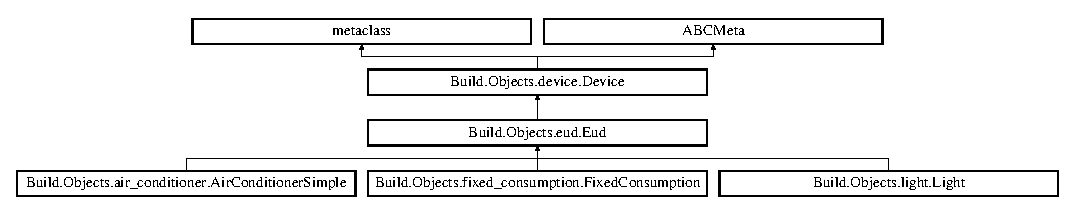
\includegraphics[height=2.408602cm]{class_build_1_1_objects_1_1eud_1_1_eud}
\end{center}
\end{figure}
\subsection*{Public Member Functions}
\begin{DoxyCompactItemize}
\item 
\mbox{\Hypertarget{class_build_1_1_objects_1_1eud_1_1_eud_ae9a2bace7d3af75a2a0746ab6ea9103c}\label{class_build_1_1_objects_1_1eud_1_1_eud_ae9a2bace7d3af75a2a0746ab6ea9103c}} 
def {\bfseries \+\_\+\+\_\+init\+\_\+\+\_\+} (self, device\+\_\+id, device\+\_\+type, supervisor, total\+\_\+runtime, time=0, msg\+\_\+latency=0, power\+\_\+direct=False, modulation\+\_\+interval=600, schedule=None, multiday=0, connected\+\_\+devices=None)
\item 
def \hyperlink{class_build_1_1_objects_1_1eud_1_1_eud_a8601f950b8b11f28f9ec0e80965c8b25}{start\+\_\+up} (self)
\begin{DoxyCompactList}\small\item\em Turns on the E\+UD, seeking to update to its desired power level. \end{DoxyCompactList}\item 
def \hyperlink{class_build_1_1_objects_1_1eud_1_1_eud_afc9354486371abba2f70e6a1605459e3}{shut\+\_\+down} (self)
\begin{DoxyCompactList}\small\item\em Turns off the E\+UD. \end{DoxyCompactList}\item 
\mbox{\Hypertarget{class_build_1_1_objects_1_1eud_1_1_eud_a7a4ea640840f7c33015a204d83cc0b59}\label{class_build_1_1_objects_1_1eud_1_1_eud_a7a4ea640840f7c33015a204d83cc0b59}} 
def \hyperlink{class_build_1_1_objects_1_1eud_1_1_eud_a7a4ea640840f7c33015a204d83cc0b59}{set\+\_\+allocated} (self, device\+\_\+id, allocate\+\_\+amt)
\begin{DoxyCompactList}\small\item\em Sets the quantity of power that this E\+UD has been allocated to consume by a specific device. \end{DoxyCompactList}\item 
def \hyperlink{class_build_1_1_objects_1_1eud_1_1_eud_a6f7982b4d798f0a26222ec4a96366b9a}{setup\+\_\+modulation\+\_\+schedule} (self, modulation\+\_\+interval, total\+\_\+runtime)
\begin{DoxyCompactList}\small\item\em The E\+UD will modulate its power every 10 minutes. \end{DoxyCompactList}\item 
def \hyperlink{class_build_1_1_objects_1_1eud_1_1_eud_a5105203c22df5b2e9c1754b8889563df}{process\+\_\+power\+\_\+message} (self, sender\+\_\+id, new\+\_\+power)
\begin{DoxyCompactList}\small\item\em Method to be called when this E\+UD receives a power message. \end{DoxyCompactList}\item 
def \hyperlink{class_build_1_1_objects_1_1eud_1_1_eud_a4e9b1ca4c510a1f405f5d16b31215cbe}{process\+\_\+request\+\_\+message} (self, sender\+\_\+id, request\+\_\+amt)
\begin{DoxyCompactList}\small\item\em E\+UD\textquotesingle{}s do not respond to request messages. \end{DoxyCompactList}\item 
def \hyperlink{class_build_1_1_objects_1_1eud_1_1_eud_abef38cebc5b66f6cb03f58f2900b9a93}{process\+\_\+price\+\_\+message} (self, sender\+\_\+id, new\+\_\+price, extra\+\_\+info)
\begin{DoxyCompactList}\small\item\em Method to be called after the E\+UD receives a price message from a grid controller, immediately updating its price. \end{DoxyCompactList}\item 
def \hyperlink{class_build_1_1_objects_1_1eud_1_1_eud_af02e4338062f37389c04e87d9d5f9f63}{process\+\_\+allocate\+\_\+message} (self, sender\+\_\+id, allocate\+\_\+amt)
\begin{DoxyCompactList}\small\item\em Method to be called once device has allocated to provide a given quantity of power to another device, or to receive a given quantity of power. \end{DoxyCompactList}\item 
def \hyperlink{class_build_1_1_objects_1_1eud_1_1_eud_a13b6abd062b9b88597dc83c9c7813fdc}{send\+\_\+request\+\_\+message} (self, target\+\_\+id, request\+\_\+amt)
\begin{DoxyCompactList}\small\item\em This method is called when the E\+UD is requesting to use power from a GC. \end{DoxyCompactList}\item 
\mbox{\Hypertarget{class_build_1_1_objects_1_1eud_1_1_eud_a45a3f08a0d82e961c9244f54fe446608}\label{class_build_1_1_objects_1_1eud_1_1_eud_a45a3f08a0d82e961c9244f54fe446608}} 
def {\bfseries send\+\_\+power\+\_\+message} (self, target\+\_\+id, power\+\_\+amt)
\item 
\mbox{\Hypertarget{class_build_1_1_objects_1_1eud_1_1_eud_a652d92e9486fef78851127b876b000ff}\label{class_build_1_1_objects_1_1eud_1_1_eud_a652d92e9486fef78851127b876b000ff}} 
def {\bfseries change\+\_\+load\+\_\+in} (self, sender\+\_\+id, new\+\_\+load)
\item 
def \hyperlink{class_build_1_1_objects_1_1eud_1_1_eud_a11d57b7f91d22bd696f2b29a8ac93044}{modulate\+\_\+power} (self)
\begin{DoxyCompactList}\small\item\em Method to be called once it needs to recalculate its internal power usage. \end{DoxyCompactList}\item 
\mbox{\Hypertarget{class_build_1_1_objects_1_1eud_1_1_eud_a0a75866bd7e1478fa1f459bfb0da6675}\label{class_build_1_1_objects_1_1eud_1_1_eud_a0a75866bd7e1478fa1f459bfb0da6675}} 
def {\bfseries begin\+\_\+internal\+\_\+operation} (self)
\item 
\mbox{\Hypertarget{class_build_1_1_objects_1_1eud_1_1_eud_a82b817dc748e1b5db87f4e47755b64ec}\label{class_build_1_1_objects_1_1eud_1_1_eud_a82b817dc748e1b5db87f4e47755b64ec}} 
def \hyperlink{class_build_1_1_objects_1_1eud_1_1_eud_a82b817dc748e1b5db87f4e47755b64ec}{end\+\_\+internal\+\_\+operation} (self)
\begin{DoxyCompactList}\small\item\em \hyperlink{class_build_1_1_objects_1_1eud_1_1_eud}{Eud} specific processes to initiate or terminate when this device turns off. \end{DoxyCompactList}\item 
def \hyperlink{class_build_1_1_objects_1_1eud_1_1_eud_a690ec54ec92b3d2373858fe460013730}{calculate\+\_\+desired\+\_\+power\+\_\+level} (self)
\begin{DoxyCompactList}\small\item\em Calculates E\+UD\textquotesingle{}s desired power in to support its current internal state levels. \end{DoxyCompactList}\item 
def \hyperlink{class_build_1_1_objects_1_1eud_1_1_eud_a89a88154fdd5e8a4c9c1207eb3cb3f2f}{respond\+\_\+to\+\_\+power} (self, received\+\_\+power)
\begin{DoxyCompactList}\small\item\em How this E\+UD responds once it receives a given quantity of power after requesting a certain amount. \end{DoxyCompactList}\item 
def \hyperlink{class_build_1_1_objects_1_1eud_1_1_eud_ac807e57f20360c9e828046a38aaa7db6}{update\+\_\+state} (self)
\begin{DoxyCompactList}\small\item\em Call to update all the internal state functions of the E\+UD. \end{DoxyCompactList}\item 
def \hyperlink{class_build_1_1_objects_1_1eud_1_1_eud_a4d6c3c842206a1738efd24319ddc2176}{device\+\_\+specific\+\_\+calcs} (self)
\begin{DoxyCompactList}\small\item\em All device specific end-\/of-\/simulation calculations are E\+U\+D-\/specific. \end{DoxyCompactList}\end{DoxyCompactItemize}
\subsection*{Public Attributes}
\begin{DoxyCompactItemize}
\item 
\mbox{\Hypertarget{class_build_1_1_objects_1_1eud_1_1_eud_a79c2171714e8f604f2cf6e1b245dcf9f}\label{class_build_1_1_objects_1_1eud_1_1_eud_a79c2171714e8f604f2cf6e1b245dcf9f}} 
{\bfseries power\+\_\+recalibration\+\_\+interval}
\item 
\mbox{\Hypertarget{class_build_1_1_objects_1_1eud_1_1_eud_ad35f5cbe19da59af227b7a38c4b76ae9}\label{class_build_1_1_objects_1_1eud_1_1_eud_ad35f5cbe19da59af227b7a38c4b76ae9}} 
{\bfseries price\+\_\+recalibration\+\_\+interval}
\end{DoxyCompactItemize}


\subsection{Member Function Documentation}
\mbox{\Hypertarget{class_build_1_1_objects_1_1eud_1_1_eud_a690ec54ec92b3d2373858fe460013730}\label{class_build_1_1_objects_1_1eud_1_1_eud_a690ec54ec92b3d2373858fe460013730}} 
\index{Build\+::\+Objects\+::eud\+::\+Eud@{Build\+::\+Objects\+::eud\+::\+Eud}!calculate\+\_\+desired\+\_\+power\+\_\+level@{calculate\+\_\+desired\+\_\+power\+\_\+level}}
\index{calculate\+\_\+desired\+\_\+power\+\_\+level@{calculate\+\_\+desired\+\_\+power\+\_\+level}!Build\+::\+Objects\+::eud\+::\+Eud@{Build\+::\+Objects\+::eud\+::\+Eud}}
\subsubsection{\texorpdfstring{calculate\+\_\+desired\+\_\+power\+\_\+level()}{calculate\_desired\_power\_level()}}
{\footnotesize\ttfamily def Build.\+Objects.\+eud.\+Eud.\+calculate\+\_\+desired\+\_\+power\+\_\+level (\begin{DoxyParamCaption}\item[{}]{self }\end{DoxyParamCaption})}



Calculates E\+UD\textquotesingle{}s desired power in to support its current internal state levels. 

N\+O\+TE\+: E\+UD must be in\+\_\+operation for this function to work. \begin{DoxyReturn}{Returns}
the eud\textquotesingle{}s desired power in 
\end{DoxyReturn}
\mbox{\Hypertarget{class_build_1_1_objects_1_1eud_1_1_eud_a4d6c3c842206a1738efd24319ddc2176}\label{class_build_1_1_objects_1_1eud_1_1_eud_a4d6c3c842206a1738efd24319ddc2176}} 
\index{Build\+::\+Objects\+::eud\+::\+Eud@{Build\+::\+Objects\+::eud\+::\+Eud}!device\+\_\+specific\+\_\+calcs@{device\+\_\+specific\+\_\+calcs}}
\index{device\+\_\+specific\+\_\+calcs@{device\+\_\+specific\+\_\+calcs}!Build\+::\+Objects\+::eud\+::\+Eud@{Build\+::\+Objects\+::eud\+::\+Eud}}
\subsubsection{\texorpdfstring{device\+\_\+specific\+\_\+calcs()}{device\_specific\_calcs()}}
{\footnotesize\ttfamily def Build.\+Objects.\+eud.\+Eud.\+device\+\_\+specific\+\_\+calcs (\begin{DoxyParamCaption}\item[{}]{self }\end{DoxyParamCaption})}



All device specific end-\/of-\/simulation calculations are E\+U\+D-\/specific. 

\mbox{\Hypertarget{class_build_1_1_objects_1_1eud_1_1_eud_a11d57b7f91d22bd696f2b29a8ac93044}\label{class_build_1_1_objects_1_1eud_1_1_eud_a11d57b7f91d22bd696f2b29a8ac93044}} 
\index{Build\+::\+Objects\+::eud\+::\+Eud@{Build\+::\+Objects\+::eud\+::\+Eud}!modulate\+\_\+power@{modulate\+\_\+power}}
\index{modulate\+\_\+power@{modulate\+\_\+power}!Build\+::\+Objects\+::eud\+::\+Eud@{Build\+::\+Objects\+::eud\+::\+Eud}}
\subsubsection{\texorpdfstring{modulate\+\_\+power()}{modulate\_power()}}
{\footnotesize\ttfamily def Build.\+Objects.\+eud.\+Eud.\+modulate\+\_\+power (\begin{DoxyParamCaption}\item[{}]{self }\end{DoxyParamCaption})}



Method to be called once it needs to recalculate its internal power usage. 

To be called after price, power level, or allocate has changed. This function will change the E\+UD\textquotesingle{}s power level to the desired level. This function is compatible with this E\+UD being associated with multiple grid controllers. E\+UD specific processes to initiate when this device turns on \mbox{\Hypertarget{class_build_1_1_objects_1_1eud_1_1_eud_af02e4338062f37389c04e87d9d5f9f63}\label{class_build_1_1_objects_1_1eud_1_1_eud_af02e4338062f37389c04e87d9d5f9f63}} 
\index{Build\+::\+Objects\+::eud\+::\+Eud@{Build\+::\+Objects\+::eud\+::\+Eud}!process\+\_\+allocate\+\_\+message@{process\+\_\+allocate\+\_\+message}}
\index{process\+\_\+allocate\+\_\+message@{process\+\_\+allocate\+\_\+message}!Build\+::\+Objects\+::eud\+::\+Eud@{Build\+::\+Objects\+::eud\+::\+Eud}}
\subsubsection{\texorpdfstring{process\+\_\+allocate\+\_\+message()}{process\_allocate\_message()}}
{\footnotesize\ttfamily def Build.\+Objects.\+eud.\+Eud.\+process\+\_\+allocate\+\_\+message (\begin{DoxyParamCaption}\item[{}]{self,  }\item[{}]{sender\+\_\+id,  }\item[{}]{allocate\+\_\+amt }\end{DoxyParamCaption})}



Method to be called once device has allocated to provide a given quantity of power to another device, or to receive a given quantity of power. 


\begin{DoxyParams}{Parameters}
{\em sender\+\_\+id} & the device who has allocated to provide the given quantity \\
\hline
{\em allocated\+\_\+amt} & the amount that the sending device has allocated to receive from this E\+UD. Hence, this E\+UD cannot respond unless the value is negative, since the E\+UD only consumes power. \\
\hline
\end{DoxyParams}
\mbox{\Hypertarget{class_build_1_1_objects_1_1eud_1_1_eud_a5105203c22df5b2e9c1754b8889563df}\label{class_build_1_1_objects_1_1eud_1_1_eud_a5105203c22df5b2e9c1754b8889563df}} 
\index{Build\+::\+Objects\+::eud\+::\+Eud@{Build\+::\+Objects\+::eud\+::\+Eud}!process\+\_\+power\+\_\+message@{process\+\_\+power\+\_\+message}}
\index{process\+\_\+power\+\_\+message@{process\+\_\+power\+\_\+message}!Build\+::\+Objects\+::eud\+::\+Eud@{Build\+::\+Objects\+::eud\+::\+Eud}}
\subsubsection{\texorpdfstring{process\+\_\+power\+\_\+message()}{process\_power\_message()}}
{\footnotesize\ttfamily def Build.\+Objects.\+eud.\+Eud.\+process\+\_\+power\+\_\+message (\begin{DoxyParamCaption}\item[{}]{self,  }\item[{}]{sender\+\_\+id,  }\item[{}]{new\+\_\+power }\end{DoxyParamCaption})}



Method to be called when this E\+UD receives a power message. 

If there is an erroneous message suggesting for the E\+UD to provide power, it immediately responds with a \char`\"{}0\char`\"{} price message. 
\begin{DoxyParams}{Parameters}
{\em sender\+\_\+id} & the sender of the power message \\
\hline
{\em new\+\_\+power} & the new power value from the sender\textquotesingle{}s perspective \\
\hline
\end{DoxyParams}
\mbox{\Hypertarget{class_build_1_1_objects_1_1eud_1_1_eud_abef38cebc5b66f6cb03f58f2900b9a93}\label{class_build_1_1_objects_1_1eud_1_1_eud_abef38cebc5b66f6cb03f58f2900b9a93}} 
\index{Build\+::\+Objects\+::eud\+::\+Eud@{Build\+::\+Objects\+::eud\+::\+Eud}!process\+\_\+price\+\_\+message@{process\+\_\+price\+\_\+message}}
\index{process\+\_\+price\+\_\+message@{process\+\_\+price\+\_\+message}!Build\+::\+Objects\+::eud\+::\+Eud@{Build\+::\+Objects\+::eud\+::\+Eud}}
\subsubsection{\texorpdfstring{process\+\_\+price\+\_\+message()}{process\_price\_message()}}
{\footnotesize\ttfamily def Build.\+Objects.\+eud.\+Eud.\+process\+\_\+price\+\_\+message (\begin{DoxyParamCaption}\item[{}]{self,  }\item[{}]{sender\+\_\+id,  }\item[{}]{new\+\_\+price,  }\item[{}]{extra\+\_\+info }\end{DoxyParamCaption})}



Method to be called after the E\+UD receives a price message from a grid controller, immediately updating its price. 

\mbox{\Hypertarget{class_build_1_1_objects_1_1eud_1_1_eud_a4e9b1ca4c510a1f405f5d16b31215cbe}\label{class_build_1_1_objects_1_1eud_1_1_eud_a4e9b1ca4c510a1f405f5d16b31215cbe}} 
\index{Build\+::\+Objects\+::eud\+::\+Eud@{Build\+::\+Objects\+::eud\+::\+Eud}!process\+\_\+request\+\_\+message@{process\+\_\+request\+\_\+message}}
\index{process\+\_\+request\+\_\+message@{process\+\_\+request\+\_\+message}!Build\+::\+Objects\+::eud\+::\+Eud@{Build\+::\+Objects\+::eud\+::\+Eud}}
\subsubsection{\texorpdfstring{process\+\_\+request\+\_\+message()}{process\_request\_message()}}
{\footnotesize\ttfamily def Build.\+Objects.\+eud.\+Eud.\+process\+\_\+request\+\_\+message (\begin{DoxyParamCaption}\item[{}]{self,  }\item[{}]{sender\+\_\+id,  }\item[{}]{request\+\_\+amt }\end{DoxyParamCaption})}



E\+UD\textquotesingle{}s do not respond to request messages. 

\mbox{\Hypertarget{class_build_1_1_objects_1_1eud_1_1_eud_a89a88154fdd5e8a4c9c1207eb3cb3f2f}\label{class_build_1_1_objects_1_1eud_1_1_eud_a89a88154fdd5e8a4c9c1207eb3cb3f2f}} 
\index{Build\+::\+Objects\+::eud\+::\+Eud@{Build\+::\+Objects\+::eud\+::\+Eud}!respond\+\_\+to\+\_\+power@{respond\+\_\+to\+\_\+power}}
\index{respond\+\_\+to\+\_\+power@{respond\+\_\+to\+\_\+power}!Build\+::\+Objects\+::eud\+::\+Eud@{Build\+::\+Objects\+::eud\+::\+Eud}}
\subsubsection{\texorpdfstring{respond\+\_\+to\+\_\+power()}{respond\_to\_power()}}
{\footnotesize\ttfamily def Build.\+Objects.\+eud.\+Eud.\+respond\+\_\+to\+\_\+power (\begin{DoxyParamCaption}\item[{}]{self,  }\item[{}]{received\+\_\+power }\end{DoxyParamCaption})}



How this E\+UD responds once it receives a given quantity of power after requesting a certain amount. 


\begin{DoxyParams}{Parameters}
{\em received\+\_\+power} & how much power this device immediately received (must be positive value) \\
\hline
\end{DoxyParams}
\mbox{\Hypertarget{class_build_1_1_objects_1_1eud_1_1_eud_a13b6abd062b9b88597dc83c9c7813fdc}\label{class_build_1_1_objects_1_1eud_1_1_eud_a13b6abd062b9b88597dc83c9c7813fdc}} 
\index{Build\+::\+Objects\+::eud\+::\+Eud@{Build\+::\+Objects\+::eud\+::\+Eud}!send\+\_\+request\+\_\+message@{send\+\_\+request\+\_\+message}}
\index{send\+\_\+request\+\_\+message@{send\+\_\+request\+\_\+message}!Build\+::\+Objects\+::eud\+::\+Eud@{Build\+::\+Objects\+::eud\+::\+Eud}}
\subsubsection{\texorpdfstring{send\+\_\+request\+\_\+message()}{send\_request\_message()}}
{\footnotesize\ttfamily def Build.\+Objects.\+eud.\+Eud.\+send\+\_\+request\+\_\+message (\begin{DoxyParamCaption}\item[{}]{self,  }\item[{}]{target\+\_\+id,  }\item[{}]{request\+\_\+amt }\end{DoxyParamCaption})}



This method is called when the E\+UD is requesting to use power from a GC. 


\begin{DoxyParams}{Parameters}
{\em target\+\_\+id} & the recipient of the request message (must be a GC) \\
\hline
{\em request\+\_\+amt} & the amount of power this E\+UD is requesting to receive (must be positive) \\
\hline
\end{DoxyParams}
\mbox{\Hypertarget{class_build_1_1_objects_1_1eud_1_1_eud_a6f7982b4d798f0a26222ec4a96366b9a}\label{class_build_1_1_objects_1_1eud_1_1_eud_a6f7982b4d798f0a26222ec4a96366b9a}} 
\index{Build\+::\+Objects\+::eud\+::\+Eud@{Build\+::\+Objects\+::eud\+::\+Eud}!setup\+\_\+modulation\+\_\+schedule@{setup\+\_\+modulation\+\_\+schedule}}
\index{setup\+\_\+modulation\+\_\+schedule@{setup\+\_\+modulation\+\_\+schedule}!Build\+::\+Objects\+::eud\+::\+Eud@{Build\+::\+Objects\+::eud\+::\+Eud}}
\subsubsection{\texorpdfstring{setup\+\_\+modulation\+\_\+schedule()}{setup\_modulation\_schedule()}}
{\footnotesize\ttfamily def Build.\+Objects.\+eud.\+Eud.\+setup\+\_\+modulation\+\_\+schedule (\begin{DoxyParamCaption}\item[{}]{self,  }\item[{}]{modulation\+\_\+interval,  }\item[{}]{total\+\_\+runtime }\end{DoxyParamCaption})}



The E\+UD will modulate its power every 10 minutes. 

\mbox{\Hypertarget{class_build_1_1_objects_1_1eud_1_1_eud_afc9354486371abba2f70e6a1605459e3}\label{class_build_1_1_objects_1_1eud_1_1_eud_afc9354486371abba2f70e6a1605459e3}} 
\index{Build\+::\+Objects\+::eud\+::\+Eud@{Build\+::\+Objects\+::eud\+::\+Eud}!shut\+\_\+down@{shut\+\_\+down}}
\index{shut\+\_\+down@{shut\+\_\+down}!Build\+::\+Objects\+::eud\+::\+Eud@{Build\+::\+Objects\+::eud\+::\+Eud}}
\subsubsection{\texorpdfstring{shut\+\_\+down()}{shut\_down()}}
{\footnotesize\ttfamily def Build.\+Objects.\+eud.\+Eud.\+shut\+\_\+down (\begin{DoxyParamCaption}\item[{}]{self }\end{DoxyParamCaption})}



Turns off the E\+UD. 

Reduces all power consumption to 0 and informs all connected grid controllers of this change. \mbox{\Hypertarget{class_build_1_1_objects_1_1eud_1_1_eud_a8601f950b8b11f28f9ec0e80965c8b25}\label{class_build_1_1_objects_1_1eud_1_1_eud_a8601f950b8b11f28f9ec0e80965c8b25}} 
\index{Build\+::\+Objects\+::eud\+::\+Eud@{Build\+::\+Objects\+::eud\+::\+Eud}!start\+\_\+up@{start\+\_\+up}}
\index{start\+\_\+up@{start\+\_\+up}!Build\+::\+Objects\+::eud\+::\+Eud@{Build\+::\+Objects\+::eud\+::\+Eud}}
\subsubsection{\texorpdfstring{start\+\_\+up()}{start\_up()}}
{\footnotesize\ttfamily def Build.\+Objects.\+eud.\+Eud.\+start\+\_\+up (\begin{DoxyParamCaption}\item[{}]{self }\end{DoxyParamCaption})}



Turns on the E\+UD, seeking to update to its desired power level. 

Previous state functions such as price are maintained. If E\+UD is already on, does not do anything. \mbox{\Hypertarget{class_build_1_1_objects_1_1eud_1_1_eud_ac807e57f20360c9e828046a38aaa7db6}\label{class_build_1_1_objects_1_1eud_1_1_eud_ac807e57f20360c9e828046a38aaa7db6}} 
\index{Build\+::\+Objects\+::eud\+::\+Eud@{Build\+::\+Objects\+::eud\+::\+Eud}!update\+\_\+state@{update\+\_\+state}}
\index{update\+\_\+state@{update\+\_\+state}!Build\+::\+Objects\+::eud\+::\+Eud@{Build\+::\+Objects\+::eud\+::\+Eud}}
\subsubsection{\texorpdfstring{update\+\_\+state()}{update\_state()}}
{\footnotesize\ttfamily def Build.\+Objects.\+eud.\+Eud.\+update\+\_\+state (\begin{DoxyParamCaption}\item[{}]{self }\end{DoxyParamCaption})}



Call to update all the internal state functions of the E\+UD. 

Call this function before calling calculate desired power level. 

The documentation for this class was generated from the following file\+:\begin{DoxyCompactItemize}
\item 
Build/\+Objects/eud.\+py\end{DoxyCompactItemize}

\hypertarget{class_build_1_1_simulation___operation_1_1event_1_1_event}{}\section{Build.\+Simulation\+\_\+\+Operation.\+event.\+Event Class Reference}
\label{class_build_1_1_simulation___operation_1_1event_1_1_event}\index{Build.\+Simulation\+\_\+\+Operation.\+event.\+Event@{Build.\+Simulation\+\_\+\+Operation.\+event.\+Event}}


$\ast$$\ast$$\ast$ Copyright Notice $\ast$$\ast$$\ast$  


Inheritance diagram for Build.\+Simulation\+\_\+\+Operation.\+event.\+Event\+:\begin{figure}[H]
\begin{center}
\leavevmode
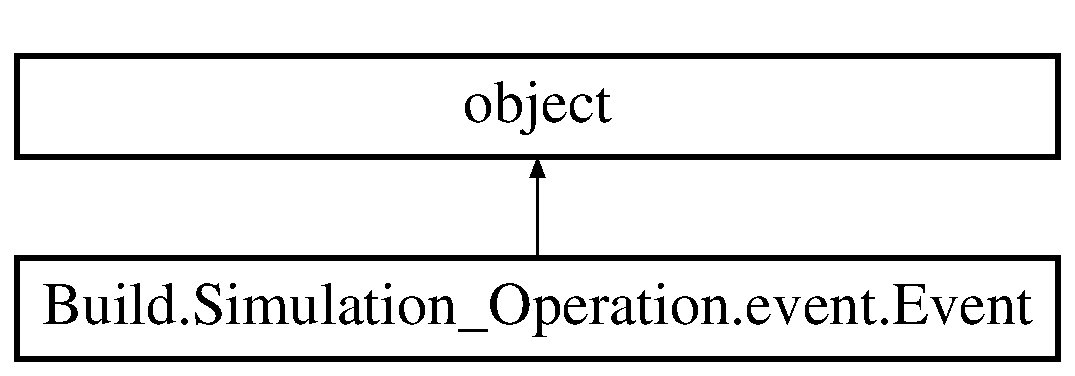
\includegraphics[height=2.000000cm]{class_build_1_1_simulation___operation_1_1event_1_1_event}
\end{center}
\end{figure}
\subsection*{Public Member Functions}
\begin{DoxyCompactItemize}
\item 
def \hyperlink{class_build_1_1_simulation___operation_1_1event_1_1_event_a9453491fff56e3d46eff942d308d4c87}{\+\_\+\+\_\+init\+\_\+\+\_\+} (self, action, args)
\begin{DoxyCompactList}\small\item\em Initialize an event with a function and arguments for that function. \end{DoxyCompactList}\item 
def \hyperlink{class_build_1_1_simulation___operation_1_1event_1_1_event_a0714e3275d4c67cd5e1757e846fc3dbf}{run\+\_\+event} (self)
\begin{DoxyCompactList}\small\item\em Initialize an event with a function and arguments for that function. \end{DoxyCompactList}\end{DoxyCompactItemize}


\subsection{Detailed Description}
$\ast$$\ast$$\ast$ Copyright Notice $\ast$$\ast$$\ast$ 

\char`\"{}\+Price Based Local Power Distribution Management System (\+Local Power Distribution Manager) v2.\+0\char`\"{} Copyright (c) 2017, The Regents of the University of California, through Lawrence Berkeley National Laboratory (subject to receipt of any required approvals from the U.\+S. Dept. of Energy). All rights reserved.

If you have questions about your rights to use or distribute this software, please contact Berkeley Lab\textquotesingle{}s Innovation \& Partnerships Office at \href{mailto:IPO@lbl.gov}{\tt I\+P\+O@lbl.\+gov}. 

\subsection{Constructor \& Destructor Documentation}
\mbox{\Hypertarget{class_build_1_1_simulation___operation_1_1event_1_1_event_a9453491fff56e3d46eff942d308d4c87}\label{class_build_1_1_simulation___operation_1_1event_1_1_event_a9453491fff56e3d46eff942d308d4c87}} 
\index{Build\+::\+Simulation\+\_\+\+Operation\+::event\+::\+Event@{Build\+::\+Simulation\+\_\+\+Operation\+::event\+::\+Event}!\+\_\+\+\_\+init\+\_\+\+\_\+@{\+\_\+\+\_\+init\+\_\+\+\_\+}}
\index{\+\_\+\+\_\+init\+\_\+\+\_\+@{\+\_\+\+\_\+init\+\_\+\+\_\+}!Build\+::\+Simulation\+\_\+\+Operation\+::event\+::\+Event@{Build\+::\+Simulation\+\_\+\+Operation\+::event\+::\+Event}}
\subsubsection{\texorpdfstring{\+\_\+\+\_\+init\+\_\+\+\_\+()}{\_\_init\_\_()}}
{\footnotesize\ttfamily def Build.\+Simulation\+\_\+\+Operation.\+event.\+Event.\+\_\+\+\_\+init\+\_\+\+\_\+ (\begin{DoxyParamCaption}\item[{}]{self,  }\item[{}]{action,  }\item[{}]{args }\end{DoxyParamCaption})}



Initialize an event with a function and arguments for that function. 


\begin{DoxyParams}{Parameters}
{\em action} & a state-\/affecting function to be run in the event (function does not return a value). \\
\hline
{\em args} & any number of arguments to pass into the function to pack into a tuple. \\
\hline
\end{DoxyParams}


\subsection{Member Function Documentation}
\mbox{\Hypertarget{class_build_1_1_simulation___operation_1_1event_1_1_event_a0714e3275d4c67cd5e1757e846fc3dbf}\label{class_build_1_1_simulation___operation_1_1event_1_1_event_a0714e3275d4c67cd5e1757e846fc3dbf}} 
\index{Build\+::\+Simulation\+\_\+\+Operation\+::event\+::\+Event@{Build\+::\+Simulation\+\_\+\+Operation\+::event\+::\+Event}!run\+\_\+event@{run\+\_\+event}}
\index{run\+\_\+event@{run\+\_\+event}!Build\+::\+Simulation\+\_\+\+Operation\+::event\+::\+Event@{Build\+::\+Simulation\+\_\+\+Operation\+::event\+::\+Event}}
\subsubsection{\texorpdfstring{run\+\_\+event()}{run\_event()}}
{\footnotesize\ttfamily def Build.\+Simulation\+\_\+\+Operation.\+event.\+Event.\+run\+\_\+event (\begin{DoxyParamCaption}\item[{}]{self }\end{DoxyParamCaption})}



Initialize an event with a function and arguments for that function. 


\begin{DoxyParams}{Parameters}
{\em action} & a function to be run in the event \\
\hline
{\em args} & a tuple of arguments for the function \\
\hline
\end{DoxyParams}


The documentation for this class was generated from the following file\+:\begin{DoxyCompactItemize}
\item 
Build/\+Simulation\+\_\+\+Operation/event.\+py\end{DoxyCompactItemize}

\hypertarget{class_build_1_1_objects_1_1fixed__consumption_1_1_fixed_consumption}{}\section{Build.\+Objects.\+fixed\+\_\+consumption.\+Fixed\+Consumption Class Reference}
\label{class_build_1_1_objects_1_1fixed__consumption_1_1_fixed_consumption}\index{Build.\+Objects.\+fixed\+\_\+consumption.\+Fixed\+Consumption@{Build.\+Objects.\+fixed\+\_\+consumption.\+Fixed\+Consumption}}
Inheritance diagram for Build.\+Objects.\+fixed\+\_\+consumption.\+Fixed\+Consumption\+:\begin{figure}[H]
\begin{center}
\leavevmode
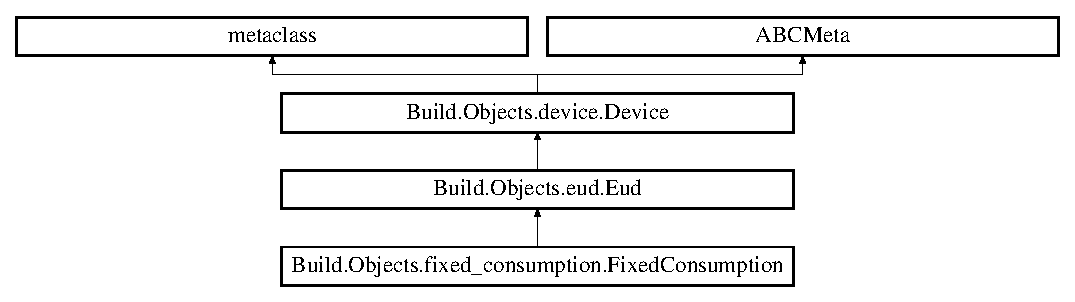
\includegraphics[height=3.612903cm]{class_build_1_1_objects_1_1fixed__consumption_1_1_fixed_consumption}
\end{center}
\end{figure}
\subsection*{Public Member Functions}
\begin{DoxyCompactItemize}
\item 
\mbox{\Hypertarget{class_build_1_1_objects_1_1fixed__consumption_1_1_fixed_consumption_ab05aa0b7096a5d0933e364496d851bbf}\label{class_build_1_1_objects_1_1fixed__consumption_1_1_fixed_consumption_ab05aa0b7096a5d0933e364496d851bbf}} 
def {\bfseries \+\_\+\+\_\+init\+\_\+\+\_\+} (self, device\+\_\+id, supervisor, total\+\_\+runtime, modulation\+\_\+interval, desired\+\_\+power\+\_\+level, schedule=None, multiday=0, time=0, msg\+\_\+latency=0)
\item 
\mbox{\Hypertarget{class_build_1_1_objects_1_1fixed__consumption_1_1_fixed_consumption_a16b7133c71492ac7e61a58d1c20676c7}\label{class_build_1_1_objects_1_1fixed__consumption_1_1_fixed_consumption_a16b7133c71492ac7e61a58d1c20676c7}} 
def \hyperlink{class_build_1_1_objects_1_1fixed__consumption_1_1_fixed_consumption_a16b7133c71492ac7e61a58d1c20676c7}{calculate\+\_\+desired\+\_\+power\+\_\+level} (self)
\begin{DoxyCompactList}\small\item\em Always returns the device\textquotesingle{}s fixed consumption levels. \end{DoxyCompactList}\item 
\mbox{\Hypertarget{class_build_1_1_objects_1_1fixed__consumption_1_1_fixed_consumption_a4738a9f17cadf91fbc76944243fbe012}\label{class_build_1_1_objects_1_1fixed__consumption_1_1_fixed_consumption_a4738a9f17cadf91fbc76944243fbe012}} 
def {\bfseries begin\+\_\+internal\+\_\+operation} (self)
\item 
\mbox{\Hypertarget{class_build_1_1_objects_1_1fixed__consumption_1_1_fixed_consumption_a16e77571984fb450ff9f2272c8b02cab}\label{class_build_1_1_objects_1_1fixed__consumption_1_1_fixed_consumption_a16e77571984fb450ff9f2272c8b02cab}} 
def {\bfseries end\+\_\+internal\+\_\+operation} (self)
\item 
\mbox{\Hypertarget{class_build_1_1_objects_1_1fixed__consumption_1_1_fixed_consumption_a61b415b965444d6f699e3e41a48df3c4}\label{class_build_1_1_objects_1_1fixed__consumption_1_1_fixed_consumption_a61b415b965444d6f699e3e41a48df3c4}} 
def {\bfseries update\+\_\+state} (self)
\item 
def \hyperlink{class_build_1_1_objects_1_1fixed__consumption_1_1_fixed_consumption_adc5b45c93ea370e11aecc8f87e2eebbc}{respond\+\_\+to\+\_\+power} (self, received\+\_\+power)
\begin{DoxyCompactList}\small\item\em If the fixed consumption does not receive all the power it would like, it simply continues to operate at the lower specified level. \end{DoxyCompactList}\item 
\mbox{\Hypertarget{class_build_1_1_objects_1_1fixed__consumption_1_1_fixed_consumption_aaba851d898ec11cbc9a960cb4461558d}\label{class_build_1_1_objects_1_1fixed__consumption_1_1_fixed_consumption_aaba851d898ec11cbc9a960cb4461558d}} 
def {\bfseries device\+\_\+specific\+\_\+calcs} (self)
\end{DoxyCompactItemize}
\subsection*{Additional Inherited Members}


\subsection{Member Function Documentation}
\mbox{\Hypertarget{class_build_1_1_objects_1_1fixed__consumption_1_1_fixed_consumption_adc5b45c93ea370e11aecc8f87e2eebbc}\label{class_build_1_1_objects_1_1fixed__consumption_1_1_fixed_consumption_adc5b45c93ea370e11aecc8f87e2eebbc}} 
\index{Build\+::\+Objects\+::fixed\+\_\+consumption\+::\+Fixed\+Consumption@{Build\+::\+Objects\+::fixed\+\_\+consumption\+::\+Fixed\+Consumption}!respond\+\_\+to\+\_\+power@{respond\+\_\+to\+\_\+power}}
\index{respond\+\_\+to\+\_\+power@{respond\+\_\+to\+\_\+power}!Build\+::\+Objects\+::fixed\+\_\+consumption\+::\+Fixed\+Consumption@{Build\+::\+Objects\+::fixed\+\_\+consumption\+::\+Fixed\+Consumption}}
\subsubsection{\texorpdfstring{respond\+\_\+to\+\_\+power()}{respond\_to\_power()}}
{\footnotesize\ttfamily def Build.\+Objects.\+fixed\+\_\+consumption.\+Fixed\+Consumption.\+respond\+\_\+to\+\_\+power (\begin{DoxyParamCaption}\item[{}]{self,  }\item[{}]{received\+\_\+power }\end{DoxyParamCaption})}



If the fixed consumption does not receive all the power it would like, it simply continues to operate at the lower specified level. 



The documentation for this class was generated from the following file\+:\begin{DoxyCompactItemize}
\item 
Build/\+Objects/fixed\+\_\+consumption.\+py\end{DoxyCompactItemize}

\hypertarget{class_build_1_1_simulation___operation_1_1logger_1_1_simulation_logger_1_1_formatter_with_header}{}\section{Build.\+Simulation\+\_\+\+Operation.\+logger.\+Simulation\+Logger.\+Formatter\+With\+Header Class Reference}
\label{class_build_1_1_simulation___operation_1_1logger_1_1_simulation_logger_1_1_formatter_with_header}\index{Build.\+Simulation\+\_\+\+Operation.\+logger.\+Simulation\+Logger.\+Formatter\+With\+Header@{Build.\+Simulation\+\_\+\+Operation.\+logger.\+Simulation\+Logger.\+Formatter\+With\+Header}}


A custom logging formatter which for the first time it is called, prepends a header to the file, before switching back to the original format style.  


Inheritance diagram for Build.\+Simulation\+\_\+\+Operation.\+logger.\+Simulation\+Logger.\+Formatter\+With\+Header\+:\begin{figure}[H]
\begin{center}
\leavevmode
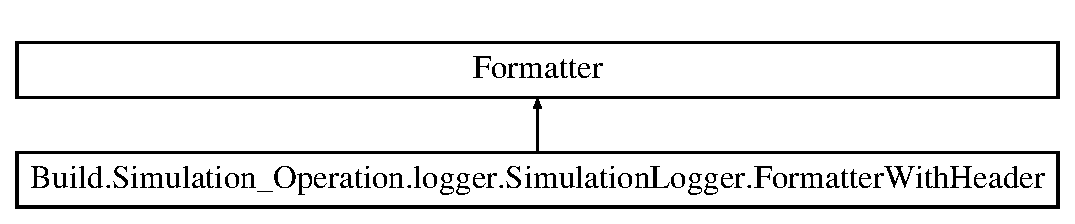
\includegraphics[height=2.000000cm]{class_build_1_1_simulation___operation_1_1logger_1_1_simulation_logger_1_1_formatter_with_header}
\end{center}
\end{figure}
\subsection*{Public Member Functions}
\begin{DoxyCompactItemize}
\item 
\mbox{\Hypertarget{class_build_1_1_simulation___operation_1_1logger_1_1_simulation_logger_1_1_formatter_with_header_a6ed2bb917fb21e709d4964039beaa105}\label{class_build_1_1_simulation___operation_1_1logger_1_1_simulation_logger_1_1_formatter_with_header_a6ed2bb917fb21e709d4964039beaa105}} 
def {\bfseries \+\_\+\+\_\+init\+\_\+\+\_\+} (self, header, fmt=None, datefmt=None, style=\textquotesingle{}\%\textquotesingle{})
\item 
\mbox{\Hypertarget{class_build_1_1_simulation___operation_1_1logger_1_1_simulation_logger_1_1_formatter_with_header_afa321e7f80452748fec676dd42ab70bc}\label{class_build_1_1_simulation___operation_1_1logger_1_1_simulation_logger_1_1_formatter_with_header_afa321e7f80452748fec676dd42ab70bc}} 
def {\bfseries first\+\_\+line\+\_\+format} (self, record)
\end{DoxyCompactItemize}
\subsection*{Public Attributes}
\begin{DoxyCompactItemize}
\item 
\mbox{\Hypertarget{class_build_1_1_simulation___operation_1_1logger_1_1_simulation_logger_1_1_formatter_with_header_a0f60bb435e92c198acb771511ed8eeee}\label{class_build_1_1_simulation___operation_1_1logger_1_1_simulation_logger_1_1_formatter_with_header_a0f60bb435e92c198acb771511ed8eeee}} 
{\bfseries header}
\item 
\mbox{\Hypertarget{class_build_1_1_simulation___operation_1_1logger_1_1_simulation_logger_1_1_formatter_with_header_a4240865ecf6ee3bad4a5e64aedcfa38b}\label{class_build_1_1_simulation___operation_1_1logger_1_1_simulation_logger_1_1_formatter_with_header_a4240865ecf6ee3bad4a5e64aedcfa38b}} 
{\bfseries format}
\end{DoxyCompactItemize}


\subsection{Detailed Description}
A custom logging formatter which for the first time it is called, prepends a header to the file, before switching back to the original format style. 



The documentation for this class was generated from the following file\+:\begin{DoxyCompactItemize}
\item 
Build/\+Simulation\+\_\+\+Operation/logger.\+py\end{DoxyCompactItemize}

\hypertarget{class_build_1_1_objects_1_1grid__controller_1_1_g_c_marginal_price_logic}{}\section{Build.\+Objects.\+grid\+\_\+controller.\+G\+C\+Marginal\+Price\+Logic Class Reference}
\label{class_build_1_1_objects_1_1grid__controller_1_1_g_c_marginal_price_logic}\index{Build.\+Objects.\+grid\+\_\+controller.\+G\+C\+Marginal\+Price\+Logic@{Build.\+Objects.\+grid\+\_\+controller.\+G\+C\+Marginal\+Price\+Logic}}
Inheritance diagram for Build.\+Objects.\+grid\+\_\+controller.\+G\+C\+Marginal\+Price\+Logic\+:\begin{figure}[H]
\begin{center}
\leavevmode
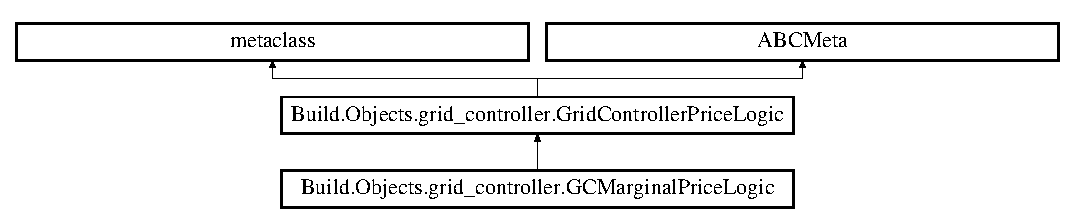
\includegraphics[height=2.568807cm]{class_build_1_1_objects_1_1grid__controller_1_1_g_c_marginal_price_logic}
\end{center}
\end{figure}
\subsection*{Public Member Functions}
\begin{DoxyCompactItemize}
\item 
def \hyperlink{class_build_1_1_objects_1_1grid__controller_1_1_g_c_marginal_price_logic_a5435c8f548b19bbc4ef6b596f49ea6ce}{\+\_\+\+\_\+init\+\_\+\+\_\+} (self, price\+\_\+history\+\_\+interval, initial\+\_\+price, price\+\_\+announce\+\_\+threshold)
\item 
def \hyperlink{class_build_1_1_objects_1_1grid__controller_1_1_g_c_marginal_price_logic_a9a5f8b1d25f916868bf8da79e12406ed}{calc\+\_\+price} (self, neighbor\+\_\+prices=None, loads=None, requested=None, allocated=None)
\begin{DoxyCompactList}\small\item\em Price is a function of the neighbors prices who have allocated to this device and utility meter prices. \end{DoxyCompactList}\end{DoxyCompactItemize}


\subsection{Constructor \& Destructor Documentation}
\mbox{\Hypertarget{class_build_1_1_objects_1_1grid__controller_1_1_g_c_marginal_price_logic_a5435c8f548b19bbc4ef6b596f49ea6ce}\label{class_build_1_1_objects_1_1grid__controller_1_1_g_c_marginal_price_logic_a5435c8f548b19bbc4ef6b596f49ea6ce}} 
\index{Build\+::\+Objects\+::grid\+\_\+controller\+::\+G\+C\+Marginal\+Price\+Logic@{Build\+::\+Objects\+::grid\+\_\+controller\+::\+G\+C\+Marginal\+Price\+Logic}!\+\_\+\+\_\+init\+\_\+\+\_\+@{\+\_\+\+\_\+init\+\_\+\+\_\+}}
\index{\+\_\+\+\_\+init\+\_\+\+\_\+@{\+\_\+\+\_\+init\+\_\+\+\_\+}!Build\+::\+Objects\+::grid\+\_\+controller\+::\+G\+C\+Marginal\+Price\+Logic@{Build\+::\+Objects\+::grid\+\_\+controller\+::\+G\+C\+Marginal\+Price\+Logic}}
\subsubsection{\texorpdfstring{\+\_\+\+\_\+init\+\_\+\+\_\+()}{\_\_init\_\_()}}
{\footnotesize\ttfamily def Build.\+Objects.\+grid\+\_\+controller.\+G\+C\+Marginal\+Price\+Logic.\+\_\+\+\_\+init\+\_\+\+\_\+ (\begin{DoxyParamCaption}\item[{}]{self,  }\item[{}]{price\+\_\+history\+\_\+interval,  }\item[{}]{initial\+\_\+price,  }\item[{}]{price\+\_\+announce\+\_\+threshold }\end{DoxyParamCaption})}


\begin{DoxyParams}{Parameters}
{\em price\+\_\+history\+\_\+interval} & the length of the interval to calculate the average price for and store in memory \\
\hline
{\em initial} & price the initial price of this grid controller \\
\hline
{\em price\+\_\+announce\+\_\+threshold} & the difference in prices before announcing your new local price to neighbors \\
\hline
\end{DoxyParams}


\subsection{Member Function Documentation}
\mbox{\Hypertarget{class_build_1_1_objects_1_1grid__controller_1_1_g_c_marginal_price_logic_a9a5f8b1d25f916868bf8da79e12406ed}\label{class_build_1_1_objects_1_1grid__controller_1_1_g_c_marginal_price_logic_a9a5f8b1d25f916868bf8da79e12406ed}} 
\index{Build\+::\+Objects\+::grid\+\_\+controller\+::\+G\+C\+Marginal\+Price\+Logic@{Build\+::\+Objects\+::grid\+\_\+controller\+::\+G\+C\+Marginal\+Price\+Logic}!calc\+\_\+price@{calc\+\_\+price}}
\index{calc\+\_\+price@{calc\+\_\+price}!Build\+::\+Objects\+::grid\+\_\+controller\+::\+G\+C\+Marginal\+Price\+Logic@{Build\+::\+Objects\+::grid\+\_\+controller\+::\+G\+C\+Marginal\+Price\+Logic}}
\subsubsection{\texorpdfstring{calc\+\_\+price()}{calc\_price()}}
{\footnotesize\ttfamily def Build.\+Objects.\+grid\+\_\+controller.\+G\+C\+Marginal\+Price\+Logic.\+calc\+\_\+price (\begin{DoxyParamCaption}\item[{}]{self,  }\item[{}]{neighbor\+\_\+prices = {\ttfamily None},  }\item[{}]{loads = {\ttfamily None},  }\item[{}]{requested = {\ttfamily None},  }\item[{}]{allocated = {\ttfamily None} }\end{DoxyParamCaption})}



Price is a function of the neighbors prices who have allocated to this device and utility meter prices. 


\begin{DoxyParams}{Parameters}
{\em neighbor\+\_\+prices} & the dictionary of connected device id\textquotesingle{}s and their prices \\
\hline
{\em loads} & dictionary of connected device id\textquotesingle{}s and current loads with those devices \\
\hline
{\em requested} & dictionary of connected device id\textquotesingle{}s and current requests to and from those devices \\
\hline
{\em allocated} & the dictionary of connected device id\textquotesingle{}s and allocated by and to those devices. \\
\hline
\end{DoxyParams}
\begin{DoxyReturn}{Returns}
the calculated price based on the input variables. 
\end{DoxyReturn}


The documentation for this class was generated from the following file\+:\begin{DoxyCompactItemize}
\item 
Build/\+Objects/grid\+\_\+controller.\+py\end{DoxyCompactItemize}

\hypertarget{class_build_1_1_objects_1_1grid__controller_1_1_g_c_marginal_price_logic_b}{}\section{Build.\+Objects.\+grid\+\_\+controller.\+G\+C\+Marginal\+Price\+LogicB Class Reference}
\label{class_build_1_1_objects_1_1grid__controller_1_1_g_c_marginal_price_logic_b}\index{Build.\+Objects.\+grid\+\_\+controller.\+G\+C\+Marginal\+Price\+LogicB@{Build.\+Objects.\+grid\+\_\+controller.\+G\+C\+Marginal\+Price\+LogicB}}
Inheritance diagram for Build.\+Objects.\+grid\+\_\+controller.\+G\+C\+Marginal\+Price\+LogicB\+:\begin{figure}[H]
\begin{center}
\leavevmode
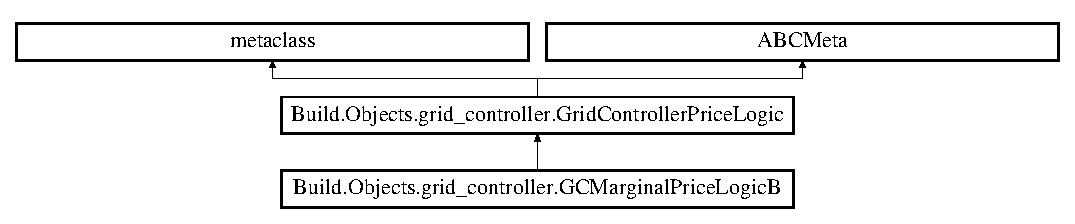
\includegraphics[height=2.568807cm]{class_build_1_1_objects_1_1grid__controller_1_1_g_c_marginal_price_logic_b}
\end{center}
\end{figure}
\subsection*{Public Member Functions}
\begin{DoxyCompactItemize}
\item 
def \hyperlink{class_build_1_1_objects_1_1grid__controller_1_1_g_c_marginal_price_logic_b_a74e1d712f6e032bd45240d28d892c368}{\+\_\+\+\_\+init\+\_\+\+\_\+} (self, price\+\_\+history\+\_\+interval, initial\+\_\+price, price\+\_\+announce\+\_\+threshold)
\item 
def \hyperlink{class_build_1_1_objects_1_1grid__controller_1_1_g_c_marginal_price_logic_b_a3f0d251ac1acb87e09895cffbbe364f2}{calc\+\_\+price} (self, neighbor\+\_\+prices=None, loads=None, requested=None, allocated=None)
\begin{DoxyCompactList}\small\item\em Price is a function of the neighbors prices who have allocated to this device and utility meter prices. \end{DoxyCompactList}\end{DoxyCompactItemize}


\subsection{Constructor \& Destructor Documentation}
\mbox{\Hypertarget{class_build_1_1_objects_1_1grid__controller_1_1_g_c_marginal_price_logic_b_a74e1d712f6e032bd45240d28d892c368}\label{class_build_1_1_objects_1_1grid__controller_1_1_g_c_marginal_price_logic_b_a74e1d712f6e032bd45240d28d892c368}} 
\index{Build\+::\+Objects\+::grid\+\_\+controller\+::\+G\+C\+Marginal\+Price\+LogicB@{Build\+::\+Objects\+::grid\+\_\+controller\+::\+G\+C\+Marginal\+Price\+LogicB}!\+\_\+\+\_\+init\+\_\+\+\_\+@{\+\_\+\+\_\+init\+\_\+\+\_\+}}
\index{\+\_\+\+\_\+init\+\_\+\+\_\+@{\+\_\+\+\_\+init\+\_\+\+\_\+}!Build\+::\+Objects\+::grid\+\_\+controller\+::\+G\+C\+Marginal\+Price\+LogicB@{Build\+::\+Objects\+::grid\+\_\+controller\+::\+G\+C\+Marginal\+Price\+LogicB}}
\subsubsection{\texorpdfstring{\+\_\+\+\_\+init\+\_\+\+\_\+()}{\_\_init\_\_()}}
{\footnotesize\ttfamily def Build.\+Objects.\+grid\+\_\+controller.\+G\+C\+Marginal\+Price\+Logic\+B.\+\_\+\+\_\+init\+\_\+\+\_\+ (\begin{DoxyParamCaption}\item[{}]{self,  }\item[{}]{price\+\_\+history\+\_\+interval,  }\item[{}]{initial\+\_\+price,  }\item[{}]{price\+\_\+announce\+\_\+threshold }\end{DoxyParamCaption})}


\begin{DoxyParams}{Parameters}
{\em price\+\_\+history\+\_\+interval} & the length of the interval to calculate the average price for and store in memory \\
\hline
{\em initial} & price the initial price of this grid controller \\
\hline
{\em price\+\_\+announce\+\_\+threshold} & the difference in prices before announcing your new local price to neighbors \\
\hline
\end{DoxyParams}


\subsection{Member Function Documentation}
\mbox{\Hypertarget{class_build_1_1_objects_1_1grid__controller_1_1_g_c_marginal_price_logic_b_a3f0d251ac1acb87e09895cffbbe364f2}\label{class_build_1_1_objects_1_1grid__controller_1_1_g_c_marginal_price_logic_b_a3f0d251ac1acb87e09895cffbbe364f2}} 
\index{Build\+::\+Objects\+::grid\+\_\+controller\+::\+G\+C\+Marginal\+Price\+LogicB@{Build\+::\+Objects\+::grid\+\_\+controller\+::\+G\+C\+Marginal\+Price\+LogicB}!calc\+\_\+price@{calc\+\_\+price}}
\index{calc\+\_\+price@{calc\+\_\+price}!Build\+::\+Objects\+::grid\+\_\+controller\+::\+G\+C\+Marginal\+Price\+LogicB@{Build\+::\+Objects\+::grid\+\_\+controller\+::\+G\+C\+Marginal\+Price\+LogicB}}
\subsubsection{\texorpdfstring{calc\+\_\+price()}{calc\_price()}}
{\footnotesize\ttfamily def Build.\+Objects.\+grid\+\_\+controller.\+G\+C\+Marginal\+Price\+Logic\+B.\+calc\+\_\+price (\begin{DoxyParamCaption}\item[{}]{self,  }\item[{}]{neighbor\+\_\+prices = {\ttfamily None},  }\item[{}]{loads = {\ttfamily None},  }\item[{}]{requested = {\ttfamily None},  }\item[{}]{allocated = {\ttfamily None} }\end{DoxyParamCaption})}



Price is a function of the neighbors prices who have allocated to this device and utility meter prices. 


\begin{DoxyParams}{Parameters}
{\em neighbor\+\_\+prices} & the dictionary of connected device id\textquotesingle{}s and their prices \\
\hline
{\em loads} & dictionary of connected device id\textquotesingle{}s and current loads with those devices \\
\hline
{\em requested} & dictionary of connected device id\textquotesingle{}s and current requests to and from those devices \\
\hline
{\em allocated} & the dictionary of connected device id\textquotesingle{}s and allocated by and to those devices. \\
\hline
\end{DoxyParams}
\begin{DoxyReturn}{Returns}
the calculated price based on the input variables. 
\end{DoxyReturn}


The documentation for this class was generated from the following file\+:\begin{DoxyCompactItemize}
\item 
Build/\+Objects/grid\+\_\+controller.\+py\end{DoxyCompactItemize}

\hypertarget{class_build_1_1_objects_1_1grid__controller_1_1_g_c_weighted_average_price_logic}{}\section{Build.\+Objects.\+grid\+\_\+controller.\+G\+C\+Weighted\+Average\+Price\+Logic Class Reference}
\label{class_build_1_1_objects_1_1grid__controller_1_1_g_c_weighted_average_price_logic}\index{Build.\+Objects.\+grid\+\_\+controller.\+G\+C\+Weighted\+Average\+Price\+Logic@{Build.\+Objects.\+grid\+\_\+controller.\+G\+C\+Weighted\+Average\+Price\+Logic}}
Inheritance diagram for Build.\+Objects.\+grid\+\_\+controller.\+G\+C\+Weighted\+Average\+Price\+Logic\+:\begin{figure}[H]
\begin{center}
\leavevmode
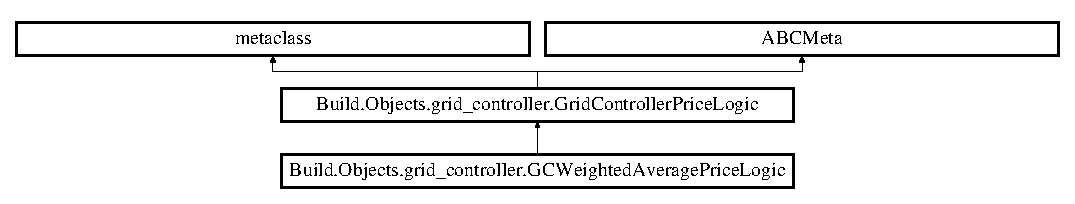
\includegraphics[height=2.295082cm]{class_build_1_1_objects_1_1grid__controller_1_1_g_c_weighted_average_price_logic}
\end{center}
\end{figure}
\subsection*{Public Member Functions}
\begin{DoxyCompactItemize}
\item 
def \hyperlink{class_build_1_1_objects_1_1grid__controller_1_1_g_c_weighted_average_price_logic_ad7ea6d4ac784744d0f2a4f0bdf6c5735}{\+\_\+\+\_\+init\+\_\+\+\_\+} (self, price\+\_\+history\+\_\+interval, initial\+\_\+price, price\+\_\+announce\+\_\+threshold)
\item 
def \hyperlink{class_build_1_1_objects_1_1grid__controller_1_1_g_c_weighted_average_price_logic_af7a4032b9379b1d65783cbe7008e5eed}{calc\+\_\+price} (self, neighbor\+\_\+prices=None, loads=None, requested=None, allocated=None)
\begin{DoxyCompactList}\small\item\em Calculates this GC\textquotesingle{}s Price as a function of the prices of its power sources, weighted by the fraction of this GC\textquotesingle{}s total power in that device is providing. \end{DoxyCompactList}\end{DoxyCompactItemize}


\subsection{Constructor \& Destructor Documentation}
\mbox{\Hypertarget{class_build_1_1_objects_1_1grid__controller_1_1_g_c_weighted_average_price_logic_ad7ea6d4ac784744d0f2a4f0bdf6c5735}\label{class_build_1_1_objects_1_1grid__controller_1_1_g_c_weighted_average_price_logic_ad7ea6d4ac784744d0f2a4f0bdf6c5735}} 
\index{Build\+::\+Objects\+::grid\+\_\+controller\+::\+G\+C\+Weighted\+Average\+Price\+Logic@{Build\+::\+Objects\+::grid\+\_\+controller\+::\+G\+C\+Weighted\+Average\+Price\+Logic}!\+\_\+\+\_\+init\+\_\+\+\_\+@{\+\_\+\+\_\+init\+\_\+\+\_\+}}
\index{\+\_\+\+\_\+init\+\_\+\+\_\+@{\+\_\+\+\_\+init\+\_\+\+\_\+}!Build\+::\+Objects\+::grid\+\_\+controller\+::\+G\+C\+Weighted\+Average\+Price\+Logic@{Build\+::\+Objects\+::grid\+\_\+controller\+::\+G\+C\+Weighted\+Average\+Price\+Logic}}
\subsubsection{\texorpdfstring{\+\_\+\+\_\+init\+\_\+\+\_\+()}{\_\_init\_\_()}}
{\footnotesize\ttfamily def Build.\+Objects.\+grid\+\_\+controller.\+G\+C\+Weighted\+Average\+Price\+Logic.\+\_\+\+\_\+init\+\_\+\+\_\+ (\begin{DoxyParamCaption}\item[{}]{self,  }\item[{}]{price\+\_\+history\+\_\+interval,  }\item[{}]{initial\+\_\+price,  }\item[{}]{price\+\_\+announce\+\_\+threshold }\end{DoxyParamCaption})}


\begin{DoxyParams}{Parameters}
{\em price\+\_\+history\+\_\+interval} & the length of the interval to calculate the average price for and store in memory \\
\hline
{\em initial} & price the initial price of this grid controller \\
\hline
{\em price\+\_\+announce\+\_\+threshold} & the difference in prices before announcing your new local price to neighbors \\
\hline
\end{DoxyParams}


\subsection{Member Function Documentation}
\mbox{\Hypertarget{class_build_1_1_objects_1_1grid__controller_1_1_g_c_weighted_average_price_logic_af7a4032b9379b1d65783cbe7008e5eed}\label{class_build_1_1_objects_1_1grid__controller_1_1_g_c_weighted_average_price_logic_af7a4032b9379b1d65783cbe7008e5eed}} 
\index{Build\+::\+Objects\+::grid\+\_\+controller\+::\+G\+C\+Weighted\+Average\+Price\+Logic@{Build\+::\+Objects\+::grid\+\_\+controller\+::\+G\+C\+Weighted\+Average\+Price\+Logic}!calc\+\_\+price@{calc\+\_\+price}}
\index{calc\+\_\+price@{calc\+\_\+price}!Build\+::\+Objects\+::grid\+\_\+controller\+::\+G\+C\+Weighted\+Average\+Price\+Logic@{Build\+::\+Objects\+::grid\+\_\+controller\+::\+G\+C\+Weighted\+Average\+Price\+Logic}}
\subsubsection{\texorpdfstring{calc\+\_\+price()}{calc\_price()}}
{\footnotesize\ttfamily def Build.\+Objects.\+grid\+\_\+controller.\+G\+C\+Weighted\+Average\+Price\+Logic.\+calc\+\_\+price (\begin{DoxyParamCaption}\item[{}]{self,  }\item[{}]{neighbor\+\_\+prices = {\ttfamily None},  }\item[{}]{loads = {\ttfamily None},  }\item[{}]{requested = {\ttfamily None},  }\item[{}]{allocated = {\ttfamily None} }\end{DoxyParamCaption})}



Calculates this GC\textquotesingle{}s Price as a function of the prices of its power sources, weighted by the fraction of this GC\textquotesingle{}s total power in that device is providing. 

If there are no current loads in, defaults to the initial price 
\begin{DoxyParams}{Parameters}
{\em neighbor\+\_\+prices} & the dictionary of connected device id\textquotesingle{}s and their prices \\
\hline
{\em loads} & dictionary of connected device id\textquotesingle{}s and current loads with those devices \\
\hline
{\em requested} & dictionary of connected device id\textquotesingle{}s and current requests to and from those devices \\
\hline
{\em allocated} & the dictionary of connected device id\textquotesingle{}s and allocated by and to those devices. \\
\hline
\end{DoxyParams}


The documentation for this class was generated from the following file\+:\begin{DoxyCompactItemize}
\item 
Build/\+Objects/grid\+\_\+controller.\+py\end{DoxyCompactItemize}

\hypertarget{class_build_1_1_objects_1_1grid__controller_1_1_grid_controller}{}\section{Build.\+Objects.\+grid\+\_\+controller.\+Grid\+Controller Class Reference}
\label{class_build_1_1_objects_1_1grid__controller_1_1_grid_controller}\index{Build.\+Objects.\+grid\+\_\+controller.\+Grid\+Controller@{Build.\+Objects.\+grid\+\_\+controller.\+Grid\+Controller}}
Inheritance diagram for Build.\+Objects.\+grid\+\_\+controller.\+Grid\+Controller\+:\begin{figure}[H]
\begin{center}
\leavevmode
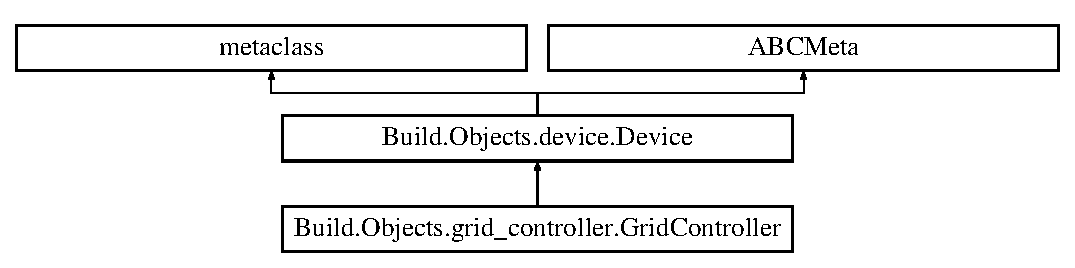
\includegraphics[height=3.000000cm]{class_build_1_1_objects_1_1grid__controller_1_1_grid_controller}
\end{center}
\end{figure}
\subsection*{Public Member Functions}
\begin{DoxyCompactItemize}
\item 
\mbox{\Hypertarget{class_build_1_1_objects_1_1grid__controller_1_1_grid_controller_a3ce9369664b081a2fbfb03252d00e3f0}\label{class_build_1_1_objects_1_1grid__controller_1_1_grid_controller_a3ce9369664b081a2fbfb03252d00e3f0}} 
def {\bfseries \+\_\+\+\_\+init\+\_\+\+\_\+} (self, device\+\_\+id, supervisor, time=0, msg\+\_\+latency=0, price\+\_\+logic=\char`\"{}\char`\"{}, price\+\_\+logic\+\_\+interval=S\+E\+C\+O\+N\+D\+S\+\_\+\+I\+N\+\_\+\+H\+O\+UR, starting\+\_\+price=0.\+1, price\+\_\+announce\+\_\+threshold=0.\+01, battery=None, min\+\_\+alloc\+\_\+response\+\_\+threshold=1.\+0, schedule=None, total\+\_\+runtime=S\+E\+C\+O\+N\+D\+S\+\_\+\+I\+N\+\_\+\+D\+AY, connected\+\_\+devices=None)
\item 
def \hyperlink{class_build_1_1_objects_1_1grid__controller_1_1_grid_controller_a9c3ee1f54a453b5008d1118d9da1b8ed}{disengage} (self)
\begin{DoxyCompactList}\small\item\em Method to be called when device is leaving the grid, and is seeking to unregister with other devices. \end{DoxyCompactList}\item 
def \hyperlink{class_build_1_1_objects_1_1grid__controller_1_1_grid_controller_a024c6220ba4e03dca547d99e1f3a39be}{turn\+\_\+on} (self, connected\+\_\+devices=None)
\begin{DoxyCompactList}\small\item\em Turns the grid controller on, registering it with all of its connected devices. \end{DoxyCompactList}\item 
def \hyperlink{class_build_1_1_objects_1_1grid__controller_1_1_grid_controller_afdea3e05f02d0c838ee8647a8f60ddf7}{turn\+\_\+off} (self)
\begin{DoxyCompactList}\small\item\em Shuts down the grid controller. \end{DoxyCompactList}\item 
def \hyperlink{class_build_1_1_objects_1_1grid__controller_1_1_grid_controller_a672af7e3a1bfe6ec323cd2d5a9e2b85a}{change\+\_\+load} (self, sender\+\_\+id, new\+\_\+load)
\begin{DoxyCompactList}\small\item\em Changes a load with a registered device. \end{DoxyCompactList}\item 
def \hyperlink{class_build_1_1_objects_1_1grid__controller_1_1_grid_controller_a5dedc78f6eca0253e0395ca38c74c4b0}{setup\+\_\+price\+\_\+calc\+\_\+schedule} (self, price\+\_\+history\+\_\+interval, total\+\_\+runtime)
\begin{DoxyCompactList}\small\item\em Recalculates the average price history at every given interval. \end{DoxyCompactList}\item 
def \hyperlink{class_build_1_1_objects_1_1grid__controller_1_1_grid_controller_a03876bc3ddc4c92dfa5e80e74978169a}{setup\+\_\+battery\+\_\+update\+\_\+schedule} (self, update\+\_\+frequency, total\+\_\+runtime)
\begin{DoxyCompactList}\small\item\em Sets up the events to recalculate the battery\textquotesingle{}s charge preference every certain period of time. \end{DoxyCompactList}\item 
def \hyperlink{class_build_1_1_objects_1_1grid__controller_1_1_grid_controller_af818cf547695cc3dbb126112cac8f453}{setup\+\_\+modulation\+\_\+schedule} (self, total\+\_\+runtime)
\begin{DoxyCompactList}\small\item\em Every 5 minutes, reevaluate this Grid Controller\textquotesingle{}s loads with modulate power and seek to optimize the distribution. \end{DoxyCompactList}\item 
def \hyperlink{class_build_1_1_objects_1_1grid__controller_1_1_grid_controller_aedf7e56f24b97d1fa1d4ff68d23cd987}{process\+\_\+register\+\_\+message} (self, sender\+\_\+id, value)
\begin{DoxyCompactList}\small\item\em Override of the device register message function. \end{DoxyCompactList}\item 
def \hyperlink{class_build_1_1_objects_1_1grid__controller_1_1_grid_controller_a7a07bb8716ac48899b8f0c1ee2e2f6fe}{process\+\_\+power\+\_\+message} (self, sender\+\_\+id, new\+\_\+power)
\begin{DoxyCompactList}\small\item\em Processes a power message, indicating power flows have changed. \end{DoxyCompactList}\item 
def \hyperlink{class_build_1_1_objects_1_1grid__controller_1_1_grid_controller_a7133aa43a9d19e42fad9c6deca385fe2}{process\+\_\+price\+\_\+message} (self, sender\+\_\+id, price, extra\+\_\+info)
\begin{DoxyCompactList}\small\item\em Processes a price message received from another device, modifying its own price based on its price logic. \end{DoxyCompactList}\item 
def \hyperlink{class_build_1_1_objects_1_1grid__controller_1_1_grid_controller_a70878c4f7a8a7cb46cc1b0097e0d91fd}{process\+\_\+request\+\_\+message} (self, sender\+\_\+id, request\+\_\+amt)
\begin{DoxyCompactList}\small\item\em Processes a request message from an E\+UD or another GC, and allocates in response whatever matches its. \end{DoxyCompactList}\item 
def \hyperlink{class_build_1_1_objects_1_1grid__controller_1_1_grid_controller_ad917e30e3b828571c02657d8052cf075}{process\+\_\+allocate\+\_\+message} (self, sender\+\_\+id, allocate\+\_\+amt)
\begin{DoxyCompactList}\small\item\em Process an allocate message from another grid controller. \end{DoxyCompactList}\item 
def \hyperlink{class_build_1_1_objects_1_1grid__controller_1_1_grid_controller_a2d1690b10f41cdef2d74895c2a971b58}{send\+\_\+power\+\_\+message} (self, target\+\_\+id, power\+\_\+amt)
\begin{DoxyCompactList}\small\item\em Sends a power message to another device. \end{DoxyCompactList}\item 
\mbox{\Hypertarget{class_build_1_1_objects_1_1grid__controller_1_1_grid_controller_ac6aa57134d55af7248149fdf9a661ffd}\label{class_build_1_1_objects_1_1grid__controller_1_1_grid_controller_ac6aa57134d55af7248149fdf9a661ffd}} 
def {\bfseries send\+\_\+price\+\_\+message} (self, target\+\_\+id, price)
\item 
def \hyperlink{class_build_1_1_objects_1_1grid__controller_1_1_grid_controller_a0eb0f617f66e5dc0c1f2f4d853251c3c}{send\+\_\+request\+\_\+message} (self, target\+\_\+id, request\+\_\+amt)
\begin{DoxyCompactList}\small\item\em Requests to receive a given amount of power from another device. \end{DoxyCompactList}\item 
def \hyperlink{class_build_1_1_objects_1_1grid__controller_1_1_grid_controller_a5ff206d2afccf703eef39dafadce5124}{send\+\_\+allocate\+\_\+message} (self, target\+\_\+id, allocate\+\_\+amt)
\begin{DoxyCompactList}\small\item\em Allocates a given quantity of power to be provided to another device. \end{DoxyCompactList}\item 
\mbox{\Hypertarget{class_build_1_1_objects_1_1grid__controller_1_1_grid_controller_aada18b526f6576563d549b9efee182df}\label{class_build_1_1_objects_1_1grid__controller_1_1_grid_controller_aada18b526f6576563d549b9efee182df}} 
def {\bfseries broadcast\+\_\+new\+\_\+price} (self, new\+\_\+price)
\item 
def \hyperlink{class_build_1_1_objects_1_1grid__controller_1_1_grid_controller_aa6a44013053b81ae9996aa21a44fac1d}{update\+\_\+battery} (self)
\begin{DoxyCompactList}\small\item\em Update the current state of the battery. \end{DoxyCompactList}\item 
def \hyperlink{class_build_1_1_objects_1_1grid__controller_1_1_grid_controller_a51734204cdfcff80c9ba18eacec07dde}{update\+\_\+average\+\_\+price\+\_\+calcs} (self)
\begin{DoxyCompactList}\small\item\em Call this function every hour during the running of the simulation. \end{DoxyCompactList}\item 
def \hyperlink{class_build_1_1_objects_1_1grid__controller_1_1_grid_controller_a59529d68b87e1814512a8c03d908d797}{recalculate\+\_\+price} (self)
\begin{DoxyCompactList}\small\item\em Recalculates the price with the Grid Controller\textquotesingle{}s price logic, and then sets the current price value. \end{DoxyCompactList}\item 
def \hyperlink{class_build_1_1_objects_1_1grid__controller_1_1_grid_controller_a8613a7012fcafee53dafc0abe1d71919}{modulate\+\_\+price} (self)
\begin{DoxyCompactList}\small\item\em Calculate this after a device has received a price message. \end{DoxyCompactList}\item 
def \hyperlink{class_build_1_1_objects_1_1grid__controller_1_1_grid_controller_aa099c2aaa311e87adde7bc663efc0779}{balance\+\_\+power} (self, source\+\_\+id, prev\+\_\+source\+\_\+power, source\+\_\+demanded\+\_\+power)
\begin{DoxyCompactList}\small\item\em Instantaneous supply-\/demand balance function, so that the net load at any given time remains at zero. \end{DoxyCompactList}\item 
def \hyperlink{class_build_1_1_objects_1_1grid__controller_1_1_grid_controller_a739bdc06f47603df13fa105dfcfaea10}{get\+\_\+allocate\+\_\+assets} (self)
\begin{DoxyCompactList}\small\item\em Sees what the GC has freely available to increase from its existing allocates compared to existing loads. \end{DoxyCompactList}\item 
def \hyperlink{class_build_1_1_objects_1_1grid__controller_1_1_grid_controller_ad984f42fc7530884d3c95fd1d4e5067e}{get\+\_\+allocate\+\_\+liabilities} (self)
\begin{DoxyCompactList}\small\item\em Sees what the GC is liable to provide other devices because of its allocation to other devices that are not being fully utilized in current loads. \end{DoxyCompactList}\item 
def \hyperlink{class_build_1_1_objects_1_1grid__controller_1_1_grid_controller_ad0475d0ecec8bd9541c940fb5e779dd1}{request\+\_\+response} (self, request\+\_\+amt)
\begin{DoxyCompactList}\small\item\em Determines how much this GC responds to a power request. \end{DoxyCompactList}\item 
\mbox{\Hypertarget{class_build_1_1_objects_1_1grid__controller_1_1_grid_controller_a41968b1bd392919861dbc0de7f153f2f}\label{class_build_1_1_objects_1_1grid__controller_1_1_grid_controller_a41968b1bd392919861dbc0de7f153f2f}} 
def \hyperlink{class_build_1_1_objects_1_1grid__controller_1_1_grid_controller_a41968b1bd392919861dbc0de7f153f2f}{modulate\+\_\+power} (self)
\begin{DoxyCompactList}\small\item\em This function determines how the Grid Controller tries to optimize its loads to satisfy its battery preference Called upon significant event changes and at regular intervals to help the GC balance its powerflows. \end{DoxyCompactList}\item 
def \hyperlink{class_build_1_1_objects_1_1grid__controller_1_1_grid_controller_ade27791e0e81bcb55583e7e711b9b5d0}{seek\+\_\+to\+\_\+obtain\+\_\+power} (self, power\+\_\+to\+\_\+obtain)
\begin{DoxyCompactList}\small\item\em Grid controller is seeking to obtain the remaining amount of power for itself to consume. \end{DoxyCompactList}\item 
def \hyperlink{class_build_1_1_objects_1_1grid__controller_1_1_grid_controller_ad85f2d1459669fe5be0d3c046c23a54b}{seek\+\_\+to\+\_\+distribute\+\_\+power} (self, power\+\_\+to\+\_\+distribute)
\begin{DoxyCompactList}\small\item\em The grid controller is seeking to distribute some quantity of power to its connected devices. \end{DoxyCompactList}\item 
def \hyperlink{class_build_1_1_objects_1_1grid__controller_1_1_grid_controller_ae5087a1b8b5278e6340b027a860353dd}{device\+\_\+specific\+\_\+calcs} (self)
\begin{DoxyCompactList}\small\item\em The grid controller is also responsible for writing its batteries calculations. \end{DoxyCompactList}\end{DoxyCompactItemize}
\subsection*{Static Public Attributes}
\begin{DoxyCompactItemize}
\item 
\mbox{\Hypertarget{class_build_1_1_objects_1_1grid__controller_1_1_grid_controller_af614a04e6d4ec6c8724676c541621095}\label{class_build_1_1_objects_1_1grid__controller_1_1_grid_controller_af614a04e6d4ec6c8724676c541621095}} 
int {\bfseries T\+R\+I\+C\+K\+L\+E\+\_\+\+P\+O\+W\+ER} = 2
\end{DoxyCompactItemize}


\subsection{Member Function Documentation}
\mbox{\Hypertarget{class_build_1_1_objects_1_1grid__controller_1_1_grid_controller_aa099c2aaa311e87adde7bc663efc0779}\label{class_build_1_1_objects_1_1grid__controller_1_1_grid_controller_aa099c2aaa311e87adde7bc663efc0779}} 
\index{Build\+::\+Objects\+::grid\+\_\+controller\+::\+Grid\+Controller@{Build\+::\+Objects\+::grid\+\_\+controller\+::\+Grid\+Controller}!balance\+\_\+power@{balance\+\_\+power}}
\index{balance\+\_\+power@{balance\+\_\+power}!Build\+::\+Objects\+::grid\+\_\+controller\+::\+Grid\+Controller@{Build\+::\+Objects\+::grid\+\_\+controller\+::\+Grid\+Controller}}
\subsubsection{\texorpdfstring{balance\+\_\+power()}{balance\_power()}}
{\footnotesize\ttfamily def Build.\+Objects.\+grid\+\_\+controller.\+Grid\+Controller.\+balance\+\_\+power (\begin{DoxyParamCaption}\item[{}]{self,  }\item[{}]{source\+\_\+id,  }\item[{}]{prev\+\_\+source\+\_\+power,  }\item[{}]{source\+\_\+demanded\+\_\+power }\end{DoxyParamCaption})}



Instantaneous supply-\/demand balance function, so that the net load at any given time remains at zero. 

To be called after this GC receives a power message, indicating external power flows have changed. The GC may not provide the entire requested amount of power if it is not able. See docs for an in-\/depth description of reasoning of this algorithm.


\begin{DoxyParams}{Parameters}
{\em source\+\_\+id} & the sender of the new amount of power. \\
\hline
{\em prev\+\_\+source\+\_\+power} & previous amount of a power flow from this GC\textquotesingle{}s perspective \\
\hline
{\em source\+\_\+demanded\+\_\+power} & the new amount of the power flow from this GC\textquotesingle{}s perspective. \\
\hline
\end{DoxyParams}
\mbox{\Hypertarget{class_build_1_1_objects_1_1grid__controller_1_1_grid_controller_a672af7e3a1bfe6ec323cd2d5a9e2b85a}\label{class_build_1_1_objects_1_1grid__controller_1_1_grid_controller_a672af7e3a1bfe6ec323cd2d5a9e2b85a}} 
\index{Build\+::\+Objects\+::grid\+\_\+controller\+::\+Grid\+Controller@{Build\+::\+Objects\+::grid\+\_\+controller\+::\+Grid\+Controller}!change\+\_\+load@{change\+\_\+load}}
\index{change\+\_\+load@{change\+\_\+load}!Build\+::\+Objects\+::grid\+\_\+controller\+::\+Grid\+Controller@{Build\+::\+Objects\+::grid\+\_\+controller\+::\+Grid\+Controller}}
\subsubsection{\texorpdfstring{change\+\_\+load()}{change\_load()}}
{\footnotesize\ttfamily def Build.\+Objects.\+grid\+\_\+controller.\+Grid\+Controller.\+change\+\_\+load (\begin{DoxyParamCaption}\item[{}]{self,  }\item[{}]{sender\+\_\+id,  }\item[{}]{new\+\_\+load }\end{DoxyParamCaption})}



Changes a load with a registered device. 

Call this before sending a power message so as to calculate the load you can actually handle considering capacities. 
\begin{DoxyParams}{Parameters}
{\em sender\+\_\+id} & the device to associate the load with \\
\hline
{\em new\+\_\+load} & the value of the new load T\+O\+DO\+: Add a maximum channel capacity for this load. \\
\hline
\end{DoxyParams}
\begin{DoxyReturn}{Returns}
the amount added to the load 
\end{DoxyReturn}
\mbox{\Hypertarget{class_build_1_1_objects_1_1grid__controller_1_1_grid_controller_ae5087a1b8b5278e6340b027a860353dd}\label{class_build_1_1_objects_1_1grid__controller_1_1_grid_controller_ae5087a1b8b5278e6340b027a860353dd}} 
\index{Build\+::\+Objects\+::grid\+\_\+controller\+::\+Grid\+Controller@{Build\+::\+Objects\+::grid\+\_\+controller\+::\+Grid\+Controller}!device\+\_\+specific\+\_\+calcs@{device\+\_\+specific\+\_\+calcs}}
\index{device\+\_\+specific\+\_\+calcs@{device\+\_\+specific\+\_\+calcs}!Build\+::\+Objects\+::grid\+\_\+controller\+::\+Grid\+Controller@{Build\+::\+Objects\+::grid\+\_\+controller\+::\+Grid\+Controller}}
\subsubsection{\texorpdfstring{device\+\_\+specific\+\_\+calcs()}{device\_specific\_calcs()}}
{\footnotesize\ttfamily def Build.\+Objects.\+grid\+\_\+controller.\+Grid\+Controller.\+device\+\_\+specific\+\_\+calcs (\begin{DoxyParamCaption}\item[{}]{self }\end{DoxyParamCaption})}



The grid controller is also responsible for writing its batteries calculations. 

Additionally, the grid controller checks the accuracy of its calculations by making sure the the difference in battery charge levels fully covers the difference in the power in and power out levels. \mbox{\Hypertarget{class_build_1_1_objects_1_1grid__controller_1_1_grid_controller_a9c3ee1f54a453b5008d1118d9da1b8ed}\label{class_build_1_1_objects_1_1grid__controller_1_1_grid_controller_a9c3ee1f54a453b5008d1118d9da1b8ed}} 
\index{Build\+::\+Objects\+::grid\+\_\+controller\+::\+Grid\+Controller@{Build\+::\+Objects\+::grid\+\_\+controller\+::\+Grid\+Controller}!disengage@{disengage}}
\index{disengage@{disengage}!Build\+::\+Objects\+::grid\+\_\+controller\+::\+Grid\+Controller@{Build\+::\+Objects\+::grid\+\_\+controller\+::\+Grid\+Controller}}
\subsubsection{\texorpdfstring{disengage()}{disengage()}}
{\footnotesize\ttfamily def Build.\+Objects.\+grid\+\_\+controller.\+Grid\+Controller.\+disengage (\begin{DoxyParamCaption}\item[{}]{self }\end{DoxyParamCaption})}



Method to be called when device is leaving the grid, and is seeking to unregister with other devices. 

Clears all other devices\textquotesingle{} records for this device before requesting to unregister and stop receiving messages. \mbox{\Hypertarget{class_build_1_1_objects_1_1grid__controller_1_1_grid_controller_a739bdc06f47603df13fa105dfcfaea10}\label{class_build_1_1_objects_1_1grid__controller_1_1_grid_controller_a739bdc06f47603df13fa105dfcfaea10}} 
\index{Build\+::\+Objects\+::grid\+\_\+controller\+::\+Grid\+Controller@{Build\+::\+Objects\+::grid\+\_\+controller\+::\+Grid\+Controller}!get\+\_\+allocate\+\_\+assets@{get\+\_\+allocate\+\_\+assets}}
\index{get\+\_\+allocate\+\_\+assets@{get\+\_\+allocate\+\_\+assets}!Build\+::\+Objects\+::grid\+\_\+controller\+::\+Grid\+Controller@{Build\+::\+Objects\+::grid\+\_\+controller\+::\+Grid\+Controller}}
\subsubsection{\texorpdfstring{get\+\_\+allocate\+\_\+assets()}{get\_allocate\_assets()}}
{\footnotesize\ttfamily def Build.\+Objects.\+grid\+\_\+controller.\+Grid\+Controller.\+get\+\_\+allocate\+\_\+assets (\begin{DoxyParamCaption}\item[{}]{self }\end{DoxyParamCaption})}



Sees what the GC has freely available to increase from its existing allocates compared to existing loads. 

\begin{DoxyReturn}{Returns}
quantity of freely available power from existing allocates 
\end{DoxyReturn}
\mbox{\Hypertarget{class_build_1_1_objects_1_1grid__controller_1_1_grid_controller_ad984f42fc7530884d3c95fd1d4e5067e}\label{class_build_1_1_objects_1_1grid__controller_1_1_grid_controller_ad984f42fc7530884d3c95fd1d4e5067e}} 
\index{Build\+::\+Objects\+::grid\+\_\+controller\+::\+Grid\+Controller@{Build\+::\+Objects\+::grid\+\_\+controller\+::\+Grid\+Controller}!get\+\_\+allocate\+\_\+liabilities@{get\+\_\+allocate\+\_\+liabilities}}
\index{get\+\_\+allocate\+\_\+liabilities@{get\+\_\+allocate\+\_\+liabilities}!Build\+::\+Objects\+::grid\+\_\+controller\+::\+Grid\+Controller@{Build\+::\+Objects\+::grid\+\_\+controller\+::\+Grid\+Controller}}
\subsubsection{\texorpdfstring{get\+\_\+allocate\+\_\+liabilities()}{get\_allocate\_liabilities()}}
{\footnotesize\ttfamily def Build.\+Objects.\+grid\+\_\+controller.\+Grid\+Controller.\+get\+\_\+allocate\+\_\+liabilities (\begin{DoxyParamCaption}\item[{}]{self }\end{DoxyParamCaption})}



Sees what the GC is liable to provide other devices because of its allocation to other devices that are not being fully utilized in current loads. 

\begin{DoxyReturn}{Returns}
quantity of excess allocate liabilities 
\end{DoxyReturn}
\mbox{\Hypertarget{class_build_1_1_objects_1_1grid__controller_1_1_grid_controller_a8613a7012fcafee53dafc0abe1d71919}\label{class_build_1_1_objects_1_1grid__controller_1_1_grid_controller_a8613a7012fcafee53dafc0abe1d71919}} 
\index{Build\+::\+Objects\+::grid\+\_\+controller\+::\+Grid\+Controller@{Build\+::\+Objects\+::grid\+\_\+controller\+::\+Grid\+Controller}!modulate\+\_\+price@{modulate\+\_\+price}}
\index{modulate\+\_\+price@{modulate\+\_\+price}!Build\+::\+Objects\+::grid\+\_\+controller\+::\+Grid\+Controller@{Build\+::\+Objects\+::grid\+\_\+controller\+::\+Grid\+Controller}}
\subsubsection{\texorpdfstring{modulate\+\_\+price()}{modulate\_price()}}
{\footnotesize\ttfamily def Build.\+Objects.\+grid\+\_\+controller.\+Grid\+Controller.\+modulate\+\_\+price (\begin{DoxyParamCaption}\item[{}]{self }\end{DoxyParamCaption})}



Calculate this after a device has received a price message. 

Iterates through the current prices of its neighbors and finds what its local price should be. \mbox{\Hypertarget{class_build_1_1_objects_1_1grid__controller_1_1_grid_controller_ad917e30e3b828571c02657d8052cf075}\label{class_build_1_1_objects_1_1grid__controller_1_1_grid_controller_ad917e30e3b828571c02657d8052cf075}} 
\index{Build\+::\+Objects\+::grid\+\_\+controller\+::\+Grid\+Controller@{Build\+::\+Objects\+::grid\+\_\+controller\+::\+Grid\+Controller}!process\+\_\+allocate\+\_\+message@{process\+\_\+allocate\+\_\+message}}
\index{process\+\_\+allocate\+\_\+message@{process\+\_\+allocate\+\_\+message}!Build\+::\+Objects\+::grid\+\_\+controller\+::\+Grid\+Controller@{Build\+::\+Objects\+::grid\+\_\+controller\+::\+Grid\+Controller}}
\subsubsection{\texorpdfstring{process\+\_\+allocate\+\_\+message()}{process\_allocate\_message()}}
{\footnotesize\ttfamily def Build.\+Objects.\+grid\+\_\+controller.\+Grid\+Controller.\+process\+\_\+allocate\+\_\+message (\begin{DoxyParamCaption}\item[{}]{self,  }\item[{}]{sender\+\_\+id,  }\item[{}]{allocate\+\_\+amt }\end{DoxyParamCaption})}



Process an allocate message from another grid controller. 

\mbox{\Hypertarget{class_build_1_1_objects_1_1grid__controller_1_1_grid_controller_a7a07bb8716ac48899b8f0c1ee2e2f6fe}\label{class_build_1_1_objects_1_1grid__controller_1_1_grid_controller_a7a07bb8716ac48899b8f0c1ee2e2f6fe}} 
\index{Build\+::\+Objects\+::grid\+\_\+controller\+::\+Grid\+Controller@{Build\+::\+Objects\+::grid\+\_\+controller\+::\+Grid\+Controller}!process\+\_\+power\+\_\+message@{process\+\_\+power\+\_\+message}}
\index{process\+\_\+power\+\_\+message@{process\+\_\+power\+\_\+message}!Build\+::\+Objects\+::grid\+\_\+controller\+::\+Grid\+Controller@{Build\+::\+Objects\+::grid\+\_\+controller\+::\+Grid\+Controller}}
\subsubsection{\texorpdfstring{process\+\_\+power\+\_\+message()}{process\_power\_message()}}
{\footnotesize\ttfamily def Build.\+Objects.\+grid\+\_\+controller.\+Grid\+Controller.\+process\+\_\+power\+\_\+message (\begin{DoxyParamCaption}\item[{}]{self,  }\item[{}]{sender\+\_\+id,  }\item[{}]{new\+\_\+power }\end{DoxyParamCaption})}



Processes a power message, indicating power flows have changed. 

First, instantaneously responds to that power flow with balance power. Then, adjusts its price based on new power flows, and finally tries to shift its power in a more optimal way. 
\begin{DoxyParams}{Parameters}
{\em sender\+\_\+id} & the device which sent the power message \\
\hline
{\em new\+\_\+power} & the new power value from the perspective of the message sender. \\
\hline
\end{DoxyParams}
\mbox{\Hypertarget{class_build_1_1_objects_1_1grid__controller_1_1_grid_controller_a7133aa43a9d19e42fad9c6deca385fe2}\label{class_build_1_1_objects_1_1grid__controller_1_1_grid_controller_a7133aa43a9d19e42fad9c6deca385fe2}} 
\index{Build\+::\+Objects\+::grid\+\_\+controller\+::\+Grid\+Controller@{Build\+::\+Objects\+::grid\+\_\+controller\+::\+Grid\+Controller}!process\+\_\+price\+\_\+message@{process\+\_\+price\+\_\+message}}
\index{process\+\_\+price\+\_\+message@{process\+\_\+price\+\_\+message}!Build\+::\+Objects\+::grid\+\_\+controller\+::\+Grid\+Controller@{Build\+::\+Objects\+::grid\+\_\+controller\+::\+Grid\+Controller}}
\subsubsection{\texorpdfstring{process\+\_\+price\+\_\+message()}{process\_price\_message()}}
{\footnotesize\ttfamily def Build.\+Objects.\+grid\+\_\+controller.\+Grid\+Controller.\+process\+\_\+price\+\_\+message (\begin{DoxyParamCaption}\item[{}]{self,  }\item[{}]{sender\+\_\+id,  }\item[{}]{price,  }\item[{}]{extra\+\_\+info }\end{DoxyParamCaption})}



Processes a price message received from another device, modifying its own price based on its price logic. 


\begin{DoxyParams}{Parameters}
{\em sender\+\_\+id} & the sender of the message \\
\hline
{\em price} & the local price received from the message sender \\
\hline
\end{DoxyParams}
\mbox{\Hypertarget{class_build_1_1_objects_1_1grid__controller_1_1_grid_controller_aedf7e56f24b97d1fa1d4ff68d23cd987}\label{class_build_1_1_objects_1_1grid__controller_1_1_grid_controller_aedf7e56f24b97d1fa1d4ff68d23cd987}} 
\index{Build\+::\+Objects\+::grid\+\_\+controller\+::\+Grid\+Controller@{Build\+::\+Objects\+::grid\+\_\+controller\+::\+Grid\+Controller}!process\+\_\+register\+\_\+message@{process\+\_\+register\+\_\+message}}
\index{process\+\_\+register\+\_\+message@{process\+\_\+register\+\_\+message}!Build\+::\+Objects\+::grid\+\_\+controller\+::\+Grid\+Controller@{Build\+::\+Objects\+::grid\+\_\+controller\+::\+Grid\+Controller}}
\subsubsection{\texorpdfstring{process\+\_\+register\+\_\+message()}{process\_register\_message()}}
{\footnotesize\ttfamily def Build.\+Objects.\+grid\+\_\+controller.\+Grid\+Controller.\+process\+\_\+register\+\_\+message (\begin{DoxyParamCaption}\item[{}]{self,  }\item[{}]{sender\+\_\+id,  }\item[{}]{value }\end{DoxyParamCaption})}



Override of the device register message function. 

When it receives a register message, also responds with information about this GC\textquotesingle{}s price.


\begin{DoxyParams}{Parameters}
{\em sender\+\_\+id} & the sender of the message informing of registering. \\
\hline
{\em value} & positive if sender is registering negative if unregistering \\
\hline
\end{DoxyParams}
\mbox{\Hypertarget{class_build_1_1_objects_1_1grid__controller_1_1_grid_controller_a70878c4f7a8a7cb46cc1b0097e0d91fd}\label{class_build_1_1_objects_1_1grid__controller_1_1_grid_controller_a70878c4f7a8a7cb46cc1b0097e0d91fd}} 
\index{Build\+::\+Objects\+::grid\+\_\+controller\+::\+Grid\+Controller@{Build\+::\+Objects\+::grid\+\_\+controller\+::\+Grid\+Controller}!process\+\_\+request\+\_\+message@{process\+\_\+request\+\_\+message}}
\index{process\+\_\+request\+\_\+message@{process\+\_\+request\+\_\+message}!Build\+::\+Objects\+::grid\+\_\+controller\+::\+Grid\+Controller@{Build\+::\+Objects\+::grid\+\_\+controller\+::\+Grid\+Controller}}
\subsubsection{\texorpdfstring{process\+\_\+request\+\_\+message()}{process\_request\_message()}}
{\footnotesize\ttfamily def Build.\+Objects.\+grid\+\_\+controller.\+Grid\+Controller.\+process\+\_\+request\+\_\+message (\begin{DoxyParamCaption}\item[{}]{self,  }\item[{}]{sender\+\_\+id,  }\item[{}]{request\+\_\+amt }\end{DoxyParamCaption})}



Processes a request message from an E\+UD or another GC, and allocates in response whatever matches its. 


\begin{DoxyParams}{Parameters}
{\em sender\+\_\+id} & the sender of the request message \\
\hline
{\em request\+\_\+amt} & the quantity of power requested from perspective of message sender \\
\hline
\end{DoxyParams}
\mbox{\Hypertarget{class_build_1_1_objects_1_1grid__controller_1_1_grid_controller_a59529d68b87e1814512a8c03d908d797}\label{class_build_1_1_objects_1_1grid__controller_1_1_grid_controller_a59529d68b87e1814512a8c03d908d797}} 
\index{Build\+::\+Objects\+::grid\+\_\+controller\+::\+Grid\+Controller@{Build\+::\+Objects\+::grid\+\_\+controller\+::\+Grid\+Controller}!recalculate\+\_\+price@{recalculate\+\_\+price}}
\index{recalculate\+\_\+price@{recalculate\+\_\+price}!Build\+::\+Objects\+::grid\+\_\+controller\+::\+Grid\+Controller@{Build\+::\+Objects\+::grid\+\_\+controller\+::\+Grid\+Controller}}
\subsubsection{\texorpdfstring{recalculate\+\_\+price()}{recalculate\_price()}}
{\footnotesize\ttfamily def Build.\+Objects.\+grid\+\_\+controller.\+Grid\+Controller.\+recalculate\+\_\+price (\begin{DoxyParamCaption}\item[{}]{self }\end{DoxyParamCaption})}



Recalculates the price with the Grid Controller\textquotesingle{}s price logic, and then sets the current price value. 

\mbox{\Hypertarget{class_build_1_1_objects_1_1grid__controller_1_1_grid_controller_ad0475d0ecec8bd9541c940fb5e779dd1}\label{class_build_1_1_objects_1_1grid__controller_1_1_grid_controller_ad0475d0ecec8bd9541c940fb5e779dd1}} 
\index{Build\+::\+Objects\+::grid\+\_\+controller\+::\+Grid\+Controller@{Build\+::\+Objects\+::grid\+\_\+controller\+::\+Grid\+Controller}!request\+\_\+response@{request\+\_\+response}}
\index{request\+\_\+response@{request\+\_\+response}!Build\+::\+Objects\+::grid\+\_\+controller\+::\+Grid\+Controller@{Build\+::\+Objects\+::grid\+\_\+controller\+::\+Grid\+Controller}}
\subsubsection{\texorpdfstring{request\+\_\+response()}{request\_response()}}
{\footnotesize\ttfamily def Build.\+Objects.\+grid\+\_\+controller.\+Grid\+Controller.\+request\+\_\+response (\begin{DoxyParamCaption}\item[{}]{self,  }\item[{}]{request\+\_\+amt }\end{DoxyParamCaption})}



Determines how much this GC responds to a power request. 

See documentation for reasoning. \begin{DoxyReturn}{Returns}
how much this device will provide in respond to that request message (negative value) 
\end{DoxyReturn}
\mbox{\Hypertarget{class_build_1_1_objects_1_1grid__controller_1_1_grid_controller_ad85f2d1459669fe5be0d3c046c23a54b}\label{class_build_1_1_objects_1_1grid__controller_1_1_grid_controller_ad85f2d1459669fe5be0d3c046c23a54b}} 
\index{Build\+::\+Objects\+::grid\+\_\+controller\+::\+Grid\+Controller@{Build\+::\+Objects\+::grid\+\_\+controller\+::\+Grid\+Controller}!seek\+\_\+to\+\_\+distribute\+\_\+power@{seek\+\_\+to\+\_\+distribute\+\_\+power}}
\index{seek\+\_\+to\+\_\+distribute\+\_\+power@{seek\+\_\+to\+\_\+distribute\+\_\+power}!Build\+::\+Objects\+::grid\+\_\+controller\+::\+Grid\+Controller@{Build\+::\+Objects\+::grid\+\_\+controller\+::\+Grid\+Controller}}
\subsubsection{\texorpdfstring{seek\+\_\+to\+\_\+distribute\+\_\+power()}{seek\_to\_distribute\_power()}}
{\footnotesize\ttfamily def Build.\+Objects.\+grid\+\_\+controller.\+Grid\+Controller.\+seek\+\_\+to\+\_\+distribute\+\_\+power (\begin{DoxyParamCaption}\item[{}]{self,  }\item[{}]{power\+\_\+to\+\_\+distribute }\end{DoxyParamCaption})}



The grid controller is seeking to distribute some quantity of power to its connected devices. 

Currently, only tries to sell it off the utility meter, and whatever cannot be distributed is added back to battery.


\begin{DoxyParams}{Parameters}
{\em power\+\_\+to\+\_\+distribute} & the amount of power that this grid controller would like to distribute to other sources must be a positive value. \\
\hline
\end{DoxyParams}
\mbox{\Hypertarget{class_build_1_1_objects_1_1grid__controller_1_1_grid_controller_ade27791e0e81bcb55583e7e711b9b5d0}\label{class_build_1_1_objects_1_1grid__controller_1_1_grid_controller_ade27791e0e81bcb55583e7e711b9b5d0}} 
\index{Build\+::\+Objects\+::grid\+\_\+controller\+::\+Grid\+Controller@{Build\+::\+Objects\+::grid\+\_\+controller\+::\+Grid\+Controller}!seek\+\_\+to\+\_\+obtain\+\_\+power@{seek\+\_\+to\+\_\+obtain\+\_\+power}}
\index{seek\+\_\+to\+\_\+obtain\+\_\+power@{seek\+\_\+to\+\_\+obtain\+\_\+power}!Build\+::\+Objects\+::grid\+\_\+controller\+::\+Grid\+Controller@{Build\+::\+Objects\+::grid\+\_\+controller\+::\+Grid\+Controller}}
\subsubsection{\texorpdfstring{seek\+\_\+to\+\_\+obtain\+\_\+power()}{seek\_to\_obtain\_power()}}
{\footnotesize\ttfamily def Build.\+Objects.\+grid\+\_\+controller.\+Grid\+Controller.\+seek\+\_\+to\+\_\+obtain\+\_\+power (\begin{DoxyParamCaption}\item[{}]{self,  }\item[{}]{power\+\_\+to\+\_\+obtain }\end{DoxyParamCaption})}



Grid controller is seeking to obtain the remaining amount of power for itself to consume. 

Currently, only goes to the utility meters if it is connected and tries to shift power onto them, does not do any shifting on less expensive power sources/grid controller optimization. 
\begin{DoxyParams}{Parameters}
{\em power\+\_\+to\+\_\+obtain} & the amount of power this grid controller would like to obtain from other sources. Must be positive. \\
\hline
\end{DoxyParams}
\mbox{\Hypertarget{class_build_1_1_objects_1_1grid__controller_1_1_grid_controller_a5ff206d2afccf703eef39dafadce5124}\label{class_build_1_1_objects_1_1grid__controller_1_1_grid_controller_a5ff206d2afccf703eef39dafadce5124}} 
\index{Build\+::\+Objects\+::grid\+\_\+controller\+::\+Grid\+Controller@{Build\+::\+Objects\+::grid\+\_\+controller\+::\+Grid\+Controller}!send\+\_\+allocate\+\_\+message@{send\+\_\+allocate\+\_\+message}}
\index{send\+\_\+allocate\+\_\+message@{send\+\_\+allocate\+\_\+message}!Build\+::\+Objects\+::grid\+\_\+controller\+::\+Grid\+Controller@{Build\+::\+Objects\+::grid\+\_\+controller\+::\+Grid\+Controller}}
\subsubsection{\texorpdfstring{send\+\_\+allocate\+\_\+message()}{send\_allocate\_message()}}
{\footnotesize\ttfamily def Build.\+Objects.\+grid\+\_\+controller.\+Grid\+Controller.\+send\+\_\+allocate\+\_\+message (\begin{DoxyParamCaption}\item[{}]{self,  }\item[{}]{target\+\_\+id,  }\item[{}]{allocate\+\_\+amt }\end{DoxyParamCaption})}



Allocates a given quantity of power to be provided to another device. 

\mbox{\Hypertarget{class_build_1_1_objects_1_1grid__controller_1_1_grid_controller_a2d1690b10f41cdef2d74895c2a971b58}\label{class_build_1_1_objects_1_1grid__controller_1_1_grid_controller_a2d1690b10f41cdef2d74895c2a971b58}} 
\index{Build\+::\+Objects\+::grid\+\_\+controller\+::\+Grid\+Controller@{Build\+::\+Objects\+::grid\+\_\+controller\+::\+Grid\+Controller}!send\+\_\+power\+\_\+message@{send\+\_\+power\+\_\+message}}
\index{send\+\_\+power\+\_\+message@{send\+\_\+power\+\_\+message}!Build\+::\+Objects\+::grid\+\_\+controller\+::\+Grid\+Controller@{Build\+::\+Objects\+::grid\+\_\+controller\+::\+Grid\+Controller}}
\subsubsection{\texorpdfstring{send\+\_\+power\+\_\+message()}{send\_power\_message()}}
{\footnotesize\ttfamily def Build.\+Objects.\+grid\+\_\+controller.\+Grid\+Controller.\+send\+\_\+power\+\_\+message (\begin{DoxyParamCaption}\item[{}]{self,  }\item[{}]{target\+\_\+id,  }\item[{}]{power\+\_\+amt }\end{DoxyParamCaption})}



Sends a power message to another device. 


\begin{DoxyParams}{Parameters}
{\em target\+\_\+id} & the recipient of the power message \\
\hline
{\em power\+\_\+amt} & the quantity of the new power flow from this device\textquotesingle{}s perspective \\
\hline
\end{DoxyParams}
\mbox{\Hypertarget{class_build_1_1_objects_1_1grid__controller_1_1_grid_controller_a0eb0f617f66e5dc0c1f2f4d853251c3c}\label{class_build_1_1_objects_1_1grid__controller_1_1_grid_controller_a0eb0f617f66e5dc0c1f2f4d853251c3c}} 
\index{Build\+::\+Objects\+::grid\+\_\+controller\+::\+Grid\+Controller@{Build\+::\+Objects\+::grid\+\_\+controller\+::\+Grid\+Controller}!send\+\_\+request\+\_\+message@{send\+\_\+request\+\_\+message}}
\index{send\+\_\+request\+\_\+message@{send\+\_\+request\+\_\+message}!Build\+::\+Objects\+::grid\+\_\+controller\+::\+Grid\+Controller@{Build\+::\+Objects\+::grid\+\_\+controller\+::\+Grid\+Controller}}
\subsubsection{\texorpdfstring{send\+\_\+request\+\_\+message()}{send\_request\_message()}}
{\footnotesize\ttfamily def Build.\+Objects.\+grid\+\_\+controller.\+Grid\+Controller.\+send\+\_\+request\+\_\+message (\begin{DoxyParamCaption}\item[{}]{self,  }\item[{}]{target\+\_\+id,  }\item[{}]{request\+\_\+amt }\end{DoxyParamCaption})}



Requests to receive a given amount of power from another device. 

\mbox{\Hypertarget{class_build_1_1_objects_1_1grid__controller_1_1_grid_controller_a03876bc3ddc4c92dfa5e80e74978169a}\label{class_build_1_1_objects_1_1grid__controller_1_1_grid_controller_a03876bc3ddc4c92dfa5e80e74978169a}} 
\index{Build\+::\+Objects\+::grid\+\_\+controller\+::\+Grid\+Controller@{Build\+::\+Objects\+::grid\+\_\+controller\+::\+Grid\+Controller}!setup\+\_\+battery\+\_\+update\+\_\+schedule@{setup\+\_\+battery\+\_\+update\+\_\+schedule}}
\index{setup\+\_\+battery\+\_\+update\+\_\+schedule@{setup\+\_\+battery\+\_\+update\+\_\+schedule}!Build\+::\+Objects\+::grid\+\_\+controller\+::\+Grid\+Controller@{Build\+::\+Objects\+::grid\+\_\+controller\+::\+Grid\+Controller}}
\subsubsection{\texorpdfstring{setup\+\_\+battery\+\_\+update\+\_\+schedule()}{setup\_battery\_update\_schedule()}}
{\footnotesize\ttfamily def Build.\+Objects.\+grid\+\_\+controller.\+Grid\+Controller.\+setup\+\_\+battery\+\_\+update\+\_\+schedule (\begin{DoxyParamCaption}\item[{}]{self,  }\item[{}]{update\+\_\+frequency,  }\item[{}]{total\+\_\+runtime }\end{DoxyParamCaption})}



Sets up the events to recalculate the battery\textquotesingle{}s charge preference every certain period of time. 


\begin{DoxyParams}{Parameters}
{\em update\+\_\+frequency} & how frequently prices should be recalculated. \\
\hline
{\em total\+\_\+runtime} & the total runtime of the simulation, this will setup events up until that time \\
\hline
\end{DoxyParams}
\mbox{\Hypertarget{class_build_1_1_objects_1_1grid__controller_1_1_grid_controller_af818cf547695cc3dbb126112cac8f453}\label{class_build_1_1_objects_1_1grid__controller_1_1_grid_controller_af818cf547695cc3dbb126112cac8f453}} 
\index{Build\+::\+Objects\+::grid\+\_\+controller\+::\+Grid\+Controller@{Build\+::\+Objects\+::grid\+\_\+controller\+::\+Grid\+Controller}!setup\+\_\+modulation\+\_\+schedule@{setup\+\_\+modulation\+\_\+schedule}}
\index{setup\+\_\+modulation\+\_\+schedule@{setup\+\_\+modulation\+\_\+schedule}!Build\+::\+Objects\+::grid\+\_\+controller\+::\+Grid\+Controller@{Build\+::\+Objects\+::grid\+\_\+controller\+::\+Grid\+Controller}}
\subsubsection{\texorpdfstring{setup\+\_\+modulation\+\_\+schedule()}{setup\_modulation\_schedule()}}
{\footnotesize\ttfamily def Build.\+Objects.\+grid\+\_\+controller.\+Grid\+Controller.\+setup\+\_\+modulation\+\_\+schedule (\begin{DoxyParamCaption}\item[{}]{self,  }\item[{}]{total\+\_\+runtime }\end{DoxyParamCaption})}



Every 5 minutes, reevaluate this Grid Controller\textquotesingle{}s loads with modulate power and seek to optimize the distribution. 


\begin{DoxyParams}{Parameters}
{\em total\+\_\+runtime} & the length of the simulation in seconds. \\
\hline
\end{DoxyParams}
\mbox{\Hypertarget{class_build_1_1_objects_1_1grid__controller_1_1_grid_controller_a5dedc78f6eca0253e0395ca38c74c4b0}\label{class_build_1_1_objects_1_1grid__controller_1_1_grid_controller_a5dedc78f6eca0253e0395ca38c74c4b0}} 
\index{Build\+::\+Objects\+::grid\+\_\+controller\+::\+Grid\+Controller@{Build\+::\+Objects\+::grid\+\_\+controller\+::\+Grid\+Controller}!setup\+\_\+price\+\_\+calc\+\_\+schedule@{setup\+\_\+price\+\_\+calc\+\_\+schedule}}
\index{setup\+\_\+price\+\_\+calc\+\_\+schedule@{setup\+\_\+price\+\_\+calc\+\_\+schedule}!Build\+::\+Objects\+::grid\+\_\+controller\+::\+Grid\+Controller@{Build\+::\+Objects\+::grid\+\_\+controller\+::\+Grid\+Controller}}
\subsubsection{\texorpdfstring{setup\+\_\+price\+\_\+calc\+\_\+schedule()}{setup\_price\_calc\_schedule()}}
{\footnotesize\ttfamily def Build.\+Objects.\+grid\+\_\+controller.\+Grid\+Controller.\+setup\+\_\+price\+\_\+calc\+\_\+schedule (\begin{DoxyParamCaption}\item[{}]{self,  }\item[{}]{price\+\_\+history\+\_\+interval,  }\item[{}]{total\+\_\+runtime }\end{DoxyParamCaption})}



Recalculates the average price history at every given interval. 


\begin{DoxyParams}[1]{Parameters}
\mbox{\tt in}  & {\em price\+\_\+history\+\_\+interval} & how frequently prices should be recalculated. \\
\hline
\mbox{\tt in}  & {\em total\+\_\+runtime} & the total runtime of the simulation, this will setup events up until that time \\
\hline
\end{DoxyParams}
\mbox{\Hypertarget{class_build_1_1_objects_1_1grid__controller_1_1_grid_controller_afdea3e05f02d0c838ee8647a8f60ddf7}\label{class_build_1_1_objects_1_1grid__controller_1_1_grid_controller_afdea3e05f02d0c838ee8647a8f60ddf7}} 
\index{Build\+::\+Objects\+::grid\+\_\+controller\+::\+Grid\+Controller@{Build\+::\+Objects\+::grid\+\_\+controller\+::\+Grid\+Controller}!turn\+\_\+off@{turn\+\_\+off}}
\index{turn\+\_\+off@{turn\+\_\+off}!Build\+::\+Objects\+::grid\+\_\+controller\+::\+Grid\+Controller@{Build\+::\+Objects\+::grid\+\_\+controller\+::\+Grid\+Controller}}
\subsubsection{\texorpdfstring{turn\+\_\+off()}{turn\_off()}}
{\footnotesize\ttfamily def Build.\+Objects.\+grid\+\_\+controller.\+Grid\+Controller.\+turn\+\_\+off (\begin{DoxyParamCaption}\item[{}]{self }\end{DoxyParamCaption})}



Shuts down the grid controller. 

Stop power flows. Send messages to all connected devices to reset their negotiations with this grid controller to zero. \mbox{\Hypertarget{class_build_1_1_objects_1_1grid__controller_1_1_grid_controller_a024c6220ba4e03dca547d99e1f3a39be}\label{class_build_1_1_objects_1_1grid__controller_1_1_grid_controller_a024c6220ba4e03dca547d99e1f3a39be}} 
\index{Build\+::\+Objects\+::grid\+\_\+controller\+::\+Grid\+Controller@{Build\+::\+Objects\+::grid\+\_\+controller\+::\+Grid\+Controller}!turn\+\_\+on@{turn\+\_\+on}}
\index{turn\+\_\+on@{turn\+\_\+on}!Build\+::\+Objects\+::grid\+\_\+controller\+::\+Grid\+Controller@{Build\+::\+Objects\+::grid\+\_\+controller\+::\+Grid\+Controller}}
\subsubsection{\texorpdfstring{turn\+\_\+on()}{turn\_on()}}
{\footnotesize\ttfamily def Build.\+Objects.\+grid\+\_\+controller.\+Grid\+Controller.\+turn\+\_\+on (\begin{DoxyParamCaption}\item[{}]{self,  }\item[{}]{connected\+\_\+devices = {\ttfamily None} }\end{DoxyParamCaption})}



Turns the grid controller on, registering it with all of its connected devices. 


\begin{DoxyParams}{Parameters}
{\em connected\+\_\+devices} & the devices that this GC is connected to (default to already connected devices) \\
\hline
\end{DoxyParams}
\mbox{\Hypertarget{class_build_1_1_objects_1_1grid__controller_1_1_grid_controller_a51734204cdfcff80c9ba18eacec07dde}\label{class_build_1_1_objects_1_1grid__controller_1_1_grid_controller_a51734204cdfcff80c9ba18eacec07dde}} 
\index{Build\+::\+Objects\+::grid\+\_\+controller\+::\+Grid\+Controller@{Build\+::\+Objects\+::grid\+\_\+controller\+::\+Grid\+Controller}!update\+\_\+average\+\_\+price\+\_\+calcs@{update\+\_\+average\+\_\+price\+\_\+calcs}}
\index{update\+\_\+average\+\_\+price\+\_\+calcs@{update\+\_\+average\+\_\+price\+\_\+calcs}!Build\+::\+Objects\+::grid\+\_\+controller\+::\+Grid\+Controller@{Build\+::\+Objects\+::grid\+\_\+controller\+::\+Grid\+Controller}}
\subsubsection{\texorpdfstring{update\+\_\+average\+\_\+price\+\_\+calcs()}{update\_average\_price\_calcs()}}
{\footnotesize\ttfamily def Build.\+Objects.\+grid\+\_\+controller.\+Grid\+Controller.\+update\+\_\+average\+\_\+price\+\_\+calcs (\begin{DoxyParamCaption}\item[{}]{self }\end{DoxyParamCaption})}



Call this function every hour during the running of the simulation. 

This will reevaluate the current running hourly price and total average price statistics so that it can base its current price based on those. \mbox{\Hypertarget{class_build_1_1_objects_1_1grid__controller_1_1_grid_controller_aa6a44013053b81ae9996aa21a44fac1d}\label{class_build_1_1_objects_1_1grid__controller_1_1_grid_controller_aa6a44013053b81ae9996aa21a44fac1d}} 
\index{Build\+::\+Objects\+::grid\+\_\+controller\+::\+Grid\+Controller@{Build\+::\+Objects\+::grid\+\_\+controller\+::\+Grid\+Controller}!update\+\_\+battery@{update\+\_\+battery}}
\index{update\+\_\+battery@{update\+\_\+battery}!Build\+::\+Objects\+::grid\+\_\+controller\+::\+Grid\+Controller@{Build\+::\+Objects\+::grid\+\_\+controller\+::\+Grid\+Controller}}
\subsubsection{\texorpdfstring{update\+\_\+battery()}{update\_battery()}}
{\footnotesize\ttfamily def Build.\+Objects.\+grid\+\_\+controller.\+Grid\+Controller.\+update\+\_\+battery (\begin{DoxyParamCaption}\item[{}]{self }\end{DoxyParamCaption})}



Update the current state of the battery. 

Call this function every five minutes or on price change. Informs the battery of its average prices and hourly prices so that the battery can determine its charge preference accordingly, and recalculate its current state of charge 

The documentation for this class was generated from the following file\+:\begin{DoxyCompactItemize}
\item 
Build/\+Objects/grid\+\_\+controller.\+py\end{DoxyCompactItemize}

\hypertarget{class_build_1_1_objects_1_1grid__controller_1_1_grid_controller_price_logic}{}\section{Build.\+Objects.\+grid\+\_\+controller.\+Grid\+Controller\+Price\+Logic Class Reference}
\label{class_build_1_1_objects_1_1grid__controller_1_1_grid_controller_price_logic}\index{Build.\+Objects.\+grid\+\_\+controller.\+Grid\+Controller\+Price\+Logic@{Build.\+Objects.\+grid\+\_\+controller.\+Grid\+Controller\+Price\+Logic}}


The abstract class for all grid controller price logics.  


Inheritance diagram for Build.\+Objects.\+grid\+\_\+controller.\+Grid\+Controller\+Price\+Logic\+:\begin{figure}[H]
\begin{center}
\leavevmode
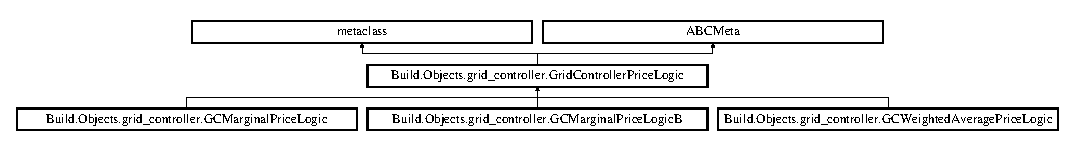
\includegraphics[height=1.530055cm]{class_build_1_1_objects_1_1grid__controller_1_1_grid_controller_price_logic}
\end{center}
\end{figure}
\subsection*{Public Member Functions}
\begin{DoxyCompactItemize}
\item 
def \hyperlink{class_build_1_1_objects_1_1grid__controller_1_1_grid_controller_price_logic_ad41a0d1f0d453c278938a1615352a2a3}{\+\_\+\+\_\+init\+\_\+\+\_\+} (self, price\+\_\+history\+\_\+interval, initial\+\_\+price, price\+\_\+announce\+\_\+threshold)
\item 
\mbox{\Hypertarget{class_build_1_1_objects_1_1grid__controller_1_1_grid_controller_price_logic_afa3d44f846108a1c8be4818b50347597}\label{class_build_1_1_objects_1_1grid__controller_1_1_grid_controller_price_logic_afa3d44f846108a1c8be4818b50347597}} 
def \hyperlink{class_build_1_1_objects_1_1grid__controller_1_1_grid_controller_price_logic_afa3d44f846108a1c8be4818b50347597}{get\+\_\+initial\+\_\+price} (self)
\begin{DoxyCompactList}\small\item\em Returns the devices initial price level. \end{DoxyCompactList}\item 
def \hyperlink{class_build_1_1_objects_1_1grid__controller_1_1_grid_controller_price_logic_a311d9e78fc37960b0404f60259ac92f3}{get\+\_\+price\+\_\+announce\+\_\+threshold} (self)
\begin{DoxyCompactList}\small\item\em A method to determine the minimum price difference which should cause the grid controller to broadcast its new price to a specified subset of its connected devices. \end{DoxyCompactList}\item 
\mbox{\Hypertarget{class_build_1_1_objects_1_1grid__controller_1_1_grid_controller_price_logic_abfafee704233af88153846874f1c7d98}\label{class_build_1_1_objects_1_1grid__controller_1_1_grid_controller_price_logic_abfafee704233af88153846874f1c7d98}} 
def \hyperlink{class_build_1_1_objects_1_1grid__controller_1_1_grid_controller_price_logic_abfafee704233af88153846874f1c7d98}{get\+\_\+forecast\+\_\+price} (self, time)
\begin{DoxyCompactList}\small\item\em Gets the predicted price of this grid controller at the specified time (in seconds) \end{DoxyCompactList}\item 
\mbox{\Hypertarget{class_build_1_1_objects_1_1grid__controller_1_1_grid_controller_price_logic_a58470569ce8fe9ce1907e3f8784426a5}\label{class_build_1_1_objects_1_1grid__controller_1_1_grid_controller_price_logic_a58470569ce8fe9ce1907e3f8784426a5}} 
def \hyperlink{class_build_1_1_objects_1_1grid__controller_1_1_grid_controller_price_logic_a58470569ce8fe9ce1907e3f8784426a5}{get\+\_\+price\+\_\+history\+\_\+interval} (self)
\begin{DoxyCompactList}\small\item\em Gets the length of a price intervals. \end{DoxyCompactList}\item 
def \hyperlink{class_build_1_1_objects_1_1grid__controller_1_1_grid_controller_price_logic_a9c0d6f8e499488e3ae75ad3779876cfd}{update\+\_\+interval\+\_\+prices} (self, time)
\begin{DoxyCompactList}\small\item\em Given the current time of the device, uses the current price to set the interval prices of the GC accordingly. \end{DoxyCompactList}\item 
def \hyperlink{class_build_1_1_objects_1_1grid__controller_1_1_grid_controller_price_logic_a241ac9f19af131870e9bad6dd2b3cbc3}{update\+\_\+average\+\_\+price} (self, time)
\begin{DoxyCompactList}\small\item\em Updates the average time of the grid controller. \end{DoxyCompactList}\item 
def \hyperlink{class_build_1_1_objects_1_1grid__controller_1_1_grid_controller_price_logic_a4448f422b18640d1d00b1b43cc73d149}{get\+\_\+interval\+\_\+prices} (self)
\begin{DoxyCompactList}\small\item\em Returns the interval prices of this grid controller. \end{DoxyCompactList}\item 
def \hyperlink{class_build_1_1_objects_1_1grid__controller_1_1_grid_controller_price_logic_a83a87f838ab54ca0dbd4cb3924994c7b}{set\+\_\+current\+\_\+price} (self, price)
\begin{DoxyCompactList}\small\item\em Sets the current price to use in the price logic for calculations. \end{DoxyCompactList}\item 
def \hyperlink{class_build_1_1_objects_1_1grid__controller_1_1_grid_controller_price_logic_a8772b6c6be3c37e2249c257f8ac5e82a}{update\+\_\+prices} (self, time)
\begin{DoxyCompactList}\small\item\em Updates the interval and average price calculations stored in this price logic for this GC. \end{DoxyCompactList}\item 
def \hyperlink{class_build_1_1_objects_1_1grid__controller_1_1_grid_controller_price_logic_a2efaa2e5ead1f5d0d7d3d006940bfeba}{get\+\_\+average\+\_\+price} (self)
\item 
def \hyperlink{class_build_1_1_objects_1_1grid__controller_1_1_grid_controller_price_logic_ae4599f832b461c8fdbb66d90b95dd115}{calc\+\_\+price} (self, neighbor\+\_\+prices=None, loads=None, requested=None, allocated=None)
\begin{DoxyCompactList}\small\item\em Calculates what this current GC\textquotesingle{}s price is based on some combination of the price of its neighbors, the current request and allocated amounts. \end{DoxyCompactList}\end{DoxyCompactItemize}


\subsection{Detailed Description}
The abstract class for all grid controller price logics. 

All abstract methods must be implemented by all price logics. 

\subsection{Constructor \& Destructor Documentation}
\mbox{\Hypertarget{class_build_1_1_objects_1_1grid__controller_1_1_grid_controller_price_logic_ad41a0d1f0d453c278938a1615352a2a3}\label{class_build_1_1_objects_1_1grid__controller_1_1_grid_controller_price_logic_ad41a0d1f0d453c278938a1615352a2a3}} 
\index{Build\+::\+Objects\+::grid\+\_\+controller\+::\+Grid\+Controller\+Price\+Logic@{Build\+::\+Objects\+::grid\+\_\+controller\+::\+Grid\+Controller\+Price\+Logic}!\+\_\+\+\_\+init\+\_\+\+\_\+@{\+\_\+\+\_\+init\+\_\+\+\_\+}}
\index{\+\_\+\+\_\+init\+\_\+\+\_\+@{\+\_\+\+\_\+init\+\_\+\+\_\+}!Build\+::\+Objects\+::grid\+\_\+controller\+::\+Grid\+Controller\+Price\+Logic@{Build\+::\+Objects\+::grid\+\_\+controller\+::\+Grid\+Controller\+Price\+Logic}}
\subsubsection{\texorpdfstring{\+\_\+\+\_\+init\+\_\+\+\_\+()}{\_\_init\_\_()}}
{\footnotesize\ttfamily def Build.\+Objects.\+grid\+\_\+controller.\+Grid\+Controller\+Price\+Logic.\+\_\+\+\_\+init\+\_\+\+\_\+ (\begin{DoxyParamCaption}\item[{}]{self,  }\item[{}]{price\+\_\+history\+\_\+interval,  }\item[{}]{initial\+\_\+price,  }\item[{}]{price\+\_\+announce\+\_\+threshold }\end{DoxyParamCaption})}


\begin{DoxyParams}{Parameters}
{\em price\+\_\+history\+\_\+interval} & the length of the interval to calculate the average price for and store in memory (e.\+g. if 3600, then store hourly average prices). \\
\hline
{\em initial} & price the initial price of this grid controller \\
\hline
{\em price\+\_\+announce\+\_\+threshold} & the difference in prices before announcing your new local price to neighbors \\
\hline
\end{DoxyParams}


\subsection{Member Function Documentation}
\mbox{\Hypertarget{class_build_1_1_objects_1_1grid__controller_1_1_grid_controller_price_logic_ae4599f832b461c8fdbb66d90b95dd115}\label{class_build_1_1_objects_1_1grid__controller_1_1_grid_controller_price_logic_ae4599f832b461c8fdbb66d90b95dd115}} 
\index{Build\+::\+Objects\+::grid\+\_\+controller\+::\+Grid\+Controller\+Price\+Logic@{Build\+::\+Objects\+::grid\+\_\+controller\+::\+Grid\+Controller\+Price\+Logic}!calc\+\_\+price@{calc\+\_\+price}}
\index{calc\+\_\+price@{calc\+\_\+price}!Build\+::\+Objects\+::grid\+\_\+controller\+::\+Grid\+Controller\+Price\+Logic@{Build\+::\+Objects\+::grid\+\_\+controller\+::\+Grid\+Controller\+Price\+Logic}}
\subsubsection{\texorpdfstring{calc\+\_\+price()}{calc\_price()}}
{\footnotesize\ttfamily def Build.\+Objects.\+grid\+\_\+controller.\+Grid\+Controller\+Price\+Logic.\+calc\+\_\+price (\begin{DoxyParamCaption}\item[{}]{self,  }\item[{}]{neighbor\+\_\+prices = {\ttfamily None},  }\item[{}]{loads = {\ttfamily None},  }\item[{}]{requested = {\ttfamily None},  }\item[{}]{allocated = {\ttfamily None} }\end{DoxyParamCaption})}



Calculates what this current GC\textquotesingle{}s price is based on some combination of the price of its neighbors, the current request and allocated amounts. 

Varies between different implementations of price logics. 
\begin{DoxyParams}{Parameters}
{\em neighbor\+\_\+prices} & the dictionary of connected device id\textquotesingle{}s and their prices \\
\hline
{\em loads} & dictionary of connected device id\textquotesingle{}s and current loads with those devices \\
\hline
{\em requested} & dictionary of connected device id\textquotesingle{}s and current requests to and from those devices \\
\hline
{\em allocated} & the dictionary of connected device id\textquotesingle{}s and allocated by and to those devices. \\
\hline
\end{DoxyParams}
\begin{DoxyReturn}{Returns}
the calculated price based on the input variables. 
\end{DoxyReturn}
\mbox{\Hypertarget{class_build_1_1_objects_1_1grid__controller_1_1_grid_controller_price_logic_a2efaa2e5ead1f5d0d7d3d006940bfeba}\label{class_build_1_1_objects_1_1grid__controller_1_1_grid_controller_price_logic_a2efaa2e5ead1f5d0d7d3d006940bfeba}} 
\index{Build\+::\+Objects\+::grid\+\_\+controller\+::\+Grid\+Controller\+Price\+Logic@{Build\+::\+Objects\+::grid\+\_\+controller\+::\+Grid\+Controller\+Price\+Logic}!get\+\_\+average\+\_\+price@{get\+\_\+average\+\_\+price}}
\index{get\+\_\+average\+\_\+price@{get\+\_\+average\+\_\+price}!Build\+::\+Objects\+::grid\+\_\+controller\+::\+Grid\+Controller\+Price\+Logic@{Build\+::\+Objects\+::grid\+\_\+controller\+::\+Grid\+Controller\+Price\+Logic}}
\subsubsection{\texorpdfstring{get\+\_\+average\+\_\+price()}{get\_average\_price()}}
{\footnotesize\ttfamily def Build.\+Objects.\+grid\+\_\+controller.\+Grid\+Controller\+Price\+Logic.\+get\+\_\+average\+\_\+price (\begin{DoxyParamCaption}\item[{}]{self }\end{DoxyParamCaption})}

\begin{DoxyReturn}{Returns}
the average price for this price logic 
\end{DoxyReturn}
\mbox{\Hypertarget{class_build_1_1_objects_1_1grid__controller_1_1_grid_controller_price_logic_a4448f422b18640d1d00b1b43cc73d149}\label{class_build_1_1_objects_1_1grid__controller_1_1_grid_controller_price_logic_a4448f422b18640d1d00b1b43cc73d149}} 
\index{Build\+::\+Objects\+::grid\+\_\+controller\+::\+Grid\+Controller\+Price\+Logic@{Build\+::\+Objects\+::grid\+\_\+controller\+::\+Grid\+Controller\+Price\+Logic}!get\+\_\+interval\+\_\+prices@{get\+\_\+interval\+\_\+prices}}
\index{get\+\_\+interval\+\_\+prices@{get\+\_\+interval\+\_\+prices}!Build\+::\+Objects\+::grid\+\_\+controller\+::\+Grid\+Controller\+Price\+Logic@{Build\+::\+Objects\+::grid\+\_\+controller\+::\+Grid\+Controller\+Price\+Logic}}
\subsubsection{\texorpdfstring{get\+\_\+interval\+\_\+prices()}{get\_interval\_prices()}}
{\footnotesize\ttfamily def Build.\+Objects.\+grid\+\_\+controller.\+Grid\+Controller\+Price\+Logic.\+get\+\_\+interval\+\_\+prices (\begin{DoxyParamCaption}\item[{}]{self }\end{DoxyParamCaption})}



Returns the interval prices of this grid controller. 

These price values may be weighted by the implementing logic. \mbox{\Hypertarget{class_build_1_1_objects_1_1grid__controller_1_1_grid_controller_price_logic_a311d9e78fc37960b0404f60259ac92f3}\label{class_build_1_1_objects_1_1grid__controller_1_1_grid_controller_price_logic_a311d9e78fc37960b0404f60259ac92f3}} 
\index{Build\+::\+Objects\+::grid\+\_\+controller\+::\+Grid\+Controller\+Price\+Logic@{Build\+::\+Objects\+::grid\+\_\+controller\+::\+Grid\+Controller\+Price\+Logic}!get\+\_\+price\+\_\+announce\+\_\+threshold@{get\+\_\+price\+\_\+announce\+\_\+threshold}}
\index{get\+\_\+price\+\_\+announce\+\_\+threshold@{get\+\_\+price\+\_\+announce\+\_\+threshold}!Build\+::\+Objects\+::grid\+\_\+controller\+::\+Grid\+Controller\+Price\+Logic@{Build\+::\+Objects\+::grid\+\_\+controller\+::\+Grid\+Controller\+Price\+Logic}}
\subsubsection{\texorpdfstring{get\+\_\+price\+\_\+announce\+\_\+threshold()}{get\_price\_announce\_threshold()}}
{\footnotesize\ttfamily def Build.\+Objects.\+grid\+\_\+controller.\+Grid\+Controller\+Price\+Logic.\+get\+\_\+price\+\_\+announce\+\_\+threshold (\begin{DoxyParamCaption}\item[{}]{self }\end{DoxyParamCaption})}



A method to determine the minimum price difference which should cause the grid controller to broadcast its new price to a specified subset of its connected devices. 

\mbox{\Hypertarget{class_build_1_1_objects_1_1grid__controller_1_1_grid_controller_price_logic_a83a87f838ab54ca0dbd4cb3924994c7b}\label{class_build_1_1_objects_1_1grid__controller_1_1_grid_controller_price_logic_a83a87f838ab54ca0dbd4cb3924994c7b}} 
\index{Build\+::\+Objects\+::grid\+\_\+controller\+::\+Grid\+Controller\+Price\+Logic@{Build\+::\+Objects\+::grid\+\_\+controller\+::\+Grid\+Controller\+Price\+Logic}!set\+\_\+current\+\_\+price@{set\+\_\+current\+\_\+price}}
\index{set\+\_\+current\+\_\+price@{set\+\_\+current\+\_\+price}!Build\+::\+Objects\+::grid\+\_\+controller\+::\+Grid\+Controller\+Price\+Logic@{Build\+::\+Objects\+::grid\+\_\+controller\+::\+Grid\+Controller\+Price\+Logic}}
\subsubsection{\texorpdfstring{set\+\_\+current\+\_\+price()}{set\_current\_price()}}
{\footnotesize\ttfamily def Build.\+Objects.\+grid\+\_\+controller.\+Grid\+Controller\+Price\+Logic.\+set\+\_\+current\+\_\+price (\begin{DoxyParamCaption}\item[{}]{self,  }\item[{}]{price }\end{DoxyParamCaption})}



Sets the current price to use in the price logic for calculations. 

Call this function whenever the grid controller\textquotesingle{}s local price changes. 
\begin{DoxyParams}{Parameters}
{\em price} & \\
\hline
\end{DoxyParams}
\mbox{\Hypertarget{class_build_1_1_objects_1_1grid__controller_1_1_grid_controller_price_logic_a241ac9f19af131870e9bad6dd2b3cbc3}\label{class_build_1_1_objects_1_1grid__controller_1_1_grid_controller_price_logic_a241ac9f19af131870e9bad6dd2b3cbc3}} 
\index{Build\+::\+Objects\+::grid\+\_\+controller\+::\+Grid\+Controller\+Price\+Logic@{Build\+::\+Objects\+::grid\+\_\+controller\+::\+Grid\+Controller\+Price\+Logic}!update\+\_\+average\+\_\+price@{update\+\_\+average\+\_\+price}}
\index{update\+\_\+average\+\_\+price@{update\+\_\+average\+\_\+price}!Build\+::\+Objects\+::grid\+\_\+controller\+::\+Grid\+Controller\+Price\+Logic@{Build\+::\+Objects\+::grid\+\_\+controller\+::\+Grid\+Controller\+Price\+Logic}}
\subsubsection{\texorpdfstring{update\+\_\+average\+\_\+price()}{update\_average\_price()}}
{\footnotesize\ttfamily def Build.\+Objects.\+grid\+\_\+controller.\+Grid\+Controller\+Price\+Logic.\+update\+\_\+average\+\_\+price (\begin{DoxyParamCaption}\item[{}]{self,  }\item[{}]{time }\end{DoxyParamCaption})}



Updates the average time of the grid controller. 


\begin{DoxyParams}{Parameters}
{\em time} & the current time of the device \\
\hline
\end{DoxyParams}
\mbox{\Hypertarget{class_build_1_1_objects_1_1grid__controller_1_1_grid_controller_price_logic_a9c0d6f8e499488e3ae75ad3779876cfd}\label{class_build_1_1_objects_1_1grid__controller_1_1_grid_controller_price_logic_a9c0d6f8e499488e3ae75ad3779876cfd}} 
\index{Build\+::\+Objects\+::grid\+\_\+controller\+::\+Grid\+Controller\+Price\+Logic@{Build\+::\+Objects\+::grid\+\_\+controller\+::\+Grid\+Controller\+Price\+Logic}!update\+\_\+interval\+\_\+prices@{update\+\_\+interval\+\_\+prices}}
\index{update\+\_\+interval\+\_\+prices@{update\+\_\+interval\+\_\+prices}!Build\+::\+Objects\+::grid\+\_\+controller\+::\+Grid\+Controller\+Price\+Logic@{Build\+::\+Objects\+::grid\+\_\+controller\+::\+Grid\+Controller\+Price\+Logic}}
\subsubsection{\texorpdfstring{update\+\_\+interval\+\_\+prices()}{update\_interval\_prices()}}
{\footnotesize\ttfamily def Build.\+Objects.\+grid\+\_\+controller.\+Grid\+Controller\+Price\+Logic.\+update\+\_\+interval\+\_\+prices (\begin{DoxyParamCaption}\item[{}]{self,  }\item[{}]{time }\end{DoxyParamCaption})}



Given the current time of the device, uses the current price to set the interval prices of the GC accordingly. 

This function should be called every interval duration by the GC, as well as when the GC\textquotesingle{}s price changes. 
\begin{DoxyParams}{Parameters}
{\em the} & current time of the device \\
\hline
\end{DoxyParams}
\mbox{\Hypertarget{class_build_1_1_objects_1_1grid__controller_1_1_grid_controller_price_logic_a8772b6c6be3c37e2249c257f8ac5e82a}\label{class_build_1_1_objects_1_1grid__controller_1_1_grid_controller_price_logic_a8772b6c6be3c37e2249c257f8ac5e82a}} 
\index{Build\+::\+Objects\+::grid\+\_\+controller\+::\+Grid\+Controller\+Price\+Logic@{Build\+::\+Objects\+::grid\+\_\+controller\+::\+Grid\+Controller\+Price\+Logic}!update\+\_\+prices@{update\+\_\+prices}}
\index{update\+\_\+prices@{update\+\_\+prices}!Build\+::\+Objects\+::grid\+\_\+controller\+::\+Grid\+Controller\+Price\+Logic@{Build\+::\+Objects\+::grid\+\_\+controller\+::\+Grid\+Controller\+Price\+Logic}}
\subsubsection{\texorpdfstring{update\+\_\+prices()}{update\_prices()}}
{\footnotesize\ttfamily def Build.\+Objects.\+grid\+\_\+controller.\+Grid\+Controller\+Price\+Logic.\+update\+\_\+prices (\begin{DoxyParamCaption}\item[{}]{self,  }\item[{}]{time }\end{DoxyParamCaption})}



Updates the interval and average price calculations stored in this price logic for this GC. 

These calculations are dependent on the current price stored in the price logic. 
\begin{DoxyParams}{Parameters}
{\em time} & the current time stored in the price logic \\
\hline
\end{DoxyParams}


The documentation for this class was generated from the following file\+:\begin{DoxyCompactItemize}
\item 
Build/\+Objects/grid\+\_\+controller.\+py\end{DoxyCompactItemize}

\hypertarget{class_build_1_1_objects_1_1grid__equipment_1_1_grid_equipment}{}\section{Build.\+Objects.\+grid\+\_\+equipment.\+Grid\+Equipment Class Reference}
\label{class_build_1_1_objects_1_1grid__equipment_1_1_grid_equipment}\index{Build.\+Objects.\+grid\+\_\+equipment.\+Grid\+Equipment@{Build.\+Objects.\+grid\+\_\+equipment.\+Grid\+Equipment}}
Inheritance diagram for Build.\+Objects.\+grid\+\_\+equipment.\+Grid\+Equipment\+:\begin{figure}[H]
\begin{center}
\leavevmode
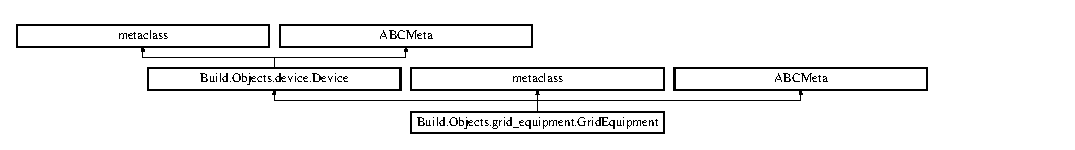
\includegraphics[height=1.561338cm]{class_build_1_1_objects_1_1grid__equipment_1_1_grid_equipment}
\end{center}
\end{figure}
\subsection*{Public Member Functions}
\begin{DoxyCompactItemize}
\item 
def \hyperlink{class_build_1_1_objects_1_1grid__equipment_1_1_grid_equipment_ad25af93202f0bb0c326516f4725b92a8}{\+\_\+\+\_\+init\+\_\+\+\_\+} (self, device\+\_\+id, device\+\_\+type, supervisor, time=0, msg\+\_\+latency=0, schedule=None, multiday=0, total\+\_\+runtime=S\+E\+C\+O\+N\+D\+S\+\_\+\+I\+N\+\_\+\+D\+AY, connected\+\_\+devices=None)
\begin{DoxyCompactList}\small\item\em Initializes a device class with the identical input parameters. \end{DoxyCompactList}\end{DoxyCompactItemize}


\subsection{Constructor \& Destructor Documentation}
\mbox{\Hypertarget{class_build_1_1_objects_1_1grid__equipment_1_1_grid_equipment_ad25af93202f0bb0c326516f4725b92a8}\label{class_build_1_1_objects_1_1grid__equipment_1_1_grid_equipment_ad25af93202f0bb0c326516f4725b92a8}} 
\index{Build\+::\+Objects\+::grid\+\_\+equipment\+::\+Grid\+Equipment@{Build\+::\+Objects\+::grid\+\_\+equipment\+::\+Grid\+Equipment}!\+\_\+\+\_\+init\+\_\+\+\_\+@{\+\_\+\+\_\+init\+\_\+\+\_\+}}
\index{\+\_\+\+\_\+init\+\_\+\+\_\+@{\+\_\+\+\_\+init\+\_\+\+\_\+}!Build\+::\+Objects\+::grid\+\_\+equipment\+::\+Grid\+Equipment@{Build\+::\+Objects\+::grid\+\_\+equipment\+::\+Grid\+Equipment}}
\subsubsection{\texorpdfstring{\+\_\+\+\_\+init\+\_\+\+\_\+()}{\_\_init\_\_()}}
{\footnotesize\ttfamily def Build.\+Objects.\+grid\+\_\+equipment.\+Grid\+Equipment.\+\_\+\+\_\+init\+\_\+\+\_\+ (\begin{DoxyParamCaption}\item[{}]{self,  }\item[{}]{device\+\_\+id,  }\item[{}]{device\+\_\+type,  }\item[{}]{supervisor,  }\item[{}]{time = {\ttfamily 0},  }\item[{}]{msg\+\_\+latency = {\ttfamily 0},  }\item[{}]{schedule = {\ttfamily None},  }\item[{}]{multiday = {\ttfamily 0},  }\item[{}]{total\+\_\+runtime = {\ttfamily SECONDS\+\_\+IN\+\_\+DAY},  }\item[{}]{connected\+\_\+devices = {\ttfamily None} }\end{DoxyParamCaption})}



Initializes a device class with the identical input parameters. 

This will still be an abstract class. 

The documentation for this class was generated from the following file\+:\begin{DoxyCompactItemize}
\item 
Build/\+Objects/grid\+\_\+equipment.\+py\end{DoxyCompactItemize}

\hypertarget{class_build_1_1_objects_1_1light_1_1_light}{}\section{Build.\+Objects.\+light.\+Light Class Reference}
\label{class_build_1_1_objects_1_1light_1_1_light}\index{Build.\+Objects.\+light.\+Light@{Build.\+Objects.\+light.\+Light}}
Inheritance diagram for Build.\+Objects.\+light.\+Light\+:\begin{figure}[H]
\begin{center}
\leavevmode
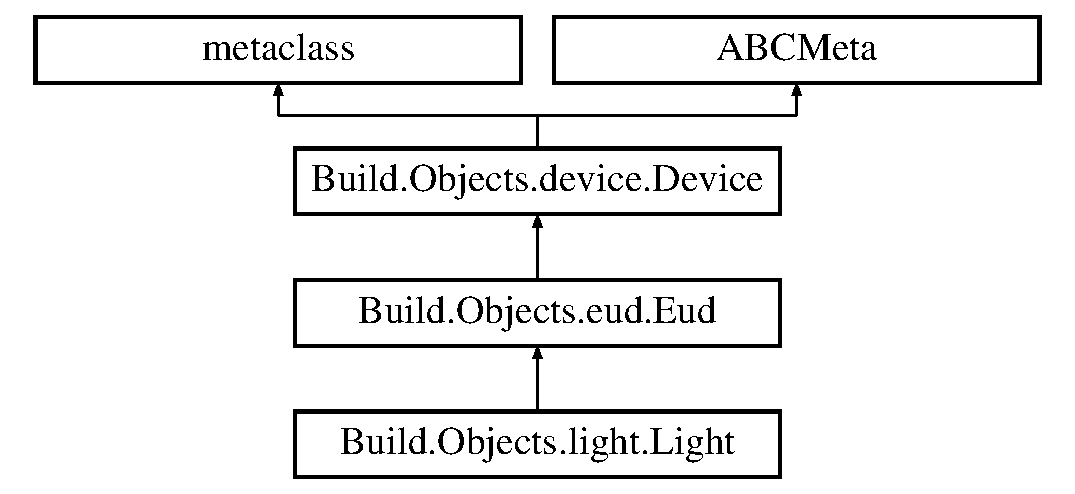
\includegraphics[height=4.000000cm]{class_build_1_1_objects_1_1light_1_1_light}
\end{center}
\end{figure}
\subsection*{Public Member Functions}
\begin{DoxyCompactItemize}
\item 
\mbox{\Hypertarget{class_build_1_1_objects_1_1light_1_1_light_a72d9ed200ef7c129ebff92ffffe2104f}\label{class_build_1_1_objects_1_1light_1_1_light_a72d9ed200ef7c129ebff92ffffe2104f}} 
def {\bfseries \+\_\+\+\_\+init\+\_\+\+\_\+} (self, device\+\_\+id, supervisor, total\+\_\+runtime=S\+E\+C\+O\+N\+D\+S\+\_\+\+I\+N\+\_\+\+D\+AY, multiday=0, modulation\+\_\+interval=7200, msg\+\_\+latency=0, time=0, schedule=None, connected\+\_\+devices=None, max\+\_\+operating\+\_\+power=100.\+0, power\+\_\+level\+\_\+max=1.\+0, power\+\_\+level\+\_\+low=0.\+2, price\+\_\+dim\+\_\+start=0.\+1, price\+\_\+dim\+\_\+end=0.\+2, price\+\_\+off=0.\+3)
\item 
def \hyperlink{class_build_1_1_objects_1_1light_1_1_light_ab2bf34ef61021a564a4be74f618453ce}{calculate\+\_\+desired\+\_\+power\+\_\+level} (self)
\begin{DoxyCompactList}\small\item\em Calculate the desired power level in based on the price (watts). \end{DoxyCompactList}\item 
def \hyperlink{class_build_1_1_objects_1_1light_1_1_light_a12a3c2afe2f8f97aa1d5e28da9059c4e}{on} (self)
\begin{DoxyCompactList}\small\item\em Turns the light \char`\"{}on\char`\"{}, and hence begins consuming power. \end{DoxyCompactList}\item 
def \hyperlink{class_build_1_1_objects_1_1light_1_1_light_a1a7479e6107f3aa664936a234d66c689}{off} (self)
\begin{DoxyCompactList}\small\item\em Turns the light \char`\"{}off\char`\"{}, and stops consuming power. \end{DoxyCompactList}\item 
def \hyperlink{class_build_1_1_objects_1_1light_1_1_light_aabf8b9ee88178489130e5e612d22f7d0}{respond\+\_\+to\+\_\+power} (self, received\+\_\+power)
\begin{DoxyCompactList}\small\item\em The light modulates its brightness based on how much power is received. \end{DoxyCompactList}\item 
\mbox{\Hypertarget{class_build_1_1_objects_1_1light_1_1_light_a2658c7e30fc3fa388033e2bb4ff14442}\label{class_build_1_1_objects_1_1light_1_1_light_a2658c7e30fc3fa388033e2bb4ff14442}} 
def \hyperlink{class_build_1_1_objects_1_1light_1_1_light_a2658c7e30fc3fa388033e2bb4ff14442}{update\+\_\+state} (self)
\begin{DoxyCompactList}\small\item\em \hyperlink{class_build_1_1_objects_1_1light_1_1_light}{Light} does not change dynamic state. \end{DoxyCompactList}\item 
def \hyperlink{class_build_1_1_objects_1_1light_1_1_light_ad11a8dcdfa51caa4133e2e3b68ee2e3f}{begin\+\_\+internal\+\_\+operation} (self)
\begin{DoxyCompactList}\small\item\em \hyperlink{class_build_1_1_objects_1_1light_1_1_light}{Light} does not have a dynamic internal operation. \end{DoxyCompactList}\item 
def \hyperlink{class_build_1_1_objects_1_1light_1_1_light_a42cd8cee6c1f83d8ef053f095f852056}{end\+\_\+internal\+\_\+operation} (self)
\begin{DoxyCompactList}\small\item\em \hyperlink{class_build_1_1_objects_1_1light_1_1_light}{Light} does not have a dynamic internal operation. \end{DoxyCompactList}\item 
def \hyperlink{class_build_1_1_objects_1_1light_1_1_light_a5b2b078fd97d8bc80262f57d1e97377d}{device\+\_\+specific\+\_\+calcs} (self)
\begin{DoxyCompactList}\small\item\em \hyperlink{class_build_1_1_objects_1_1light_1_1_light}{Light} does not have extra calculations beyond power consumption. \end{DoxyCompactList}\end{DoxyCompactItemize}
\subsection*{Additional Inherited Members}


\subsection{Member Function Documentation}
\mbox{\Hypertarget{class_build_1_1_objects_1_1light_1_1_light_ad11a8dcdfa51caa4133e2e3b68ee2e3f}\label{class_build_1_1_objects_1_1light_1_1_light_ad11a8dcdfa51caa4133e2e3b68ee2e3f}} 
\index{Build\+::\+Objects\+::light\+::\+Light@{Build\+::\+Objects\+::light\+::\+Light}!begin\+\_\+internal\+\_\+operation@{begin\+\_\+internal\+\_\+operation}}
\index{begin\+\_\+internal\+\_\+operation@{begin\+\_\+internal\+\_\+operation}!Build\+::\+Objects\+::light\+::\+Light@{Build\+::\+Objects\+::light\+::\+Light}}
\subsubsection{\texorpdfstring{begin\+\_\+internal\+\_\+operation()}{begin\_internal\_operation()}}
{\footnotesize\ttfamily def Build.\+Objects.\+light.\+Light.\+begin\+\_\+internal\+\_\+operation (\begin{DoxyParamCaption}\item[{}]{self }\end{DoxyParamCaption})}



\hyperlink{class_build_1_1_objects_1_1light_1_1_light}{Light} does not have a dynamic internal operation. 

\mbox{\Hypertarget{class_build_1_1_objects_1_1light_1_1_light_ab2bf34ef61021a564a4be74f618453ce}\label{class_build_1_1_objects_1_1light_1_1_light_ab2bf34ef61021a564a4be74f618453ce}} 
\index{Build\+::\+Objects\+::light\+::\+Light@{Build\+::\+Objects\+::light\+::\+Light}!calculate\+\_\+desired\+\_\+power\+\_\+level@{calculate\+\_\+desired\+\_\+power\+\_\+level}}
\index{calculate\+\_\+desired\+\_\+power\+\_\+level@{calculate\+\_\+desired\+\_\+power\+\_\+level}!Build\+::\+Objects\+::light\+::\+Light@{Build\+::\+Objects\+::light\+::\+Light}}
\subsubsection{\texorpdfstring{calculate\+\_\+desired\+\_\+power\+\_\+level()}{calculate\_desired\_power\_level()}}
{\footnotesize\ttfamily def Build.\+Objects.\+light.\+Light.\+calculate\+\_\+desired\+\_\+power\+\_\+level (\begin{DoxyParamCaption}\item[{}]{self }\end{DoxyParamCaption})}



Calculate the desired power level in based on the price (watts). 

Algorithm is described in software documentation. \mbox{\Hypertarget{class_build_1_1_objects_1_1light_1_1_light_a5b2b078fd97d8bc80262f57d1e97377d}\label{class_build_1_1_objects_1_1light_1_1_light_a5b2b078fd97d8bc80262f57d1e97377d}} 
\index{Build\+::\+Objects\+::light\+::\+Light@{Build\+::\+Objects\+::light\+::\+Light}!device\+\_\+specific\+\_\+calcs@{device\+\_\+specific\+\_\+calcs}}
\index{device\+\_\+specific\+\_\+calcs@{device\+\_\+specific\+\_\+calcs}!Build\+::\+Objects\+::light\+::\+Light@{Build\+::\+Objects\+::light\+::\+Light}}
\subsubsection{\texorpdfstring{device\+\_\+specific\+\_\+calcs()}{device\_specific\_calcs()}}
{\footnotesize\ttfamily def Build.\+Objects.\+light.\+Light.\+device\+\_\+specific\+\_\+calcs (\begin{DoxyParamCaption}\item[{}]{self }\end{DoxyParamCaption})}



\hyperlink{class_build_1_1_objects_1_1light_1_1_light}{Light} does not have extra calculations beyond power consumption. 

\mbox{\Hypertarget{class_build_1_1_objects_1_1light_1_1_light_a42cd8cee6c1f83d8ef053f095f852056}\label{class_build_1_1_objects_1_1light_1_1_light_a42cd8cee6c1f83d8ef053f095f852056}} 
\index{Build\+::\+Objects\+::light\+::\+Light@{Build\+::\+Objects\+::light\+::\+Light}!end\+\_\+internal\+\_\+operation@{end\+\_\+internal\+\_\+operation}}
\index{end\+\_\+internal\+\_\+operation@{end\+\_\+internal\+\_\+operation}!Build\+::\+Objects\+::light\+::\+Light@{Build\+::\+Objects\+::light\+::\+Light}}
\subsubsection{\texorpdfstring{end\+\_\+internal\+\_\+operation()}{end\_internal\_operation()}}
{\footnotesize\ttfamily def Build.\+Objects.\+light.\+Light.\+end\+\_\+internal\+\_\+operation (\begin{DoxyParamCaption}\item[{}]{self }\end{DoxyParamCaption})}



\hyperlink{class_build_1_1_objects_1_1light_1_1_light}{Light} does not have a dynamic internal operation. 

\mbox{\Hypertarget{class_build_1_1_objects_1_1light_1_1_light_a1a7479e6107f3aa664936a234d66c689}\label{class_build_1_1_objects_1_1light_1_1_light_a1a7479e6107f3aa664936a234d66c689}} 
\index{Build\+::\+Objects\+::light\+::\+Light@{Build\+::\+Objects\+::light\+::\+Light}!off@{off}}
\index{off@{off}!Build\+::\+Objects\+::light\+::\+Light@{Build\+::\+Objects\+::light\+::\+Light}}
\subsubsection{\texorpdfstring{off()}{off()}}
{\footnotesize\ttfamily def Build.\+Objects.\+light.\+Light.\+off (\begin{DoxyParamCaption}\item[{}]{self }\end{DoxyParamCaption})}



Turns the light \char`\"{}off\char`\"{}, and stops consuming power. 

Does not affect this device\textquotesingle{}s ability to receive messages, and it remains in operation even when off. \mbox{\Hypertarget{class_build_1_1_objects_1_1light_1_1_light_a12a3c2afe2f8f97aa1d5e28da9059c4e}\label{class_build_1_1_objects_1_1light_1_1_light_a12a3c2afe2f8f97aa1d5e28da9059c4e}} 
\index{Build\+::\+Objects\+::light\+::\+Light@{Build\+::\+Objects\+::light\+::\+Light}!on@{on}}
\index{on@{on}!Build\+::\+Objects\+::light\+::\+Light@{Build\+::\+Objects\+::light\+::\+Light}}
\subsubsection{\texorpdfstring{on()}{on()}}
{\footnotesize\ttfamily def Build.\+Objects.\+light.\+Light.\+on (\begin{DoxyParamCaption}\item[{}]{self }\end{DoxyParamCaption})}



Turns the light \char`\"{}on\char`\"{}, and hence begins consuming power. 

Does not affect whether device is in operation and can receive messages, only power consumption. \mbox{\Hypertarget{class_build_1_1_objects_1_1light_1_1_light_aabf8b9ee88178489130e5e612d22f7d0}\label{class_build_1_1_objects_1_1light_1_1_light_aabf8b9ee88178489130e5e612d22f7d0}} 
\index{Build\+::\+Objects\+::light\+::\+Light@{Build\+::\+Objects\+::light\+::\+Light}!respond\+\_\+to\+\_\+power@{respond\+\_\+to\+\_\+power}}
\index{respond\+\_\+to\+\_\+power@{respond\+\_\+to\+\_\+power}!Build\+::\+Objects\+::light\+::\+Light@{Build\+::\+Objects\+::light\+::\+Light}}
\subsubsection{\texorpdfstring{respond\+\_\+to\+\_\+power()}{respond\_to\_power()}}
{\footnotesize\ttfamily def Build.\+Objects.\+light.\+Light.\+respond\+\_\+to\+\_\+power (\begin{DoxyParamCaption}\item[{}]{self,  }\item[{}]{received\+\_\+power }\end{DoxyParamCaption})}



The light modulates its brightness based on how much power is received. 

Brightness is ratio of received power to maximum operating power. 
\begin{DoxyParams}{Parameters}
{\em received\+\_\+power} & how much power this light received to operate \\
\hline
\end{DoxyParams}


The documentation for this class was generated from the following file\+:\begin{DoxyCompactItemize}
\item 
Build/\+Objects/light.\+py\end{DoxyCompactItemize}

\hypertarget{class_build_1_1_simulation___operation_1_1message_1_1_message}{}\section{Build.\+Simulation\+\_\+\+Operation.\+message.\+Message Class Reference}
\label{class_build_1_1_simulation___operation_1_1message_1_1_message}\index{Build.\+Simulation\+\_\+\+Operation.\+message.\+Message@{Build.\+Simulation\+\_\+\+Operation.\+message.\+Message}}
Inheritance diagram for Build.\+Simulation\+\_\+\+Operation.\+message.\+Message\+:\begin{figure}[H]
\begin{center}
\leavevmode
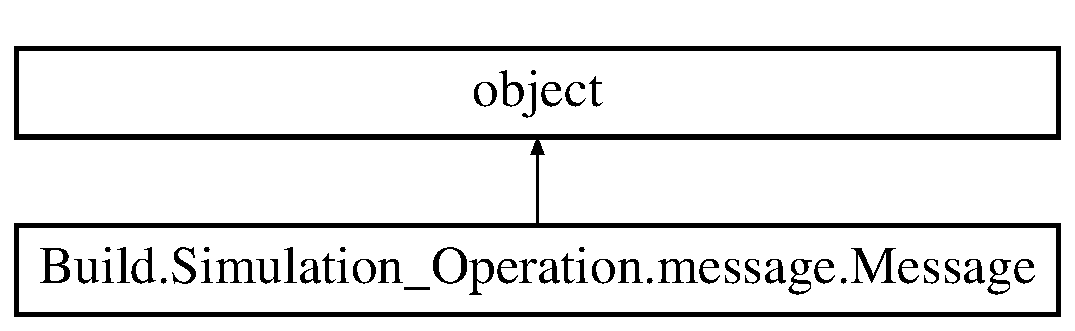
\includegraphics[height=2.000000cm]{class_build_1_1_simulation___operation_1_1message_1_1_message}
\end{center}
\end{figure}
\subsection*{Public Member Functions}
\begin{DoxyCompactItemize}
\item 
\mbox{\Hypertarget{class_build_1_1_simulation___operation_1_1message_1_1_message_ad36dcd76b28ea97a3b1c454feb5317e2}\label{class_build_1_1_simulation___operation_1_1message_1_1_message_ad36dcd76b28ea97a3b1c454feb5317e2}} 
def {\bfseries \+\_\+\+\_\+init\+\_\+\+\_\+} (self, time, sender\+\_\+id, message\+\_\+type, value, extra\+\_\+info=None)
\end{DoxyCompactItemize}
\subsection*{Public Attributes}
\begin{DoxyCompactItemize}
\item 
\mbox{\Hypertarget{class_build_1_1_simulation___operation_1_1message_1_1_message_a6122da2afc91c2fd23519a8c38343217}\label{class_build_1_1_simulation___operation_1_1message_1_1_message_a6122da2afc91c2fd23519a8c38343217}} 
{\bfseries time}
\item 
\mbox{\Hypertarget{class_build_1_1_simulation___operation_1_1message_1_1_message_af9430f21634626fd9497430b21f5b41a}\label{class_build_1_1_simulation___operation_1_1message_1_1_message_af9430f21634626fd9497430b21f5b41a}} 
{\bfseries sender\+\_\+id}
\item 
\mbox{\Hypertarget{class_build_1_1_simulation___operation_1_1message_1_1_message_aa05203803421b175e29735ccb37a0dad}\label{class_build_1_1_simulation___operation_1_1message_1_1_message_aa05203803421b175e29735ccb37a0dad}} 
{\bfseries message\+\_\+type}
\item 
\mbox{\Hypertarget{class_build_1_1_simulation___operation_1_1message_1_1_message_ac09cc0f69cce74d44a670f649fb89cc4}\label{class_build_1_1_simulation___operation_1_1message_1_1_message_ac09cc0f69cce74d44a670f649fb89cc4}} 
{\bfseries value}
\item 
\mbox{\Hypertarget{class_build_1_1_simulation___operation_1_1message_1_1_message_ad1acb28de8d98f557bc0d98b8a641fba}\label{class_build_1_1_simulation___operation_1_1message_1_1_message_ad1acb28de8d98f557bc0d98b8a641fba}} 
{\bfseries extra\+\_\+info}
\end{DoxyCompactItemize}


The documentation for this class was generated from the following file\+:\begin{DoxyCompactItemize}
\item 
Build/\+Simulation\+\_\+\+Operation/message.\+py\end{DoxyCompactItemize}

\hypertarget{class_build_1_1_simulation___operation_1_1message_1_1_message_type}{}\section{Build.\+Simulation\+\_\+\+Operation.\+message.\+Message\+Type Class Reference}
\label{class_build_1_1_simulation___operation_1_1message_1_1_message_type}\index{Build.\+Simulation\+\_\+\+Operation.\+message.\+Message\+Type@{Build.\+Simulation\+\_\+\+Operation.\+message.\+Message\+Type}}


Messages can be of five types\+: Register, power, price, request, and allocate.  


Inheritance diagram for Build.\+Simulation\+\_\+\+Operation.\+message.\+Message\+Type\+:\begin{figure}[H]
\begin{center}
\leavevmode
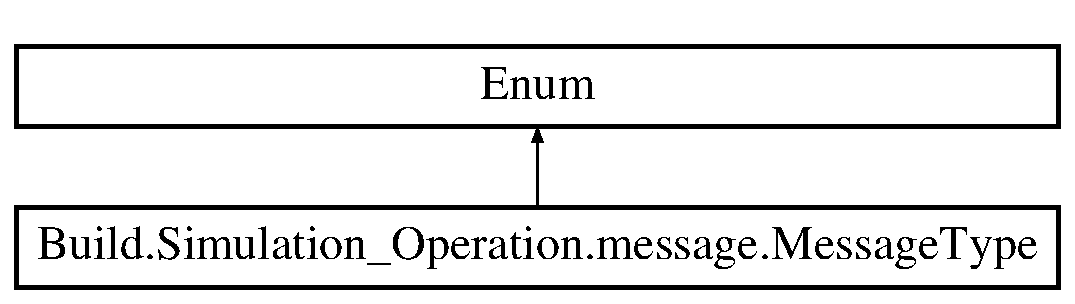
\includegraphics[height=2.000000cm]{class_build_1_1_simulation___operation_1_1message_1_1_message_type}
\end{center}
\end{figure}
\subsection*{Static Public Attributes}
\begin{DoxyCompactItemize}
\item 
\mbox{\Hypertarget{class_build_1_1_simulation___operation_1_1message_1_1_message_type_a518eb650dfc94f31142b07f0caa5ac09}\label{class_build_1_1_simulation___operation_1_1message_1_1_message_type_a518eb650dfc94f31142b07f0caa5ac09}} 
int {\bfseries R\+E\+G\+I\+S\+T\+ER} = 1
\item 
\mbox{\Hypertarget{class_build_1_1_simulation___operation_1_1message_1_1_message_type_abc56c6f1776929c18f8b6fc8b74001fe}\label{class_build_1_1_simulation___operation_1_1message_1_1_message_type_abc56c6f1776929c18f8b6fc8b74001fe}} 
int {\bfseries P\+O\+W\+ER} = 2
\item 
\mbox{\Hypertarget{class_build_1_1_simulation___operation_1_1message_1_1_message_type_a68afec66af746b54718007bf8d059943}\label{class_build_1_1_simulation___operation_1_1message_1_1_message_type_a68afec66af746b54718007bf8d059943}} 
int {\bfseries P\+R\+I\+CE} = 3
\item 
\mbox{\Hypertarget{class_build_1_1_simulation___operation_1_1message_1_1_message_type_a60bbbb6d2d9a92e2021e20485288c011}\label{class_build_1_1_simulation___operation_1_1message_1_1_message_type_a60bbbb6d2d9a92e2021e20485288c011}} 
int {\bfseries R\+E\+Q\+U\+E\+ST} = 4
\item 
\mbox{\Hypertarget{class_build_1_1_simulation___operation_1_1message_1_1_message_type_aa0b29a936d5282d2da064604df74db7b}\label{class_build_1_1_simulation___operation_1_1message_1_1_message_type_aa0b29a936d5282d2da064604df74db7b}} 
int {\bfseries A\+L\+L\+O\+C\+A\+TE} = 5
\end{DoxyCompactItemize}


\subsection{Detailed Description}
Messages can be of five types\+: Register, power, price, request, and allocate. 

A register message indicates that a device is seeking to register or unregister a connection with another device; a positive value with Register indicates that it would like to be registered under that device\textquotesingle{}s connected devices, while a negative value indicates that it is requesting to disconnect.

A power message informs another device that power is now flowing between them in a certain direction. Once a device has received a power message with a certain quantity, that power flow must now exists between them -- there is no further negotiation. 

The documentation for this class was generated from the following file\+:\begin{DoxyCompactItemize}
\item 
Build/\+Simulation\+\_\+\+Operation/message.\+py\end{DoxyCompactItemize}

\hypertarget{class_build_1_1_simulation___operation_1_1queue_1_1_priority_queue}{}\section{Build.\+Simulation\+\_\+\+Operation.\+queue.\+Priority\+Queue Class Reference}
\label{class_build_1_1_simulation___operation_1_1queue_1_1_priority_queue}\index{Build.\+Simulation\+\_\+\+Operation.\+queue.\+Priority\+Queue@{Build.\+Simulation\+\_\+\+Operation.\+queue.\+Priority\+Queue}}
\subsection*{Public Member Functions}
\begin{DoxyCompactItemize}
\item 
\mbox{\Hypertarget{class_build_1_1_simulation___operation_1_1queue_1_1_priority_queue_aee409aeb79269e2167c83cecdd3b2db2}\label{class_build_1_1_simulation___operation_1_1queue_1_1_priority_queue_aee409aeb79269e2167c83cecdd3b2db2}} 
def {\bfseries \+\_\+\+\_\+init\+\_\+\+\_\+} (self)
\item 
def \hyperlink{class_build_1_1_simulation___operation_1_1queue_1_1_priority_queue_a042956dd1eaf2317965630e8deed80b3}{add} (self, task, priority=0)
\begin{DoxyCompactList}\small\item\em Adds a new task to the priority queue, or if that task already exists, updates that tasks priority. \end{DoxyCompactList}\item 
def \hyperlink{class_build_1_1_simulation___operation_1_1queue_1_1_priority_queue_af953e022ce390c5090ebe7de4f1ea6ec}{update\+\_\+by\+\_\+attribute} (self, task\+\_\+attribute, attribute\+\_\+value, new\+\_\+priority=0)
\begin{DoxyCompactList}\small\item\em Updates all tasks with a given task\+\_\+attribute equal to an attribute\+\_\+value to have a new priority. \end{DoxyCompactList}\item 
def \hyperlink{class_build_1_1_simulation___operation_1_1queue_1_1_priority_queue_a86faaf2d1f76eb146b6e1d5a55df09ba}{remove} (self, task)
\begin{DoxyCompactList}\small\item\em Marks an existing task as R\+E\+M\+O\+V\+ED in the heap. \end{DoxyCompactList}\item 
def \hyperlink{class_build_1_1_simulation___operation_1_1queue_1_1_priority_queue_aff0c9a1aefbac68dd00cb274adb1d739}{pop} (self)
\begin{DoxyCompactList}\small\item\em Remove and return the lowest priority task and its priority. \end{DoxyCompactList}\item 
def \hyperlink{class_build_1_1_simulation___operation_1_1queue_1_1_priority_queue_aae2cb79110fbe3917ede657052bb3976}{peek} (self)
\begin{DoxyCompactList}\small\item\em Returns the lowest priority task in the queue and its priority without removing. \end{DoxyCompactList}\item 
def \hyperlink{class_build_1_1_simulation___operation_1_1queue_1_1_priority_queue_a62ca97541bd2863177111afa2ebf01f0}{is\+\_\+empty} (self)
\begin{DoxyCompactList}\small\item\em Returns whether the queue is empty. \end{DoxyCompactList}\item 
def \hyperlink{class_build_1_1_simulation___operation_1_1queue_1_1_priority_queue_aeac0d1993374ae61b482b14cfe824473}{clear} (self)
\begin{DoxyCompactList}\small\item\em Clears out all values from the priority queue. \end{DoxyCompactList}\end{DoxyCompactItemize}
\subsection*{Static Public Attributes}
\begin{DoxyCompactItemize}
\item 
\mbox{\Hypertarget{class_build_1_1_simulation___operation_1_1queue_1_1_priority_queue_add1fdf8c2db1431d3368ca1f9a1b56e6}\label{class_build_1_1_simulation___operation_1_1queue_1_1_priority_queue_add1fdf8c2db1431d3368ca1f9a1b56e6}} 
string {\bfseries R\+E\+M\+O\+V\+ED} = \textquotesingle{}$<$removed-\/task$>$\textquotesingle{}
\end{DoxyCompactItemize}


\subsection{Member Function Documentation}
\mbox{\Hypertarget{class_build_1_1_simulation___operation_1_1queue_1_1_priority_queue_a042956dd1eaf2317965630e8deed80b3}\label{class_build_1_1_simulation___operation_1_1queue_1_1_priority_queue_a042956dd1eaf2317965630e8deed80b3}} 
\index{Build\+::\+Simulation\+\_\+\+Operation\+::queue\+::\+Priority\+Queue@{Build\+::\+Simulation\+\_\+\+Operation\+::queue\+::\+Priority\+Queue}!add@{add}}
\index{add@{add}!Build\+::\+Simulation\+\_\+\+Operation\+::queue\+::\+Priority\+Queue@{Build\+::\+Simulation\+\_\+\+Operation\+::queue\+::\+Priority\+Queue}}
\subsubsection{\texorpdfstring{add()}{add()}}
{\footnotesize\ttfamily def Build.\+Simulation\+\_\+\+Operation.\+queue.\+Priority\+Queue.\+add (\begin{DoxyParamCaption}\item[{}]{self,  }\item[{}]{task,  }\item[{}]{priority = {\ttfamily 0} }\end{DoxyParamCaption})}



Adds a new task to the priority queue, or if that task already exists, updates that tasks priority. 


\begin{DoxyParams}{Parameters}
{\em task} & the task to add to the priority queue \\
\hline
{\em priority} & the priority to assign to this task. Default to 0 \\
\hline
\end{DoxyParams}
\mbox{\Hypertarget{class_build_1_1_simulation___operation_1_1queue_1_1_priority_queue_aeac0d1993374ae61b482b14cfe824473}\label{class_build_1_1_simulation___operation_1_1queue_1_1_priority_queue_aeac0d1993374ae61b482b14cfe824473}} 
\index{Build\+::\+Simulation\+\_\+\+Operation\+::queue\+::\+Priority\+Queue@{Build\+::\+Simulation\+\_\+\+Operation\+::queue\+::\+Priority\+Queue}!clear@{clear}}
\index{clear@{clear}!Build\+::\+Simulation\+\_\+\+Operation\+::queue\+::\+Priority\+Queue@{Build\+::\+Simulation\+\_\+\+Operation\+::queue\+::\+Priority\+Queue}}
\subsubsection{\texorpdfstring{clear()}{clear()}}
{\footnotesize\ttfamily def Build.\+Simulation\+\_\+\+Operation.\+queue.\+Priority\+Queue.\+clear (\begin{DoxyParamCaption}\item[{}]{self }\end{DoxyParamCaption})}



Clears out all values from the priority queue. 

\begin{DoxyVerb}clear the priority queue\end{DoxyVerb}
 \mbox{\Hypertarget{class_build_1_1_simulation___operation_1_1queue_1_1_priority_queue_a62ca97541bd2863177111afa2ebf01f0}\label{class_build_1_1_simulation___operation_1_1queue_1_1_priority_queue_a62ca97541bd2863177111afa2ebf01f0}} 
\index{Build\+::\+Simulation\+\_\+\+Operation\+::queue\+::\+Priority\+Queue@{Build\+::\+Simulation\+\_\+\+Operation\+::queue\+::\+Priority\+Queue}!is\+\_\+empty@{is\+\_\+empty}}
\index{is\+\_\+empty@{is\+\_\+empty}!Build\+::\+Simulation\+\_\+\+Operation\+::queue\+::\+Priority\+Queue@{Build\+::\+Simulation\+\_\+\+Operation\+::queue\+::\+Priority\+Queue}}
\subsubsection{\texorpdfstring{is\+\_\+empty()}{is\_empty()}}
{\footnotesize\ttfamily def Build.\+Simulation\+\_\+\+Operation.\+queue.\+Priority\+Queue.\+is\+\_\+empty (\begin{DoxyParamCaption}\item[{}]{self }\end{DoxyParamCaption})}



Returns whether the queue is empty. 

\mbox{\Hypertarget{class_build_1_1_simulation___operation_1_1queue_1_1_priority_queue_aae2cb79110fbe3917ede657052bb3976}\label{class_build_1_1_simulation___operation_1_1queue_1_1_priority_queue_aae2cb79110fbe3917ede657052bb3976}} 
\index{Build\+::\+Simulation\+\_\+\+Operation\+::queue\+::\+Priority\+Queue@{Build\+::\+Simulation\+\_\+\+Operation\+::queue\+::\+Priority\+Queue}!peek@{peek}}
\index{peek@{peek}!Build\+::\+Simulation\+\_\+\+Operation\+::queue\+::\+Priority\+Queue@{Build\+::\+Simulation\+\_\+\+Operation\+::queue\+::\+Priority\+Queue}}
\subsubsection{\texorpdfstring{peek()}{peek()}}
{\footnotesize\ttfamily def Build.\+Simulation\+\_\+\+Operation.\+queue.\+Priority\+Queue.\+peek (\begin{DoxyParamCaption}\item[{}]{self }\end{DoxyParamCaption})}



Returns the lowest priority task in the queue and its priority without removing. 

Raise Key\+Error if queue is empty. \begin{DoxyReturn}{Returns}
tuple of task with lowest priority and that priority 
\end{DoxyReturn}
\mbox{\Hypertarget{class_build_1_1_simulation___operation_1_1queue_1_1_priority_queue_aff0c9a1aefbac68dd00cb274adb1d739}\label{class_build_1_1_simulation___operation_1_1queue_1_1_priority_queue_aff0c9a1aefbac68dd00cb274adb1d739}} 
\index{Build\+::\+Simulation\+\_\+\+Operation\+::queue\+::\+Priority\+Queue@{Build\+::\+Simulation\+\_\+\+Operation\+::queue\+::\+Priority\+Queue}!pop@{pop}}
\index{pop@{pop}!Build\+::\+Simulation\+\_\+\+Operation\+::queue\+::\+Priority\+Queue@{Build\+::\+Simulation\+\_\+\+Operation\+::queue\+::\+Priority\+Queue}}
\subsubsection{\texorpdfstring{pop()}{pop()}}
{\footnotesize\ttfamily def Build.\+Simulation\+\_\+\+Operation.\+queue.\+Priority\+Queue.\+pop (\begin{DoxyParamCaption}\item[{}]{self }\end{DoxyParamCaption})}



Remove and return the lowest priority task and its priority. 

Raise Key\+Error if queue is empty. \begin{DoxyReturn}{Returns}
tuple of task with lowest priority and that priority 
\end{DoxyReturn}
\mbox{\Hypertarget{class_build_1_1_simulation___operation_1_1queue_1_1_priority_queue_a86faaf2d1f76eb146b6e1d5a55df09ba}\label{class_build_1_1_simulation___operation_1_1queue_1_1_priority_queue_a86faaf2d1f76eb146b6e1d5a55df09ba}} 
\index{Build\+::\+Simulation\+\_\+\+Operation\+::queue\+::\+Priority\+Queue@{Build\+::\+Simulation\+\_\+\+Operation\+::queue\+::\+Priority\+Queue}!remove@{remove}}
\index{remove@{remove}!Build\+::\+Simulation\+\_\+\+Operation\+::queue\+::\+Priority\+Queue@{Build\+::\+Simulation\+\_\+\+Operation\+::queue\+::\+Priority\+Queue}}
\subsubsection{\texorpdfstring{remove()}{remove()}}
{\footnotesize\ttfamily def Build.\+Simulation\+\_\+\+Operation.\+queue.\+Priority\+Queue.\+remove (\begin{DoxyParamCaption}\item[{}]{self,  }\item[{}]{task }\end{DoxyParamCaption})}



Marks an existing task as R\+E\+M\+O\+V\+ED in the heap. 

When this value is encountered later in a pop or peek, it will be removed for good from the heap. Raises a Key\+Error if that task is not found. \mbox{\Hypertarget{class_build_1_1_simulation___operation_1_1queue_1_1_priority_queue_af953e022ce390c5090ebe7de4f1ea6ec}\label{class_build_1_1_simulation___operation_1_1queue_1_1_priority_queue_af953e022ce390c5090ebe7de4f1ea6ec}} 
\index{Build\+::\+Simulation\+\_\+\+Operation\+::queue\+::\+Priority\+Queue@{Build\+::\+Simulation\+\_\+\+Operation\+::queue\+::\+Priority\+Queue}!update\+\_\+by\+\_\+attribute@{update\+\_\+by\+\_\+attribute}}
\index{update\+\_\+by\+\_\+attribute@{update\+\_\+by\+\_\+attribute}!Build\+::\+Simulation\+\_\+\+Operation\+::queue\+::\+Priority\+Queue@{Build\+::\+Simulation\+\_\+\+Operation\+::queue\+::\+Priority\+Queue}}
\subsubsection{\texorpdfstring{update\+\_\+by\+\_\+attribute()}{update\_by\_attribute()}}
{\footnotesize\ttfamily def Build.\+Simulation\+\_\+\+Operation.\+queue.\+Priority\+Queue.\+update\+\_\+by\+\_\+attribute (\begin{DoxyParamCaption}\item[{}]{self,  }\item[{}]{task\+\_\+attribute,  }\item[{}]{attribute\+\_\+value,  }\item[{}]{new\+\_\+priority = {\ttfamily 0} }\end{DoxyParamCaption})}



Updates all tasks with a given task\+\_\+attribute equal to an attribute\+\_\+value to have a new priority. 


\begin{DoxyParams}{Parameters}
{\em task\+\_\+attribute} & an attribute of the task to identify it \\
\hline
{\em attribute\+\_\+value} & the value of that attribute that we want to isolate \\
\hline
{\em new\+\_\+priority} & the new priority value to assign to the tasks that have the desired attribute value \\
\hline
\end{DoxyParams}


The documentation for this class was generated from the following file\+:\begin{DoxyCompactItemize}
\item 
Build/\+Simulation\+\_\+\+Operation/queue.\+py\end{DoxyCompactItemize}

\hypertarget{class_build_1_1_objects_1_1pv_1_1_p_v}{}\section{Build.\+Objects.\+pv.\+PV Class Reference}
\label{class_build_1_1_objects_1_1pv_1_1_p_v}\index{Build.\+Objects.\+pv.\+PV@{Build.\+Objects.\+pv.\+PV}}
Inheritance diagram for Build.\+Objects.\+pv.\+PV\+:\begin{figure}[H]
\begin{center}
\leavevmode
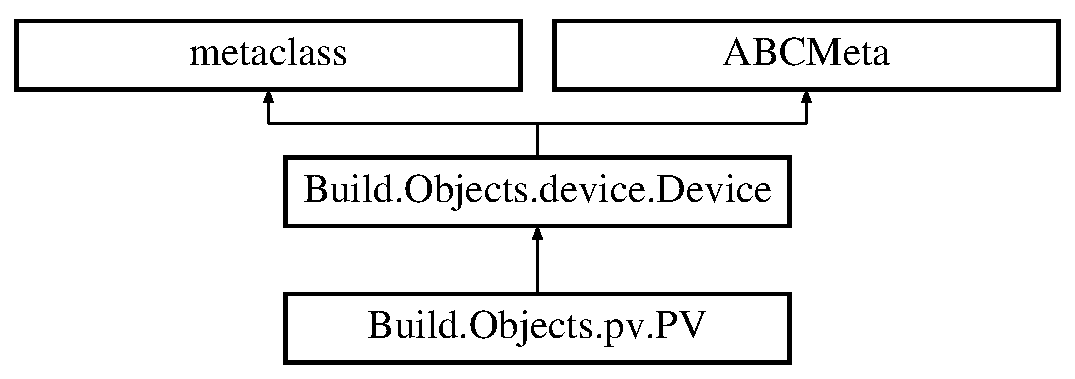
\includegraphics[height=3.000000cm]{class_build_1_1_objects_1_1pv_1_1_p_v}
\end{center}
\end{figure}
\subsection*{Public Member Functions}
\begin{DoxyCompactItemize}
\item 
\mbox{\Hypertarget{class_build_1_1_objects_1_1pv_1_1_p_v_ab85f5c9b0dbc579445834b47f344e9d7}\label{class_build_1_1_objects_1_1pv_1_1_p_v_ab85f5c9b0dbc579445834b47f344e9d7}} 
def {\bfseries \+\_\+\+\_\+init\+\_\+\+\_\+} (self, device\+\_\+id, supervisor, power\+\_\+profile, peak\+\_\+power, time=0, msg\+\_\+latency=0, schedule=None, connected\+\_\+devices=None, total\+\_\+runtime=S\+E\+C\+O\+N\+D\+S\+\_\+\+I\+N\+\_\+\+D\+AY)
\item 
def \hyperlink{class_build_1_1_objects_1_1pv_1_1_p_v_a8c06b93d9d13ee9b6991c3b498bf469e}{setup\+\_\+power\+\_\+schedule} (self, power\+\_\+profile, peak\+\_\+power, total\+\_\+runtime)
\begin{DoxyCompactList}\small\item\em Sets up the power generation schedule for this \hyperlink{class_build_1_1_objects_1_1pv_1_1_p_v}{PV}. \end{DoxyCompactList}\item 
def \hyperlink{class_build_1_1_objects_1_1pv_1_1_p_v_a0c27298b51f1e227cee28bb3f6528742}{update\+\_\+power\+\_\+status} (self, peak\+\_\+power, power\+\_\+percent)
\begin{DoxyCompactList}\small\item\em Changes the amount of power that this device is producing and If this \hyperlink{class_build_1_1_objects_1_1pv_1_1_p_v}{PV} is connected to multiple devices, it evenly distributes its load amongst them. \end{DoxyCompactList}\item 
\mbox{\Hypertarget{class_build_1_1_objects_1_1pv_1_1_p_v_acbeb8820230c1c317e553db544b38286}\label{class_build_1_1_objects_1_1pv_1_1_p_v_acbeb8820230c1c317e553db544b38286}} 
def \hyperlink{class_build_1_1_objects_1_1pv_1_1_p_v_acbeb8820230c1c317e553db544b38286}{send\+\_\+power\+\_\+message} (self, target\+\_\+id, power\+\_\+amt)
\begin{DoxyCompactList}\small\item\em This \hyperlink{class_build_1_1_objects_1_1pv_1_1_p_v}{PV} will provide the power it , informing another device of the quantity by. \end{DoxyCompactList}\item 
def \hyperlink{class_build_1_1_objects_1_1pv_1_1_p_v_a4e7810d5ba27d6414abca31af54d8949}{process\+\_\+power\+\_\+message} (self, sender\+\_\+id, new\+\_\+power)
\begin{DoxyCompactList}\small\item\em \hyperlink{class_build_1_1_objects_1_1pv_1_1_p_v}{PV} does not respond to external power messages. \end{DoxyCompactList}\item 
def \hyperlink{class_build_1_1_objects_1_1pv_1_1_p_v_a5f41b238d5d48ac989782e1c6fffaa54}{process\+\_\+price\+\_\+message} (self, sender\+\_\+id, new\+\_\+price, extra\+\_\+info)
\begin{DoxyCompactList}\small\item\em \hyperlink{class_build_1_1_objects_1_1pv_1_1_p_v}{PV} does not respond to price information. \end{DoxyCompactList}\item 
def \hyperlink{class_build_1_1_objects_1_1pv_1_1_p_v_ab560ae3ebbbb4c57382daa39d39fe654}{process\+\_\+request\+\_\+message} (self, sender\+\_\+id, request\+\_\+amt)
\begin{DoxyCompactList}\small\item\em \hyperlink{class_build_1_1_objects_1_1pv_1_1_p_v}{PV} does not respond to request information. \end{DoxyCompactList}\item 
def \hyperlink{class_build_1_1_objects_1_1pv_1_1_p_v_aabdf52b13172ff2c632d7f7cde732191}{process\+\_\+allocate\+\_\+message} (self, sender\+\_\+id, allocate\+\_\+amt)
\begin{DoxyCompactList}\small\item\em \hyperlink{class_build_1_1_objects_1_1pv_1_1_p_v}{PV} does not respond to allocate messages. \end{DoxyCompactList}\item 
\mbox{\Hypertarget{class_build_1_1_objects_1_1pv_1_1_p_v_a6ef12cbd9bbcaeba45203b355d434b81}\label{class_build_1_1_objects_1_1pv_1_1_p_v_a6ef12cbd9bbcaeba45203b355d434b81}} 
def \hyperlink{class_build_1_1_objects_1_1pv_1_1_p_v_a6ef12cbd9bbcaeba45203b355d434b81}{device\+\_\+specific\+\_\+calcs} (self)
\begin{DoxyCompactList}\small\item\em \hyperlink{class_build_1_1_objects_1_1pv_1_1_p_v}{PV} does not calculate any new usage information besides sum power out. \end{DoxyCompactList}\end{DoxyCompactItemize}


\subsection{Member Function Documentation}
\mbox{\Hypertarget{class_build_1_1_objects_1_1pv_1_1_p_v_aabdf52b13172ff2c632d7f7cde732191}\label{class_build_1_1_objects_1_1pv_1_1_p_v_aabdf52b13172ff2c632d7f7cde732191}} 
\index{Build\+::\+Objects\+::pv\+::\+PV@{Build\+::\+Objects\+::pv\+::\+PV}!process\+\_\+allocate\+\_\+message@{process\+\_\+allocate\+\_\+message}}
\index{process\+\_\+allocate\+\_\+message@{process\+\_\+allocate\+\_\+message}!Build\+::\+Objects\+::pv\+::\+PV@{Build\+::\+Objects\+::pv\+::\+PV}}
\subsubsection{\texorpdfstring{process\+\_\+allocate\+\_\+message()}{process\_allocate\_message()}}
{\footnotesize\ttfamily def Build.\+Objects.\+pv.\+P\+V.\+process\+\_\+allocate\+\_\+message (\begin{DoxyParamCaption}\item[{}]{self,  }\item[{}]{sender\+\_\+id,  }\item[{}]{allocate\+\_\+amt }\end{DoxyParamCaption})}



\hyperlink{class_build_1_1_objects_1_1pv_1_1_p_v}{PV} does not respond to allocate messages. 


\begin{DoxyParams}{Parameters}
{\em allocated\+\_\+amt} & the amount allocated from perspective of message sender. Positive indicates this device is allocated to take, negative indicates this device is allocated to provide. device (negative). \\
\hline
\end{DoxyParams}
\mbox{\Hypertarget{class_build_1_1_objects_1_1pv_1_1_p_v_a4e7810d5ba27d6414abca31af54d8949}\label{class_build_1_1_objects_1_1pv_1_1_p_v_a4e7810d5ba27d6414abca31af54d8949}} 
\index{Build\+::\+Objects\+::pv\+::\+PV@{Build\+::\+Objects\+::pv\+::\+PV}!process\+\_\+power\+\_\+message@{process\+\_\+power\+\_\+message}}
\index{process\+\_\+power\+\_\+message@{process\+\_\+power\+\_\+message}!Build\+::\+Objects\+::pv\+::\+PV@{Build\+::\+Objects\+::pv\+::\+PV}}
\subsubsection{\texorpdfstring{process\+\_\+power\+\_\+message()}{process\_power\_message()}}
{\footnotesize\ttfamily def Build.\+Objects.\+pv.\+P\+V.\+process\+\_\+power\+\_\+message (\begin{DoxyParamCaption}\item[{}]{self,  }\item[{}]{sender\+\_\+id,  }\item[{}]{new\+\_\+power }\end{DoxyParamCaption})}



\hyperlink{class_build_1_1_objects_1_1pv_1_1_p_v}{PV} does not respond to external power messages. 


\begin{DoxyParams}{Parameters}
{\em sender} & the sender of the message providing or receiving the new power \\
\hline
{\em new\+\_\+power} & the value of power flow from sender\textquotesingle{}s perspective positive if sender is receiving, negative if sender is providing. \\
\hline
\end{DoxyParams}
\mbox{\Hypertarget{class_build_1_1_objects_1_1pv_1_1_p_v_a5f41b238d5d48ac989782e1c6fffaa54}\label{class_build_1_1_objects_1_1pv_1_1_p_v_a5f41b238d5d48ac989782e1c6fffaa54}} 
\index{Build\+::\+Objects\+::pv\+::\+PV@{Build\+::\+Objects\+::pv\+::\+PV}!process\+\_\+price\+\_\+message@{process\+\_\+price\+\_\+message}}
\index{process\+\_\+price\+\_\+message@{process\+\_\+price\+\_\+message}!Build\+::\+Objects\+::pv\+::\+PV@{Build\+::\+Objects\+::pv\+::\+PV}}
\subsubsection{\texorpdfstring{process\+\_\+price\+\_\+message()}{process\_price\_message()}}
{\footnotesize\ttfamily def Build.\+Objects.\+pv.\+P\+V.\+process\+\_\+price\+\_\+message (\begin{DoxyParamCaption}\item[{}]{self,  }\item[{}]{sender\+\_\+id,  }\item[{}]{new\+\_\+price,  }\item[{}]{extra\+\_\+info }\end{DoxyParamCaption})}



\hyperlink{class_build_1_1_objects_1_1pv_1_1_p_v}{PV} does not respond to price information. 


\begin{DoxyParams}{Parameters}
{\em sender\+\_\+id} & the sender of the message informing of the new price \\
\hline
{\em new\+\_\+price} & the new price value \\
\hline
\end{DoxyParams}
\mbox{\Hypertarget{class_build_1_1_objects_1_1pv_1_1_p_v_ab560ae3ebbbb4c57382daa39d39fe654}\label{class_build_1_1_objects_1_1pv_1_1_p_v_ab560ae3ebbbb4c57382daa39d39fe654}} 
\index{Build\+::\+Objects\+::pv\+::\+PV@{Build\+::\+Objects\+::pv\+::\+PV}!process\+\_\+request\+\_\+message@{process\+\_\+request\+\_\+message}}
\index{process\+\_\+request\+\_\+message@{process\+\_\+request\+\_\+message}!Build\+::\+Objects\+::pv\+::\+PV@{Build\+::\+Objects\+::pv\+::\+PV}}
\subsubsection{\texorpdfstring{process\+\_\+request\+\_\+message()}{process\_request\_message()}}
{\footnotesize\ttfamily def Build.\+Objects.\+pv.\+P\+V.\+process\+\_\+request\+\_\+message (\begin{DoxyParamCaption}\item[{}]{self,  }\item[{}]{sender\+\_\+id,  }\item[{}]{request\+\_\+amt }\end{DoxyParamCaption})}



\hyperlink{class_build_1_1_objects_1_1pv_1_1_p_v}{PV} does not respond to request information. 


\begin{DoxyParams}{Parameters}
{\em request\+\_\+amt} & the amount the sending device is requesting to receive (positive) or send (negative) \\
\hline
\end{DoxyParams}
\mbox{\Hypertarget{class_build_1_1_objects_1_1pv_1_1_p_v_a8c06b93d9d13ee9b6991c3b498bf469e}\label{class_build_1_1_objects_1_1pv_1_1_p_v_a8c06b93d9d13ee9b6991c3b498bf469e}} 
\index{Build\+::\+Objects\+::pv\+::\+PV@{Build\+::\+Objects\+::pv\+::\+PV}!setup\+\_\+power\+\_\+schedule@{setup\+\_\+power\+\_\+schedule}}
\index{setup\+\_\+power\+\_\+schedule@{setup\+\_\+power\+\_\+schedule}!Build\+::\+Objects\+::pv\+::\+PV@{Build\+::\+Objects\+::pv\+::\+PV}}
\subsubsection{\texorpdfstring{setup\+\_\+power\+\_\+schedule()}{setup\_power\_schedule()}}
{\footnotesize\ttfamily def Build.\+Objects.\+pv.\+P\+V.\+setup\+\_\+power\+\_\+schedule (\begin{DoxyParamCaption}\item[{}]{self,  }\item[{}]{power\+\_\+profile,  }\item[{}]{peak\+\_\+power,  }\item[{}]{total\+\_\+runtime }\end{DoxyParamCaption})}



Sets up the power generation schedule for this \hyperlink{class_build_1_1_objects_1_1pv_1_1_p_v}{PV}. 

Takes input of a daily power generation schedule. Power T\+O\+DO\+: assumes total\+\_\+runtime is in days, and schedule is at most one day long, and schedule is T\+O\+DO\+: in percentage of peak power. Make this more robust? \mbox{\Hypertarget{class_build_1_1_objects_1_1pv_1_1_p_v_a0c27298b51f1e227cee28bb3f6528742}\label{class_build_1_1_objects_1_1pv_1_1_p_v_a0c27298b51f1e227cee28bb3f6528742}} 
\index{Build\+::\+Objects\+::pv\+::\+PV@{Build\+::\+Objects\+::pv\+::\+PV}!update\+\_\+power\+\_\+status@{update\+\_\+power\+\_\+status}}
\index{update\+\_\+power\+\_\+status@{update\+\_\+power\+\_\+status}!Build\+::\+Objects\+::pv\+::\+PV@{Build\+::\+Objects\+::pv\+::\+PV}}
\subsubsection{\texorpdfstring{update\+\_\+power\+\_\+status()}{update\_power\_status()}}
{\footnotesize\ttfamily def Build.\+Objects.\+pv.\+P\+V.\+update\+\_\+power\+\_\+status (\begin{DoxyParamCaption}\item[{}]{self,  }\item[{}]{peak\+\_\+power,  }\item[{}]{power\+\_\+percent }\end{DoxyParamCaption})}



Changes the amount of power that this device is producing and If this \hyperlink{class_build_1_1_objects_1_1pv_1_1_p_v}{PV} is connected to multiple devices, it evenly distributes its load amongst them. 



The documentation for this class was generated from the following file\+:\begin{DoxyCompactItemize}
\item 
Build/\+Objects/pv.\+py\end{DoxyCompactItemize}

\hypertarget{class_build_1_1_simulation___operation_1_1logger_1_1_simulation_logger}{}\section{Build.\+Simulation\+\_\+\+Operation.\+logger.\+Simulation\+Logger Class Reference}
\label{class_build_1_1_simulation___operation_1_1logger_1_1_simulation_logger}\index{Build.\+Simulation\+\_\+\+Operation.\+logger.\+Simulation\+Logger@{Build.\+Simulation\+\_\+\+Operation.\+logger.\+Simulation\+Logger}}
\subsection*{Classes}
\begin{DoxyCompactItemize}
\item 
class \hyperlink{class_build_1_1_simulation___operation_1_1logger_1_1_simulation_logger_1_1_formatter_with_header}{Formatter\+With\+Header}
\begin{DoxyCompactList}\small\item\em A custom logging formatter which for the first time it is called, prepends a header to the file, before switching back to the original format style. \end{DoxyCompactList}\end{DoxyCompactItemize}
\subsection*{Public Member Functions}
\begin{DoxyCompactItemize}
\item 
\mbox{\Hypertarget{class_build_1_1_simulation___operation_1_1logger_1_1_simulation_logger_aa58accfe7d2e3c46e20a3ed805ada6d9}\label{class_build_1_1_simulation___operation_1_1logger_1_1_simulation_logger_aa58accfe7d2e3c46e20a3ed805ada6d9}} 
def {\bfseries \+\_\+\+\_\+init\+\_\+\+\_\+} (self, console\+\_\+log\+\_\+level=logging.\+I\+N\+FO, file\+\_\+log\+\_\+level=logging.\+D\+E\+B\+UG, database\+\_\+log\+\_\+level=logging.\+D\+E\+B\+UG, log\+\_\+to\+\_\+database=False)
\item 
def \hyperlink{class_build_1_1_simulation___operation_1_1logger_1_1_simulation_logger_a4eeb0628ec65481e5c3c625c85723b80}{initialize\+\_\+logging} (self, config\+\_\+file, override\+\_\+args)
\begin{DoxyCompactList}\small\item\em Creates a unique folder for this simulation log, and then sets up the streams to the console, file, and database for all log messages. \end{DoxyCompactList}\item 
def \hyperlink{class_build_1_1_simulation___operation_1_1logger_1_1_simulation_logger_a596e3f475ff2a31b5ac647e47aa86b41}{generate\+\_\+log\+\_\+id} (self)
\begin{DoxyCompactList}\small\item\em Searches through all of the existing log folder names and finds a unique simulation ID to use for this logging session, to avoid overwriting files. \end{DoxyCompactList}\item 
\mbox{\Hypertarget{class_build_1_1_simulation___operation_1_1logger_1_1_simulation_logger_ae1a333d5f65efb622ad579772ce46d64}\label{class_build_1_1_simulation___operation_1_1logger_1_1_simulation_logger_ae1a333d5f65efb622ad579772ce46d64}} 
def \hyperlink{class_build_1_1_simulation___operation_1_1logger_1_1_simulation_logger_ae1a333d5f65efb622ad579772ce46d64}{simulation\+\_\+log\+\_\+path} (self)
\begin{DoxyCompactList}\small\item\em Returns the directory path of the where the simulation log will output to. \end{DoxyCompactList}\item 
\mbox{\Hypertarget{class_build_1_1_simulation___operation_1_1logger_1_1_simulation_logger_a9aff48a11c74720cea423a8183896b7d}\label{class_build_1_1_simulation___operation_1_1logger_1_1_simulation_logger_a9aff48a11c74720cea423a8183896b7d}} 
def \hyperlink{class_build_1_1_simulation___operation_1_1logger_1_1_simulation_logger_a9aff48a11c74720cea423a8183896b7d}{create\+\_\+simulation\+\_\+log\+\_\+folder} (self)
\begin{DoxyCompactList}\small\item\em Makes the folder for the simulation log. \end{DoxyCompactList}\item 
def \hyperlink{class_build_1_1_simulation___operation_1_1logger_1_1_simulation_logger_ae86da1b584efaa040ea62d793fe47c55}{create\+\_\+simulation\+\_\+logger} (self, config\+\_\+file, override\+\_\+args=None)
\begin{DoxyCompactList}\small\item\em Creates the simulation logger by. \end{DoxyCompactList}\end{DoxyCompactItemize}
\subsection*{Public Attributes}
\begin{DoxyCompactItemize}
\item 
\mbox{\Hypertarget{class_build_1_1_simulation___operation_1_1logger_1_1_simulation_logger_abdf30be7de243787e4dd43b15833d58d}\label{class_build_1_1_simulation___operation_1_1logger_1_1_simulation_logger_abdf30be7de243787e4dd43b15833d58d}} 
{\bfseries app\+\_\+name}
\item 
\mbox{\Hypertarget{class_build_1_1_simulation___operation_1_1logger_1_1_simulation_logger_a532f3ae4ee4454b5d10f9531c1502766}\label{class_build_1_1_simulation___operation_1_1logger_1_1_simulation_logger_a532f3ae4ee4454b5d10f9531c1502766}} 
{\bfseries base\+\_\+path}
\item 
\mbox{\Hypertarget{class_build_1_1_simulation___operation_1_1logger_1_1_simulation_logger_a4382cc5790fae8884e62b62e89fad367}\label{class_build_1_1_simulation___operation_1_1logger_1_1_simulation_logger_a4382cc5790fae8884e62b62e89fad367}} 
{\bfseries folder}
\item 
\mbox{\Hypertarget{class_build_1_1_simulation___operation_1_1logger_1_1_simulation_logger_a6ae171c069d09f5ae17cf8a458919c7c}\label{class_build_1_1_simulation___operation_1_1logger_1_1_simulation_logger_a6ae171c069d09f5ae17cf8a458919c7c}} 
{\bfseries log\+\_\+id}
\item 
\mbox{\Hypertarget{class_build_1_1_simulation___operation_1_1logger_1_1_simulation_logger_a0e0c3611e5fe782f41f82f18b0f746be}\label{class_build_1_1_simulation___operation_1_1logger_1_1_simulation_logger_a0e0c3611e5fe782f41f82f18b0f746be}} 
{\bfseries logger}
\item 
\mbox{\Hypertarget{class_build_1_1_simulation___operation_1_1logger_1_1_simulation_logger_a76ed3c19b1a3a536275195aa9f71a2fe}\label{class_build_1_1_simulation___operation_1_1logger_1_1_simulation_logger_a76ed3c19b1a3a536275195aa9f71a2fe}} 
{\bfseries console\+\_\+log\+\_\+level}
\item 
\mbox{\Hypertarget{class_build_1_1_simulation___operation_1_1logger_1_1_simulation_logger_a40a6f478fdd91de0c40b68de9152a696}\label{class_build_1_1_simulation___operation_1_1logger_1_1_simulation_logger_a40a6f478fdd91de0c40b68de9152a696}} 
{\bfseries file\+\_\+log\+\_\+level}
\item 
\mbox{\Hypertarget{class_build_1_1_simulation___operation_1_1logger_1_1_simulation_logger_ab61cd8a7e8f9946b3476d51e5ea05c19}\label{class_build_1_1_simulation___operation_1_1logger_1_1_simulation_logger_ab61cd8a7e8f9946b3476d51e5ea05c19}} 
{\bfseries database\+\_\+log\+\_\+level}
\item 
\mbox{\Hypertarget{class_build_1_1_simulation___operation_1_1logger_1_1_simulation_logger_a878185276d0062ad4d576eb96e9b8acd}\label{class_build_1_1_simulation___operation_1_1logger_1_1_simulation_logger_a878185276d0062ad4d576eb96e9b8acd}} 
{\bfseries log\+\_\+to\+\_\+database}
\end{DoxyCompactItemize}


\subsection{Member Function Documentation}
\mbox{\Hypertarget{class_build_1_1_simulation___operation_1_1logger_1_1_simulation_logger_ae86da1b584efaa040ea62d793fe47c55}\label{class_build_1_1_simulation___operation_1_1logger_1_1_simulation_logger_ae86da1b584efaa040ea62d793fe47c55}} 
\index{Build\+::\+Simulation\+\_\+\+Operation\+::logger\+::\+Simulation\+Logger@{Build\+::\+Simulation\+\_\+\+Operation\+::logger\+::\+Simulation\+Logger}!create\+\_\+simulation\+\_\+logger@{create\+\_\+simulation\+\_\+logger}}
\index{create\+\_\+simulation\+\_\+logger@{create\+\_\+simulation\+\_\+logger}!Build\+::\+Simulation\+\_\+\+Operation\+::logger\+::\+Simulation\+Logger@{Build\+::\+Simulation\+\_\+\+Operation\+::logger\+::\+Simulation\+Logger}}
\subsubsection{\texorpdfstring{create\+\_\+simulation\+\_\+logger()}{create\_simulation\_logger()}}
{\footnotesize\ttfamily def Build.\+Simulation\+\_\+\+Operation.\+logger.\+Simulation\+Logger.\+create\+\_\+simulation\+\_\+logger (\begin{DoxyParamCaption}\item[{}]{self,  }\item[{}]{config\+\_\+file,  }\item[{}]{override\+\_\+args = {\ttfamily None} }\end{DoxyParamCaption})}



Creates the simulation logger by. 


\begin{DoxyParams}{Parameters}
{\em config\+\_\+file} & the name of configuration file, to be included in the top of the simulation description. \\
\hline
{\em override\+\_\+args} & an optional list override arguments to include in the header of the file \\
\hline
\end{DoxyParams}
\mbox{\Hypertarget{class_build_1_1_simulation___operation_1_1logger_1_1_simulation_logger_a596e3f475ff2a31b5ac647e47aa86b41}\label{class_build_1_1_simulation___operation_1_1logger_1_1_simulation_logger_a596e3f475ff2a31b5ac647e47aa86b41}} 
\index{Build\+::\+Simulation\+\_\+\+Operation\+::logger\+::\+Simulation\+Logger@{Build\+::\+Simulation\+\_\+\+Operation\+::logger\+::\+Simulation\+Logger}!generate\+\_\+log\+\_\+id@{generate\+\_\+log\+\_\+id}}
\index{generate\+\_\+log\+\_\+id@{generate\+\_\+log\+\_\+id}!Build\+::\+Simulation\+\_\+\+Operation\+::logger\+::\+Simulation\+Logger@{Build\+::\+Simulation\+\_\+\+Operation\+::logger\+::\+Simulation\+Logger}}
\subsubsection{\texorpdfstring{generate\+\_\+log\+\_\+id()}{generate\_log\_id()}}
{\footnotesize\ttfamily def Build.\+Simulation\+\_\+\+Operation.\+logger.\+Simulation\+Logger.\+generate\+\_\+log\+\_\+id (\begin{DoxyParamCaption}\item[{}]{self }\end{DoxyParamCaption})}



Searches through all of the existing log folder names and finds a unique simulation ID to use for this logging session, to avoid overwriting files. 

\mbox{\Hypertarget{class_build_1_1_simulation___operation_1_1logger_1_1_simulation_logger_a4eeb0628ec65481e5c3c625c85723b80}\label{class_build_1_1_simulation___operation_1_1logger_1_1_simulation_logger_a4eeb0628ec65481e5c3c625c85723b80}} 
\index{Build\+::\+Simulation\+\_\+\+Operation\+::logger\+::\+Simulation\+Logger@{Build\+::\+Simulation\+\_\+\+Operation\+::logger\+::\+Simulation\+Logger}!initialize\+\_\+logging@{initialize\+\_\+logging}}
\index{initialize\+\_\+logging@{initialize\+\_\+logging}!Build\+::\+Simulation\+\_\+\+Operation\+::logger\+::\+Simulation\+Logger@{Build\+::\+Simulation\+\_\+\+Operation\+::logger\+::\+Simulation\+Logger}}
\subsubsection{\texorpdfstring{initialize\+\_\+logging()}{initialize\_logging()}}
{\footnotesize\ttfamily def Build.\+Simulation\+\_\+\+Operation.\+logger.\+Simulation\+Logger.\+initialize\+\_\+logging (\begin{DoxyParamCaption}\item[{}]{self,  }\item[{}]{config\+\_\+file,  }\item[{}]{override\+\_\+args }\end{DoxyParamCaption})}



Creates a unique folder for this simulation log, and then sets up the streams to the console, file, and database for all log messages. 


\begin{DoxyParams}{Parameters}
{\em config\+\_\+file} & the the name of the input J\+S\+ON specifying the logging levels we will use \\
\hline
{\em override\+\_\+args} & a list of override arguments provided as arguments to log at the top of file \\
\hline
\end{DoxyParams}


The documentation for this class was generated from the following file\+:\begin{DoxyCompactItemize}
\item 
Build/\+Simulation\+\_\+\+Operation/logger.\+py\end{DoxyCompactItemize}

\hypertarget{class_build_1_1_simulation___operation_1_1simulation_1_1_simulation_setup}{}\section{Build.\+Simulation\+\_\+\+Operation.\+simulation.\+Simulation\+Setup Class Reference}
\label{class_build_1_1_simulation___operation_1_1simulation_1_1_simulation_setup}\index{Build.\+Simulation\+\_\+\+Operation.\+simulation.\+Simulation\+Setup@{Build.\+Simulation\+\_\+\+Operation.\+simulation.\+Simulation\+Setup}}
\subsection*{Public Member Functions}
\begin{DoxyCompactItemize}
\item 
def \hyperlink{class_build_1_1_simulation___operation_1_1simulation_1_1_simulation_setup_a28c30509115384851598b77663c44d1f}{\+\_\+\+\_\+init\+\_\+\+\_\+} (self, supervisor)
\begin{DoxyCompactList}\small\item\em Create an instance of the Simulation Setup class, which will contain the supervisor who will orchestrate the simulation. \end{DoxyCompactList}\item 
def \hyperlink{class_build_1_1_simulation___operation_1_1simulation_1_1_simulation_setup_a7b0667f9c521eecef17941c07b091fa2}{read\+\_\+config\+\_\+file} (self, filename)
\begin{DoxyCompactList}\small\item\em Reads in the configuration J\+S\+ON and returns the dictionary parsed from it. \end{DoxyCompactList}\item 
def \hyperlink{class_build_1_1_simulation___operation_1_1simulation_1_1_simulation_setup_a62de4c30581cb63c774eef81689b0448}{setup\+\_\+logging} (self, config\+\_\+filename, config, override\+\_\+args)
\begin{DoxyCompactList}\small\item\em Sets up the logging for the simulation by. \end{DoxyCompactList}\item 
def \hyperlink{class_build_1_1_simulation___operation_1_1simulation_1_1_simulation_setup_a88f3f878c48354cc928642aa93e91aba}{make\+\_\+grid\+\_\+controllers} (self, config, runtime, override\+\_\+args)
\begin{DoxyCompactList}\small\item\em Reads in information from the parameter dictionary, makes all specified grid controllers and registers them with the supervisor, recording each of their connections. \end{DoxyCompactList}\item 
def \hyperlink{class_build_1_1_simulation___operation_1_1simulation_1_1_simulation_setup_a39338a11ff1a79a8d628f074d2b35b99}{make\+\_\+battery} (self, battery\+\_\+info, gc\+\_\+id, override\+\_\+args)
\begin{DoxyCompactList}\small\item\em Reads in the J\+S\+ON information about a battery and creates a battery class. \end{DoxyCompactList}\item 
def \hyperlink{class_build_1_1_simulation___operation_1_1simulation_1_1_simulation_setup_aaab107d97bd6080dee5ddb95e57346af}{make\+\_\+utility\+\_\+meters} (self, config, runtime, override\+\_\+args)
\begin{DoxyCompactList}\small\item\em Reads in information from the parameter dictionary, makes all specified utility meters and registers them with the supervisor, recording each of their connections. \end{DoxyCompactList}\item 
def \hyperlink{class_build_1_1_simulation___operation_1_1simulation_1_1_simulation_setup_a230e156e1023bed3e0c80510989a98ff}{read\+\_\+pv\+\_\+data} (self, filename)
\begin{DoxyCompactList}\small\item\em Reads in the PV csv data containing information about the proportion of power used at different times during the simulation. \end{DoxyCompactList}\item 
def \hyperlink{class_build_1_1_simulation___operation_1_1simulation_1_1_simulation_setup_ae27369e558bd5994d0288113e1d617fa}{make\+\_\+pvs} (self, config, runtime, override\+\_\+args)
\begin{DoxyCompactList}\small\item\em Reads in information from the parameter dictionary, makes all specified PV\textquotesingle{}s and registers them with the supervisor, recording each of their connections. \end{DoxyCompactList}\item 
def \hyperlink{class_build_1_1_simulation___operation_1_1simulation_1_1_simulation_setup_a05dcf54f3c290997fe904079bf438e12}{read\+\_\+air\+\_\+conditioner\+\_\+data} (self, filename)
\begin{DoxyCompactList}\small\item\em Reads in the air conditioner temperature data. \end{DoxyCompactList}\item 
def \hyperlink{class_build_1_1_simulation___operation_1_1simulation_1_1_simulation_setup_af80258397fde04bafc05f5b2f6bac3fe}{make\+\_\+euds} (self, config, runtime, override\+\_\+args)
\begin{DoxyCompactList}\small\item\em Reads in all the information from the J\+S\+ON about all listed E\+UD\textquotesingle{}s and creates their connections. \end{DoxyCompactList}\item 
def \hyperlink{class_build_1_1_simulation___operation_1_1simulation_1_1_simulation_setup_ab84075cdf159c767ccfc52549c9578ce}{setup\+\_\+simulation} (self, config\+\_\+file, override\+\_\+args\+\_\+list)
\begin{DoxyCompactList}\small\item\em Reads in the simulation json file and any override parameters, creating all the devices which will participate in the simulation and then registering all connected devices with each other. \end{DoxyCompactList}\item 
def \hyperlink{class_build_1_1_simulation___operation_1_1simulation_1_1_simulation_setup_a7102754ff7f6788bd69dcd5fa08e530b}{parse\+\_\+inputs\+\_\+to\+\_\+dict} (self, args)
\begin{DoxyCompactList}\small\item\em Takes a list of keyword arguments in the form of strings such as \textquotesingle{}key=value\textquotesingle{} and outputs them as a dictionary of string to string values. \end{DoxyCompactList}\end{DoxyCompactItemize}
\subsection*{Public Attributes}
\begin{DoxyCompactItemize}
\item 
\mbox{\Hypertarget{class_build_1_1_simulation___operation_1_1simulation_1_1_simulation_setup_a8c337374126df47d0fa7e596cb5cd2d5}\label{class_build_1_1_simulation___operation_1_1simulation_1_1_simulation_setup_a8c337374126df47d0fa7e596cb5cd2d5}} 
{\bfseries end\+\_\+time}
\item 
\mbox{\Hypertarget{class_build_1_1_simulation___operation_1_1simulation_1_1_simulation_setup_a0260870db8fb3663315fbdff7e073d8e}\label{class_build_1_1_simulation___operation_1_1simulation_1_1_simulation_setup_a0260870db8fb3663315fbdff7e073d8e}} 
{\bfseries supervisor}
\item 
\mbox{\Hypertarget{class_build_1_1_simulation___operation_1_1simulation_1_1_simulation_setup_ae6b222d0c0f67d5c71c7949f07c262e5}\label{class_build_1_1_simulation___operation_1_1simulation_1_1_simulation_setup_ae6b222d0c0f67d5c71c7949f07c262e5}} 
{\bfseries eud\+\_\+dictionary}
\end{DoxyCompactItemize}
\subsection*{Static Public Attributes}
\begin{DoxyCompactItemize}
\item 
\mbox{\Hypertarget{class_build_1_1_simulation___operation_1_1simulation_1_1_simulation_setup_a0224fb07b15747a6fd9375480d47a964}\label{class_build_1_1_simulation___operation_1_1simulation_1_1_simulation_setup_a0224fb07b15747a6fd9375480d47a964}} 
int {\bfseries D\+E\+F\+A\+U\+L\+T\+\_\+\+M\+E\+S\+S\+A\+G\+E\+\_\+\+L\+A\+T\+E\+N\+CY} = 0
\end{DoxyCompactItemize}


\subsection{Constructor \& Destructor Documentation}
\mbox{\Hypertarget{class_build_1_1_simulation___operation_1_1simulation_1_1_simulation_setup_a28c30509115384851598b77663c44d1f}\label{class_build_1_1_simulation___operation_1_1simulation_1_1_simulation_setup_a28c30509115384851598b77663c44d1f}} 
\index{Build\+::\+Simulation\+\_\+\+Operation\+::simulation\+::\+Simulation\+Setup@{Build\+::\+Simulation\+\_\+\+Operation\+::simulation\+::\+Simulation\+Setup}!\+\_\+\+\_\+init\+\_\+\+\_\+@{\+\_\+\+\_\+init\+\_\+\+\_\+}}
\index{\+\_\+\+\_\+init\+\_\+\+\_\+@{\+\_\+\+\_\+init\+\_\+\+\_\+}!Build\+::\+Simulation\+\_\+\+Operation\+::simulation\+::\+Simulation\+Setup@{Build\+::\+Simulation\+\_\+\+Operation\+::simulation\+::\+Simulation\+Setup}}
\subsubsection{\texorpdfstring{\+\_\+\+\_\+init\+\_\+\+\_\+()}{\_\_init\_\_()}}
{\footnotesize\ttfamily def Build.\+Simulation\+\_\+\+Operation.\+simulation.\+Simulation\+Setup.\+\_\+\+\_\+init\+\_\+\+\_\+ (\begin{DoxyParamCaption}\item[{}]{self,  }\item[{}]{supervisor }\end{DoxyParamCaption})}



Create an instance of the Simulation Setup class, which will contain the supervisor who will orchestrate the simulation. 


\begin{DoxyParams}{Parameters}
{\em supervisor} & the supervisor for this simulation \\
\hline
\end{DoxyParams}


\subsection{Member Function Documentation}
\mbox{\Hypertarget{class_build_1_1_simulation___operation_1_1simulation_1_1_simulation_setup_a39338a11ff1a79a8d628f074d2b35b99}\label{class_build_1_1_simulation___operation_1_1simulation_1_1_simulation_setup_a39338a11ff1a79a8d628f074d2b35b99}} 
\index{Build\+::\+Simulation\+\_\+\+Operation\+::simulation\+::\+Simulation\+Setup@{Build\+::\+Simulation\+\_\+\+Operation\+::simulation\+::\+Simulation\+Setup}!make\+\_\+battery@{make\+\_\+battery}}
\index{make\+\_\+battery@{make\+\_\+battery}!Build\+::\+Simulation\+\_\+\+Operation\+::simulation\+::\+Simulation\+Setup@{Build\+::\+Simulation\+\_\+\+Operation\+::simulation\+::\+Simulation\+Setup}}
\subsubsection{\texorpdfstring{make\+\_\+battery()}{make\_battery()}}
{\footnotesize\ttfamily def Build.\+Simulation\+\_\+\+Operation.\+simulation.\+Simulation\+Setup.\+make\+\_\+battery (\begin{DoxyParamCaption}\item[{}]{self,  }\item[{}]{battery\+\_\+info,  }\item[{}]{gc\+\_\+id,  }\item[{}]{override\+\_\+args }\end{DoxyParamCaption})}



Reads in the J\+S\+ON information about a battery and creates a battery class. 


\begin{DoxyParams}{Parameters}
{\em battery\+\_\+info} & a dictionary of parameter-\/value information about a battery retrieved from the input J\+S\+ON file. \\
\hline
{\em gc\+\_\+id} & the id of the grid controller to associate this battery with \\
\hline
{\em override\+\_\+args} & a dictionary of override arguments \\
\hline
\end{DoxyParams}
\begin{DoxyReturn}{Returns}
the newly created battery 
\end{DoxyReturn}
\mbox{\Hypertarget{class_build_1_1_simulation___operation_1_1simulation_1_1_simulation_setup_af80258397fde04bafc05f5b2f6bac3fe}\label{class_build_1_1_simulation___operation_1_1simulation_1_1_simulation_setup_af80258397fde04bafc05f5b2f6bac3fe}} 
\index{Build\+::\+Simulation\+\_\+\+Operation\+::simulation\+::\+Simulation\+Setup@{Build\+::\+Simulation\+\_\+\+Operation\+::simulation\+::\+Simulation\+Setup}!make\+\_\+euds@{make\+\_\+euds}}
\index{make\+\_\+euds@{make\+\_\+euds}!Build\+::\+Simulation\+\_\+\+Operation\+::simulation\+::\+Simulation\+Setup@{Build\+::\+Simulation\+\_\+\+Operation\+::simulation\+::\+Simulation\+Setup}}
\subsubsection{\texorpdfstring{make\+\_\+euds()}{make\_euds()}}
{\footnotesize\ttfamily def Build.\+Simulation\+\_\+\+Operation.\+simulation.\+Simulation\+Setup.\+make\+\_\+euds (\begin{DoxyParamCaption}\item[{}]{self,  }\item[{}]{config,  }\item[{}]{runtime,  }\item[{}]{override\+\_\+args }\end{DoxyParamCaption})}



Reads in all the information from the J\+S\+ON about all listed E\+UD\textquotesingle{}s and creates their connections. 

Since each E\+UD might have a different construction signature, this function references the \char`\"{}\+Eud Dictionary\char`\"{} which has a list of the names of different unique construction parameters for each E\+UD, and then tries to find the values for those parameters in the configuration file 
\begin{DoxyParams}{Parameters}
{\em config} & the configuration input dictionary derived from the J\+S\+ON parameter file \\
\hline
{\em runtime} & the duration of the simulation (in seconds) \\
\hline
{\em override\+\_\+args} & the dictionary of override arguments \\
\hline
\end{DoxyParams}
\begin{DoxyReturn}{Returns}
list of tuples of E\+U\+D\+\_\+id\textquotesingle{}s, list of that device\textquotesingle{}s connected devices. 
\end{DoxyReturn}
\mbox{\Hypertarget{class_build_1_1_simulation___operation_1_1simulation_1_1_simulation_setup_a88f3f878c48354cc928642aa93e91aba}\label{class_build_1_1_simulation___operation_1_1simulation_1_1_simulation_setup_a88f3f878c48354cc928642aa93e91aba}} 
\index{Build\+::\+Simulation\+\_\+\+Operation\+::simulation\+::\+Simulation\+Setup@{Build\+::\+Simulation\+\_\+\+Operation\+::simulation\+::\+Simulation\+Setup}!make\+\_\+grid\+\_\+controllers@{make\+\_\+grid\+\_\+controllers}}
\index{make\+\_\+grid\+\_\+controllers@{make\+\_\+grid\+\_\+controllers}!Build\+::\+Simulation\+\_\+\+Operation\+::simulation\+::\+Simulation\+Setup@{Build\+::\+Simulation\+\_\+\+Operation\+::simulation\+::\+Simulation\+Setup}}
\subsubsection{\texorpdfstring{make\+\_\+grid\+\_\+controllers()}{make\_grid\_controllers()}}
{\footnotesize\ttfamily def Build.\+Simulation\+\_\+\+Operation.\+simulation.\+Simulation\+Setup.\+make\+\_\+grid\+\_\+controllers (\begin{DoxyParamCaption}\item[{}]{self,  }\item[{}]{config,  }\item[{}]{runtime,  }\item[{}]{override\+\_\+args }\end{DoxyParamCaption})}



Reads in information from the parameter dictionary, makes all specified grid controllers and registers them with the supervisor, recording each of their connections. 


\begin{DoxyParams}{Parameters}
{\em config} & the configuration dictionary derived from the input J\+S\+ON file \\
\hline
{\em runtime} & duration of the simulation (used by grid controllers for internal scheduling). \\
\hline
{\em override\+\_\+args} & a dictionary of override arguments \\
\hline
\end{DoxyParams}
\begin{DoxyReturn}{Returns}
list of tuples of G\+C\+\_\+id\textquotesingle{}s, list of that device\textquotesingle{}s connected devices. 
\end{DoxyReturn}
\mbox{\Hypertarget{class_build_1_1_simulation___operation_1_1simulation_1_1_simulation_setup_ae27369e558bd5994d0288113e1d617fa}\label{class_build_1_1_simulation___operation_1_1simulation_1_1_simulation_setup_ae27369e558bd5994d0288113e1d617fa}} 
\index{Build\+::\+Simulation\+\_\+\+Operation\+::simulation\+::\+Simulation\+Setup@{Build\+::\+Simulation\+\_\+\+Operation\+::simulation\+::\+Simulation\+Setup}!make\+\_\+pvs@{make\+\_\+pvs}}
\index{make\+\_\+pvs@{make\+\_\+pvs}!Build\+::\+Simulation\+\_\+\+Operation\+::simulation\+::\+Simulation\+Setup@{Build\+::\+Simulation\+\_\+\+Operation\+::simulation\+::\+Simulation\+Setup}}
\subsubsection{\texorpdfstring{make\+\_\+pvs()}{make\_pvs()}}
{\footnotesize\ttfamily def Build.\+Simulation\+\_\+\+Operation.\+simulation.\+Simulation\+Setup.\+make\+\_\+pvs (\begin{DoxyParamCaption}\item[{}]{self,  }\item[{}]{config,  }\item[{}]{runtime,  }\item[{}]{override\+\_\+args }\end{DoxyParamCaption})}



Reads in information from the parameter dictionary, makes all specified PV\textquotesingle{}s and registers them with the supervisor, recording each of their connections. 


\begin{DoxyParams}{Parameters}
{\em config} & the configuration input dictionary derived from the J\+S\+ON parameter file \\
\hline
{\em runtime} & the duration of the simulation, in seconds (necessary for PV\textquotesingle{}s internal scheduling) \\
\hline
{\em override\+\_\+args} & dictionary of override arguments \\
\hline
\end{DoxyParams}
\begin{DoxyReturn}{Returns}
list of tuples of P\+V\+\_\+id\textquotesingle{}s, list of that device\textquotesingle{}s connected devices. 
\end{DoxyReturn}
\mbox{\Hypertarget{class_build_1_1_simulation___operation_1_1simulation_1_1_simulation_setup_aaab107d97bd6080dee5ddb95e57346af}\label{class_build_1_1_simulation___operation_1_1simulation_1_1_simulation_setup_aaab107d97bd6080dee5ddb95e57346af}} 
\index{Build\+::\+Simulation\+\_\+\+Operation\+::simulation\+::\+Simulation\+Setup@{Build\+::\+Simulation\+\_\+\+Operation\+::simulation\+::\+Simulation\+Setup}!make\+\_\+utility\+\_\+meters@{make\+\_\+utility\+\_\+meters}}
\index{make\+\_\+utility\+\_\+meters@{make\+\_\+utility\+\_\+meters}!Build\+::\+Simulation\+\_\+\+Operation\+::simulation\+::\+Simulation\+Setup@{Build\+::\+Simulation\+\_\+\+Operation\+::simulation\+::\+Simulation\+Setup}}
\subsubsection{\texorpdfstring{make\+\_\+utility\+\_\+meters()}{make\_utility\_meters()}}
{\footnotesize\ttfamily def Build.\+Simulation\+\_\+\+Operation.\+simulation.\+Simulation\+Setup.\+make\+\_\+utility\+\_\+meters (\begin{DoxyParamCaption}\item[{}]{self,  }\item[{}]{config,  }\item[{}]{runtime,  }\item[{}]{override\+\_\+args }\end{DoxyParamCaption})}



Reads in information from the parameter dictionary, makes all specified utility meters and registers them with the supervisor, recording each of their connections. 


\begin{DoxyParams}{Parameters}
{\em config} & the configuration dictionary derived from the input J\+S\+ON file \\
\hline
{\em override\+\_\+args} & a dictionary of override arguments \\
\hline
{\em runtime} & the duration of the simulation (in seconds) \\
\hline
\end{DoxyParams}
\mbox{\Hypertarget{class_build_1_1_simulation___operation_1_1simulation_1_1_simulation_setup_a7102754ff7f6788bd69dcd5fa08e530b}\label{class_build_1_1_simulation___operation_1_1simulation_1_1_simulation_setup_a7102754ff7f6788bd69dcd5fa08e530b}} 
\index{Build\+::\+Simulation\+\_\+\+Operation\+::simulation\+::\+Simulation\+Setup@{Build\+::\+Simulation\+\_\+\+Operation\+::simulation\+::\+Simulation\+Setup}!parse\+\_\+inputs\+\_\+to\+\_\+dict@{parse\+\_\+inputs\+\_\+to\+\_\+dict}}
\index{parse\+\_\+inputs\+\_\+to\+\_\+dict@{parse\+\_\+inputs\+\_\+to\+\_\+dict}!Build\+::\+Simulation\+\_\+\+Operation\+::simulation\+::\+Simulation\+Setup@{Build\+::\+Simulation\+\_\+\+Operation\+::simulation\+::\+Simulation\+Setup}}
\subsubsection{\texorpdfstring{parse\+\_\+inputs\+\_\+to\+\_\+dict()}{parse\_inputs\_to\_dict()}}
{\footnotesize\ttfamily def Build.\+Simulation\+\_\+\+Operation.\+simulation.\+Simulation\+Setup.\+parse\+\_\+inputs\+\_\+to\+\_\+dict (\begin{DoxyParamCaption}\item[{}]{self,  }\item[{}]{args }\end{DoxyParamCaption})}



Takes a list of keyword arguments in the form of strings such as \textquotesingle{}key=value\textquotesingle{} and outputs them as a dictionary of string to string values. 

Ignores whitespace. 
\begin{DoxyParams}{Parameters}
{\em args} & the list of keyword inputs to separate into a dictionary \\
\hline
\end{DoxyParams}
\mbox{\Hypertarget{class_build_1_1_simulation___operation_1_1simulation_1_1_simulation_setup_a05dcf54f3c290997fe904079bf438e12}\label{class_build_1_1_simulation___operation_1_1simulation_1_1_simulation_setup_a05dcf54f3c290997fe904079bf438e12}} 
\index{Build\+::\+Simulation\+\_\+\+Operation\+::simulation\+::\+Simulation\+Setup@{Build\+::\+Simulation\+\_\+\+Operation\+::simulation\+::\+Simulation\+Setup}!read\+\_\+air\+\_\+conditioner\+\_\+data@{read\+\_\+air\+\_\+conditioner\+\_\+data}}
\index{read\+\_\+air\+\_\+conditioner\+\_\+data@{read\+\_\+air\+\_\+conditioner\+\_\+data}!Build\+::\+Simulation\+\_\+\+Operation\+::simulation\+::\+Simulation\+Setup@{Build\+::\+Simulation\+\_\+\+Operation\+::simulation\+::\+Simulation\+Setup}}
\subsubsection{\texorpdfstring{read\+\_\+air\+\_\+conditioner\+\_\+data()}{read\_air\_conditioner\_data()}}
{\footnotesize\ttfamily def Build.\+Simulation\+\_\+\+Operation.\+simulation.\+Simulation\+Setup.\+read\+\_\+air\+\_\+conditioner\+\_\+data (\begin{DoxyParamCaption}\item[{}]{self,  }\item[{}]{filename }\end{DoxyParamCaption})}



Reads in the air conditioner temperature data. 


\begin{DoxyParams}{Parameters}
{\em filename} & the name of the input C\+SV file, containing times and associated temperatures \\
\hline
\end{DoxyParams}
\begin{DoxyReturn}{Returns}
a list of tuples of time(seconds) and temperature (celcius). 
\end{DoxyReturn}
\mbox{\Hypertarget{class_build_1_1_simulation___operation_1_1simulation_1_1_simulation_setup_a7b0667f9c521eecef17941c07b091fa2}\label{class_build_1_1_simulation___operation_1_1simulation_1_1_simulation_setup_a7b0667f9c521eecef17941c07b091fa2}} 
\index{Build\+::\+Simulation\+\_\+\+Operation\+::simulation\+::\+Simulation\+Setup@{Build\+::\+Simulation\+\_\+\+Operation\+::simulation\+::\+Simulation\+Setup}!read\+\_\+config\+\_\+file@{read\+\_\+config\+\_\+file}}
\index{read\+\_\+config\+\_\+file@{read\+\_\+config\+\_\+file}!Build\+::\+Simulation\+\_\+\+Operation\+::simulation\+::\+Simulation\+Setup@{Build\+::\+Simulation\+\_\+\+Operation\+::simulation\+::\+Simulation\+Setup}}
\subsubsection{\texorpdfstring{read\+\_\+config\+\_\+file()}{read\_config\_file()}}
{\footnotesize\ttfamily def Build.\+Simulation\+\_\+\+Operation.\+simulation.\+Simulation\+Setup.\+read\+\_\+config\+\_\+file (\begin{DoxyParamCaption}\item[{}]{self,  }\item[{}]{filename }\end{DoxyParamCaption})}



Reads in the configuration J\+S\+ON and returns the dictionary parsed from it. 

\begin{DoxyReturn}{Returns}
a parsed key-\/value dictionary from the json 
\end{DoxyReturn}
\mbox{\Hypertarget{class_build_1_1_simulation___operation_1_1simulation_1_1_simulation_setup_a230e156e1023bed3e0c80510989a98ff}\label{class_build_1_1_simulation___operation_1_1simulation_1_1_simulation_setup_a230e156e1023bed3e0c80510989a98ff}} 
\index{Build\+::\+Simulation\+\_\+\+Operation\+::simulation\+::\+Simulation\+Setup@{Build\+::\+Simulation\+\_\+\+Operation\+::simulation\+::\+Simulation\+Setup}!read\+\_\+pv\+\_\+data@{read\+\_\+pv\+\_\+data}}
\index{read\+\_\+pv\+\_\+data@{read\+\_\+pv\+\_\+data}!Build\+::\+Simulation\+\_\+\+Operation\+::simulation\+::\+Simulation\+Setup@{Build\+::\+Simulation\+\_\+\+Operation\+::simulation\+::\+Simulation\+Setup}}
\subsubsection{\texorpdfstring{read\+\_\+pv\+\_\+data()}{read\_pv\_data()}}
{\footnotesize\ttfamily def Build.\+Simulation\+\_\+\+Operation.\+simulation.\+Simulation\+Setup.\+read\+\_\+pv\+\_\+data (\begin{DoxyParamCaption}\item[{}]{self,  }\item[{}]{filename }\end{DoxyParamCaption})}



Reads in the PV csv data containing information about the proportion of power used at different times during the simulation. 


\begin{DoxyParams}{Parameters}
{\em filename} & the input filename containing a list of times and associated percentages of peak power \\
\hline
\end{DoxyParams}
\begin{DoxyReturn}{Returns}
a list of tuples of time (seconds), and power produced (watts). 
\end{DoxyReturn}
\mbox{\Hypertarget{class_build_1_1_simulation___operation_1_1simulation_1_1_simulation_setup_a62de4c30581cb63c774eef81689b0448}\label{class_build_1_1_simulation___operation_1_1simulation_1_1_simulation_setup_a62de4c30581cb63c774eef81689b0448}} 
\index{Build\+::\+Simulation\+\_\+\+Operation\+::simulation\+::\+Simulation\+Setup@{Build\+::\+Simulation\+\_\+\+Operation\+::simulation\+::\+Simulation\+Setup}!setup\+\_\+logging@{setup\+\_\+logging}}
\index{setup\+\_\+logging@{setup\+\_\+logging}!Build\+::\+Simulation\+\_\+\+Operation\+::simulation\+::\+Simulation\+Setup@{Build\+::\+Simulation\+\_\+\+Operation\+::simulation\+::\+Simulation\+Setup}}
\subsubsection{\texorpdfstring{setup\+\_\+logging()}{setup\_logging()}}
{\footnotesize\ttfamily def Build.\+Simulation\+\_\+\+Operation.\+simulation.\+Simulation\+Setup.\+setup\+\_\+logging (\begin{DoxyParamCaption}\item[{}]{self,  }\item[{}]{config\+\_\+filename,  }\item[{}]{config,  }\item[{}]{override\+\_\+args }\end{DoxyParamCaption})}



Sets up the logging for the simulation by. 


\begin{DoxyParams}{Parameters}
{\em config\+\_\+filename} & the name of the input J\+S\+ON file to be \\
\hline
\end{DoxyParams}
\mbox{\Hypertarget{class_build_1_1_simulation___operation_1_1simulation_1_1_simulation_setup_ab84075cdf159c767ccfc52549c9578ce}\label{class_build_1_1_simulation___operation_1_1simulation_1_1_simulation_setup_ab84075cdf159c767ccfc52549c9578ce}} 
\index{Build\+::\+Simulation\+\_\+\+Operation\+::simulation\+::\+Simulation\+Setup@{Build\+::\+Simulation\+\_\+\+Operation\+::simulation\+::\+Simulation\+Setup}!setup\+\_\+simulation@{setup\+\_\+simulation}}
\index{setup\+\_\+simulation@{setup\+\_\+simulation}!Build\+::\+Simulation\+\_\+\+Operation\+::simulation\+::\+Simulation\+Setup@{Build\+::\+Simulation\+\_\+\+Operation\+::simulation\+::\+Simulation\+Setup}}
\subsubsection{\texorpdfstring{setup\+\_\+simulation()}{setup\_simulation()}}
{\footnotesize\ttfamily def Build.\+Simulation\+\_\+\+Operation.\+simulation.\+Simulation\+Setup.\+setup\+\_\+simulation (\begin{DoxyParamCaption}\item[{}]{self,  }\item[{}]{config\+\_\+file,  }\item[{}]{override\+\_\+args\+\_\+list }\end{DoxyParamCaption})}



Reads in the simulation json file and any override parameters, creating all the devices which will participate in the simulation and then registering all connected devices with each other. 


\begin{DoxyParams}{Parameters}
{\em config\+\_\+file} & the name of the input J\+S\+ON file (will be parsed in this function) \\
\hline
{\em override\+\_\+args\+\_\+list} & the list of unparsed override arguments passed into simulation arguments (of format \textquotesingle{}device\+\_\+\+X.\+parameter\+\_\+Y=Z\textquotesingle{} \\
\hline
\end{DoxyParams}


The documentation for this class was generated from the following file\+:\begin{DoxyCompactItemize}
\item 
Build/\+Simulation\+\_\+\+Operation/simulation.\+py\end{DoxyCompactItemize}

\hypertarget{class_build_1_1_simulation___operation_1_1supervisor_1_1_supervisor}{}\section{Build.\+Simulation\+\_\+\+Operation.\+supervisor.\+Supervisor Class Reference}
\label{class_build_1_1_simulation___operation_1_1supervisor_1_1_supervisor}\index{Build.\+Simulation\+\_\+\+Operation.\+supervisor.\+Supervisor@{Build.\+Simulation\+\_\+\+Operation.\+supervisor.\+Supervisor}}
\subsection*{Public Member Functions}
\begin{DoxyCompactItemize}
\item 
\mbox{\Hypertarget{class_build_1_1_simulation___operation_1_1supervisor_1_1_supervisor_a2bff4b3eb3103c7dd32e95d11958f1e4}\label{class_build_1_1_simulation___operation_1_1supervisor_1_1_supervisor_a2bff4b3eb3103c7dd32e95d11958f1e4}} 
def {\bfseries \+\_\+\+\_\+init\+\_\+\+\_\+} (self)
\item 
def \hyperlink{class_build_1_1_simulation___operation_1_1supervisor_1_1_supervisor_afbe9013693a4d24151e3063a6f05a13e}{get\+\_\+device} (self, device\+\_\+id)
\begin{DoxyCompactList}\small\item\em Method to get the device pointer from a device\+\_\+id, called by devices when they receive a message from a device that they do not recognize. \end{DoxyCompactList}\item 
\mbox{\Hypertarget{class_build_1_1_simulation___operation_1_1supervisor_1_1_supervisor_a906a09a9bb5acf8b1a4ed4cda6d91661}\label{class_build_1_1_simulation___operation_1_1supervisor_1_1_supervisor_a906a09a9bb5acf8b1a4ed4cda6d91661}} 
def \hyperlink{class_build_1_1_simulation___operation_1_1supervisor_1_1_supervisor_a906a09a9bb5acf8b1a4ed4cda6d91661}{all\+\_\+devices} (self)
\begin{DoxyCompactList}\small\item\em Returns the list of all devices in the simulation. \end{DoxyCompactList}\item 
def \hyperlink{class_build_1_1_simulation___operation_1_1supervisor_1_1_supervisor_a832a95fccf9b01f2a3126f554e172adb}{register\+\_\+device} (self, device)
\begin{DoxyCompactList}\small\item\em Given a device, adds a mapping from device\+\_\+id to that device. \end{DoxyCompactList}\item 
def \hyperlink{class_build_1_1_simulation___operation_1_1supervisor_1_1_supervisor_aaa1358b86023cb1cdb458103f2981025}{register\+\_\+event} (self, device\+\_\+id, time\+\_\+of\+\_\+next\+\_\+event)
\begin{DoxyCompactList}\small\item\em Registers an event. \end{DoxyCompactList}\item 
def \hyperlink{class_build_1_1_simulation___operation_1_1supervisor_1_1_supervisor_a8a8141714cc3cafb919978e5297d3071}{occur\+\_\+next\+\_\+event} (self)
\begin{DoxyCompactList}\small\item\em Runs the next event in the supervisor\textquotesingle{}s queue, advancing that device\textquotesingle{}s local time to that point Assumes queue is not empty. \end{DoxyCompactList}\item 
\mbox{\Hypertarget{class_build_1_1_simulation___operation_1_1supervisor_1_1_supervisor_afc3f4f66bc91c1bf381bdfdcfea064f7}\label{class_build_1_1_simulation___operation_1_1supervisor_1_1_supervisor_afc3f4f66bc91c1bf381bdfdcfea064f7}} 
def \hyperlink{class_build_1_1_simulation___operation_1_1supervisor_1_1_supervisor_afc3f4f66bc91c1bf381bdfdcfea064f7}{has\+\_\+next\+\_\+event} (self)
\begin{DoxyCompactList}\small\item\em Determines if the simulation is unfinished and there are unprocessed events in its queue. \end{DoxyCompactList}\item 
def \hyperlink{class_build_1_1_simulation___operation_1_1supervisor_1_1_supervisor_a6b25fce4bb7e5845c17427db1cbdd6fe}{peek\+\_\+next\+\_\+event} (self)
\begin{DoxyCompactList}\small\item\em Returns an (event, time\+\_\+stamp) with next, or None. \end{DoxyCompactList}\item 
def \hyperlink{class_build_1_1_simulation___operation_1_1supervisor_1_1_supervisor_a27f0aa77cedb9b74d8d8d93ab702b01a}{total\+\_\+calcs} (self)
\begin{DoxyCompactList}\small\item\em Returns the total simulation power in and total simulation power out for the device. \end{DoxyCompactList}\item 
def \hyperlink{class_build_1_1_simulation___operation_1_1supervisor_1_1_supervisor_aeffb9fb0fc359bc0be65cbc8b23b1deb}{finish\+\_\+all} (self, end\+\_\+time)
\begin{DoxyCompactList}\small\item\em Called at the end of the simulation. \end{DoxyCompactList}\end{DoxyCompactItemize}


\subsection{Member Function Documentation}
\mbox{\Hypertarget{class_build_1_1_simulation___operation_1_1supervisor_1_1_supervisor_aeffb9fb0fc359bc0be65cbc8b23b1deb}\label{class_build_1_1_simulation___operation_1_1supervisor_1_1_supervisor_aeffb9fb0fc359bc0be65cbc8b23b1deb}} 
\index{Build\+::\+Simulation\+\_\+\+Operation\+::supervisor\+::\+Supervisor@{Build\+::\+Simulation\+\_\+\+Operation\+::supervisor\+::\+Supervisor}!finish\+\_\+all@{finish\+\_\+all}}
\index{finish\+\_\+all@{finish\+\_\+all}!Build\+::\+Simulation\+\_\+\+Operation\+::supervisor\+::\+Supervisor@{Build\+::\+Simulation\+\_\+\+Operation\+::supervisor\+::\+Supervisor}}
\subsubsection{\texorpdfstring{finish\+\_\+all()}{finish\_all()}}
{\footnotesize\ttfamily def Build.\+Simulation\+\_\+\+Operation.\+supervisor.\+Supervisor.\+finish\+\_\+all (\begin{DoxyParamCaption}\item[{}]{self,  }\item[{}]{end\+\_\+time }\end{DoxyParamCaption})}



Called at the end of the simulation. 

Finishes each device and instructs them to write their energy consumption calculations end\+\_\+time the time of the finish event, to update each device to so they can perform their calculations. \mbox{\Hypertarget{class_build_1_1_simulation___operation_1_1supervisor_1_1_supervisor_afbe9013693a4d24151e3063a6f05a13e}\label{class_build_1_1_simulation___operation_1_1supervisor_1_1_supervisor_afbe9013693a4d24151e3063a6f05a13e}} 
\index{Build\+::\+Simulation\+\_\+\+Operation\+::supervisor\+::\+Supervisor@{Build\+::\+Simulation\+\_\+\+Operation\+::supervisor\+::\+Supervisor}!get\+\_\+device@{get\+\_\+device}}
\index{get\+\_\+device@{get\+\_\+device}!Build\+::\+Simulation\+\_\+\+Operation\+::supervisor\+::\+Supervisor@{Build\+::\+Simulation\+\_\+\+Operation\+::supervisor\+::\+Supervisor}}
\subsubsection{\texorpdfstring{get\+\_\+device()}{get\_device()}}
{\footnotesize\ttfamily def Build.\+Simulation\+\_\+\+Operation.\+supervisor.\+Supervisor.\+get\+\_\+device (\begin{DoxyParamCaption}\item[{}]{self,  }\item[{}]{device\+\_\+id }\end{DoxyParamCaption})}



Method to get the device pointer from a device\+\_\+id, called by devices when they receive a message from a device that they do not recognize. 

\mbox{\Hypertarget{class_build_1_1_simulation___operation_1_1supervisor_1_1_supervisor_a8a8141714cc3cafb919978e5297d3071}\label{class_build_1_1_simulation___operation_1_1supervisor_1_1_supervisor_a8a8141714cc3cafb919978e5297d3071}} 
\index{Build\+::\+Simulation\+\_\+\+Operation\+::supervisor\+::\+Supervisor@{Build\+::\+Simulation\+\_\+\+Operation\+::supervisor\+::\+Supervisor}!occur\+\_\+next\+\_\+event@{occur\+\_\+next\+\_\+event}}
\index{occur\+\_\+next\+\_\+event@{occur\+\_\+next\+\_\+event}!Build\+::\+Simulation\+\_\+\+Operation\+::supervisor\+::\+Supervisor@{Build\+::\+Simulation\+\_\+\+Operation\+::supervisor\+::\+Supervisor}}
\subsubsection{\texorpdfstring{occur\+\_\+next\+\_\+event()}{occur\_next\_event()}}
{\footnotesize\ttfamily def Build.\+Simulation\+\_\+\+Operation.\+supervisor.\+Supervisor.\+occur\+\_\+next\+\_\+event (\begin{DoxyParamCaption}\item[{}]{self }\end{DoxyParamCaption})}



Runs the next event in the supervisor\textquotesingle{}s queue, advancing that device\textquotesingle{}s local time to that point Assumes queue is not empty. 

Call has\+\_\+next\+\_\+event first. \mbox{\Hypertarget{class_build_1_1_simulation___operation_1_1supervisor_1_1_supervisor_a6b25fce4bb7e5845c17427db1cbdd6fe}\label{class_build_1_1_simulation___operation_1_1supervisor_1_1_supervisor_a6b25fce4bb7e5845c17427db1cbdd6fe}} 
\index{Build\+::\+Simulation\+\_\+\+Operation\+::supervisor\+::\+Supervisor@{Build\+::\+Simulation\+\_\+\+Operation\+::supervisor\+::\+Supervisor}!peek\+\_\+next\+\_\+event@{peek\+\_\+next\+\_\+event}}
\index{peek\+\_\+next\+\_\+event@{peek\+\_\+next\+\_\+event}!Build\+::\+Simulation\+\_\+\+Operation\+::supervisor\+::\+Supervisor@{Build\+::\+Simulation\+\_\+\+Operation\+::supervisor\+::\+Supervisor}}
\subsubsection{\texorpdfstring{peek\+\_\+next\+\_\+event()}{peek\_next\_event()}}
{\footnotesize\ttfamily def Build.\+Simulation\+\_\+\+Operation.\+supervisor.\+Supervisor.\+peek\+\_\+next\+\_\+event (\begin{DoxyParamCaption}\item[{}]{self }\end{DoxyParamCaption})}



Returns an (event, time\+\_\+stamp) with next, or None. 

Call has next event first to be safe. \mbox{\Hypertarget{class_build_1_1_simulation___operation_1_1supervisor_1_1_supervisor_a832a95fccf9b01f2a3126f554e172adb}\label{class_build_1_1_simulation___operation_1_1supervisor_1_1_supervisor_a832a95fccf9b01f2a3126f554e172adb}} 
\index{Build\+::\+Simulation\+\_\+\+Operation\+::supervisor\+::\+Supervisor@{Build\+::\+Simulation\+\_\+\+Operation\+::supervisor\+::\+Supervisor}!register\+\_\+device@{register\+\_\+device}}
\index{register\+\_\+device@{register\+\_\+device}!Build\+::\+Simulation\+\_\+\+Operation\+::supervisor\+::\+Supervisor@{Build\+::\+Simulation\+\_\+\+Operation\+::supervisor\+::\+Supervisor}}
\subsubsection{\texorpdfstring{register\+\_\+device()}{register\_device()}}
{\footnotesize\ttfamily def Build.\+Simulation\+\_\+\+Operation.\+supervisor.\+Supervisor.\+register\+\_\+device (\begin{DoxyParamCaption}\item[{}]{self,  }\item[{}]{device }\end{DoxyParamCaption})}



Given a device, adds a mapping from device\+\_\+id to that device. 


\begin{DoxyParams}{Parameters}
{\em device} & the device to add to the supervisor device dictionary \\
\hline
\end{DoxyParams}
\mbox{\Hypertarget{class_build_1_1_simulation___operation_1_1supervisor_1_1_supervisor_aaa1358b86023cb1cdb458103f2981025}\label{class_build_1_1_simulation___operation_1_1supervisor_1_1_supervisor_aaa1358b86023cb1cdb458103f2981025}} 
\index{Build\+::\+Simulation\+\_\+\+Operation\+::supervisor\+::\+Supervisor@{Build\+::\+Simulation\+\_\+\+Operation\+::supervisor\+::\+Supervisor}!register\+\_\+event@{register\+\_\+event}}
\index{register\+\_\+event@{register\+\_\+event}!Build\+::\+Simulation\+\_\+\+Operation\+::supervisor\+::\+Supervisor@{Build\+::\+Simulation\+\_\+\+Operation\+::supervisor\+::\+Supervisor}}
\subsubsection{\texorpdfstring{register\+\_\+event()}{register\_event()}}
{\footnotesize\ttfamily def Build.\+Simulation\+\_\+\+Operation.\+supervisor.\+Supervisor.\+register\+\_\+event (\begin{DoxyParamCaption}\item[{}]{self,  }\item[{}]{device\+\_\+id,  }\item[{}]{time\+\_\+of\+\_\+next\+\_\+event }\end{DoxyParamCaption})}



Registers an event. 


\begin{DoxyParams}{Parameters}
{\em device\+\_\+id} & the device to add to the supervisor device dictionary \\
\hline
{\em time\+\_\+of\+\_\+next\+\_\+event} & the time of the next event to add to event queue \\
\hline
\end{DoxyParams}
\mbox{\Hypertarget{class_build_1_1_simulation___operation_1_1supervisor_1_1_supervisor_a27f0aa77cedb9b74d8d8d93ab702b01a}\label{class_build_1_1_simulation___operation_1_1supervisor_1_1_supervisor_a27f0aa77cedb9b74d8d8d93ab702b01a}} 
\index{Build\+::\+Simulation\+\_\+\+Operation\+::supervisor\+::\+Supervisor@{Build\+::\+Simulation\+\_\+\+Operation\+::supervisor\+::\+Supervisor}!total\+\_\+calcs@{total\+\_\+calcs}}
\index{total\+\_\+calcs@{total\+\_\+calcs}!Build\+::\+Simulation\+\_\+\+Operation\+::supervisor\+::\+Supervisor@{Build\+::\+Simulation\+\_\+\+Operation\+::supervisor\+::\+Supervisor}}
\subsubsection{\texorpdfstring{total\+\_\+calcs()}{total\_calcs()}}
{\footnotesize\ttfamily def Build.\+Simulation\+\_\+\+Operation.\+supervisor.\+Supervisor.\+total\+\_\+calcs (\begin{DoxyParamCaption}\item[{}]{self }\end{DoxyParamCaption})}



Returns the total simulation power in and total simulation power out for the device. 

Total simulation power in should approximately equal simulation power out, with small margin of error allowed because of float rounding and because message latency slightly affects the calculations. 

The documentation for this class was generated from the following file\+:\begin{DoxyCompactItemize}
\item 
Build/\+Simulation\+\_\+\+Operation/supervisor.\+py\end{DoxyCompactItemize}

\hypertarget{class_build_1_1_objects_1_1utility__meter_1_1_utility_meter}{}\section{Build.\+Objects.\+utility\+\_\+meter.\+Utility\+Meter Class Reference}
\label{class_build_1_1_objects_1_1utility__meter_1_1_utility_meter}\index{Build.\+Objects.\+utility\+\_\+meter.\+Utility\+Meter@{Build.\+Objects.\+utility\+\_\+meter.\+Utility\+Meter}}
Inheritance diagram for Build.\+Objects.\+utility\+\_\+meter.\+Utility\+Meter\+:\begin{figure}[H]
\begin{center}
\leavevmode
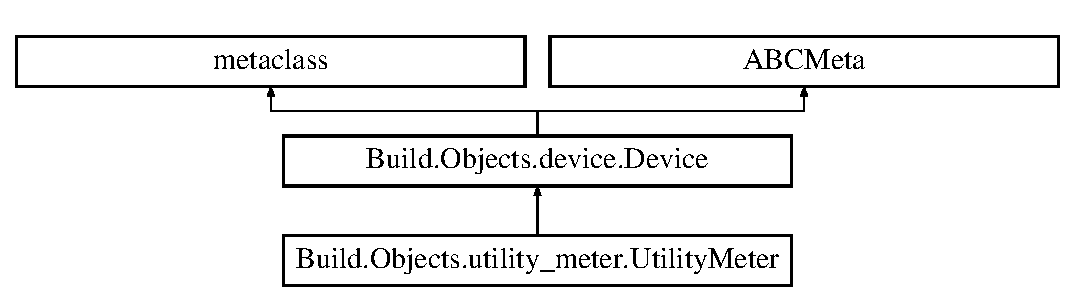
\includegraphics[height=3.000000cm]{class_build_1_1_objects_1_1utility__meter_1_1_utility_meter}
\end{center}
\end{figure}
\subsection*{Public Member Functions}
\begin{DoxyCompactItemize}
\item 
\mbox{\Hypertarget{class_build_1_1_objects_1_1utility__meter_1_1_utility_meter_a641edf1c1c911d9e2cffe710d139782c}\label{class_build_1_1_objects_1_1utility__meter_1_1_utility_meter_a641edf1c1c911d9e2cffe710d139782c}} 
def {\bfseries \+\_\+\+\_\+init\+\_\+\+\_\+} (self, device\+\_\+id, supervisor, msg\+\_\+latency=0, schedule=None, runtime=S\+E\+C\+O\+N\+D\+S\+\_\+\+I\+N\+\_\+\+D\+AY, multiday=0, sell\+\_\+price\+\_\+schedule=None, sell\+\_\+price\+\_\+multiday=0, buy\+\_\+price\+\_\+schedule=None, buy\+\_\+price\+\_\+multiday=0, connected\+\_\+devices=None)
\item 
def \hyperlink{class_build_1_1_objects_1_1utility__meter_1_1_utility_meter_a426b005fc2ad0ce41094d80e324a251f}{turn\+\_\+on} (self)
\begin{DoxyCompactList}\small\item\em Turn the utility meter on so that it can provide and receive power. \end{DoxyCompactList}\item 
def \hyperlink{class_build_1_1_objects_1_1utility__meter_1_1_utility_meter_a33fc2489dff8710a37e6067238f30305}{turn\+\_\+off} (self)
\begin{DoxyCompactList}\small\item\em Turn the utility meter off so that it can no longer provide and receive power. \end{DoxyCompactList}\item 
def \hyperlink{class_build_1_1_objects_1_1utility__meter_1_1_utility_meter_a3fddd94d0a6ca8646c64a5684e447e0d}{set\+\_\+sell\+\_\+price} (self, sell\+\_\+price)
\begin{DoxyCompactList}\small\item\em Change the sell price for this utility meter. \end{DoxyCompactList}\item 
def \hyperlink{class_build_1_1_objects_1_1utility__meter_1_1_utility_meter_a251bb69419a9885a8e867d8b5932c044}{set\+\_\+buy\+\_\+price} (self, buy\+\_\+price)
\begin{DoxyCompactList}\small\item\em Sets the buy price for this utility meter. \end{DoxyCompactList}\item 
def \hyperlink{class_build_1_1_objects_1_1utility__meter_1_1_utility_meter_a197ab2ab7f5abe14619a2ae15898b074}{setup\+\_\+price\+\_\+schedules} (self, sell\+\_\+price\+\_\+schedule, buy\+\_\+price\+\_\+schedule, sell\+\_\+price\+\_\+multiday=0, buy\+\_\+price\+\_\+multiday=0, runtime=S\+E\+C\+O\+N\+D\+S\+\_\+\+I\+N\+\_\+\+D\+AY)
\begin{DoxyCompactList}\small\item\em Adds a price schedule for this utility  sell\+\_\+price\+\_\+schedule the list of hour, sell\+\_\+price tuples in. \end{DoxyCompactList}\item 
def \hyperlink{class_build_1_1_objects_1_1utility__meter_1_1_utility_meter_a498d637ea147a783280bc68594ef0069}{process\+\_\+power\+\_\+message} (self, sender\+\_\+id, new\+\_\+power)
\begin{DoxyCompactList}\small\item\em Process a power message from a grid controller. \end{DoxyCompactList}\item 
def \hyperlink{class_build_1_1_objects_1_1utility__meter_1_1_utility_meter_a44b7bc4b09471d2529d4fef6c07abc42}{process\+\_\+price\+\_\+message} (self, sender\+\_\+id, new\+\_\+price, extra\+\_\+info)
\begin{DoxyCompactList}\small\item\em Method to be called when device receives a price message. \end{DoxyCompactList}\item 
def \hyperlink{class_build_1_1_objects_1_1utility__meter_1_1_utility_meter_ae450ec6bdd72caebb6163ae05490a1f8}{process\+\_\+request\+\_\+message} (self, sender\+\_\+id, request\+\_\+amt)
\begin{DoxyCompactList}\small\item\em Method to be called when device receives a request message, indicating a device is requesting to either provide or receive the requested quantity of power. \end{DoxyCompactList}\item 
def \hyperlink{class_build_1_1_objects_1_1utility__meter_1_1_utility_meter_a8b7c3c518352e0a41555a1a9e70b460c}{process\+\_\+allocate\+\_\+message} (self, sender\+\_\+id, allocate\+\_\+amt)
\begin{DoxyCompactList}\small\item\em Utility Meter does not process allocate messages. \end{DoxyCompactList}\item 
def \hyperlink{class_build_1_1_objects_1_1utility__meter_1_1_utility_meter_adc1f007ca7702f7db08c7238e2cead00}{send\+\_\+power\+\_\+message} (self, target\+\_\+id, power\+\_\+amt)
\begin{DoxyCompactList}\small\item\em This utility meter sends a power message to another device indicating that a certain quantity of power is now flowing across the link. \end{DoxyCompactList}\item 
def \hyperlink{class_build_1_1_objects_1_1utility__meter_1_1_utility_meter_adc776ffbce82fa1dc11ed6ec012d768d}{send\+\_\+price\+\_\+message} (self, target\+\_\+id, sell\+\_\+price, buy\+\_\+price)
\begin{DoxyCompactList}\small\item\em This utility meter informs another device of both its current buy price and its current sell price. \end{DoxyCompactList}\item 
def \hyperlink{class_build_1_1_objects_1_1utility__meter_1_1_utility_meter_a6d5719f08ebc1a80f95a33f77de27a7c}{broadcast\+\_\+price\+\_\+levels} (self, sell\+\_\+price, buy\+\_\+price)
\begin{DoxyCompactList}\small\item\em Informs all connected devices of the utility meter\textquotesingle{}s buy price. \end{DoxyCompactList}\item 
\mbox{\Hypertarget{class_build_1_1_objects_1_1utility__meter_1_1_utility_meter_af364127959babff26c2385e52c915f46}\label{class_build_1_1_objects_1_1utility__meter_1_1_utility_meter_af364127959babff26c2385e52c915f46}} 
def \hyperlink{class_build_1_1_objects_1_1utility__meter_1_1_utility_meter_af364127959babff26c2385e52c915f46}{device\+\_\+specific\+\_\+calcs} (self)
\begin{DoxyCompactList}\small\item\em Utility meter currently does not have any specific device calculations to add to the log file. \end{DoxyCompactList}\end{DoxyCompactItemize}


\subsection{Member Function Documentation}
\mbox{\Hypertarget{class_build_1_1_objects_1_1utility__meter_1_1_utility_meter_a6d5719f08ebc1a80f95a33f77de27a7c}\label{class_build_1_1_objects_1_1utility__meter_1_1_utility_meter_a6d5719f08ebc1a80f95a33f77de27a7c}} 
\index{Build\+::\+Objects\+::utility\+\_\+meter\+::\+Utility\+Meter@{Build\+::\+Objects\+::utility\+\_\+meter\+::\+Utility\+Meter}!broadcast\+\_\+price\+\_\+levels@{broadcast\+\_\+price\+\_\+levels}}
\index{broadcast\+\_\+price\+\_\+levels@{broadcast\+\_\+price\+\_\+levels}!Build\+::\+Objects\+::utility\+\_\+meter\+::\+Utility\+Meter@{Build\+::\+Objects\+::utility\+\_\+meter\+::\+Utility\+Meter}}
\subsubsection{\texorpdfstring{broadcast\+\_\+price\+\_\+levels()}{broadcast\_price\_levels()}}
{\footnotesize\ttfamily def Build.\+Objects.\+utility\+\_\+meter.\+Utility\+Meter.\+broadcast\+\_\+price\+\_\+levels (\begin{DoxyParamCaption}\item[{}]{self,  }\item[{}]{sell\+\_\+price,  }\item[{}]{buy\+\_\+price }\end{DoxyParamCaption})}



Informs all connected devices of the utility meter\textquotesingle{}s buy price. 


\begin{DoxyParams}{Parameters}
{\em price} & the price to broadcast to all connected devices \\
\hline
\end{DoxyParams}
\mbox{\Hypertarget{class_build_1_1_objects_1_1utility__meter_1_1_utility_meter_a8b7c3c518352e0a41555a1a9e70b460c}\label{class_build_1_1_objects_1_1utility__meter_1_1_utility_meter_a8b7c3c518352e0a41555a1a9e70b460c}} 
\index{Build\+::\+Objects\+::utility\+\_\+meter\+::\+Utility\+Meter@{Build\+::\+Objects\+::utility\+\_\+meter\+::\+Utility\+Meter}!process\+\_\+allocate\+\_\+message@{process\+\_\+allocate\+\_\+message}}
\index{process\+\_\+allocate\+\_\+message@{process\+\_\+allocate\+\_\+message}!Build\+::\+Objects\+::utility\+\_\+meter\+::\+Utility\+Meter@{Build\+::\+Objects\+::utility\+\_\+meter\+::\+Utility\+Meter}}
\subsubsection{\texorpdfstring{process\+\_\+allocate\+\_\+message()}{process\_allocate\_message()}}
{\footnotesize\ttfamily def Build.\+Objects.\+utility\+\_\+meter.\+Utility\+Meter.\+process\+\_\+allocate\+\_\+message (\begin{DoxyParamCaption}\item[{}]{self,  }\item[{}]{sender\+\_\+id,  }\item[{}]{allocate\+\_\+amt }\end{DoxyParamCaption})}



Utility Meter does not process allocate messages. 


\begin{DoxyParams}{Parameters}
{\em sender\+\_\+id} & the sender of the allocate message \\
\hline
{\em allocate\+\_\+amt} & the quantity that this device has been allocated to consume \\
\hline
\end{DoxyParams}
\mbox{\Hypertarget{class_build_1_1_objects_1_1utility__meter_1_1_utility_meter_a498d637ea147a783280bc68594ef0069}\label{class_build_1_1_objects_1_1utility__meter_1_1_utility_meter_a498d637ea147a783280bc68594ef0069}} 
\index{Build\+::\+Objects\+::utility\+\_\+meter\+::\+Utility\+Meter@{Build\+::\+Objects\+::utility\+\_\+meter\+::\+Utility\+Meter}!process\+\_\+power\+\_\+message@{process\+\_\+power\+\_\+message}}
\index{process\+\_\+power\+\_\+message@{process\+\_\+power\+\_\+message}!Build\+::\+Objects\+::utility\+\_\+meter\+::\+Utility\+Meter@{Build\+::\+Objects\+::utility\+\_\+meter\+::\+Utility\+Meter}}
\subsubsection{\texorpdfstring{process\+\_\+power\+\_\+message()}{process\_power\_message()}}
{\footnotesize\ttfamily def Build.\+Objects.\+utility\+\_\+meter.\+Utility\+Meter.\+process\+\_\+power\+\_\+message (\begin{DoxyParamCaption}\item[{}]{self,  }\item[{}]{sender\+\_\+id,  }\item[{}]{new\+\_\+power }\end{DoxyParamCaption})}



Process a power message from a grid controller. 

If this utility meter is operational, always provide what is demanded, assuming amount less than maximum output capacity. 
\begin{DoxyParams}{Parameters}
{\em sender\+\_\+id} & the \\
\hline
{\em new\+\_\+power} & the new power from the sender\textquotesingle{}s perspective \\
\hline
\end{DoxyParams}
\mbox{\Hypertarget{class_build_1_1_objects_1_1utility__meter_1_1_utility_meter_a44b7bc4b09471d2529d4fef6c07abc42}\label{class_build_1_1_objects_1_1utility__meter_1_1_utility_meter_a44b7bc4b09471d2529d4fef6c07abc42}} 
\index{Build\+::\+Objects\+::utility\+\_\+meter\+::\+Utility\+Meter@{Build\+::\+Objects\+::utility\+\_\+meter\+::\+Utility\+Meter}!process\+\_\+price\+\_\+message@{process\+\_\+price\+\_\+message}}
\index{process\+\_\+price\+\_\+message@{process\+\_\+price\+\_\+message}!Build\+::\+Objects\+::utility\+\_\+meter\+::\+Utility\+Meter@{Build\+::\+Objects\+::utility\+\_\+meter\+::\+Utility\+Meter}}
\subsubsection{\texorpdfstring{process\+\_\+price\+\_\+message()}{process\_price\_message()}}
{\footnotesize\ttfamily def Build.\+Objects.\+utility\+\_\+meter.\+Utility\+Meter.\+process\+\_\+price\+\_\+message (\begin{DoxyParamCaption}\item[{}]{self,  }\item[{}]{sender\+\_\+id,  }\item[{}]{new\+\_\+price,  }\item[{}]{extra\+\_\+info }\end{DoxyParamCaption})}



Method to be called when device receives a price message. 


\begin{DoxyParams}{Parameters}
{\em new\+\_\+price} & the new price value \\
\hline
\end{DoxyParams}
\mbox{\Hypertarget{class_build_1_1_objects_1_1utility__meter_1_1_utility_meter_ae450ec6bdd72caebb6163ae05490a1f8}\label{class_build_1_1_objects_1_1utility__meter_1_1_utility_meter_ae450ec6bdd72caebb6163ae05490a1f8}} 
\index{Build\+::\+Objects\+::utility\+\_\+meter\+::\+Utility\+Meter@{Build\+::\+Objects\+::utility\+\_\+meter\+::\+Utility\+Meter}!process\+\_\+request\+\_\+message@{process\+\_\+request\+\_\+message}}
\index{process\+\_\+request\+\_\+message@{process\+\_\+request\+\_\+message}!Build\+::\+Objects\+::utility\+\_\+meter\+::\+Utility\+Meter@{Build\+::\+Objects\+::utility\+\_\+meter\+::\+Utility\+Meter}}
\subsubsection{\texorpdfstring{process\+\_\+request\+\_\+message()}{process\_request\_message()}}
{\footnotesize\ttfamily def Build.\+Objects.\+utility\+\_\+meter.\+Utility\+Meter.\+process\+\_\+request\+\_\+message (\begin{DoxyParamCaption}\item[{}]{self,  }\item[{}]{sender\+\_\+id,  }\item[{}]{request\+\_\+amt }\end{DoxyParamCaption})}



Method to be called when device receives a request message, indicating a device is requesting to either provide or receive the requested quantity of power. 


\begin{DoxyParams}{Parameters}
{\em request\+\_\+amt} & the amount the sender is requesting to provide (positive) or to receive (negative). \\
\hline
\end{DoxyParams}
\mbox{\Hypertarget{class_build_1_1_objects_1_1utility__meter_1_1_utility_meter_adc1f007ca7702f7db08c7238e2cead00}\label{class_build_1_1_objects_1_1utility__meter_1_1_utility_meter_adc1f007ca7702f7db08c7238e2cead00}} 
\index{Build\+::\+Objects\+::utility\+\_\+meter\+::\+Utility\+Meter@{Build\+::\+Objects\+::utility\+\_\+meter\+::\+Utility\+Meter}!send\+\_\+power\+\_\+message@{send\+\_\+power\+\_\+message}}
\index{send\+\_\+power\+\_\+message@{send\+\_\+power\+\_\+message}!Build\+::\+Objects\+::utility\+\_\+meter\+::\+Utility\+Meter@{Build\+::\+Objects\+::utility\+\_\+meter\+::\+Utility\+Meter}}
\subsubsection{\texorpdfstring{send\+\_\+power\+\_\+message()}{send\_power\_message()}}
{\footnotesize\ttfamily def Build.\+Objects.\+utility\+\_\+meter.\+Utility\+Meter.\+send\+\_\+power\+\_\+message (\begin{DoxyParamCaption}\item[{}]{self,  }\item[{}]{target\+\_\+id,  }\item[{}]{power\+\_\+amt }\end{DoxyParamCaption})}



This utility meter sends a power message to another device indicating that a certain quantity of power is now flowing across the link. 

This message should only be in response to receiving a power msg to inform that it must provide a different amount than what was asked. \mbox{\Hypertarget{class_build_1_1_objects_1_1utility__meter_1_1_utility_meter_adc776ffbce82fa1dc11ed6ec012d768d}\label{class_build_1_1_objects_1_1utility__meter_1_1_utility_meter_adc776ffbce82fa1dc11ed6ec012d768d}} 
\index{Build\+::\+Objects\+::utility\+\_\+meter\+::\+Utility\+Meter@{Build\+::\+Objects\+::utility\+\_\+meter\+::\+Utility\+Meter}!send\+\_\+price\+\_\+message@{send\+\_\+price\+\_\+message}}
\index{send\+\_\+price\+\_\+message@{send\+\_\+price\+\_\+message}!Build\+::\+Objects\+::utility\+\_\+meter\+::\+Utility\+Meter@{Build\+::\+Objects\+::utility\+\_\+meter\+::\+Utility\+Meter}}
\subsubsection{\texorpdfstring{send\+\_\+price\+\_\+message()}{send\_price\_message()}}
{\footnotesize\ttfamily def Build.\+Objects.\+utility\+\_\+meter.\+Utility\+Meter.\+send\+\_\+price\+\_\+message (\begin{DoxyParamCaption}\item[{}]{self,  }\item[{}]{target\+\_\+id,  }\item[{}]{sell\+\_\+price,  }\item[{}]{buy\+\_\+price }\end{DoxyParamCaption})}



This utility meter informs another device of both its current buy price and its current sell price. 

The buy price information is contained in the message\textquotesingle{}s extra\+\_\+info field. \mbox{\Hypertarget{class_build_1_1_objects_1_1utility__meter_1_1_utility_meter_a251bb69419a9885a8e867d8b5932c044}\label{class_build_1_1_objects_1_1utility__meter_1_1_utility_meter_a251bb69419a9885a8e867d8b5932c044}} 
\index{Build\+::\+Objects\+::utility\+\_\+meter\+::\+Utility\+Meter@{Build\+::\+Objects\+::utility\+\_\+meter\+::\+Utility\+Meter}!set\+\_\+buy\+\_\+price@{set\+\_\+buy\+\_\+price}}
\index{set\+\_\+buy\+\_\+price@{set\+\_\+buy\+\_\+price}!Build\+::\+Objects\+::utility\+\_\+meter\+::\+Utility\+Meter@{Build\+::\+Objects\+::utility\+\_\+meter\+::\+Utility\+Meter}}
\subsubsection{\texorpdfstring{set\+\_\+buy\+\_\+price()}{set\_buy\_price()}}
{\footnotesize\ttfamily def Build.\+Objects.\+utility\+\_\+meter.\+Utility\+Meter.\+set\+\_\+buy\+\_\+price (\begin{DoxyParamCaption}\item[{}]{self,  }\item[{}]{buy\+\_\+price }\end{DoxyParamCaption})}



Sets the buy price for this utility meter. 


\begin{DoxyParams}{Parameters}
{\em buy\+\_\+price} & the buy price to set the value to \\
\hline
\end{DoxyParams}
\mbox{\Hypertarget{class_build_1_1_objects_1_1utility__meter_1_1_utility_meter_a3fddd94d0a6ca8646c64a5684e447e0d}\label{class_build_1_1_objects_1_1utility__meter_1_1_utility_meter_a3fddd94d0a6ca8646c64a5684e447e0d}} 
\index{Build\+::\+Objects\+::utility\+\_\+meter\+::\+Utility\+Meter@{Build\+::\+Objects\+::utility\+\_\+meter\+::\+Utility\+Meter}!set\+\_\+sell\+\_\+price@{set\+\_\+sell\+\_\+price}}
\index{set\+\_\+sell\+\_\+price@{set\+\_\+sell\+\_\+price}!Build\+::\+Objects\+::utility\+\_\+meter\+::\+Utility\+Meter@{Build\+::\+Objects\+::utility\+\_\+meter\+::\+Utility\+Meter}}
\subsubsection{\texorpdfstring{set\+\_\+sell\+\_\+price()}{set\_sell\_price()}}
{\footnotesize\ttfamily def Build.\+Objects.\+utility\+\_\+meter.\+Utility\+Meter.\+set\+\_\+sell\+\_\+price (\begin{DoxyParamCaption}\item[{}]{self,  }\item[{}]{sell\+\_\+price }\end{DoxyParamCaption})}



Change the sell price for this utility meter. 


\begin{DoxyParams}{Parameters}
{\em sell\+\_\+price} & the sell price to set the value to \\
\hline
\end{DoxyParams}
\mbox{\Hypertarget{class_build_1_1_objects_1_1utility__meter_1_1_utility_meter_a197ab2ab7f5abe14619a2ae15898b074}\label{class_build_1_1_objects_1_1utility__meter_1_1_utility_meter_a197ab2ab7f5abe14619a2ae15898b074}} 
\index{Build\+::\+Objects\+::utility\+\_\+meter\+::\+Utility\+Meter@{Build\+::\+Objects\+::utility\+\_\+meter\+::\+Utility\+Meter}!setup\+\_\+price\+\_\+schedules@{setup\+\_\+price\+\_\+schedules}}
\index{setup\+\_\+price\+\_\+schedules@{setup\+\_\+price\+\_\+schedules}!Build\+::\+Objects\+::utility\+\_\+meter\+::\+Utility\+Meter@{Build\+::\+Objects\+::utility\+\_\+meter\+::\+Utility\+Meter}}
\subsubsection{\texorpdfstring{setup\+\_\+price\+\_\+schedules()}{setup\_price\_schedules()}}
{\footnotesize\ttfamily def Build.\+Objects.\+utility\+\_\+meter.\+Utility\+Meter.\+setup\+\_\+price\+\_\+schedules (\begin{DoxyParamCaption}\item[{}]{self,  }\item[{}]{sell\+\_\+price\+\_\+schedule,  }\item[{}]{buy\+\_\+price\+\_\+schedule,  }\item[{}]{sell\+\_\+price\+\_\+multiday = {\ttfamily 0},  }\item[{}]{buy\+\_\+price\+\_\+multiday = {\ttfamily 0},  }\item[{}]{runtime = {\ttfamily SECONDS\+\_\+IN\+\_\+DAY} }\end{DoxyParamCaption})}



Adds a price schedule for this utility  sell\+\_\+price\+\_\+schedule the list of hour, sell\+\_\+price tuples in. 


\begin{DoxyParams}{Parameters}
{\em multiday} & how many days of the scheduling to set as a repeating \\
\hline
\end{DoxyParams}
\mbox{\Hypertarget{class_build_1_1_objects_1_1utility__meter_1_1_utility_meter_a33fc2489dff8710a37e6067238f30305}\label{class_build_1_1_objects_1_1utility__meter_1_1_utility_meter_a33fc2489dff8710a37e6067238f30305}} 
\index{Build\+::\+Objects\+::utility\+\_\+meter\+::\+Utility\+Meter@{Build\+::\+Objects\+::utility\+\_\+meter\+::\+Utility\+Meter}!turn\+\_\+off@{turn\+\_\+off}}
\index{turn\+\_\+off@{turn\+\_\+off}!Build\+::\+Objects\+::utility\+\_\+meter\+::\+Utility\+Meter@{Build\+::\+Objects\+::utility\+\_\+meter\+::\+Utility\+Meter}}
\subsubsection{\texorpdfstring{turn\+\_\+off()}{turn\_off()}}
{\footnotesize\ttfamily def Build.\+Objects.\+utility\+\_\+meter.\+Utility\+Meter.\+turn\+\_\+off (\begin{DoxyParamCaption}\item[{}]{self }\end{DoxyParamCaption})}



Turn the utility meter off so that it can no longer provide and receive power. 

\mbox{\Hypertarget{class_build_1_1_objects_1_1utility__meter_1_1_utility_meter_a426b005fc2ad0ce41094d80e324a251f}\label{class_build_1_1_objects_1_1utility__meter_1_1_utility_meter_a426b005fc2ad0ce41094d80e324a251f}} 
\index{Build\+::\+Objects\+::utility\+\_\+meter\+::\+Utility\+Meter@{Build\+::\+Objects\+::utility\+\_\+meter\+::\+Utility\+Meter}!turn\+\_\+on@{turn\+\_\+on}}
\index{turn\+\_\+on@{turn\+\_\+on}!Build\+::\+Objects\+::utility\+\_\+meter\+::\+Utility\+Meter@{Build\+::\+Objects\+::utility\+\_\+meter\+::\+Utility\+Meter}}
\subsubsection{\texorpdfstring{turn\+\_\+on()}{turn\_on()}}
{\footnotesize\ttfamily def Build.\+Objects.\+utility\+\_\+meter.\+Utility\+Meter.\+turn\+\_\+on (\begin{DoxyParamCaption}\item[{}]{self }\end{DoxyParamCaption})}



Turn the utility meter on so that it can provide and receive power. 



The documentation for this class was generated from the following file\+:\begin{DoxyCompactItemize}
\item 
Build/\+Objects/utility\+\_\+meter.\+py\end{DoxyCompactItemize}

\hypertarget{class_build_1_1_objects_1_1wire_1_1_wire}{}\section{Build.\+Objects.\+wire.\+Wire Class Reference}
\label{class_build_1_1_objects_1_1wire_1_1_wire}\index{Build.\+Objects.\+wire.\+Wire@{Build.\+Objects.\+wire.\+Wire}}
\subsection*{Public Member Functions}
\begin{DoxyCompactItemize}
\item 
\mbox{\Hypertarget{class_build_1_1_objects_1_1wire_1_1_wire_a08fcb1c42a58e7f7102417032aec3fd4}\label{class_build_1_1_objects_1_1wire_1_1_wire_a08fcb1c42a58e7f7102417032aec3fd4}} 
def {\bfseries \+\_\+\+\_\+init\+\_\+\+\_\+} (self, length, thickness, resistance)
\end{DoxyCompactItemize}


The documentation for this class was generated from the following file\+:\begin{DoxyCompactItemize}
\item 
Build/\+Objects/wire.\+py\end{DoxyCompactItemize}

%--- End generated contents ---

% Index
\backmatter
\newpage
\phantomsection
\clearemptydoublepage
\addcontentsline{toc}{chapter}{Index}
\printindex

\end{document}
